\documentclass[12pt,  a4paper,oneside]{book} %Fjern twoside dersom\usepackage[norsk] skriveren kun skriver ut på én side
% Pakker.
\usepackage[paper=A4,pagesize]{typearea}
\usepackage{titlesec}
\usepackage{times}
\usepackage[utf8]{inputenc}
\usepackage[english]{babel}
\usepackage{textcomp}
\usepackage{siunitx}
\usepackage{multirow}
\usepackage{multicol}
\usepackage{wrapfig}
\usepackage{amsmath}
\usepackage{pdfpages}
\usepackage{csvsimple}
\usepackage{array}
\usepackage{colortbl}
\usepackage{afterpage}%bruker denne til å inkludere a3
\usepackage{pdflscape}%bruker denne til å rotere pdf
\usepackage{lscape}
\usepackage{parskip}
\usepackage[flushleft]{threeparttable} % for fotnoter til tabeller
\usepackage{rotating}
\usepackage{adjustbox}
\usepackage{setspace}

\usepackage{multicol}
% For hypertekst i pdf.
\usepackage[hidelinks]{hyperref} %Denne må før glossaries
%\providecommand\phantomsection{} % Denne gjor at det vil kompilere både med og uten hyperref som funker

% Innfører \cref{} for å gjøre referering til labler lettere.
\usepackage[english]{cleveref}
% Her kan man justere formateringen av kryssreferanser til cref:
    % Kappittel:
    \Crefformat{chapter}{Chapter~#2#1#3}
    \crefformat{chapter}{Chapter~#2#1#3}
    % Sections(og sub/subsub-sections):
    \Crefformat{section}{Section~#2#1#3}
    \crefformat{section}{Section~#2#1#3}
    % Figurer
    \Crefformat{figure}{Figure~#2#1#3}
    \crefformat{figure}{Figure~#2#1#3}
    % tabeller
    \Crefformat{table}{Table~#2#1#3}
    \crefformat{table}{Table~#2#1#3}
    % Appendixer
    \Crefformat{appendix}{Appendix~#2#1#3}
    \crefformat{appendix}{Appendix~#2#1#3}

\usepackage[acronym,xindy]{glossaries}
\usepackage{glossary-mcols}% glossaries med to kolonner
\renewcommand{\glossaryentrynumbers}[1]{}% empty sidetall best uten
%\makeglossaries

% Gjør lister bedre.
%\setlength{\parskip}{1.5em} %avstand mellom avsnitt
%\renewcommand{\baselinestretch}{1.5} %linjeavstand
% Laster fonten Latin Modern.

\usepackage{verbatim} %kommentere ut blokker med \begin{comment} .... \end{comment}
\usepackage{nomencl}
% Forsøk på å lage symbolliste
\usepackage[bottom]{footmisc} 

\usepackage{lmodern}

\usepackage{amsmath,amssymb}
% Innfører \ce{} for å gjøre kjemiske ligninger fine.
\usepackage[version=3]{mhchem}
% Gjør tabeller bedre.
\usepackage{tabularx}
\usepackage{booktabs,caption}
\usepackage{array}
\usepackage{textgreek}


% Gjør figurer og bilder bedre.
\usepackage{float}
\usepackage{graphicx}
% Gjør så man kan innføre koder som Matlab script (se prosessprodjekt for eksempel).
\usepackage{listings}
% For å tegne grafikk direkte i tex (kan feks innføre DIA diagrammer med tikz).
%\usepackage{tikz}
% For å få inn tex-filer fra matlab2tikz.
%\usetikzlibrary{external}
%\tikzexternalize[prefix=Bilder/Diagrammer/TikzFigs/]%lagrer pdfer her men vises ikke (bare lastes etter generering en gang) DEtte utgår
\usepackage{chemfig}
\usepackage{pgfplots}
\usepackage{pgffor}

\usepackage[utf8]{inputenc}
\usepackage{dirtytalk} 
\pgfplotsset{compat=newest}
\pgfplotsset{plot coordinates/math parser=false}
\newlength\figureheight
\newlength\figurewidth

% Gir funksjoner for en bedre topp- og bunntekst (Header og footer).
\usepackage{fancyhdr}
% Ordner funksjoner for format.
\usepackage[left=2cm, right=2cm, top=2cm]{geometry}%kan justere marg avstand og "textwidt"

% Gir labler fet tekst feks. \textbf{FIGUR 1.2:} oppsett av utstyr.
\usepackage[labelfont=bf]{caption}
\usepackage{subcaption}

\usepackage{float}
\floatstyle{plaintop}
\restylefloat{table}

% Ordner nummerering av floats innenfor sine respektable avsnitt.
\numberwithin{figure}{chapter}
\numberwithin{equation}{chapter}
\numberwithin{table}{chapter}


\usepackage{xcolor}
 %%%%%%%%
\usepackage{listings}  %%%!!!!!

\usepackage{color} %red, green, blue, yellow, cyan, magenta, black, white
\definecolor{mygreen}{RGB}{28,172,0} % color values Red, Green, Blue
\definecolor{mylilas}{RGB}{170,55,241}
%%%%%%%%


\usepackage[authoryear,round]{natbib}
\bibliographystyle{agsm} %Harvard ish stil

%\usepackage[authoryear,round]{natbib}
\usepackage{enumitem}
%\hypersetup{pdfauthor={Egil}} % Denne skulle fikse noe...
\usepackage{newfloat} % Vil du ha vanlig telling velg "within=none". "within=section" gir nummerering "section.<skjemanummer>". Skriver du i memoir/book/e.l. med chapter som hovedkapittel, kan det være naturlig å velge "within=chapter" i stedet.

\DeclareFloatingEnvironment[  fileext={skjema},  placement={!htbp},  name={Skjema},  listname={Skjemaliste}]{skjema}
% jeg er fæn av å holde figurer på Topp, Bunn eller egen Page, men hvis du vil bruke !h også kan du endre til "placement={!htbp}"
\numberwithin{skjema}{section}

\usepackage{changepage}


\begin{document}
%TC:ignore
% Forside
\pagenumbering{gobble} %skrur av sidetall
%\include{Chapters/0-Div/Forside}


%\pagenumbering{arabic} %sidetall etter innholdsfortegnelse
\pagestyle{plain}
\pagenumbering{roman}
\setcounter{page}{5}
%\include{Chapters/0-Div/preface}
%\includepdf{Chapters/0-Div/PREFACE_signert.PDF}
\newpage
\addcontentsline{toc}{chapter}{Acknowledgements}
\section*{Acknowledgements}
I would like to express my deepest gratitude to the Norwegian Geotechnical Institute (NGI) who let me conduct all of my tests in their environmental chemistry laboratory.

Erlend Sørmo
Gerard Cornelissen
Egil, Marit, Christian introducing me to  \LaTeX and helping with formatting.

Aurora Hofman and Raol Wolf for help with coding in R

Gabriela Castro Varela for sample processing at NTNU with SPE and LC-MS/MS

Michel Hubert

Hans Peter Arp

\include{Chapters/0-Div/Summary}
\newpage
\addcontentsline{toc}{chapter}{Sammendrag}
\section*{Sammendrag}





\listoffigures
\addcontentsline{toc}{chapter}{List of figures}
%\clearpage

\listoftables
\addcontentsline{toc}{chapter}{List of tables}
%\clearpage

\newacronym{DOC}{DOC}{dissolved organic carbon}
\newacronym{TOC}{TOC}{total organic carbon}
\newacronym{CWC}{CWC}{clean wood chips}
\newacronym{ULS}{ULS}{Ullensaker sludge}
\newacronym{DSL}{DSL}{digested sludge Lindum}
\newacronym{EDL}{EDL}{electrical double layer}
\newacronym{PFPeA}{PFPeA}{perfluoropentanoic acid}
\newacronym{PFHxA}{PFHxA}{perfluorohexanoic acid}
\newacronym{PFHpA}{PFHpA}{perfluoroheptanoic acid}
\newacronym{PFOA}{PFOA}{perfluorooctanoic acid}
\newacronym{PFNA}{PFNA}{perfluorononaoic acid}
\newacronym{PFDA}{PFDA}{perfluorodecanoic acid}
\newacronym{PFAS}{PFAS}{perfluorinated alkyl substances}
\newacronym{TC}{TC}{target compound}
\newacronym{TA}{TA}{target analyte}
\newacronym{BC}{BC}{biochar}
\newacronym{AC}{AC}{activated carbon}
\newacronym{ABC}{ABC}{activated biochar}
\newacronym{SC}{SC}{spike concentration (ref. SP)}
\newacronym{SP}{SP}{spike point (ref. SC)}
\newacronym{AD}{AD}{anaerobic digestion}
\newacronym{PT}{PT}{pyrolysis temperature}
\newacronym{RT}{RT}{residence time}
\newacronym{BJH}{BJH}{}
\newacronym{DFT}{DFT}{density-functional theory}
\newacronym{BET}{BET}{}
\newacronym{EXAFS}{EXAFS}{Extended X-ray Absorption Fine Structure}
\newacronym{LC-MS/MS}{LC-MS/MS}{}
\newacronym{LOQ}{LOQ}{}
\newacronym{LOD}{LOD}{}
\newacronym{MIX}{MIX}{}
\newacronym{SPE}{SPE}{}
\newacronym{MeOH}{MeOH}{}
\newacronym{MQ}{MQ}{}
\newacronym{QA}{QA}{}
\newacronym{QC}{QC}{}
\newacronym{CEC}{CEC}{}
\newacronym{SA}{SA}{}
\newacronym{PV}{PV}{}
\newacronym{PSD}{PSD}{}
\newacronym{PZC}{PZC}{}
\newacronym{OM}{OM}{}
\newacronym{LCIA}{LCIA}{}
\newacronym{SDGs}{SDGs}{}
\newacronym{EXANES}{EXANES}{X-ray Absorption Near Edge Structure}
\newacronym{PP}{}{}
\newacronym{NGI}{NGI}{Norwegian Geotechnical Institute}
\newacronym{VOW}{VOW}{Valorization of Organic Waste}

\printglossary[type=\acronymtype, style=mcolindex, title=Acronyms] 

 	



\addcontentsline{toc}{chapter}{Acronyms}
%\clearpage

\clearpage
\makenomenclature

\nomenclature{$C_w$}{aqueous equilibrium concentration}
\nomenclature{$C_s$}{sorbed equilibrium concentration}
\nomenclature{$C_i$}{initial concentration}
\nomenclature{$K_{OC}$}{organic carbon-water partition coefficient}
\nomenclature{$K_{OW}$}{octanol-water partition coefficient}
\nomenclature{$K_F$}{Freundlich partition coefficient}
\nomenclature{$n_F$}{Freundlich coefficient of non-linearity}
\nomenclature{$pK_a$}{acid dissociation constant}
\nomenclature{$D_{eff}$}{effective cross-sectional diameter of a molecule}
\nomenclature{$D_{max}$}{maximum diameter of a molecule}
\nomenclature{$K_{AW}$}{air-water parition coefficient}
\nomenclature{$K_F$}{Freundlich distribution coefficient}
\nomenclature{$n_F$}{Freundlich coefficient of non-linearity ($<1$)}






\renewcommand{\nomname}{Symbols}


\newcommand{\nomunit}[1]{%
  \renewcommand{\nomentryend}{\hspace*{\fill}#1}%
}

\printnomenclature[6em]

\addcontentsline{toc}{chapter}{Symbols}
%\clearpage

%TC:endignore

\newpage

\tableofcontents
\cleardoublepage


\pagenumbering{arabic}


% Topptekst.
\pagestyle{fancy}
\lhead{\leftmark}
\chead{}
\rhead{Krahn}
\renewcommand{\headrulewidth}{0.4pt}
% Slik at tekst ikke ligger for nærme toppteksten.
\setlength{\headheight}{30pt}



%\maketitle

\part{Introduction}
%Introduction:
%\chapter{Introduction}
\chapter{Introduction}\label{chap:intro}

Transport of contaminants.

Sewage sludge contains environmental pollutants and there is much concern recently related to spread of environmental pollutants through sewage sludge. If the findings in this study can be used to may provide promising outlooks for limiting spread of pollutants to the environment and rather valorizing the waste to sequester carbon and remediate contaminated sites.

Per- and polyfluoroalkyl substances (PFAS) used in aqueous film forming foam (AFFF) contaminates soil, groundwater, surface water and drinking water. Firefighting training site at Gardermoen, Norway used these substances since 1989. Been banned with new guidelines and regulations but there is still much left in the unsaturated zone heavily contaminated with PFAS (what are the concentrations of the various PFASs?) NGI document? 

POPS, PAHs, PBT properties, Stockholm Convention (2001)

PFAS uses

Human exposure: coating on clothing, drinking water, kitchen equipment, food packaging, herbicides, accumulation in food products, 

Environmental Quality Standards (EQS) - Miljødirektoratet \citep{EC2020PFAS}. \citep{MD2016workshop} \citep{MD2020EQS}

What is new: sorption of PFAS to sludge biochars is not yet studied. sludge char is being sold as soil amendment but cannot sell for as much money as sludge char as sorbent! Sorbents are more expensive. The results from this study may provide important economic advantages for Scanship and Lindum that can sell sludge char as sorbents for organic pollutants. The aim of the laboratory investigations was to characterize the PFCA sorption ability of biochars produced from waste materials to determine if such biochars can introduced to the market as sorbents. 

Important for wastewater treatment because. The use of biochar as sorbent for organic and inorganic contaminants has received increased attention in recent years. Biochar for soil remediation is becoming a particularly attractive concept due to a combined effect of serving as a similar effective sorbent as activated carbon combined with the major potential for carbon sequestration and eliminates the need for energy-intensive sewage sludge treatment. Biochar has received increased scientific and public attention in recent years for its sorptive abilities of various contaminants (both heavy metals and organic compounds) which are similar to activated carbon combined with the major potential for carbon sequestration. Commercial production is growing internationally and is now widely used for soil remediation \citep{Ahmad2014}. Low cost

%%%%%%%%%%%%%%%%%%%%%%%%%%%%%%%%%%%%%%%%%%%%%%%%%%%%%%%%%%%%%
\section{Background}\label{sec:Background}
 

%%%%%%%%%%%%%%%%%%%%%%%%%%%%%%%%%%%%%%%%%%%%%%%%%%%%%%%%%%%%%
\section{Objectives}
The overall goal of the study is to test if sewage sludge biochar can be used as an effective sorbent for PFAS in contaminated water and soils. Specifically, the objectives of this thesis are:
\begin{enumerate}
    \item {Provide a detailed mechanistic understanding of the sorption mechanisms of perfluorinated carboxylic acids of increasing chain lengths to waste biochar}
    \item{Provide a detailed mechanistic understanding of the sorption mechanisms of perfluorinated carboxylic acids of increasing chain lengths to a sandy, low-TOC soil amended with waste biochar}
    \item{Evaluate how a cocktail of PFCAs sorb to waste biochar compared with single PFCA compounds}
    \item{Evaluate if the waste biochars used in this study can be used to reduce naturally PFAS-contaminated to environmental quality standards set by the Norwegian government.}
\end{enumerate}

\subsection{Hypothesis}
The main hypothesis of this thesis was:
\textit{Sewage sludge biochar can serve as an effective sorbent for PFAS in contaminated water and soils.}

Three sub-hypotheses were tested:
\begin{itemize}
    \item PFAS sorption to sewage sludge biochar increases with chain length.
    \item When competition between PFASs in a cocktail is present, competition for sorption sites on the biochar occurs.
    \item When soil is amended with sewage sludge biochar, the sorption coefficient, K$_d$, will decrease somewhat compared to K$_d$ for sludge char alone due to attenuation by organic matter in the system. 
\end{itemize}
%%%%%%%%%%%%%%%%%%%%%%%%%%%%%%%%%%%%%%%%%%%%%%%%%%%%%%%%%%%%%
\section{Scope} 
What research has already been done on this subject? How does the work of this thesis stand out?
%%%%%%%%%%%%%%%%%%%%%%%%%%%%%%%%%%%%%%%%%%%%%%%%%%%%%%%%%%%%%
\section{Approach}
A literature study is aimed at...
Laboratory investigations are to be conducted to find... 

%%%%%%%%%%%%%%%%%%%%%%%%%%%%%%%%%%%%%%%%%%%%%%%%%%%%%%%%%%%%%
%Provides a list of the chapters and a short, one line description
\section{Structure of the document}
In \cref{chap:LitStudy} literature study, theory

In \cref{chap:MatlsMethds} the materials and methods are described and outlined.

In \cref{chap:Results&Disc} the results from laboratory testing are reported and discussed.

In \cref{chap:Conclusion} a conclusion of the work done in both lab and field is made.

In \cref{chap:furtherwork} recommendations for further work are proposed.
\newpage


%Literature
\chapter{Literature Study}\label{chap:LitStudy}
This chapter is a discussion of relevant literature for the work of this thesis with emphasis on the ecotoxicological risks of PFAS pollution in the environment and the application of biochar as sorbent for PFAS-contaminated soil and water.

\section{PFAS}
Per- and polyfluorinated alkyl substances---PFAS---are synthetic, oil- and water-repellent compounds that serve numerous applications in industrial and consumer products \citep{Nicole2013}. These include paint, coatings, firefighting foam, electronics, cosmetics, cookware, and textiles. Despite many desirable properties, the widespread production and use have distributed PFAS with waterways that end up in soil, crops, wildlife, and higher trophic levels including humans \citep{bhhatarai2011}. The persistency, bioaccumulation and toxicity in soil and water poses a major environmental concern that has led to legislative action on the manufacture, sale, and use of several PFAS compounds \citep{EPA2014,ECHA2020,EC2020PFAS}. Today, PFAS is recognized as an emerging contaminant \citep{Ryu2021EC}. By 2014, EPA listed PFOA and PFOS (and their salts) as emergent contaminants and began a phase-out DuPont "PFOA and PFOS have been listed under the Stockholm Convention on Persistent Organic Pollutants (POPs) and as a consequence, are now restricted under the EU POPs Regulation" and several other PFASs are being assessed for restriction under REACH and the Stockholm Convention \citep{EC2020PFAS}. Ongoing restriction of C9-C14 PFCAs under REACH (phased out before 2023) \citep{ECHA2020}. This section looks at the physicochemical properties, ecotoxicological risks, and transport and fate of PFAS in the environment.

\begin{figure}
    \centering
    \begin{tabular}{c}
    \chemname{\chemfig[atom style={scale=0.8}]{O=[:90](-[:30,,,1]OH)-[:150](-[:67.5]F)(-[:112.5]F)-[:210](-[:247.5]F)(-[:292.5]F)-[:150](-[:67.5]F)(-[:112.5]F)-[:210](-[:247.5]F)(-[:292.5]F)-[:150](-[:67.5]F)(-[:112.5]F)-[:210](-[:247.5]F)(-[:292.5]F)-[:150](-[:90]F)(-[:150]F)-[:210]F}}{perfluorooctanoic acid (PFOA)} \\
\\
    \chemname{\chemfig[atom style={scale=0.8}]{F-[:292.5](-[:67.5]F)(-[:330]S(=[:60]O)(-[:330,,,1]OH)=[:240]O)-[:210](-[:292.5]F)(-[:247.5]F)-[:150](-[:112.5]F)(-[:67.5]F)-[:210](-[:292.5]F)(-[:247.5]F)-[:150](-[:112.5]F)(-[:67.5]F)-[:210](-[:292.5]F)(-[:247.5]F)-[:150](-[:112.5]F)(-[:67.5]F)-[:210](-[:270]F)(-[:150]F)-[:210]F}}{perfluorooctanesufonic acid (PFOS)} \\
\\
    \chemname{\chemfig[atom style={scale=0.8}]{O=[:60]S(=[:60]O)(-[:330,,,1]OH)-[:150](-[:67.5]H)(-[:112.5]H)-[:210](-[:247.5]H)(-[:292.5]H)-[:150](-[:67.5]F)(-[:112.5]F)-[:210](-[:247.5]F)(-[:292.5]F)-[:150](-[:67.5]F)(-[:112.5]F)-[:210](-[:247.5]F)(-[:292.5]F)-[:150](-[:67.5]F)(-[:112.5]F)-[:210](-[:270]F)(-[:210]F)-[:150]F}}{6:2 fluorotelomer sulfonic acid (6:2 FTSA)} \\
\\
   %\chemname{
            %\chemleft
              %  \chemfig{
                   % -C
                      %  ( -[2]F)
                       % ( -[6]F)
                   % -C
                       % ( -[2]F)
                       % ( -[6]F)
                   % -[0]
               % }
           % \chemright]$_n$
       % }{polytetrafluoroethylene (PTFE)} \\
    \end{tabular}
    \caption{The most commonly studied and used PFAS compounds, PFOA, PFOS monomers and the polymer polytetrafluoroethylene used in non-stick, oil- and water-repellent products like Teflon and Gore-Tex.}
    \label{fig:PFASstruct}
\end{figure}
        
\subsection{Physicochemical properties}
PFAS are organic compounds that consist of a polar head, most commonly a carboxyl or sulfate
functional group, and a non-polar perfluoroalkyl chain of varying lengths of which either all
hydrogens (per-), or some (poly-) of the hydrogens bonded to carbon have been replaced with
fluorine atoms \citep{wang2011physchem}. Despite C-F bonds being highly polar (\textDelta \textchi=1.5), the symmetric structure of -CF$_2$- homologues makes the tail hydrophobic. PFCs are divided into compound classes based on the functional group attached to the chain, where the most common groups are perfluorinated carboxylic acids (PFCAs) and perfluorinated sulfonic acids (PFSAs) \cref{fig:PFASstruct}. The amphiphilic nature gives PFASs a set of unique and desirable properties as surfactants \citep{du2014adsorption}. These properties have made them ideal as foaming agents and flame retardants in firefighting foam (aqueous film forming foam (AFFF)) and as coating for the famous waterproof Gore-Tex\textsuperscript{\textregistered} textiles and non-stick, frictionless Teflon\textsuperscript{\texttrademark} cookware, but have also . 

\subsubsection{Intramolecular bonding}
PFASs are referred to as "forever chemicals" because they have an extremely high chemical and physical stability \citep{beans2021}. Since fluorine is a strong electrophile, the C-F covalent bonds make one of the strongest known bonds in organic chemistry (BDE=485 kJ mol\textsuperscript{-1}) \citep{Lau2007}. Since C-F bonds are not naturally found in the environment, there are few enzymes/microbes that can break them \citep{shahsavari2021}. Therefore, PFASs remain persistent molecules that stay in the environment "forever". 

\subsubsection{Intermolecular bonding}
The ability of PFCs to undergo van der Waals interactions can be modeled to say something about adsorption to hydrophobic surfaces in soils and sediment \citep{Arp2006}. Generally, these forces have shown to be insignificant for sorption of PFAS to solid phases for short-chain molecules (\textless C6) but is significant for long-chained PFCs (\textgreater C6) \citep{du2014adsorption}. In contrast to the lipophilic chain, the hydrophilic head can hydrogen bond to other polar compounds such as water and interact electrostatically with positively charged species. As surfactants, PFAS are soluble in water, but at high enough concentrations, the molecules arrange in micelles above the critical micelle concentration and the physicochemical behavior changes dramatically \citep{bhhatarai2011,Goss2009comment}.  

the speciation of the polar functional group on PFASs is affected by its surroundings---pH in particular. Generally, PFASs have low acid dissociation constants (\(K_a\)), and hence, appear as negatively charged in the environment \citep{Reemtsma2016}. Due to the hydrophobic tail, water solubility of PFASs are highly influenced by chain length where short-chain, PFCAs are have the highest solubility \citep{bhhatarai2011}.

\(pK_a\) values for PFCA homologues longer than C3 or C4 acid greatly decrease with increasing chain length. There has been some controversy related to the acid dissociation constants of PFAS, but it is now established that  \(pK_a\) values are greatly discussed/controversy in the scientific community \citep{Goss2009comment},  and is important because protonation affects the volatility of e.g. PFOA, which again affects mobility and spread of toxic contaminants \citep{Goss2009comment,wang2011physchem}. This issue is still not resolved, so p$K_a$ values range from 0-4 according to different researchers. 

\subsection{PFAS in water and soil}
In contrast to water solubility, sorption to soil and sediment plays an important role for retention and accumulation of PFAS in the environment \citep{li2018,LehmannAndJoseph2015,Cornelissen2005}. 
\(K_{OW}\) = octanol water partition coefficient used to say something about partitioning between a water phase and a hydrophobic phase (represented by octanol) \citep{Reemtsma2016}. For example, PFOA has a water solubility of 3.4 g L\textsuperscript{-1} \citep{PFOA} whereas its structural analog without the carboxylic end group is practically insoluble \citep{PFO}. The \(K_{OW}\) is therefore unique for PFAS compared to similar compounds   
Solubility and influences sorption mechanisms and mobility. PFCAs and other acidic PFASs appear in dissociated form due to low \(K_a\)'s at environmentally relevant pH's \citep{wang2011physchem}.
\cref{tab:COSMOtherm} gives an overview of different physicochemical properties of the PFCAs used for the research of this thesis modeled using COSMOterm by \cite{wang2011physchem}. 

Leaching to groundwater and surface water more than PAHs due to a lower partition coefficient ($K_{OC}$) than hydrocarbons, surfactants and the polar head makes them more mobile (more on this in \citep{du2014adsorption}). PFAS pollution of groundwater and soil is particularly prominent around several Norwegian airports where old firefighting training facilities uses fire-fighting foam containing PFAS \citep{MD2016workshop}. PFAS was the predominant compound used here and is now banned and replaced with other PFASs. 

Emerging contaminants definition \citep{Li2019} and by \citep{EPA2014}: an "emerging contaminant" is "a chemical or material that is characterized by a perceived, potential, or real threat to human health or the environment or by a lack of published health standards. A contaminant may also be "emerging" because a new source or a new pathway to humans has been discovered or a new detection method or treatment technology has been developed"

The charged head gives PFAS unique properties and influences the mobility of PFAS in the environment and sorption strength and mechanisms to carbonaceous material. Since PFASs are not very volatile (low vapor pressure and air-water partition coefficient ($K_{AW}$), aqueous solubility plays an important role for the mobility of PFAS in the environment \citep{Arp2006}.

Partitioning behavior \citep{wang2011physchem}: log $K_{OW}$, log $S_W$, log $S_O$ These parameters are again determined by compound polarity and its electronic extreme, ionic charge which make compounds more soluble than non-polar compounds \citep{Reemtsma2016}.

\begin{table}
\centering
\caption{Physicochemical properties of relevant perfluorinated carboxylic acids modeled using COSMOterm by \cite{wang2011SI}.}
\label{tab:COSMOtherm}
\begin{threeparttable}
\begin{tabular}{lccccc}
\toprule
\multicolumn{1}{c}{Acronym} & log $K_{AW}$* & log $K_{OW}$\textsuperscript{\dag} & log $K_{OA}$\textsuperscript{\ddag} & log $P_L$\textsuperscript{\S} & log $S_W$\textsuperscript{\P} \\ \midrule
PFPeA & -2.90 & 3.43 & 6.33 & 3.13 & -0.37 \\
PFHxA & -2.58 & 4.06 & 6.63 & 2.66 & -1.16 \\
PFHpA & -2.25 & 4.67 & 6.92 & 2.20 & -1.94 \\
PFOA & -1.93 & 5.30 & 7.23 & 1.73 & -2.73 \\
PFNA & -1.58 & 5.92 & 7.50 & 1.27 & -3.55 \\
PFDA & -1.27 & 6.50 & 7.77 & 0.82 & -4.31 \\ \bottomrule
\end{tabular}
\begin{tablenotes}
\item * air-water partition coefficient
\item \textsuperscript{\dag} octanol-water partition coefficient
\item \textsuperscript{\ddag} octanol-air partition coefficient
\item \textsuperscript{\S} liquid vapor pressure in Pa
\item \textsuperscript{\P} solubility in water in mol L\textsuperscript{-1}
\end{tablenotes}
\end{threeparttable}
\end{table}


\subsection{Ecotoxicological concerns of PFAS}
Products using PFAS were originally manufactured by emulsion polymerization of PFOA into polytetrafluoroethylene (PTFE), a polymer commonly known under the trademark, Teflon\textsuperscript{\texttrademark} (\cref{fig:PFASstruct}) \citep{Lehmler2005}. PTFE and its monomers like PFOA and PFOS make highly chemically inert compounds. However, traces of monomer residues from the polymer manufacture are carried with the products and as effluent from industrial sites. The PFOA and PFOS conjugates are more mobile than the monomer product and ends up in the environment and humans. PFOS and PFAS are unintended breakdown products during manufacture of AFFF. Production and use of perfluorooctanoate (PFOA) and PFOS and its homologues have been phased out in the western countries following agreements with manufacturers by 2014. "Today, PFOA is selected as a candidate for the “substances of very high concern” by The European Chemicals Agency ("Candidate List of substances of very high concern for Authorization," 2018). There are also planned restrictions under REACH, and global restriction are prepared under the Stockholm.
that have been used for decades which that have been found to have serious environmental and health effects \citep{Lau2007}. During manufacture of use of these products, some PFAS
PFOA a precursor for Teflon, PFOA used in the manufacturing of PTFE, or Teflon since the 1940s \citep{lindstrom2011}. "during production, PFOA can get into the soil, water, and air. It can stay in the environment and in your body for a long time"

\subsubsection{PBT and vPvB properties}
PFAS exhibit persistent, bioaccumulative and toxic (PBT) properties and can be transported long distances (long-range transport potential (LRTP) \citep{EC2020PFAS,MD2016workshop}. PFOA Production and use of PFAS has been used for decades but in  Therefore, recognized as POP.  They are listed in REACH and IUR as POPs (persistent organic pollutants) \citep{Schlabach2017}.   
convention." \citep{Schlabach2017} "Chemical inert:nonflammable, not readily degraded by strong acids, alkalis, or oxidizing agents, not subject to photolysis, hydrolysis or biodegrade  = practically non-biodegradable and persistent in the environment" \citep{Lau2007,EPA2014}. No natural enzymes that can break these bonds
but at the same properties that poses serious environmental and health concerns and behave differently in the environment than any other pollutant. In recent years, the ecotoxicological effects of PFAS in the environment has much research on remediation, replacement and regulations of the use of PFAS. especially related to persistency and long-range transport potential (LRTP) \citep{MD2020EQS} because a wide range of PFAS substances have been detected in Arctic biota such as fish, polar bears and mink \citep{Schlabach2017}. 
"Reductive defluorination in anaerobic environments has been proposed as a pathway for environmental degradation; however, conclusive proof of this occurring in the environment has yet to be documented" \citep{ArpNGI}.
"although the short-chain PFAS alternatives are less bioaccumulative, they are equally persistent in the environment as the substances they replace" \citep{ECHA2020}, so the short-chain PFAS "are starting to be regulated under the EU chemicals legislation (REACH). The short-chain can be particularly dangerous because they can "slip through" water treatment plants and contaminate food and drinking water \citep{Reemtsma2016}. PFAS are are very resistant to biologic degradation and thus accumulate in the environment and in the food chain---ultimately in humans \citep{Schlabach2017,Steenland2010,Lau2007}. 

\subsubsection{LRTP}
Common for all POPs are that they do not only affect locally but are transported to remote areas of the globe and contaminates the most pristine water and soils left on Earth. The large long-range transport potential (LRTP) owes to the chemical inertness and charge. The formal charge of the PFAS polar heads make these compounds much more mobile that a C-F chain alone because the molecule as a whole becomes more polar, which would have comparable properties to long-chain oils which would stick to soil and particles due to high hydrophobicity. Hydrophobicity increases with chain length, so the short-chain PFCAs are typically the most mobile. Table 11 AMAP report shows that PFPeA to PFDA are present in Arctic biota such as fish, polar bears and mink. PFOS has the highest concentration in Arctic of all PFASs. "PFNA was the most prominent compound of the carboxylic acid group" \citep{Schlabach2017}.

On the Norwegian priority list that has set a goal to eliminate all release of PFAS to the environment within 2027 \citep{MD2016workshop}.

\subsubsection{Health effects}
Endocrine disrupting compounds (EDCs)
Health effects of PFOA: \citep{Steenland2010} A review of health effects of PFOA comparing studies on rodents to humans. No convincing evidence of causal relationship except for heightened cholesterol levels. More on this... 
C8 Science Panel = three epidemiologists who carried out exposure and health studies in the communities residing near the DuPont factory, potentially affected by the releases of PFOA (or C8) emitted since the 1950s\footnote{\url{http://www.c8sciencepanel.org/}}
In a study of people living near the fluoropolymer manufacturer, DuPont Washington Works plant on the Ohio West Virginia border, sued the company for contaminating groundwater with PFOA C8 Science Panel  concluded that PFOA is probably linked to six outcomes : high cholesterol, kidney cancer, testicular cancer, ulcerative colitis, thyroid disease, and pregnancy-induced hypertension 
accumulate primarily in the serum, kidney ad liver \citep{EPA2014}. Today, the USEPA advised drinking water concentration limit of PFOA is set to 0.07 \textmu g L\textsuperscript{-1} \citep{us2016drinking}. 

%%%%%%%%%%%%%%%%%%%%%%%%%%%%%%%%%%%%%%%%%%%%%%%%%%%%%%%%%%%%%%%%%%%%%%%%%%%%%%%%%%%%%%%%%%%%%%%%%%%%%%%%%%%%%%%%%%%%%%%%%%%%%%%%%%%%%%%%%%%%%%%%%%%%%%%%%%%%%%%%%%%%%%%%%%%%%%%%%%%%%%%%%%%%%%%%%%%%%%

\section{Biochar}
Biochar definitions \citep{LehmannAndJoseph2015}:
"a carbon (C)-rich product when biomass such as wood, manure or leaves is heated in a closed container with little or unavailable air" \citep{LehmannAndJoseph2015} fused aromatic ring structures that form during pyrolysis (condensing) and play the defining role in sorption properties, enriched in C, P, N, micro nutrients. Macro structure resembles the starting material even though the micro morphology is quite different. Biochar structure and properties can be very adverse according to the feedstock, so the potential for designing/tailoring biochar product to its application is quite possible and has received great attention among researchers. 

The integration of biochar as soil amendment dates back 2,500 years the Pre-Columbian Amazonian peoples developed \textit{terra preta}--the most fertile soil known--by slash-and-char techniques \citep{Tindall2017,Ahmad2014}. Research on the subject matter began as early as in the 20\textsuperscript{th} century \citep{Retan1915}. The difference between activated carbon and biochar will be further discussed in \cref{sec:BCvsAC}. 

Universal sorbent, surface carries net negative charge giving biochar CEC properties, high surface area where some sites are fully aromatic rings/hydrocarbon regions that sorb hydrophobic molecules and some sites are less condensed, residual non-carbonaceous and functional groups like carboxyls on the surface, polar and charged molecules. Sorbing hydrophobic molecules, electrostatically binding polar molecules and attracting cationic organic and inorganic species \citep{Ahmad2014,vanloon2017Ch14}. 

Biochar characteristics: microporosity, surface area, residual functional groups
%Characteristics highly dependent on feedstock type, time and temperature of pyrolysis. Lower temperature pyrolysis leaves more oxygen-containing functional groups which are more efficient at removing polar molecules and positively-charged metal ions \citep{Ahmad2014} rephrase

\subsection{Pyrolysis}
Definition 
Pyrolysis is a thermal treatment method. 
Describe pyrolysis process for AC
"compared to the highly exothermic incineration, most of the pyrolytic reactions are endothermic consuming energy of around 100 kJ kg\textsuperscript{-1}

\subsection{Pyrogenic carbonaceous materials}
From Lehmann and Joseph 2015 \citep{LehmannAndJoseph2015}:
Pyrogenic carbonaceous materials (PCMs): the most general term, all carbon-containing residue from pyrolysis
Char: PCM residue from natural fires
Charcoal: "PCM produced from pyrolysis of animal or vegetable matter in kilns for use in cooking or heating, including industrial applications such as smelting"
Biochar: "carbonaceous material produced specifically for application to soil for agronomic or environmental management" "In 2012 the International Biochar Initiative (IBI) released the first Guidelines for ´Biochar that is used in Soil´to formally define this carbonaceous product and describe its desired characteristics. However, continuing research is required to understand what constitutes ´good´ biochar in agronomic and environmental management applications"
Activated carbon: charcoal that has been treated with oxygen, CO2, N2 to increase microporosity and surface area, which again increases adsorption sites for environmental pollutants. The term "activated" is commonly used to describe the enhanced surface area of charcoal upon thermal or chemical treatment.

\subsection{Biochar properties}
Surface area, chain length, porosity, composition
Literature review of previous findings, includes difference in porosity, surface area by pyrolysis and how this can be tailored to match the type of contaminants present and soil type
Sorbents: particle size in um, PT, RT
Sorbent characterization: total C, H, O, N, ash content, surface area, pore volume
Ash content: gravimetrically by heating under air at 750 \textdegree C until a constant weight was obtained
Surface area and pore size distribution: measured by both BET-N$_2$ adsorption (used for pores >15 Å) and CO2 sorption (used for pores 2.5-15 Å) using a Quantachrome Autosorb I
Pore volume and pore size distributions: estimated from the adsorption isotherms by Density Functional Theory (DFT).
O/C ratio: used as proxy for polarity and hydrophobicity of a sorbent's surface
H/C ratio: estimates aromaticity (AC have the highest degree of aromaticity which increases surface area and further, sorption)
Surface area: m$^2$/g, highest for AC. Samples with large total surface area exhibit high micropore volumes, whereas samples with low total SA, generally has larger fractions of open SA (macropores)
Pore volume: cm$^3$/g

Biochar properties are affected by pyrolysis temperature, residence time, and feedstock type \citep{Ahmad2014}. So, feedstock type is important for biochar properties and therefore it is exciting if waste (sewage sludge) exhibit some advantageous characteristics for use as sorbent for organic pollutants, which is the aim of this thesis. 
\citep{Li2019}
Production yield high inorganic content vs low inorganic content, ash content, lower loss of volatile C for feedstocks with higher inorganic constituents because minerals in ash raises bond dissociation energy of organic and inorganic C bonds \citep{Cantrell2012,Enders2012} as cited in \citep{Ahmad2014}

\subsubsection{Physicochemical properties}
The influence of pyrolysis temperature on physicochemical properties of biochar from sewage sludge \citep{Figueiredo2018}
Smoke/steam, oil, and charcoal
LCA (Life cycle assessment)

\subsection{Biochar applications}
Biochar as a soil amendment goes back centuries, write about how biochar improves soil health: water retention, steady nutrient release,  \citep{Ahmad2014} lists in the introduction many ways biochar functions as a soil amendment): soil improvement, waste management, climate change mitigation, and energy production

Sewage is nutrient rich (P, K, N) and can be used as fertilizer.

\citep{Ahmad2014}:
%\begin{list}
  % \item soil amendment
  %  \item waste management
  %  \item energy production
  %  \item carbon storage, stable over time
  %  \item sorbent 
%\end{list}

\subsection{Biochar versus activated carbon}\label{sec:BCvsAC}
Introduction to the main difference between AC and BC in terms of its history of production and application. 

Non-activated biochar contains a higher non-carbonized fraction that interacts with contaminants in a different way than fully condensed aromatic structures. Non-activated biochar consists of more O-containing functional groups which makes it more polar and thus attracts charged and polar contaminants at a higher extent. This is interesting in light of PFAS, due to the surfactant properties. 

Activation showed to be an important factor for sorption of PFAS when AC was applied to OM-rich soil due to larger degree of pore blocking by the organic matter \citep{Sormo2021}. Application of biochar to soil with low organic matter content proves equally efficient using non-activated biochar \citep{Alhashimi2017}. 

\subsubsection{Activation}
The purpose of biochar activation is to increase microporosity and surface area, has been used for a long time as organic and inorganic pollutants in soil and water \citep{Ahmad2014}. 
See \citep{Li2019}: change surface characteristics during pyrolysis to enhance hydrolysis into small fractions, the more fractions that are made increases surface area. 
Refer to \citep{Li2019} for AC vs BC research. 
\citep{Alhashimi2017}: Benefits of biochar instead of AC includes lower energy demand and global warming potential (GWP), and if engineered correctly, biochar can be least as effective as activated carbon for sorption of environmental contaminants, and the production comes at a lower cost. 

\begin{itemize}
\item Economic and environmental advantages
\item Technologies that are in use for removal of heavy metals from water: chemical precipitation, ion exchange, chemical oxidation and reduction, filtration, membrane technology, reverse osmosis, electrochemical treatment, electrodialysis, electroflotation, electrolytic recovery, and adsorption by activated carbon \citep{schroder2010,du2014adsorption}. 
\begin{itemize}
\item High operating energy and cost
\item Why does biochar can sequester carbon (negative GWP and energy use) compared to activated carbon? Energy required to produce activated carbon is many times larger than biochar. Spent activated carbon is not disposed of but regenerated for reuse
\end{itemize}
\item Why activated carbon may be better in some ways/barriers to overcome to use biochar:
\begin{itemize}
\item Biochar adsorption is not stable enough, can be better than AC for some contaminants, but poor for other
\item Biochar may take longer to adsorb contaminants than AC, so either need more biochar or longer time to reach same adsorption amount
\end{itemize}
\end{itemize}

%%%%%%%%%%%%%%%%%%%%%%%%%%%%%%%%%%%%%%%%%%%%%%%%%%%%%%%%%%%%%%%%%%%%%%%%%%%%%%%%%%%%%%%%%%%%%%%%%%%%%%%%%%%%%%%%%%%%%%%%%%%%%%%%%%%%%%%%%%%%%%%%%%%%%%%%%%%%%%%%%%%%%%%%%%%%%%%%%%%%%%%%%%%%%%%%%%%%%%

\section{Sorption}
Make figure showing different sorption mechanisms.\citep{Li2019} is a good place to start. Sorption of PFAS increases with pyrolysis temperature because then porosity and surface area increases.  \textit{in situ} bioremediation vs \textit{ex situ} bioremediation methods, pros and cons of each

Solution chemistry, sorbent properties, environmental factors affect sorption behavior \citep{du2014adsorption}
Different sorption models are used to express how environmental contaminants are removed from water by sorption to solid phases. Sorption is a function of several factors that include contaminant concentration concentration, competing sorbates, sorbate molecular structure, sorption mechanisms and the physicochemical properties of the biochar like porosity and surface area, particle diameter \citep{Li2019,du2014adsorption}. Make figure with factors influencing sorption (Qvale MSc: sorbent properties (surface chemistry, surface area), site-specific factors (inorganic ions, organic matter, pH), PFAS properties (chain length, functional group). Determination of sorption isotherms is a central part of understanding how PFAS interact with biochar \citep{Li2019}. A sorption isotherm is determined experimentally by preparing batch tests with a set water:soil ratio and spiking the system with increasing doses of the contaminant. A regression line is fitted by plotting the aqueous versus the sorbed concentration can be used to evaluate which sorption model that is most suitable for the system. Sorption of organic contaminants like PFAS by biochar is most best expressed using the Freundlich sorption isotherm model . Langmuir dual-mode are other relations used to describe adsorption. This study uses the Freundlich relation to describe the equilibrium distribution of PFAS between biochar, soil and water. "The Freundlich relation differs from that of Langmuir in that it does not consider all sites on the adsorbent surface to be equal but rather adsorption becomes progressively more difficult as more and more adsorbate accumulates. Furthermore, it is assumed that, once the surface is covered, additional adsorbed species can still be accommodated. In other words, multilayer adsorption is predicted by this relation" \citep{vanloon2017Ch14}
Langmuir assumes sorption sites are finite and adsorption is limited to monolayer coverage, a sorption maximum is reached, reversible process. Langmuir assumptions will not work in the presence of soil
Sorption quantified by determination of partition coefficient, $K_d$

\citep{Li2019} 

\subsection{Adsorption mechanisms}
Influences mobility of PFAS in the environment. 
Mechanisms
several interactions: chemisorption and physisorption \citep{Li2019}:
\begin{itemize}
    \item \textpi-\textpi electron-donor-acceptor (EDA): environmental contaminants are \textpi-electron acceptors and biochar is \textpi-electron donor. Is particularly strong for sorption of planar aromatic compounds to the planar graphene surface of biochar. Biochar consists of poly-condensed aromatic rings which make the surface \textpi-electron dense, called graphitized surface. Has the ability to bind electron-withdrawing molecules by being \textpi-electron donor. (ring condensation increases with pyrolysis temperature of biochar)
    \item electrostatic
    \item pore-filling
    \item hydrophobic
    \item hydrogen bonding
    \item functional groups
    \item cation exchange and bridging interactions
\end{itemize} 

\subsubsection{Dissolution chemistry}
Cavity formation energy
Hydrophobic, an overused word
\citep{sigmund2022sorption}, figure key drivers and interactions for sorption of charged organic compounds
\begin{itemize}
    \item hydrophobic effect
    \item pi-pi electron donor-acceptor interaction
    \item H-bond
    \item charge assisted H-bond
    \item electrostatic repulsion
    \item cation bridging
    \item electrostatic attraction
    \item anion-pi bond
    \item cation-pi bond
\end{itemize}

PFAS influenced by hydrophobic effect, pi-pi electron donor-acceptor interaction, charge-assisted H-bond, electrostatic repulsion
cation bridging, electrostatic attraction (pH-dependent), and anion-pi bond.

Hydrophobic effect = "cavity formation energy, results from the sum of forces that limit the solubility of molecules in water. Its underlying cause is the disrupton of the cohesive energy of water due to the greater ordering of water molecules and the lower number of water-water H-bonds in the hydration shell of the nonpolar moiety compared to the bulk water phase" \citep{sigmund2022sorption}.

"Only $~7\%$ of the numerous minerals in global soils have surfaces that are net positively charged at ambient pH, most importantly Fe-oxides and Al-oxides. 

\subsection{Adsorption models}
Linear: sorption increases proportionally with adsorbate concentration according to the following linear expression:
\begin{equation}\label{linear}
C_s = K_d \times C_w
\end{equation}

Langmuir: assumes constant sorption free energy (ideal monolayer coverage, identical sites, no interaction between sorbates)
Freundlich: assumes log distribution of sorption free energies, more empiric, often better fit and comparison with literature


\subsubsection{Freundlich sorption model}
Kd vs KF, linear vs non-linear sorption
n usually between 0.7 and 1.0. 

Limitation of the Freundlich model is that it does not predict an adsorption maximum. 
Freundlich relation is good for modeling the equilibrium distribution at low concentrations of the organic solute and small molecules \citep{vanloon2017Ch14}
Freundlich isotherm/relation: 
Expression:
\begin{equation} \label{eq:Freundlich}
    C_s = K_F \times (C_{w})^{n_F}
\end{equation}

Where $C_s$ is amount sorbed in \textmu g kg\textsuperscript{-1}, $K_F$ is the Freundlich partition coefficient in L/kg, $C_{w}$ is the equilibrium aqueous concentration in mg/L and n is the exponent of non-linearity. Taking the log of each side of \cref{eq:Freundlich} gives a linear expression:

\begin{equation} \label{eq:FreundlichLinear}
    \log C_s = \log K_F + n_F \times \log C_{w}
\end{equation}

Plotting the linear form in \cref{eq:FreundlichLinear}, the intercept is $log~K_F$ and the slope is n. 

Modeling sorption is complicated in the presence of soil since partition behavior between soil and water and biochar and water must be considered all together. Sorption to soil only is most often represented by the linear expression:

\begin{equation} \label{eq:KD}
    C_s = \frac{K_d}{C_{w}}
\end{equation}

Where $C_s$ = quantity sorbed per unit mass (\textmu g kg\textsuperscript{-1}), $C_{aq}$ =  equilibrium aqueous concentration (\textmu g L\textsuperscript{-1} and $K_d$ is the partition constant between the solid and aqueous phase. A new mass balance for the partitioning between water, soil and sorbent is obtained by building on the Freundlich equation (\cref{eq:Freundlich}) (mass PFAS, m ng\textsuperscript{-1} or \textmu g and mass soil or sorbent, M kg\textsuperscript{-1}). The mass balance between the three phases can be deduced:

\begin{equation} \label{eq:massBalance1}
    m_{tot} = m_{aq} + m_{s} + m_{bc}
\end{equation}

\begin{equation} \label{eq:massBalance2}
     m_{tot} = C_{aq}V_{aq} + C_sM_s + C_{bc}M_{bc}
\end{equation}

\begin{equation} \label{eq:massBalance3}
     m_{tot} = C_{aq}V_{aq} + K_dC_{aq}M_s + K_{F}C_{aq}^{n_F}M_{bc}
\end{equation}
 
Fitting \cref{eq:massBalance3} to the Freundlich equation yields:

\begin{equation} \label{eq:FreundFit}
    m_{tot} - C_{aq}V_{aq} - K_dC_{aq}M_s = K_{F}C_{aq}^{n_F}M_{bc}
\end{equation}

and get the partitioning of PFAS in the biochar (bc) expressed on the left hand side, and the aqueous PFAS concentration on the right hand side of \cref{eq:FreundFit}. To get the linear Freundlich expression log of each side is performed:

\begin{equation} \label{eq:FreundLinSoil1}
   \log (m_{tot} - C_{aq}V_{aq} - K_dC_{aq}M_s) = \log (K_{F}C_{aq}^{n_F}M_{bc})
\end{equation}

Further modifications are made to simplify to the Freundlich linear expression as y = b + ax:

\begin{equation} \label{eq:FreundLinSoil2}
    \log (m_{tot} - C_{aq}V_{aq} - K_dC_{aq}M_s) = \log K_{F} + \log C_{aq}^{n_F} + \log M_{bc}
\end{equation}

\begin{equation} \label{eq:FreundLinSoil3}
    \log (m_{tot} - C_{aq}V_{aq} - K_dC_{aq}M_s) = \log K_{F} + n_F \times \log C_{aq} + \log M_{BC}
\end{equation}

\begin{equation} \label{eq:FreundLinSoil4}
    \log (m_{tot} - C_{aq}V_{aq} - K_dC_{aq}M_s) - \log M_{BC} = \log K_{F} + n_F \times \log C_{aq}  
\end{equation}

\cref{eq:FreundLinSoil4} can be plotted using $\log C_{aq}$ on the x axis and $\log (m_{tot} - C_{aq}V_{aq} - K_dC_{aq}M_s) - \log M_{bc}$ on the y axis for each point on the isotherm. The slope derived from linear regression is $n_F$ and the intercept is $K_F$. Using the Freundlich model, sorption capacity is expressed in terms of \(n\) and affinity is expressed in terms of \(K_F\). 

\subsection{Sorbent addition to natural systems}
Pore filling/clogging see \citep{Li2019}
Important factors with sorbent addition:
Time: slow mass transfer under unmixed conditions for PCBs, transfer from sediment to biochar takes time \citep{Werner2006}
Fouling: weakening of sorbent sorption by natural organic matter, oil, competing contaminants
Interaction of fouling and time: given enough time, fouling is less
coal AC vs biomass-based AC. coal AC is more effective in sediment while biomass-based AC sorbs more strongly than coal-based AC in water \citep{amstaetter2012}. Explained by difference in pore size, coal has a wider spectra of pore widths, avoids pore filling by soil. 
Attenuation: sorption decreases with time
Coating by humic material in high TOC soil, pore blocking \citep{Hale2011}. Functional groups are typically located on the external part of biochar which can hydrogen bond with surface groups on humus preventing hydrophobic contaminants from entering the pores. 
Adsorption rate and intraparticle diffusion: \citep{du2014adsorption}
Describe importance of soil type, i.e., organic matter content in soil for effective sorption
Sorption generally decreases with increasing pH due to electrostatic repulsion between negatively charged surfaces and negatively charged PFAS \citep{du2014adsorption}. Cation bridging effect in high pH by presence of divalent ions such as Mg2+ and Ca2+, increases sorption even at high pH \citep{du2014adsorption}. Relevant for adsorption to sediment, black carbon. "Competition: inorganic anions can compete with anionic PFCs for adsorption sites, resulting in a decrease of PFCs sorption on adsorbents" \citep{du2014adsorption}. 
\citep{Sormo2021}: OM can weaken sorption to biochar due to pore blocking. One might think that soil high in organic matter will be strengthen sorption when amending the soil with biochar, however, this turns out to be the opposite. Refer to figure from \citep{Cornelissen2005}. Organic matter competes as sorption sites for PFAS but the sorption strenght is weaker so desorption will occur more easily than once sorbed to biochar. Pore clogging. 
Steric hindrance
The dispersive forces make the bonding so strong, not Van der Waals forces,  separation distance, condensed aromatic carbon surfaces \citep{Cornelissen2005}

Biochar charge morphology of functional groups are influenced by solution pH, deprotonation and protonation of functional groups, depends on environmental conditions \citep{Li2019}. Influences adsorption ability of environmental contaminants depending on surface morphology, especially hydrophobicity. In terms of PFCAs, biochar is expected to be a better sorbent at low pH due to limitation of electrostatic repulsion of biochar functional groups and the polar head of the perfluoroalkyl carboxylate. 

What is the pH of waste water? Around neutral for normal waste water, but acid mine drainage is a different story. 

%%%%%%%%%%%%%%%%%%%%%%%%%%%%%%%%%%%%%%%%%%%%%%%%%%%%%%%%%%%%%%%%%%%%%%%%%%%%%%%%%%%%%%%%%%%%%%%%%%%%%%%%%%%%%%%%%%%%%%%%%%%%%%%%%%%%%%%%%%%%%%%%%%%%%%%%%%%%%%%%%%%%%%%%%%%%%%%%%%%%%%%%%%%%%%%%%%%%%%

\section{Sustainability}
What matter will the use of biochar be in the green shift? LCA, circular economy

\subsection{Sewage sludge treatment}
Recent challenges with waste handling
incineration, pyrolysis will remove? Results from pollution campaign 
\citep{Morin2017flameWaste}
Energy production occurs from pyrolysis reactions through the gaseous and liquid fuels that are created as coproducts

Found in soils all over the world. The need for sorbent amendments is urgently needed. Remediation techniques. Emerging contaminants like PFAS

The perfluorinated carboxylic acids (PFCAs) are the focus of this thesis.'
PFAS in waste, leachate, sewage sludge  from waste-handling facilities \citep{Morin2017flameWaste}
Landfills, short-chain vs. long-chain PFASs: \citep{knutsen2019leachate}
Paper factory contaminates lake Tyrifjorden \citep{langberg2021paper}
Applicable for Lindum digested sludge char used in this research. Sludge generation in a WWTP \citep{Raheem2018}
Waste activated sludge (WAS) definition: "the residual semi-solid material which is inevitably left over from municipal or industrial wastewater or sewage treatment processes"
What is digestate:
Digestatet er en våt/fast restfraksjon som oppstår når man behandler organisk avfall anaerobt for biometan produksjon i et typisk biogassanlegg. Det kan inneholde mikro-/makroplast og tungmetaller, noe som kan begrense videre utnyttelse. Digestatet produseres i store mengder, noe som gjør transporten kostbar og bidrar negativt til anleggets økonomi.
\citep{Raheem2018} pre-treatment to primary settlement to biological treatment to secondary settlement = WAS
From \citep{Raheem2018}
\begin{itemize}
\item anaerobic digestion: AD transforms sludge organic solids to biogas (methane, ammonia, H$_2$S, CO$_2$). Biogas comprises of 60-70\% methane, and 30-40\% carbon dioxide, trace amounts of other gases. AD yields digestate as the final product containing high amounts of nutrients (P, K, N) which can be further utilized as fertilizer and/or compost. Process is anaerobic fermentation.

Will pyrolysis remove PFAS? Draw parallel to pyrolysis of PTFE (Teflon) that occurs when pan is heated to above 300 \textdegree C, can get polymer fume fever from toxic fumes (carbonyl fluoride and trifluoroacetyl fluoride) 

\begin{equation}
\label{eq:AD}
    \ce{C_cH_hO_oN_nS_s + yH_2O -> xCH_4 + nNH_3 + xH_2S + (c-x)CO_2}
\end{equation}

\item Incineration: "low-caloric surplus heat of exhaust gases released from power plant can be effectively employed to enhance the sludge drying process"
\begin{equation}
\label{Incineration}
    \ce{Biosolids / organics + O_2 (excess) -> CO_2 + H_2O + energy + ash}
\end{equation}
\item pyrolysis: generally characterized based on heating rate, temperature and gas residence time (slow pyrolysis to fast pyrolysis)
\item sludge gasification: converts dried WAS into combustible gases (syngas) under partial oxidation at elevated temperatures of 700-1000 \textdegree C
\end{itemize}

\subsection{The Charcoal Vision}
\citep{Laird2008}: "A win-win-win scenario for simultaneously producing bio-energy, permanently sequestering carbon, while improving soil and water quality". l, 

\subsection{The 4 per mille initiative}
The 4 per 1000 initiative United Nations climate Change conference of December 2015 (COP21)\footnote{\url{https://www.4p1000.org/}}. Annual growth rate of 0.4 \% in the soil carbon stocks, or 4 \textperthousand  per year in the first 30-40 cm of soil a means to reach the goals set forward by the Paris agreement, complement what is necessary efforts to reduce GHG emissions globally. Carbon sequestration. Goal to scale biochar for global agricultural and remediation markets. 

\subsection{Sustainable Development Goals}
Sustainable Development Goals (SDGs)

\subsection{International Biochar Initiative}
Biochar standards

\subsection{The European Green Deal}
Fresh air, clean water, healthy soil and biodiversity
14 July 2021 biochar is a means to achieve the goal to make Europe the first climate neutral continent by economic means: biochar is a potential commercial product\footnote{\url{https://ec.europa.eu/info/strategy/priorities-2019-2024/european-green-deal/delivering-european-green-deal_en}}.








\newpage

\part{Materials and Methods}
%Experiments in lab
\chapter{Materials and methods}\label{chap:MatlsMethds}
A series of batch shaking tests were conducted to test the sorption strength of waste based biochars to PFAS and try to gain some insights into possible sorption mechanisms. The experiments were conducted using six perfluorinated carboxylic acids (C5-C10) to investigate how chain length affects sorption with and without the presence of soil, and both single compound and a cocktail of C5-C10 batch tests were performed to determine attenuation factors. A methods flowchart is given in \cref{fig:methodoverview}. The main work and laboratory experiments were conducted in the environmental chemistry laboratory at NGI, Oslo. The quantification analysis of the batch test filtrates was performed by UPLC-MS/MS at the Institute for Chemistry of Norwegian University of Science and Technology (NTNU), Trondheim. 

\begin{figure}
    \centering
    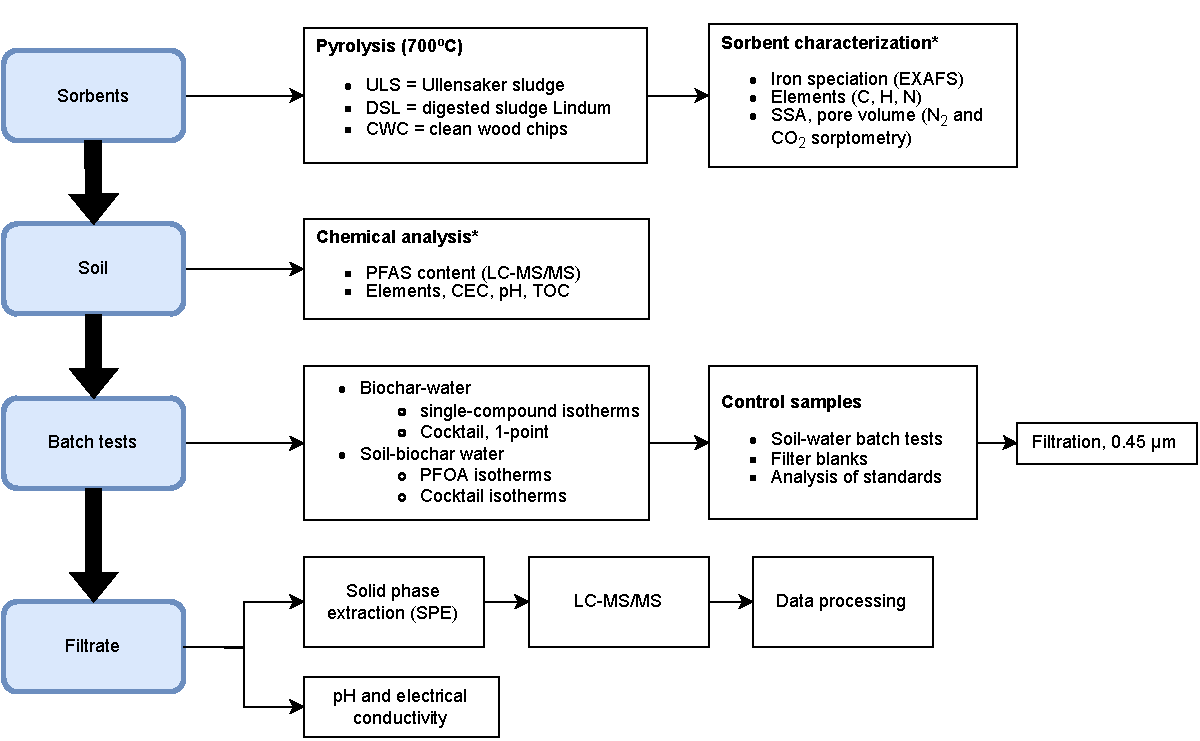
\includegraphics[width=\textwidth]{Diagrams/Methods-General_overview_methods.pdf}
    \caption{Overview of the methods conducted for this thesis. * = analyses conducted by commercial laboratories or that were delegated to project partners.}
    \label{fig:methodoverview}
\end{figure}

\section{Biochar sorbents}

\subsection{Feedstock}
Three feedstock types were selected as sorbents in the sorption experiments: Ullensaker Sludge (ULS), Digested Sludge Lindum (DSL) clean wood chips (CWC). ULS is raw sewage sludge from Ullensaker WWTP that has been dewatered. DSL is sewage sludge that has been through anaerobic digestion (AD) to produce biogas, also referred to as digestate. Anaerobic digestion is performed at Lindum AS and produces methane (and other gases; \cref{eq:AD}) which becomes commercial biogas fuel. The sewage sludge is dewatered, dried and pelletized before pyrolysis. CWC is made of clean, fresh softwood timber without additives that have been shredded, dried, and compressed into 8 mm pellets. The wood pellets are commercially available from Hallingdal trepellets (Kleivi næringspark, Ål).

\subsection{Pyrolysis}
CWC, ULS, and DSL biochars were produced by slow pyrolysis at 700 \textdegree C using ETIA technology by Biogreen\textsuperscript{\textcopyright} at Lindum AS (Drammen, Norway). \cref{tab:sorbents} summarizes the variables for pyrolysis of each biochar. The three biochars were produced as part of a larger study on the life cycle of waste based sorbents and was given as biochar samples to conduct the sorption experiments on for this thesis. The pyrolysis chamber is first electrically heated to stable PT. Feedstock pellets are added to a feeding container (\cref{fig:feeder}) where a heated rotating screw (Spirajoule\textsuperscript{\textregistered}) transports the feedstock into and through the pyrolysis chamber at the programmed RT (\cref{fig:pyrolysischamber}). The biochar is then transported to an external collection container where it is dispensed into sampling bags \cref{fig:biocharCollection}. \cref{fig:pellets} shows the pellets before and after pyrolysis. 

\begin{table}
\centering
\caption{Pyrolysis temperature (PT), residence time (RT) and feedstock for the biochars used in the sorption experiments.}
\label{tab:sorbents}
\begin{tabular}{llll}
\toprule
Biochar   & PT & RT & Feedstock \\
sorbent & (\textdegree C) & (min) \\
\midrule
CWC  & 700 & 20 & clean wood chips  \\
ULS & 700 & 40  & Ullensaker sludge\\
DSL & 700 & 20 & Digested sludge Lindum \\
\bottomrule
\end{tabular}
\end{table}

\begin{figure}
    \centering
    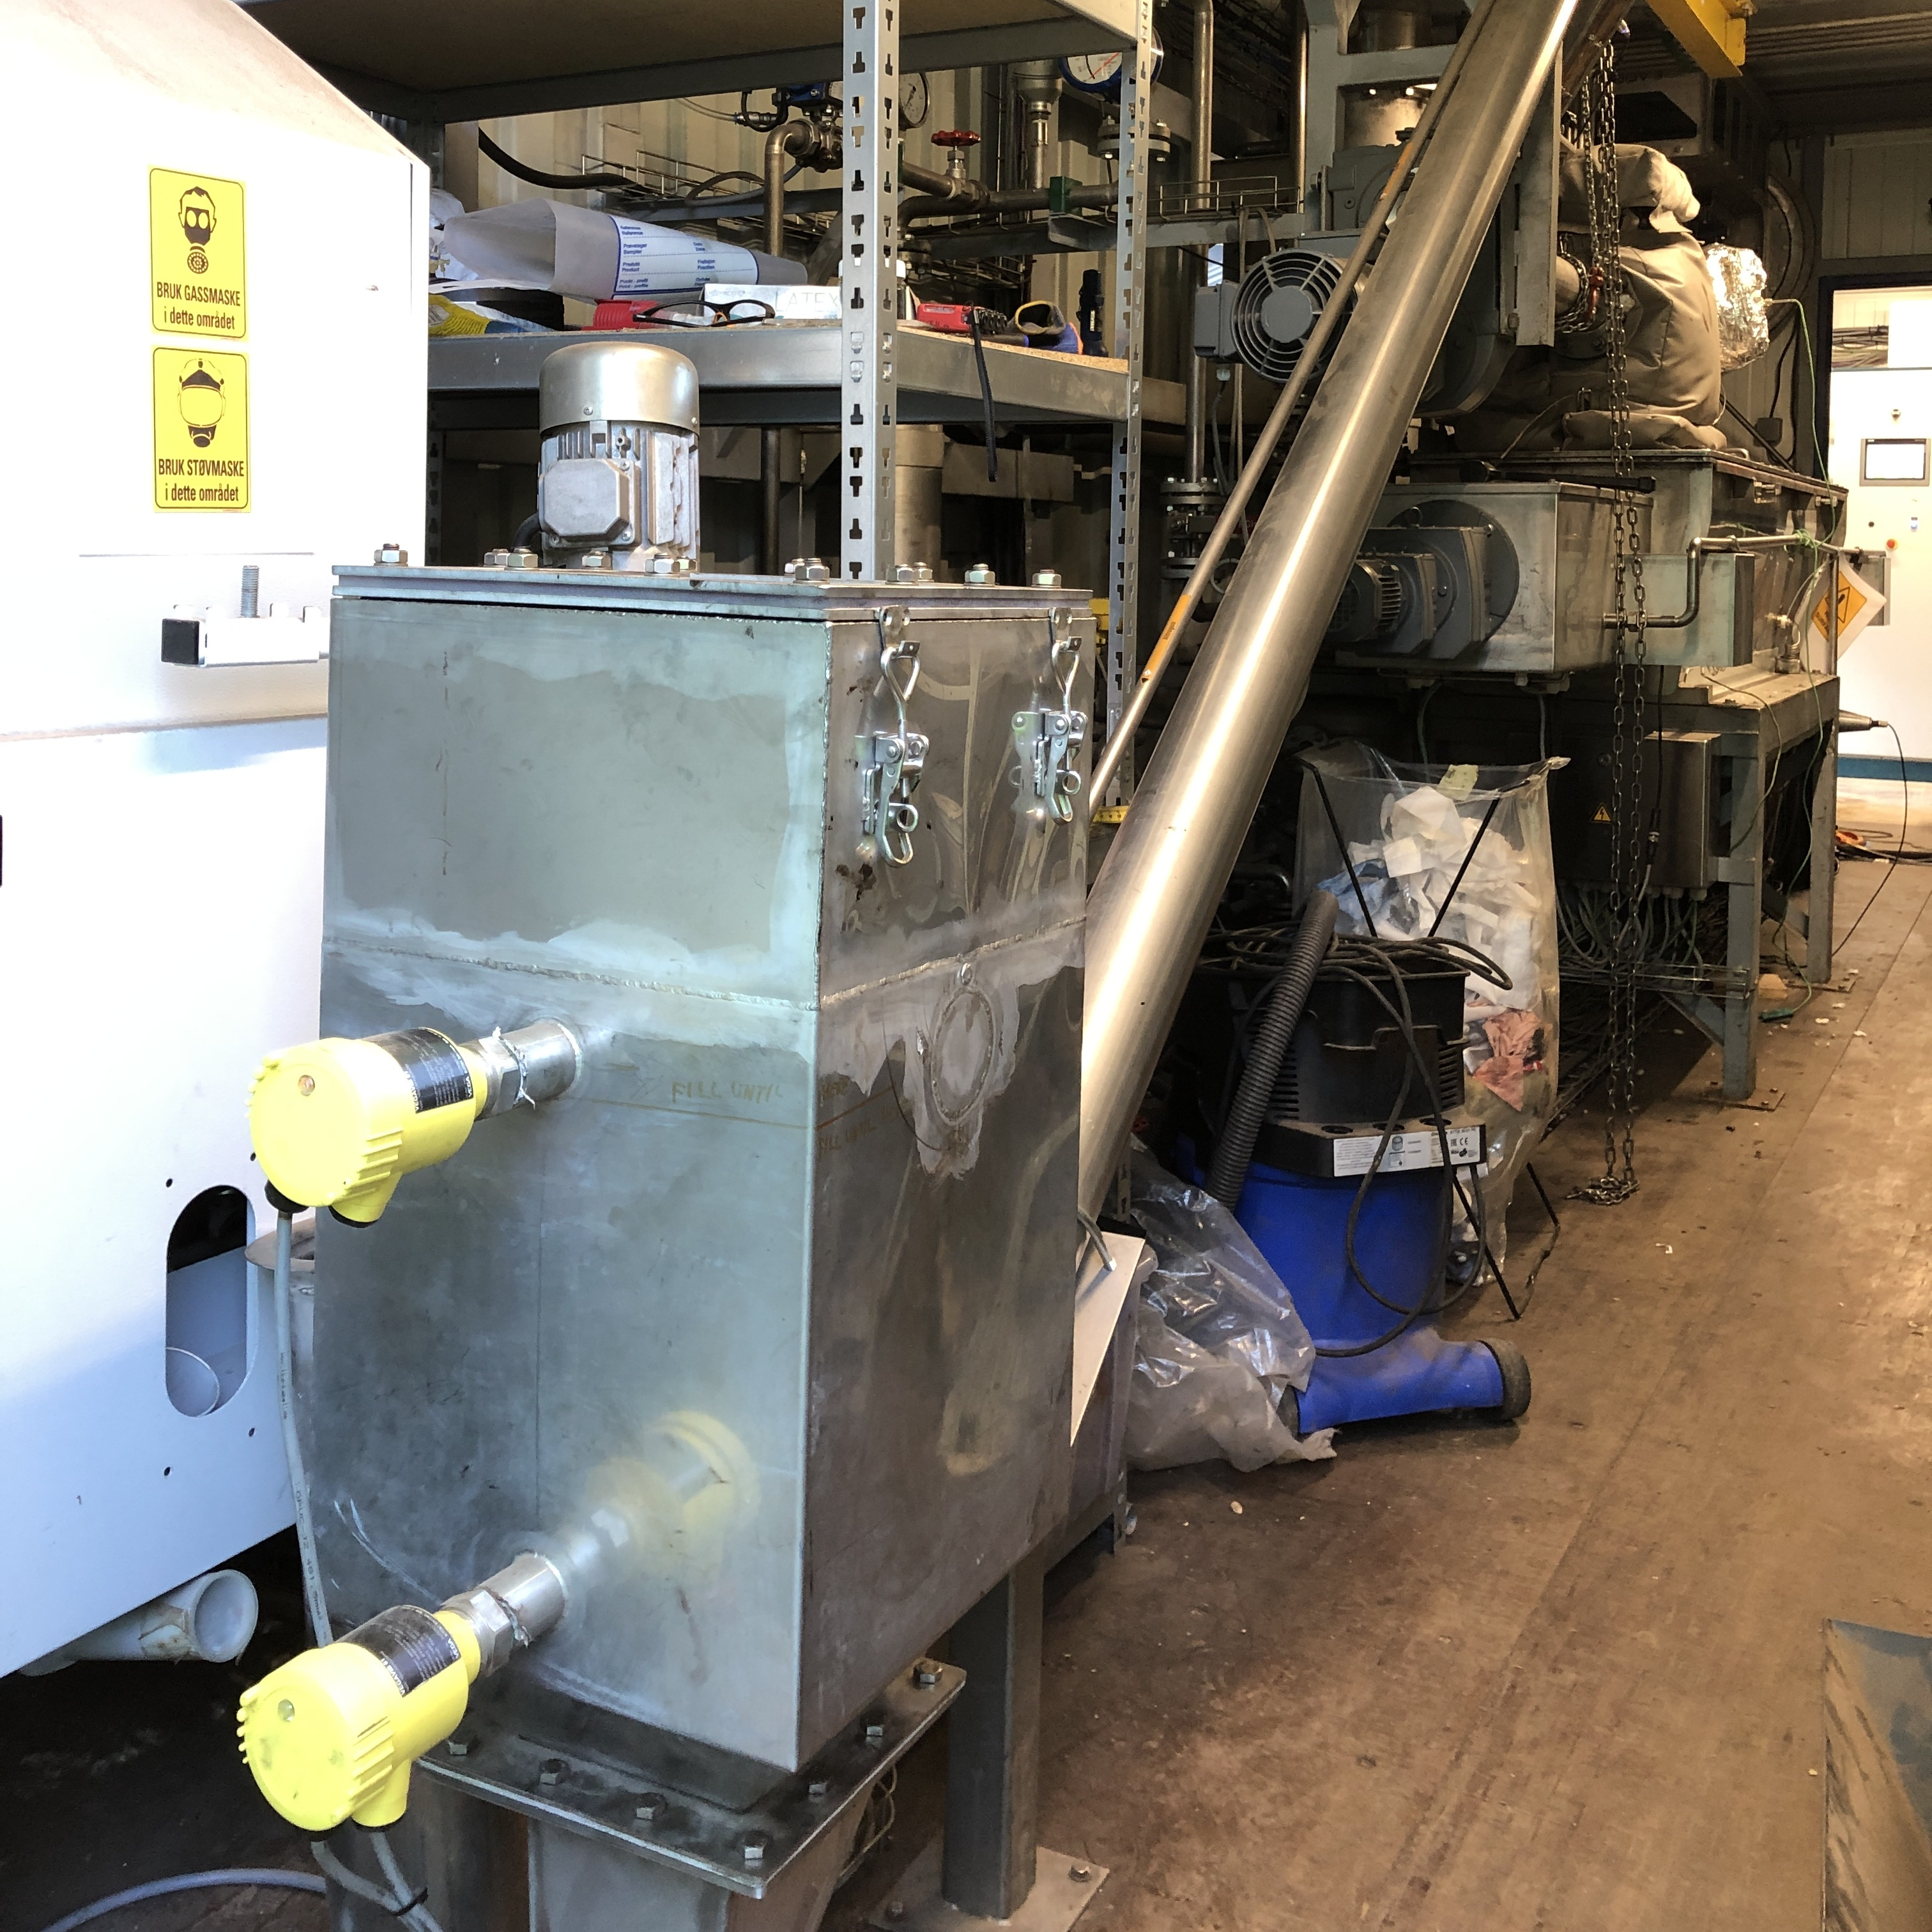
\includegraphics[width=0.6\linewidth,scale=0.6]{Bilder/Pyrolysis/Feeder.jpg}
    \caption{Starting point for the pyrolysis process where feedstock pellets are added to the system and transported with a rotating screw up the pipe on the photo that leads to the pyrolysis chamber.}
    \label{fig:feeder}
\end{figure}

\begin{figure}
    \centering
     \begin{subfigure}[t]{\linewidth}
         \centering
         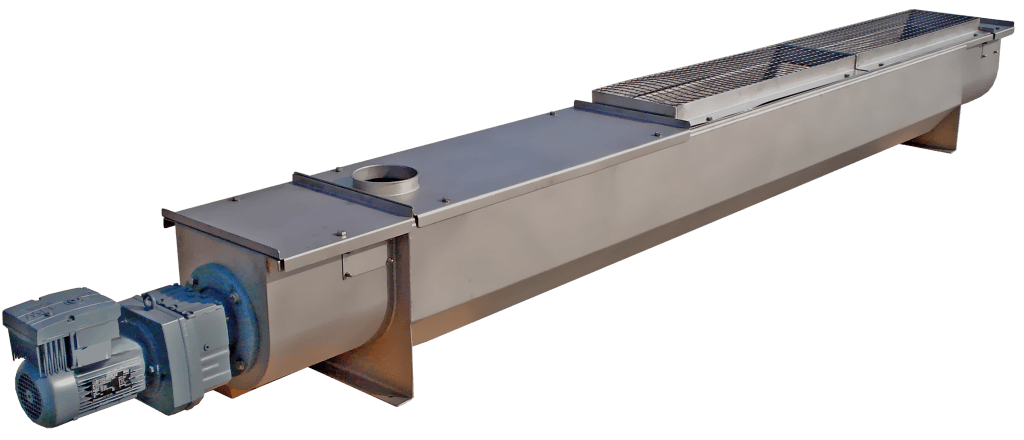
\includegraphics[width=0.74\linewidth,scale=0.74]{Bilder/Pyrolysis/PyrolyzerChamber.png}
         \caption{}
     \end{subfigure}
    \centering
    \begin{subfigure}[b]{\linewidth}
         \centering
         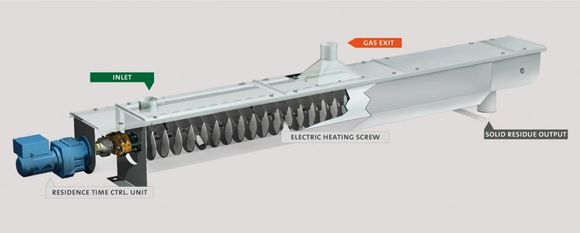
\includegraphics[width=0.74\linewidth,scale=0.74]{Bilder/Pyrolysis/spirajoule.jpeg}
         \caption{}
     \end{subfigure}
    \caption{\textbf{(a)} external view of the pyrolysis chamber, \textbf{(b)} internal view of the pyrolysis chamber. The Spirajoule\textsuperscript{\textregistered} is heated to the desired pyrolysis temperature and the speed of rotation is set to the wanted residence. Adopted from \url{https://www.biogreen-energy.com/spirajoule}.}
    \label{fig:pyrolysischamber}
\end{figure}

\begin{figure}
    \centering
    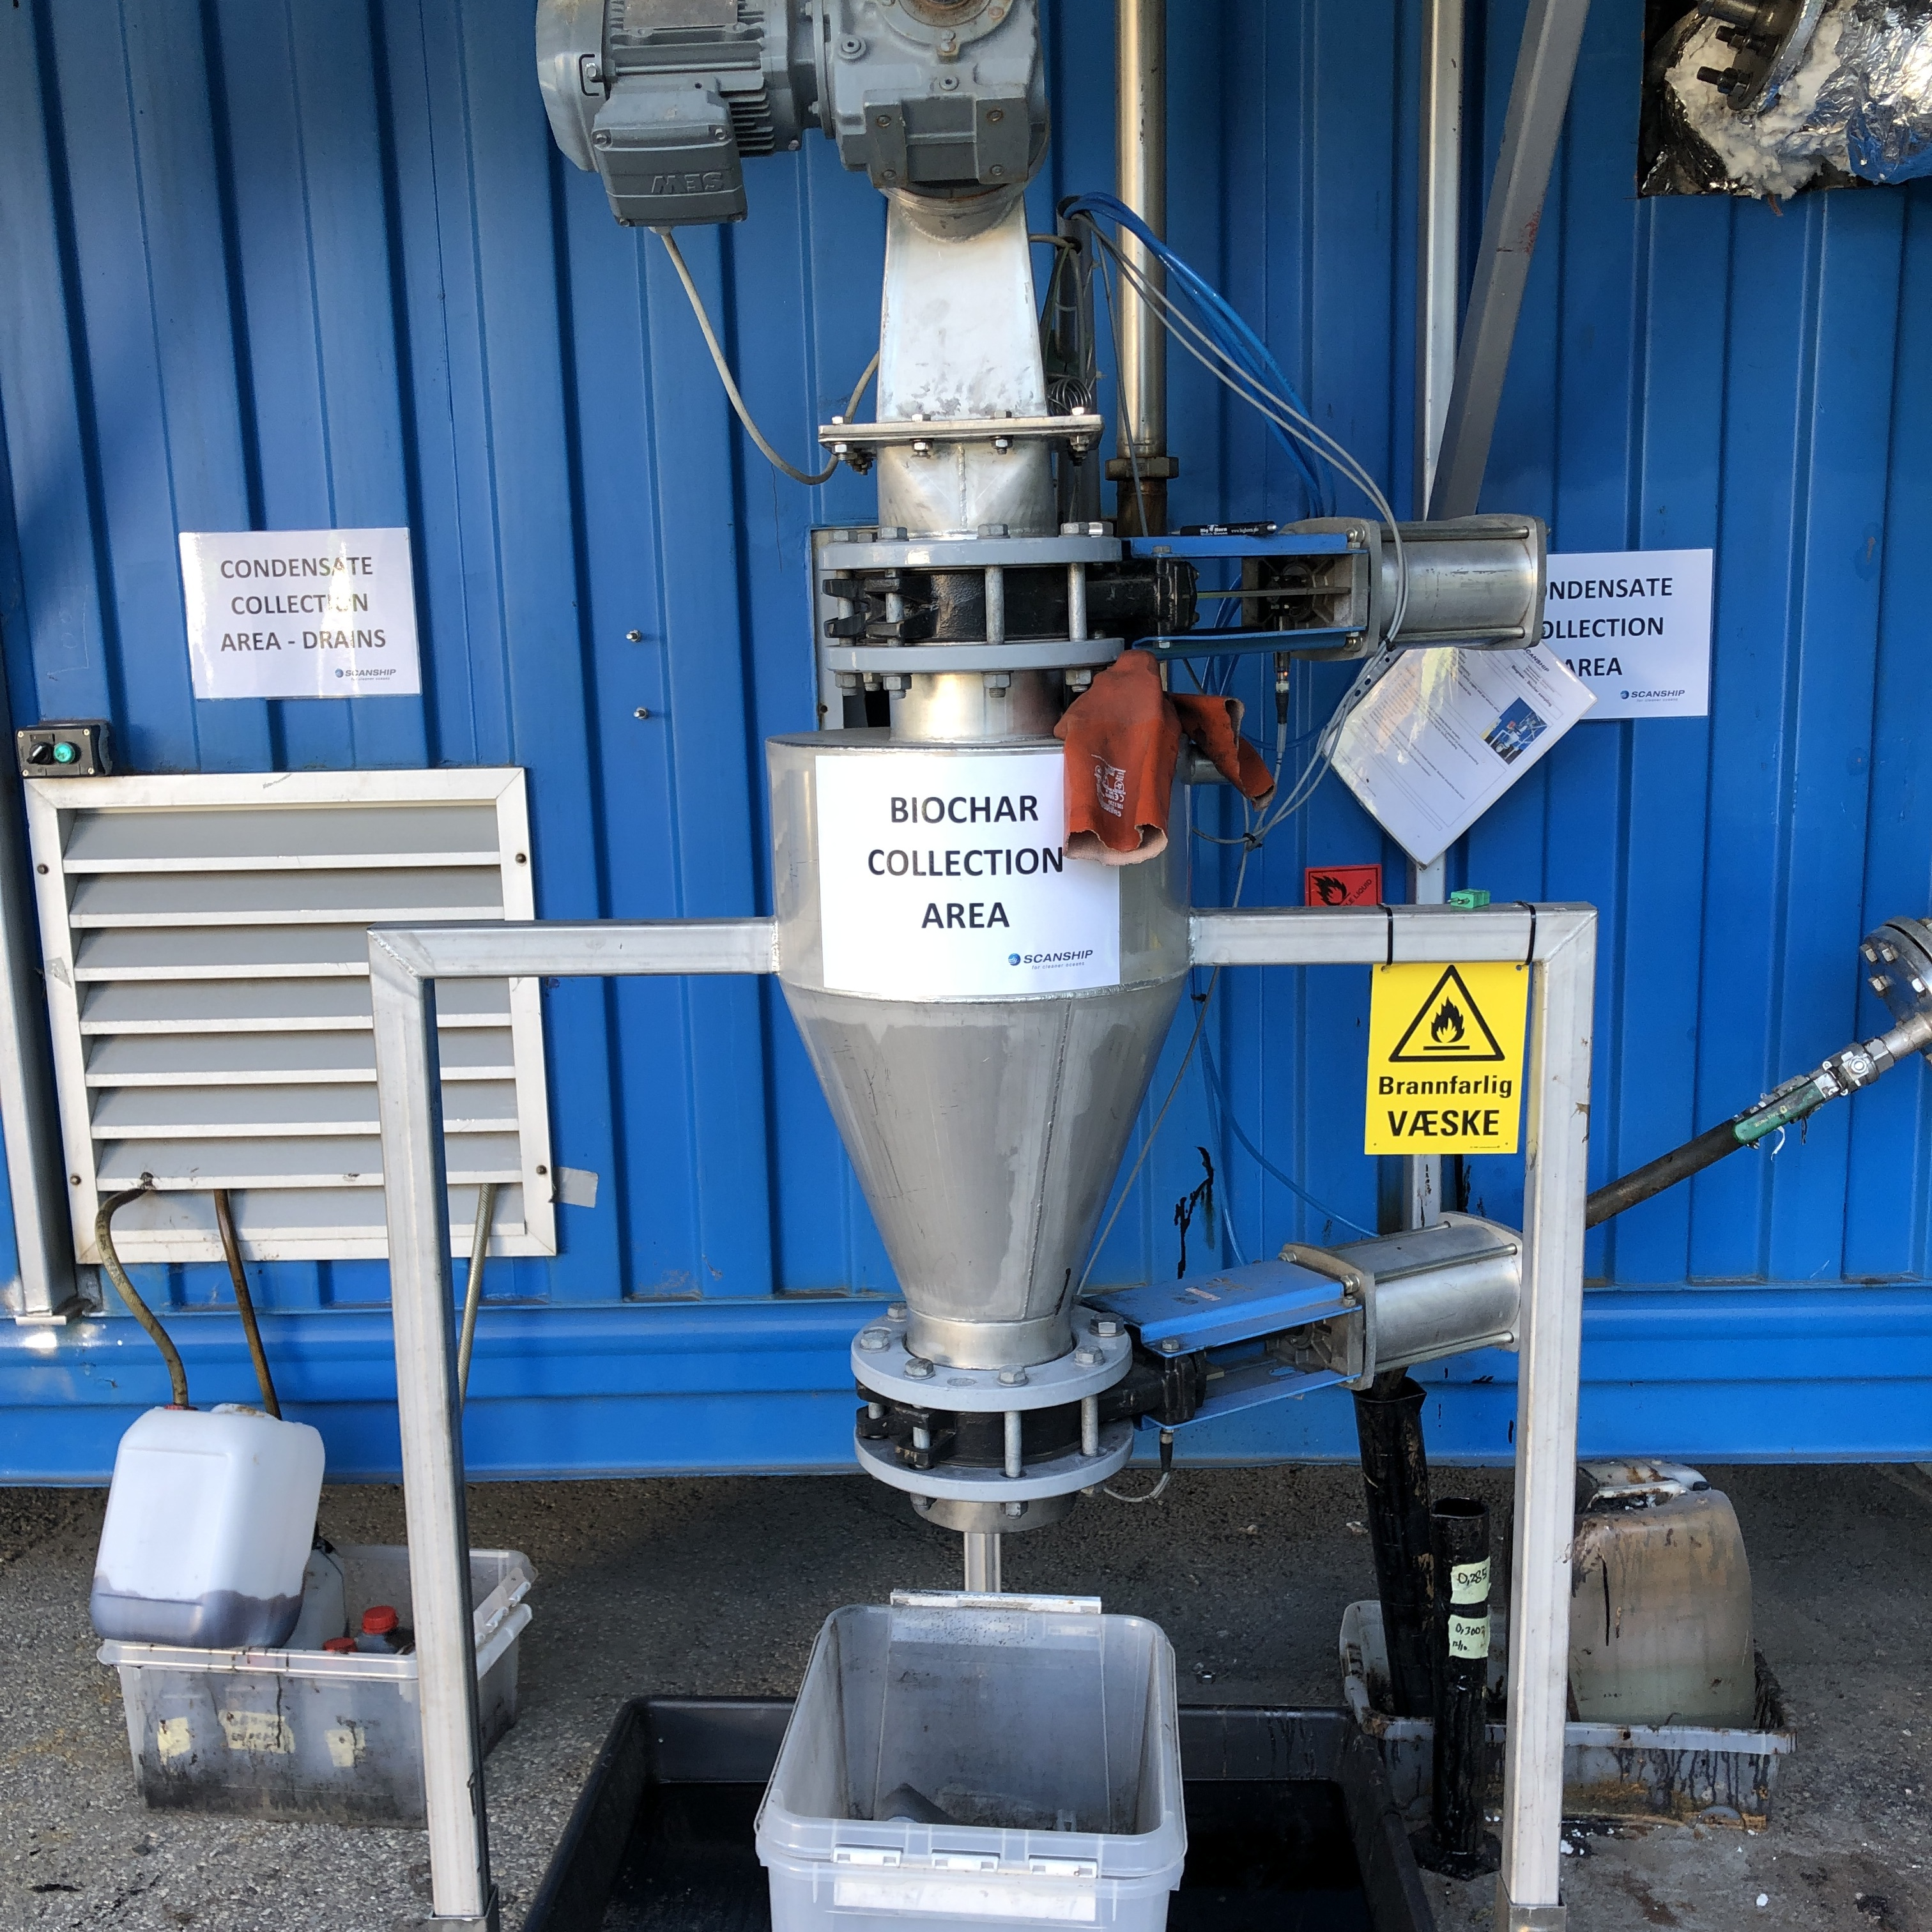
\includegraphics[width=0.6\linewidth,scale=0.6]{Bilder/Pyrolysis/BiocharCollection.jpg}
    \caption{Biochar collection area.}
    \label{fig:biocharCollection}
\end{figure}

\begin{figure}
    \centering
    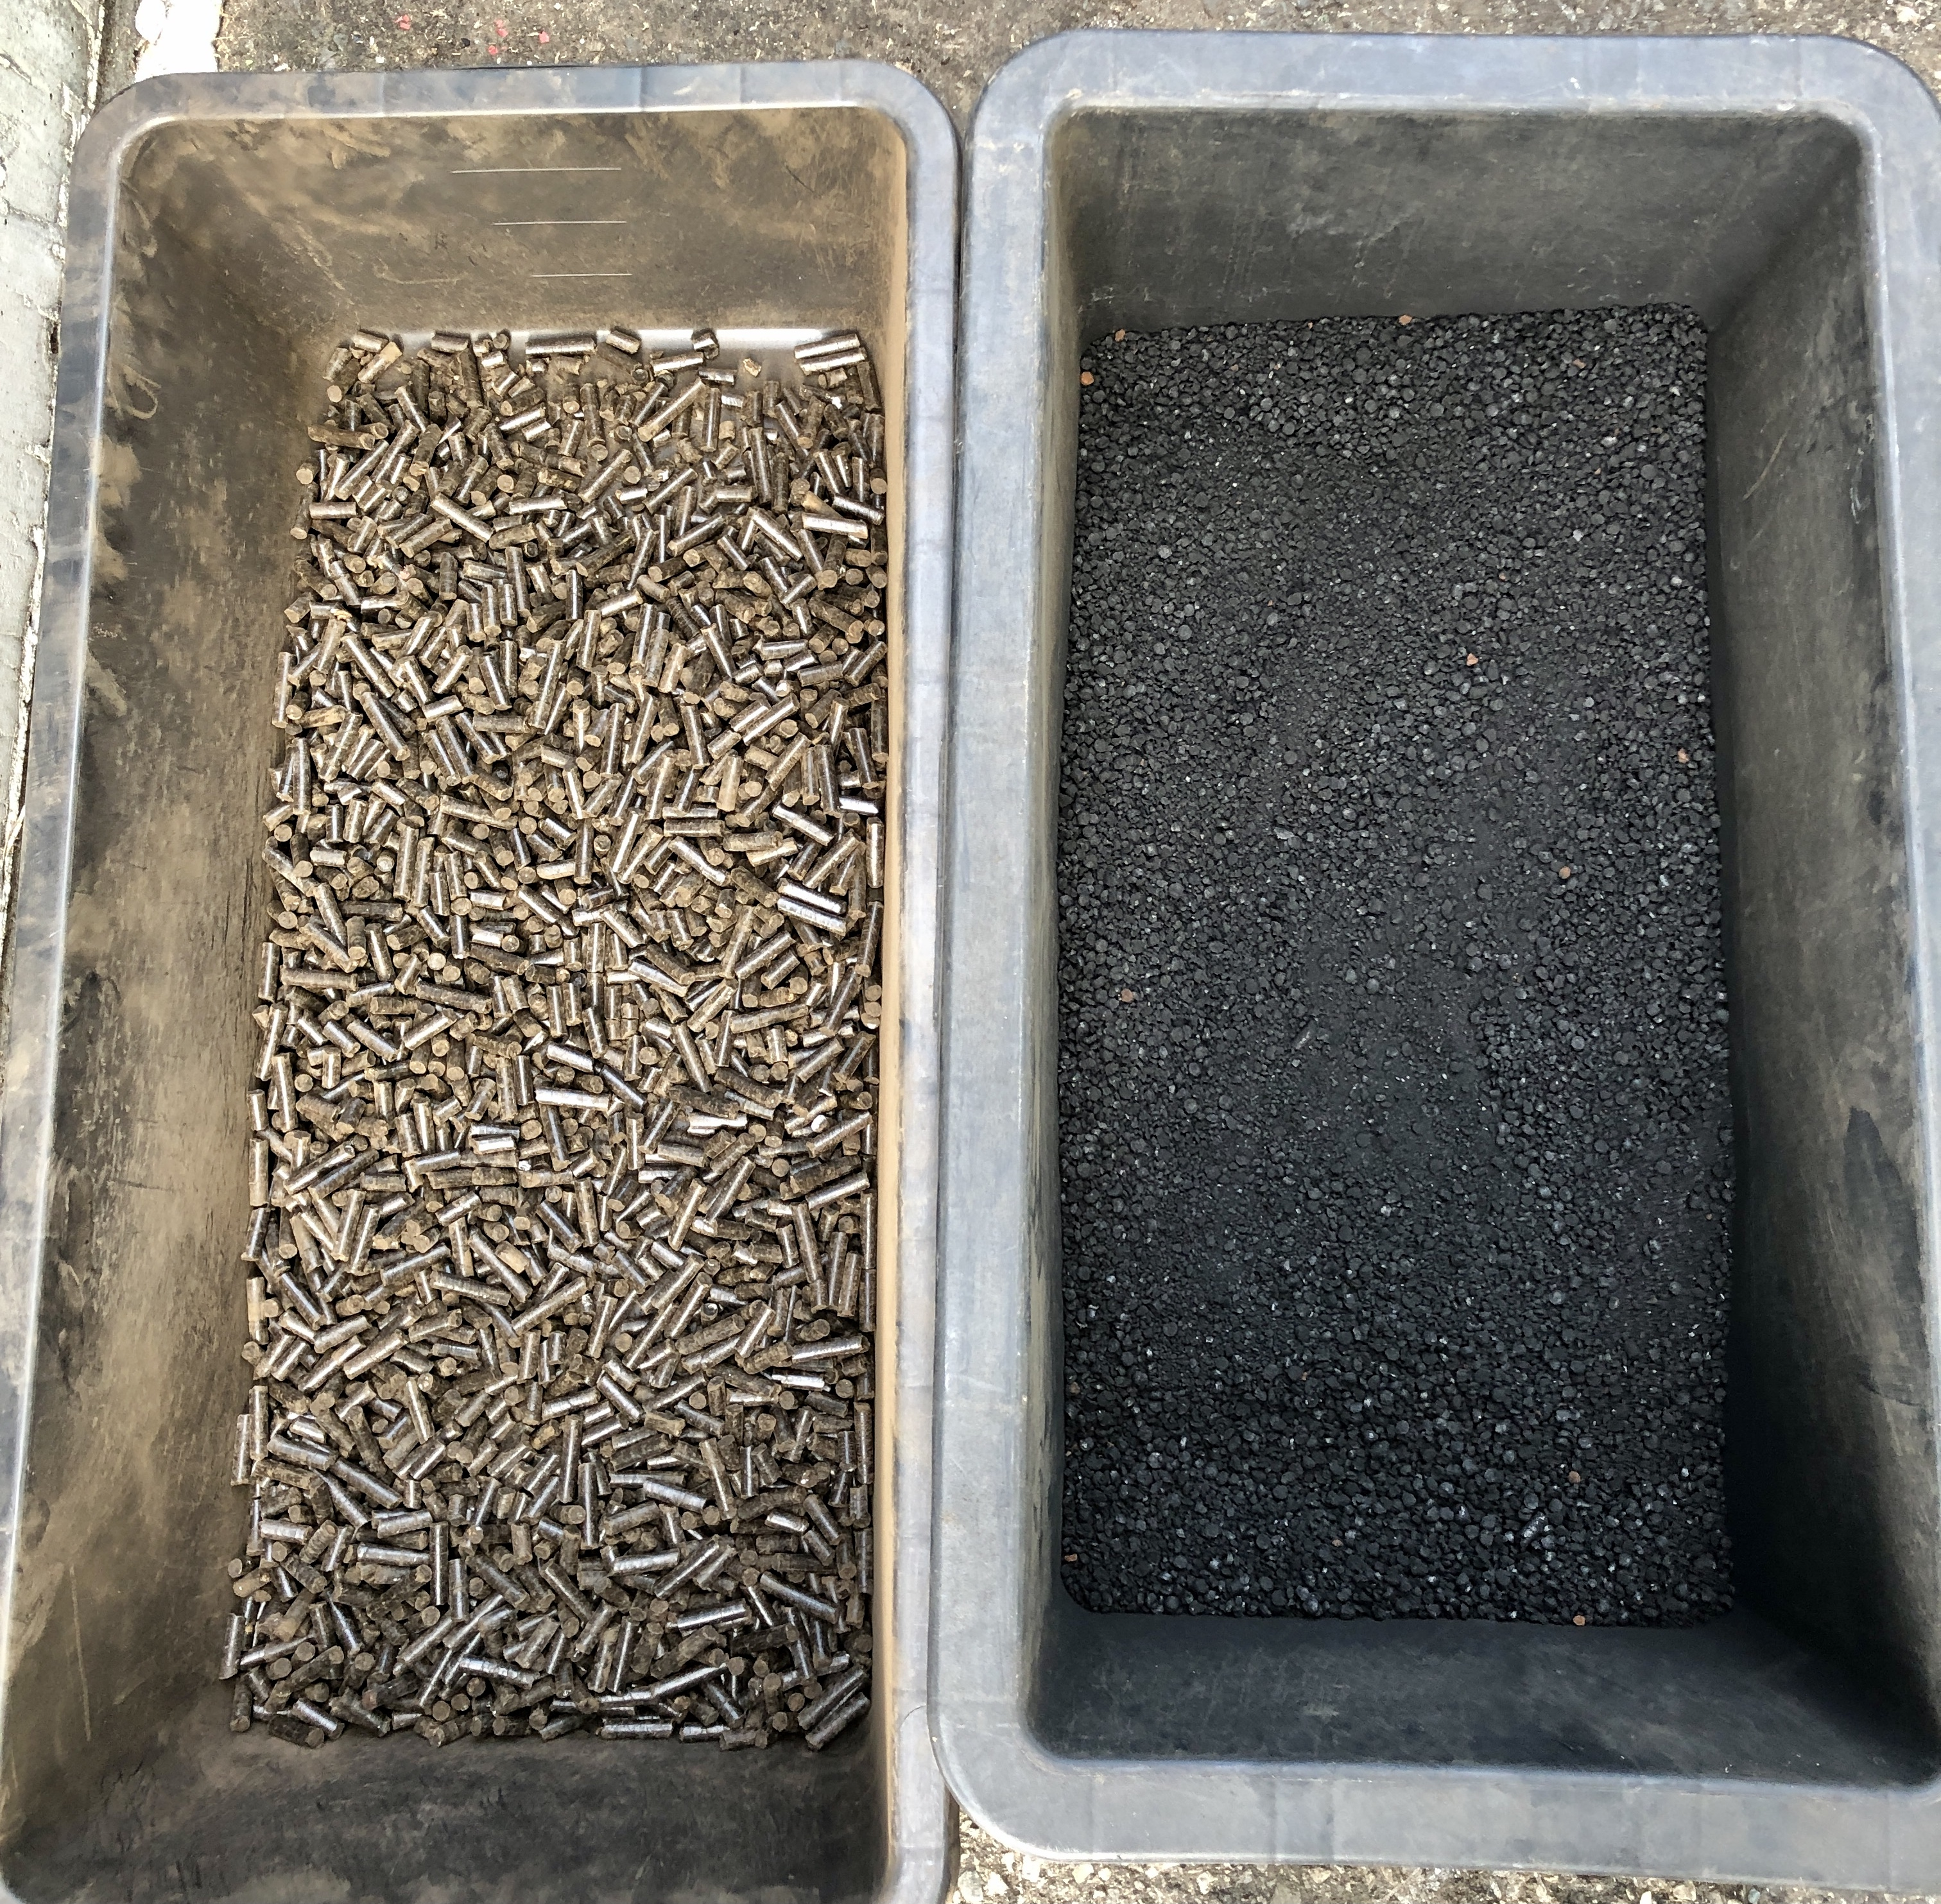
\includegraphics[width=0.6\linewidth,scale=0.6]{Bilder/Pyrolysis/Pellets.png}
    \caption{DSL feedstock pellets (left) and pyrolyzed pellets/biochar (right).}
    \label{fig:pellets}
\end{figure}

Syn-gas from pyrolysis is led through a condensing pipe that condenses into bio-oil at two points depending on boiling point. Syn-gas that does not condense at this point is led into a combustion chamber where a steady inflow of propane ensures a clean burning process of the remaining molecules. See \cref{appSec:pollution} for additional work on measurements on environmental pollutant emission from the ETIA unit.



\subsection{Biochar characterization}

\subsubsection{Surface area and pore volume}
Total specific surface area and pore volume were determined by $\mathrm{N_2}$ and $\mathrm{CO_2}$ gas sorptiometry by research partners at the Particle Engineering Research Center, University of Florida (Gainesville, USA) with a Quantachrome Autosorb 1 surface area analyzer according to the methods described by \cite{kwon2005}.  $\mathrm{N_2}$ sorptiometry was performed at the boiling point for liquid nitrogen (-195.8 \textdegree C). Due to slow diffusion at this low temperature, sorption of  $\mathrm{N_2}$ represents the largest pores of \textgreater 1.5 nm. $\mathrm{CO_2}$ sorptiometry was performed at 0 \textdegree C, and the higher temperature allows the gas to diffuse into smaller pores between 0.4-1.5 nm. $\mathrm{N_2}$ surface area was interpreted using Brunauer, Emmett and Teller (BET) theory, pore size and volume using Barret-Joyner-Halenda (BJH) theory, and $\mathrm{CO_2}$ surface area and pore volume were evaluated using density functional theory (DFT) theory . 

\subsubsection{Element analysis}
Elemental composition (total C, H and N) was performed by $\mathrm{NO_3}$ digestion and quantified with a Leco CHN-1000 from Leco Corporations (Sollentuna, Sweden), according to DIN 51732 by project partner.  

\subsubsection{Iron speciation}
Iron and copper speciation of DSL and ULS were analyzed by Fe K-edge X-ray absorption fine structures (EXAFS) at the synchrotron SOLEIL (Gif-sur-Yvette, France) (beamline SAMBA) by a project colleague at NGI. To prepare the biochars for analysis, each sample ($\sim$50 mg) was crushed with a mortar to a fine powder (250 \textmu m). The samples were mixed with boron nitride (BN, 300 mg) to a homogeneous powder and pelletized. BN matrix is used for sample dilution because it absorbs very little of the photon beam at the Fe K-edge. The biochar pellet was then analyzed by X-ray absorption spectroscopy.  

The overall principle of EXAFS is to determine structural composition of a sample by examining its X-ray absorption spectrum, which plots absorbance, $\mu x$, as a function of photon energy, $eV$ \citep{vlaica2004exafs}. The sample is submitted to an X-ray beam where a spectrophotometer measures the beam intensity going through the sample. The difference of intensity between before and after the sample is translated into an absorption coefficient, following Beer-Lambert's Law: 

\begin{equation}\label{eq:absorbance}
    \mu x = log \frac{I}{I_0}
\end{equation}

where $\mu x$ is a dimensionless absorbance coefficient ($AU$), $I$ is the transmitted light intensity and $I_0$ is the incident light intensity. The energy of the photon beam is determined by the angle of a crystal monochromator. The angle of the crystal monochromator is tuned so that the sample is submitted to a range of photon energies in which the absorption edges of the target element lie within \citep{vlaica2004exafs}. An adsorption K-edge occurs when the transmitted photon energy equals the energy required to excite a core electron, which is observed as a vertical jump (K) in $\mu x$ on the spectrum \citep{vlaica2004exafs}. The neighboring elements are interfering with the photon wave, which translates into oscillations on the absorption spectrum following the absorption edge. Each element has a different retrodiffusion coefficient, therefore the frequency and amplitude of oscillations in the absorption spectrum are (partially) determined by the type and number of neighboring atoms. The absorption edge energy and the oscillations thus contain information on the valency of the element and number and type of neighboring atoms, i.e., the element speciation. Fe(II) species will have K at a lower energy than Fe(III) species because a higher photon energy is required to excite an electron from the more electronegative Fe(III). In addition, the oscillations will differ depending on the Fe mineral. By interpreting the X-ray absorption spectrum, the different iron species present in the sample can be derived.

%%%%%%%%%%%%%%%%%%%%%%%%%%%%%%%%%%%%%%%%%%%%%%%%%%%%%%%%%%%%%%%%%%%%%%%%%%%%%%%%%%%%%%%%%%%%%%%%%%%%%%%%%%%%%%%

\section{Sorption experiments}
Effectiveness of PFCA removal by waste biochar was evaluated by batch shaking tests. The following section describes how the batch tests were prepared.

\subsection{Experiment preparations}
\subsubsection{Target compounds}\label{sec:PFCAanalytic}
Six perfluorinated carboxylic acids (PFCAs): perfluoropentanoic acid (PFPeA), perfluorohexanoic acid (PFHxA), perfluoroheptanoic acid (PFHpA), perfluorooctanoic acid (PFOA), perfluorononaoic acid (PFNA), perfluorodecanoic acid (PFDA), with perfluorinated carbon (PFC) units 4-9 respectively were chosen as sorbates for the batch test experiments in this thesis. Hereafter, these are referred to as target compounds/TCs. See \cref{tab:PFCAs} for a list of all native PFCAs including their respective CAS numbers included in this thesis. 10 mL stock solutions were prepared for each TC by weighing the pure PFCA salts/liquid (\cref{tab:PFCAs}) on an analytical scale and dissolving them in methanol in volumetric flasks. Two spiking standards at a high (STD1) and low (STD2) concentration were prepared from the stock solution to be used for spiking the batch tests at various concentrations (\cref{apptab:standards}). The working standards were analyzed with LC-MS/MS of a 2-time diluted standard at an optimum concentration for the instrument calibration curve (10-20 \textmu g L\textsuperscript{-1}, \cref{appSec:IsothermSetup}) and all further calculations of spike dilutions were corrected with the measured standard concentrations.

\begin{table}
\centering
\caption{PFAS compounds investigated in this study. PFCs correspond to the number of perfluorinated carbon units in the chain. Note: PFCAs appear in dissociated form at environmentally relevant pH's due to low $pK_a$'s.}
\adjustbox{max width=\textwidth}{
\label{tab:PFCAs}
\begin{tabular}{@{}lcccclc@{}}
\toprule
\multicolumn{1}{c}{Chemical} & Acronym & Short & CAS number & Molecular structure & Stock form & Purity \\ \midrule
& & & & & &\\
\smash{\raisebox{4ex}{Perfluoropentanoic acid}}  & \smash{\raisebox{4ex}{PFPeA}} & \smash{\raisebox{4ex}{C5}} & \smash{\raisebox{4ex}{2706-90-3}} & \chemfig[atom style={scale=0.4}]{O=[:90](-[:30,,,1]OH)-[:150](-[:112.5]F)(-[:67.5]F)-[:210](-[:292.5]F)(-[:247.5]F)-[:150](-[:112.5]F)(-[:67.5]F)-[:210](-[:270]F)(-[:150]F)-[:210]F} & \smash{\raisebox{4ex}{liquid}} & \smash{\raisebox{4ex}{\textgreater 97 \%}} \\
& & & & & &\\
\smash{\raisebox{4ex}{Perfluorohexanoic acid}} & \smash{\raisebox{4ex}{PFHxA}}  & \smash{\raisebox{4ex}{C6}} & \smash{\raisebox{4ex}{307-24-4}} & \chemfig[atom style={scale=0.4}]{O=[:90](-[:30,,,1]OH)-[:150](-[:112.5]F)(-[:67.5]F)-[:210](-[:292.5]F)(-[:247.5]F)-[:150](-[:112.5]F)(-[:67.5]F)-[:210](-[:292.5]F)(-[:247.5]F)-[:150](-[:210]F)(-[:150]F)-[:90]F} & \smash{\raisebox{4ex}{liquid}} & \smash{\raisebox{4ex}{\textgreater 97 \%}} \\
& & & & & &\\
\smash{\raisebox{4ex}{Perfluoroheptanoic acid}} & \smash{\raisebox{4ex}{PFHpA}} & \smash{\raisebox{4ex}{C7}} & \smash{\raisebox{4ex}{375-85-9}} & \chemfig[atom style={scale=0.4}]{O=[:90](-[:30,,,1]OH)-[:150](-[:67.5]F)(-[:112.5]F)-[:210](-[:247.5]F)(-[:292.5]F)-[:150](-[:67.5]F)(-[:112.5]F)-[:210](-[:247.5]F)(-[:292.5]F)-[:150](-[:67.5]F)(-[:112.5]F)-[:210](-[:150]F)(-[:210]F)-[:270]F} & \smash{\raisebox{4ex}{crystalline}} & \smash{\raisebox{4ex}{\textgreater 99 \%}} \\
& & & & & &\\
\smash{\raisebox{4ex}{Perfluorooctanoic acid}} & \smash{\raisebox{4ex}{PFOA}}  & \smash{\raisebox{4ex}{C8}} & \smash{\raisebox{4ex}{335-76-2}}  & \chemfig[atom style={scale=0.4}]{O=[:90](-[:30,,,1]OH)-[:150](-[:67.5]F)(-[:112.5]F)-[:210](-[:247.5]F)(-[:292.5]F)-[:150](-[:67.5]F)(-[:112.5]F)-[:210](-[:247.5]F)(-[:292.5]F)-[:150](-[:67.5]F)(-[:112.5]F)-[:210](-[:247.5]F)(-[:292.5]F)-[:150](-[:90]F)(-[:150]F)-[:210]F} & \smash{\raisebox{4ex}{powder}} & \smash{\raisebox{4ex}{\textgreater 95 \%}} \\
& & & & & &\\
\smash{\raisebox{4ex}{Perfluorononaoic acid}}  & \smash{\raisebox{4ex}{PFNA}} & \smash{\raisebox{4ex}{C9}} & \smash{\raisebox{4ex}{375-95-1}} & \chemfig[atom style={scale=0.4}]{O=[:90](-[:30,,,1]OH)-[:150](-[:112.5]F)(-[:67.5]F)-[:210](-[:292.5]F)(-[:247.5]F)-[:150](-[:112.5]F)(-[:67.5]F)-[:210](-[:292.5])(-[:247.5]F)-[:150](-[:112.5]F)(-[:67.5]F)-[:210](-[:292.5]F)(-[:247.5]F)-[:150](-[:112.5]F)(-[:67.5]F)-[:210](-[:270]F)(-[:210]F)-[:150]F} & \smash{\raisebox{4ex}{crystalline}} & \smash{\raisebox{4ex}{\textgreater 97 \%}} \\
& & & & & &\\
\smash{\raisebox{4ex}{Perfluorodecanoic acid}}  & \smash{\raisebox{4ex}{PFDA}}  & \smash{\raisebox{4ex}{C10}} & \smash{\raisebox{4ex}{335-67-1}} & \chemfig[atom style={scale=0.4}]{O=[:90](-[:30,,,1]OH)-[:150](-[:112.5]F)(-[:67.5]F)-[:210](-[:292.5]F)(-[:247.5]F)-[:150](-[:112.5]F)(-[:67.5]F)-[:210](-[:292.5]F)(-[:247.5]F)-[:150](-[:112.5]F)(-[:67.5]F)-[:210](-[:292.5]F)(-[:247.5]F)-[:150](-[:112.5]F)(-[:67.5]F)-[:210](-[:292.5]F)(-[:247.5]F)-[:150](-[:210]F)(-[:150]F)-[:90]F} & \smash{\raisebox{4ex}{flakes}} & \smash{\raisebox{4ex}{\textgreater 98\%}} \\
& & & & & &\\ \bottomrule
\end{tabular}}
\end{table}

\subsubsection{Spike concentrations}
A final concentration interval over four orders of magnitude where the lowest concentration point lies close to the instrumental LOQs was desired in order to provide sorption isotherms that spans both the regions of linear sorption and sorption attenuation according to the Freundlich sorption model. To achieve detectable concentrations across this range, determination of appropriate spike concentrations was based on several factors: 1) Biochar-water partition coefficients ($K_{BC}$) for the TCs obtained from literature \cite{Xiao2017} \cref{tab:Kbc}, 2) biochar dose, 3), the LOQ of the analytical method for, and 4) available pipetting volume range. 

The relationship between $K_{BC}~\mathrm{(L~g^{-1})}$, the sorbed concentration, $C_s~\mathrm{(\mu g~g^{-1})}$, and the freely dissolved aqueous concentration, $C_w~\mathrm{(\mu g~L^{-1})}$, expressed as:

\begin{align}
    \label{eq:Kbc1}
    K_{D} = \frac{C_s}{C_w}
\end{align}

was used to estimate the expected $C_w$. By rearranging \cref{eq:Kbc1},  $C_w$ is expressed as a function of the mass TA spiked and the estimated $K_D$:

\begin{align}
    \label{eq:Cw2}
    C_w=\frac{\frac{m_{PFAS}}{\left (\frac{m_{BC}\times K_{BC}}{V_w}\right)+1}}{V_w}
\end{align}

Where $m_{TA}$ is the mass PFAS spiked, $m_{BC}$ is the biochar dose, and $V_w$ is the volume of the sample matrix. Using \cref{eq:Cw2}, the lowest spike concentration for each isotherm was taken to be two times the method LOQ for the LC-MS/MS instrument at NTNU, Trondheim (\cref{apptab:LOQ}). The remaining points were spread evenly over a $10^4$ concentration interval. 

\begin{table}
\centering
\caption{Biochar-water distribution coefficients ($K_{BC}$) for PFCAs derived from \cite{XiaoSI2017}.} 
\label{tab:Kbc}
\begin{threeparttable}
    \begin{tabular}{@{}lcc@{}}
    \toprule
    \multicolumn{1}{l}{\begin{tabular}[l]{@{}l@{}}Compound\end{tabular}} &  \multicolumn{1}{c}{\begin{tabular}[c]{@{}c@{}}log $\mathrm{K_{BC}}$\\ \citep{XiaoSI2017}\end{tabular}} & \multicolumn{1}{c}{\begin{tabular}[c]{@{}c@{}}est. log $\mathrm{K_{BC}}$ \end{tabular}} \\ \midrule
    PFPeA & 4.16 & 4.16 \\
    PFHxA & 4.15 & 4.15 \\
    PFHpA & 4.49 & 4.49 \\
    PFOA & 4.76 & 4.76 \\
    PFNA & *4.89 & 4.89 \\
    PFDA & *5.09 & 5.09 \\ \bottomrule             
    \end{tabular}
\begin{tablenotes}
\item * not included in \citep{XiaoSI2017}, so the values are extrapolated from the shorter chain lengths.
\end{tablenotes}
\end{threeparttable}
\end{table}

Two preliminary batch tests were prepared to check how well the $K_d$ values selected from the literature corresponded to those for ULS and CWC. Further details about this analysis are provided in \cref{appSec:IsothermSetup}.

\subsubsection{Biochar}
A sub sample (100 g) was taken by random grab sampling from the bulk volume of the biochar produced during the pyrolysis run. The biochars were crushed using a ball mill (Retsch ISO 9001) with five balls at 50 rpm for 5 minutes and sieved into fine-powdered biochar (D \textless 1 mm) and transferred to LDPE zipper bags for storage (4 \textdegree C). 

\subsubsection{Soil}
The soil used for the sorption tests was an unaged sandy soil obtained from a remote field area 17 km from Uppsala, Sweden (59.733 N, 17.667 E). TOC-content was determined according to... pH according to... The soil was characterized for total element concentrations, exchangeable ions, TOC and pH by... the methods... The soil was dried at 100 \textdegree C for 24 h and crushed and sieved to \textless 2 mm.  The soil was screened for PFAS using a methanol extraction, solid phase extraction and quantification by liquid chromatography coupled with tandem mass spectrometry at NTNU (Trondheim, Norway) by a project partner (details for the SPE and LC-MS/MS procedures will be given in \cref{methods:instrAnalysis}), performed in triplicate.

\begin{figure}
    \centering
    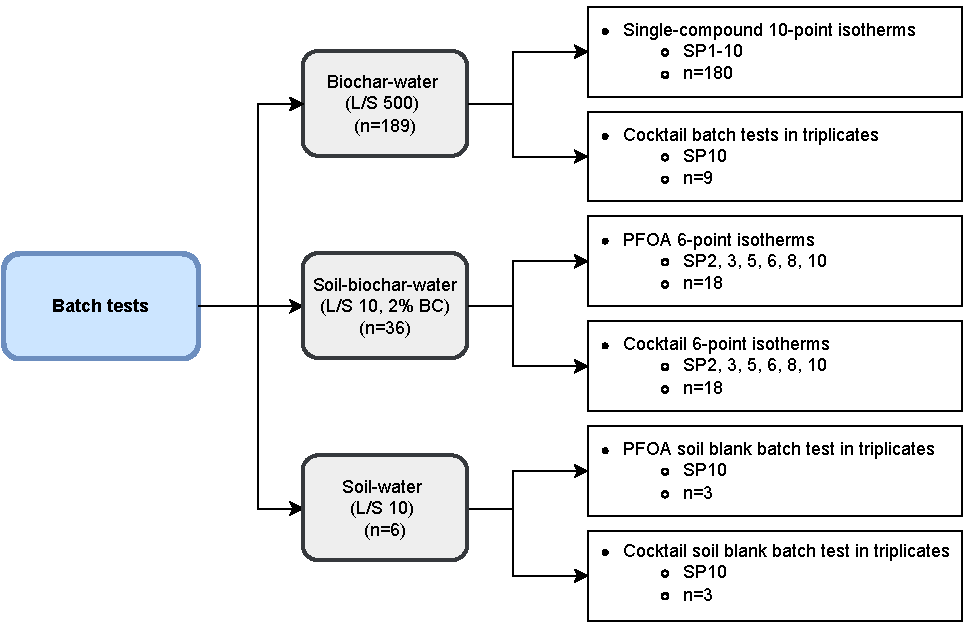
\includegraphics{Diagrams/Methods-Page-9.pdf}
    \caption{Overview of batch test samples for this thesis for the three biochars (ULS, DSL, CWC) and six TCs.}
    \label{fig:batchtests}
\end{figure}

\begin{table}
    \caption{Spike concentrations (SC) in \textmu g L\textsuperscript{-1} used for the batch tests. MIX = cocktail spike concentration for biochar-water batch tests in triplicates, MIX-S = cocktail spike concentration for biochar-soil-water and soil-water batch tests.}
    \label{tab:spikeConcentrations}
    \adjustbox{max width=\textwidth}{%
    \begin{tabular}{lrrrrrrrrrrrr}
    \toprule
    \textbf{Compound} & \textbf{SC1} & \textbf{SC2} & \textbf{SC3} & \textbf{SC4} & \textbf{SC5} & \textbf{SC6} & \textbf{SC7} & \textbf{SC8} & \textbf{SC9} & \textbf{SC10} & \textbf{SC10-MIX} & \textbf{SC10-MIX-S} \\ \midrule
    PFPeA & 0.019 & 21 & 43 & 64 & 86 & 107 & 128 & 150 & 171 & 191 & 191 & 283\\
    PFHxA & 0.033 & 37 & 73 & 110 & 146 & 184 & 220 & 256 & 292 & 330 & 330 & 836 \\
    PFHpA & 0.012 & 11 & 25 & 38 & 52 & 65 & 79 & 92 & 106 & 117 & 117 & 153\\
    PFOA & 0.195 & 216 & 435 & 651 & 871 & 1 087 & 1 302 & 1 522 & 1 742 & 1 953 & 1 953 & 1 974\\
    PFNA & 0.141 & 156 & 313 & 471 & 625 & 784 & 942 & 1 097 & 1 255 & 1 409 & 1 409 & 2 310\\
    PFDA & 0.383 & 425 & 850 & 1 275 & 1 700 & 2 126 & 2 551 & 2 976 & 3 401 & 3 830 & 3 830 & 5 288\\ \bottomrule
    \end{tabular}}
\end{table}

\subsection{Batch tests}
An overview of the experimental setup for the batch test is given in \cref{fig:batchtests}. Details for the preparations of each batch test category are given in the subsections below. The batch tests were prepared with a liquid to solid mass ratio (L/S) of 500 for biochar and L/S of 10 for soil amended with 2\% biochar in accordance with CEN EN 12457. The dry matter was added to pre-cleaned 50 mL PP centrifuge tubes and spiked with either individual PFCAs or a cocktail of all six TCs at the concentrations specified in \cref{tab:spikeConcentrations} to a final liquid volume of 50 mL. The standard concentrations were analytically verified to ensure accuracy of the data analysis (see \cref{appSec:IsothermSetup} for expected vs. analytical concentrations). The samples were assured to contain \textless 10\% MeOH, which is the upper limit for which methanol does not influence sorption (reference). The batch tests were shaken end-over-end (9 rpm) and/or agitated on a shaking table (160 rpm) in room temperature (20\textdegree C) for at least 14 days to reach equilibrium \citep{higgins2006sorption} before filtration through a 0.45 \textmu m Minisart\textsuperscript{\textregistered} regenerated cellulose syringe filter into PP tubes based on the methods described in \cite{Sorengard2019}. Loss of biochar to the walls of the syringe was quantified to maintain a full mass balance when analyzing the partitioning of the TCs between the solid and liquid phase and is in \cref{appSec:misclab}. Therefore, a 100\% mass balance was assumed when calculating partitioning between sorbent and water by subtracting the initial spike concentration from the measured concentration in the filtrates. by also correcting for loss to laboratory ware (reference). 

\subsubsection{Biochar-water batch tests}
100\textpm 4 mg biochar was weighed for the biochar-water batch tests. on an analytical scale and placed into pre-cleaned (50\% methanol) 50 mL PP tubes. The tubes were filled half up of Milli-Q water. In each tube, stock PFCA was pipetted using micro- (5-50 {\textmu}l and 200-1000 {\textmu}L) and milli pipettes (2-10 mL) into the char-water solution to make 10 dilutions for each of the 6 PFCAs in even intervals within the concentration points in \cref{tab:spikeConcentrations}. Some tubes were added Milli-Q water up to the 50 mL mark and some were weighed in order to control for the water amount being within \textpm 0.02 mL. The same ten concentrations were used to spike CWC, ULS and DSL batch tests. A cocktail batch test was prepared for the three biochars at SP10  The same dose biochar was used as for the other sorption isotherms. The cumulative CMC (critical micelle concentration) for the six PFCAs at SC10 was assured not to be an issue for the concentration range considered \citep{bhhatarai2011}.

\subsubsection{Soil-biochar-water batch tests}
5\textpm 0.005 g soil, 0.1\textpm 0.0004 g biochar
The batch tests were prepared as 6-point isotherms within a 10\textsuperscript{4} concentration range with a L/S ratio of 10 in PP tubes, in accordance with CEN EN 12457 with modifications described in \citep{Hale2017fire,Kupryianchyk2016a}. L/S 10  is common in leaching tests for waste materials and soil according to the waste and shaken in an end-over-end shaker for \textgreater 14 days. 
centrifuged to remove as many particles from suspension as possible. Still, filtration required frequent filter change due to clogging (up to three times per sample).

\subsection{pH and electrical conductivity}
pH and conductivity was measured in a solution (1:5) of biochar and water, with pre-stirring (15 min) and letting the particles settle (\textgreater 24 hrs) before measurement (n=3). This is according to the standard method for measuring pH in soil. It is common to add CaCl\textsubscript{2} if the soil has a low ionic strength, but this was considered unnecessary in the presence of biochar as it contains a high amount of soluble ions. 

\subsection{Control samples}
To prevent underestimation of $C_w$, filter blanks were prepared for each PFCA in triplicates at an optimum concentration range for the instrument (see \cref{sec:PFCAanalytic}) to correct for PFCA loss to the filter paper. 

%%%%%%%%%%%%%%%%%%%%%%%%%%%%%%%%%%%%%%%%%%%%%%%%%%%%%%%%%%%%%%%%%%%%%%%%%%%%%%%%%%%%%%%%%%%%%%%%%%%%%%%%%%%%%%%%%%%%%%%%%%%%

\section{Instrumental analysis} \label{methods:instrAnalysis}
PFAS quantitation in the filtrates were determined by liquid chromatography--tandem mass spectrometry (LC-MS/MS). Reversed phase solid phase extraction (SPE) was used as sample preparation method. The analyses were conducted at the Institute of Chemistry at NTNU (Trondheim, Norway).

\begin{figure}
    \centering
    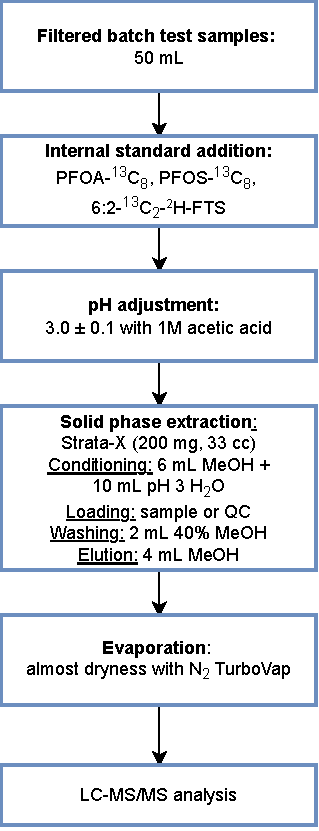
\includegraphics{Diagrams/Methods-Analytical_method.pdf}
    \caption{Schematic diagram of the analytical method applied for the determination target PFCs in the batch test filtrates adapted from \citep{arvaniti2012diagram}.}
    \label{fig:analyticalMethod}
\end{figure}

\subsection{SPE}
SPE is a sample preparation method used to concentrate a large-volume sample to an extract that can be submitted for analyte quantitation by LC-MS/MS. The sample is passed through a cartridge with a porous sorbent polymer that strongly retains polar compounds (\textpi-\textpi bonding, hydrogen bonding and hydrophobic interaction). The sorbed analytes are then eluted with an appropriate solvent, evaporated, and finally reconstituted to the desired extract volume. All samples are spiked with a mix of internal standards (ISs) to compensate for variations in extraction percentages and instrumental response by the MS/MS detector \citep{arvaniti2014}. To minimize risk of contamination during laboratory work, working benches were cleaned with acetone and covered with aluminum foil. Sterilized PP tubes were used during all steps of the protocol.

Strata-X\textsuperscript{\textregistered} 200 mg/6mL cartridges supplied by Phenomenex were used for SPE of the TCs in the filtered water samples. The sorbent polymer was a surface modified styrene divinylbenzene (\cref{fig:StatPhase}) with 33 \textmu m average particle diameter and surface area of 800 m\textsuperscript{2} g\textsuperscript{-1}. The internal standards used were \textsuperscript{13}C\textsubscript{8}-perfluorooctanoic acid  (\textsuperscript{13}C\textsubscript{8}-PFOA), \textsuperscript{13}C\textsubscript{8}-potassium perfluorooctanesulfonate (\textsuperscript{13}C\textsubscript{8}-PFOS-K), and 6:2-\textsuperscript{13}C\textsubscript{2}-\textsuperscript{1}H,\textsuperscript{2}H-perfluorooctane sulfonate  (6:2 \textsuperscript{13}C\textsubscript{2}-FTS) where a working standard of the three isotopic PFAS was prepared in methanol at 1 ppm from 50 ppm analytical standard supplied by Sigma Aldrich.

The samples were adjusted to pH $\sim$3 with 800 \textmu L 1 M acetic acid. However, the samples containing soil needed addition of at least double the amount to reach the same pH. pH was tested for five randomly selected samples for each batch of 20 was with pH strips. All samples were then spiked with IS. SC1 and SC2 samples were spiked with 10 \textmu L IS and SC3-SC10 samples were spiked with 20 \textmu L IS--the difference in amount of IS for the two low-spike samples being due to a more concentrated extract needed for these samples to avoid signals below instrumental LOQ. Therefore, SC1 and SC2 samples were made to 0.5 mL extracts instead of 1 mL as for the rest. The samples were vortexed prior to SPE.

The cartridges were placed in individual slots with LC liners on a TLC chamber and conditioned with 6 mL MeOH and 10 mL pH 3 milli-Q water (acidified by 100\% acetic acid). MeOH was used for wetting to allow the mobile phase into the pores of the sorbent polymer in order to ensure maximum chromatographic retention. Low-pH water was used to protonate loan electrons on the polymer surface so that hydrophobic interaction with the analytes were maximized. The samples were loaded using glass pipettes and allowed to pass through the cartridges with gravity. The flow rate was adjusted by modifying the opening of the LC liners so that the sample exited the cartridge as individual droplets. 

After loading the samples, the cartridges were washed with 2 mL MeOH:MQ (40:60, \% v/v) in order to remove any matrix interferences. The cartridges were then dried with a vacuum pump at 20 mmHg until the sorbent mass was visible as dry powder. The analytes were eluted with 4 mL MeOH into 15 mL PP centrifuge tubes, and concentrated to almost dryness ($\le$0.5 mL) using TurboVap\textsuperscript{\textregistered} at 40 \textdegree C and nitrogen gas (N\textsubscript{2}) at 5 psi. The samples were reconstituted to 1 mL (0.5 mL for SCs 1 and 2) with MeOH and milli Q to a final solvent ratio of 50:50 \% v/v. The extracts were transferred to LC vials using glass pipettes and stored at -19 \textdegree C until analysis.

\begin{figure}
    \centering
    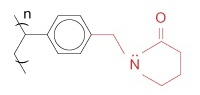
\includegraphics{Bilder/SPE_LCMS/mg_spe_strata-x.jpg}
    \caption{Sorbent polymer used for SPE, surface-modified styrene divinylbenzene.}
    \label{fig:StatPhase}
\end{figure}

\subsection{LC-MS/MS}
Liquid chromatography separates compounds in a mixture based on polarity by using a stationary phase that retards hydrophobic compounds while allowing more polar compounds to pass through faster along with the polar mobile phase. The compounds are then ionized by a strong voltage into fragment ions that are detected by a mass spectrometer that determines the mass of the transitions. Quantification of PFAS was determined by UPLC-MS/MS with an Acquity UPLC I-Class system connected to a Xevo TQ-S triple quadrupole mass spectrometer equipped with an ESI Z spray, both supplied by Waters (Milford, MA, USA). A Kinetex C18 column (30 x 2.1 mm, 1.3 \textmu m) serially connected to a Phenomenex C18 (2 x 2.1 mm i.d.) security guard (Torrance, CA, USA) was used for chromatographic separation. Mobile phases were A: 2 mM ammonium acetate in Milli-Q water (water phase) and B: pure MeOH (organic phase) that were supplied at a constant flow rate of 250 \textmu L min\textsuperscript{-1} to the LC column maintained at a temperature of 30 \textdegree C. The sample injection volume was 4 \textmu L. The run time for each sample was 6 minutes with an initial and final mobile phase gradient of 20:80 (A:B). Analytes were ionized by negative electrospray ionization (ESI-) and nitrogen was used as drying gas at the ionization source. Two ion transitions were monitored for each PFCA (\cref{tab:transitions}) within 60 s of the expected retention time for the compound. Peak integration was performed automatically by MassLynx software obtaining 12 points per peak and an average baseline peak width of 5 s. Data from UPLC-MS/MS was processed in MassLynx version 4.1 and quantification processing was performed with TargetLynx. Each peak was manually reviewed to remove peaks that were likely background noise as well as corrections for inconsistencies in peak base width. Complete instrument programming and parameters are summarized in \cref{appSec:LCMS}.

\begin{table}[tbh]
\centering
\caption{Ion transitions for the target analytes and internal standards in this study.}
\adjustbox{max width=\textwidth}{%
\begin{threeparttable}
\label{tab:transitions}
\begin{tabular}{ccccccl} \toprule
Compound &  Structure & Formula & M & Parent & Cone (V) & Transitions (CE)  \\ \midrule
& & & & & & \\
\multirow{2}{*}{PFPeA} &  \multirow{2}{*}{\chemfig[atom style={scale=0.5}]{O=[:90](-[:30,,,1]OH)-[:150](-[:112.5]F)(-[:67.5]F)-[:210](-[:292.5]F)(-[:247.5]F)-[:150](-[:112.5]F)(-[:67.5]F)-[:210](-[:270]F)(-[:150]F)-[:210]F}} & \multirow{2}{*}{$\mathrm{C_5HF_9O_2}$} & \multirow{2}{*}{264.05} & \multirow{2}{*}{262.97} & \multirow{2}{*}{20} & \multirow{2}{*}{262.97 $\rightarrow$ 219 (8)} \\
& & & & & & \\
& & & & & & \\
 &  &  &  &  &  &    \\
\multirow{2}{*}{PFHxA} &  \multirow{2}{*}{\chemfig[atom style={scale=0.5}]{O=[:90](-[:30,,,1]OH)-[:150](-[:112.5]F)(-[:67.5]F)-[:210](-[:292.5]F)(-[:247.5]F)-[:150](-[:112.5]F)(-[:67.5]F)-[:210](-[:292.5]F)(-[:247.5]F)-[:150](-[:210]F)(-[:150]F)-[:90]F}} & \multirow{2}{*}{$\mathrm{C_6HF_{11}O_2}$} & \multirow{2}{*}{314.05} & \multirow{2}{*}{312.97} & \multirow{2}{*}{10} & 312.97 $\rightarrow$ 118.95 (18) \\
 &  &  &  &  &  &   312.97 $\rightarrow$ 269 (8) \\
 & & & & & & \\
 & & & & & & \\
\multirow{2}{*}{PFHpA} &  \multirow{2}{*}{\chemfig[atom style={scale=0.5}]{O=[:90](-[:30,,,1]OH)-[:150](-[:67.5]F)(-[:112.5]F)-[:210](-[:247.5]F)(-[:292.5]F)-[:150](-[:67.5]F)(-[:112.5]F)-[:210](-[:247.5]F)(-[:292.5]F)-[:150](-[:67.5]F)(-[:112.5]F)-[:210](-[:150]F)(-[:210]F)-[:270]F}} & \multirow{2}{*}{$\mathrm{C_7HF_{13}O_2}$} & \multirow{2}{*}{364} & \multirow{2}{*}{362.96} & \multirow{2}{*}{6} & 362.96 $\rightarrow$ 119.00 (22) \\
 &  &  &  &  &  &   362.96 $\rightarrow$ 168.97 (18) \\
 & & & & & & \\
 & & & & & & \\
\multirow{2}{*}{PFOA} &  \multirow{2}{*}{\chemfig[atom style={scale=0.5}]{O=[:90](-[:30,,,1]OH)-[:150](-[:67.5]F)(-[:112.5]F)-[:210](-[:247.5]F)(-[:292.5]F)-[:150](-[:67.5]F)(-[:112.5]F)-[:210](-[:247.5]F)(-[:292.5]F)-[:150](-[:67.5]F)(-[:112.5]F)-[:210](-[:247.5]F)(-[:292.5]F)-[:150](-[:90]F)(-[:150]F)-[:210]F}} & \multirow{2}{*}{$\mathrm{C_8HF_{15}O_2}$} & \multirow{2}{*}{414.07} & \multirow{2}{*}{412.97} & \multirow{2}{*}{20} & 412.97 $\rightarrow$ 168.90 (18) \\
 &  &  &  &  &    & 412.97 $\rightarrow$ 369.00 (8) \\
 & & & & & & \\
 & & & & & & \\
\multirow{2}{*}{PFNA} &  \multirow{2}{*}{\chemfig[atom style={scale=0.5}]{O=[:90](-[:30,,,1]OH)-[:150](-[:112.5]F)(-[:67.5]F)-[:210](-[:292.5]F)(-[:247.5]F)-[:150](-[:112.5]F)(-[:67.5]F)-[:210](-[:292.5])(-[:247.5]F)-[:150](-[:112.5]F)(-[:67.5]F)-[:210](-[:292.5]F)(-[:247.5]F)-[:150](-[:112.5]F)(-[:67.5]F)-[:210](-[:270]F)(-[:210]F)-[:150]F}} & \multirow{2}{*}{$\mathrm{C_9HF_{17}O_2}$} & \multirow{2}{*}{464.08} & \multirow{2}{*}{462.99} & \multirow{2}{*}{20} & 462.99 $\rightarrow$ 219 (16) \\
 &  &  &  &  &    & 462.99 $\rightarrow$ 419 (10) \\
  & & & & & & \\
  & & & & & & \\
\multirow{2}{*}{PFDA} &  \multirow{2}{*}{\chemfig[atom style={scale=0.5}]{O=[:90](-[:30,,,1]OH)-[:150](-[:112.5]F)(-[:67.5]F)-[:210](-[:292.5]F)(-[:247.5]F)-[:150](-[:112.5]F)(-[:67.5]F)-[:210](-[:292.5]F)(-[:247.5]F)-[:150](-[:112.5]F)(-[:67.5]F)-[:210](-[:292.5]F)(-[:247.5]F)-[:150](-[:112.5]F)(-[:67.5]F)-[:210](-[:292.5]F)(-[:247.5]F)-[:150](-[:210]F)(-[:150]F)-[:90]F}} & \multirow{2}{*}{$\mathrm{C_{10}HF_{19}O_2}$} & \multirow{2}{*}{514.09} & \multirow{2}{*}{513.1} & \multirow{2}{*}{10} & 513.10 $\rightarrow$ 219.01 (18) \\
 &  &  &  &  &    & 513.10 $\rightarrow$ 269.04 (16) \\ 
 & & & & & & \\
 & & & & & & \\ \midrule
 \multicolumn{7}{c}{\textit{Internal standards (IS)}} \\ \midrule
  & & & & & & \\
 \multirow{2}{*}{PFOA \textsuperscript{13}C\textsubscript{8}} & \multirow{2}{*}{\chemfig[atom style={scale=0.5}]{O=[:90](-[:30,,,1]OH)-[:150](-[:67.5]F)(-[:112.5]F)-[:210](-[:247.5]F)(-[:292.5]F)-[:150](-[:67.5]F)(-[:112.5]F)-[:210](-[:247.5]F)(-[:292.5]F)-[:150](-[:67.5]F)(-[:112.5]F)-[:210](-[:247.5]F)(-[:292.5]F)-[:150](-[:90]F)(-[:150]F)-[:210]F}} & \multirow{2}{*}{$\mathrm{^{13}C_8HF_{15}O_2}$} & \multirow{2}{*}{422.01} & \multirow{2}{*}{420.9} & \multirow{2}{*}{16} & 420.90 $\rightarrow$ 171.86 (16) \\
 &  &  &  &  &    & 420.90 $\rightarrow$ 222.84 (16) \\ 
 & & & & & & \\
 & & & & & & \\
  \multirow{2}{*}{PFOS \textsuperscript{13}C\textsubscript{8}} & \multirow{2}{*}{\chemfig[atom style={scale=0.5}]{F-[:67.5](-[:292.5]F)(-[:30]S(=[:300]O)(-[:30,,,1]OH)=[:120]O)-[:150](-[:67.5]F)(-[:112.5]F)-[:210](-[:247.5]F)(-[:292.5]F)-[:150](-[:67.5]F)(-[:112.5]F)-[:210](-[:247.5]F)(-[:292.5]F)-[:150](-[:67.5]F)(-[:112.5]F)-[:210](-[:247.5]F)(-[:292.5]F)-[:150](-[:90]F)(-[:150]F)-[:210]F}} & \multirow{2}{*}{$\mathrm{^{13}C_8HF_{17}O_3}S$} & \multirow{2}{*}{507.06} & \multirow{2}{*}{506.9} & \multirow{2}{*}{56} & 506.90 $\rightarrow$ 79.87 (46) \\
 &  &  &  &  &    & 506.90 $\rightarrow$ 171.85 (32) \\ 
 & & & & & & \\
 & & & & & & \\ 
 \multirow{2}{*}{6:2 FTS \textsuperscript{13}C\textsubscript{2}} & \multirow{2}{*}{\chemfig[atom style={scale=0.5}]{O=[:60]S(=[:60]O)(-[:330,,,1]OH)-[:150]-[:210]-[:150](-[:67.5]F)(-[:112.5]F)-[:210](-[:247.5]F)(-[:292.5]F)-[:150](-[:67.5]F)(-[:112.5]F)-[:210](-[:247.5]F)(-[:292.5]F)-[:150](-[:67.5]F)(-[:112.5]F)-[:210](-[:270]F)(-[:210]F)-[:150]F}} & \multirow{2}{*}{$\mathrm{C_{6}^{13}C_2H_{5}F_{13}O_3S}$} & \multirow{2}{*}{432} & \multirow{2}{*}{432.96} & \multirow{2}{*}{26} & 432.96 $\rightarrow$ 411.959 (24) \\
 &  &  &  &  &    & 432.96 $\rightarrow$ 81.901 (30) \\ 
 & & & & & & \\
 & & & & & & \\ \bottomrule
\end{tabular}
\begin{tablenotes}
\item CE = collision energy
\item V = cone voltage
\end{tablenotes}
\end{threeparttable}}
\end{table}

\subsection{Quality assurance and quality control}
Accurate mass spectrometric quantitation was performed using the matrix-matched calibration method. Details about the quality control samples are in \cref{tab:QC}.

\subsubsection{Calibration curves}
A 10-point calibration curve ranging from 0.01 to 50 ppb was prepared in methanol. The results demonstrated a satisfactory regression coefficient ($r^2 > 0.98$) for each analyte. This solvent blank calibration curve is used to derive analyte concentrations in samples not taken through the SPE protocol since they do not experience a matrix effect. A matrix matched calibration curve was used for MS quantitation of the samples brought through SPE. 

During calculations of results, only \textsuperscript{13}C\textsubscript{8}-PFOA was used because it had the most similar retention time as the target analytes. 

\begin{table}[htb]
\caption{Quality assurance and quality controls.}
\centering
\adjustbox{max width=\textwidth}{%
\begin{threeparttable}
\label{apptab:QC}
\begin{tabular}{lcccccc}
\toprule
\multicolumn{1}{c}{Code} & \begin{tabular}[c]{@{}c@{}} Sample \\ matrix\end{tabular} & \begin{tabular}[c]{@{}c@{}}TA (addition \\ pre-extraction)\end{tabular} & \begin{tabular}[c]{@{}c@{}}IS (addition \\ pre-extraction)\end{tabular} & \begin{tabular}[c]{@{}c@{}}TA (addition \\ post-extraction)\end{tabular} & \begin{tabular}[c]{@{}c@{}}IS (addition\\  post-extraction\end{tabular} & \multicolumn{1}{c}{\begin{tabular}[c]{@{}c@{}}Solvent\\ (MQ:MeOH)\end{tabular}} \\ \midrule
Procedural blank & NO &  & \checkmark &  & & 50:50 \\ \hline
Blank 1 & YES &  & \checkmark &  & & 50:50 \\ 
Blank 2 & YES &  & \checkmark &  & & 50:50 \\ \hline
Spike 2.5 ppb & YES & \checkmark & \checkmark &  & & 50:50 \\ 
Spike 25 ppb & YES & \checkmark & \checkmark &  & & 50:50 \\ 
Spike 50 ppb & YES & \checkmark & \checkmark &  &  & 50:50\\ \hline
Matrix matched 2.5 ppb & YES &  &  & \checkmark & \checkmark & 50:50\\
Matrix matched 25 ppb & YES &  &  & \checkmark & \checkmark & 50:50\\
Matrix matched 50 ppb & YES &  &  & \checkmark & \checkmark & 50:50\\ \hline
Solvent blank\tnote{*} & NO & & & & & 0:100\\
Calibration 0 ppb & NO &  &  & \checkmark & \checkmark & 0:100 \\ 
Calibration 0.01 ppb & NO&  &  & \checkmark & \checkmark & 0:100\\
Calibration 0.05 ppb & NO&  &  & \checkmark & \checkmark & 0:100\\
Calibration 0.1 ppb & NO&  &  & \checkmark & \checkmark & 0:100\\
Calibration 0.2 ppb & NO&  &  & \checkmark & \checkmark & 0:100\\
Calibration 0.5 ppb & NO&  &  & \checkmark & \checkmark & 0:100\\
Calibration 1 ppb & NO&  &  & \checkmark & \checkmark & 0:100\\
Calibration 2 ppb & NO&  &  & \checkmark & \checkmark & 0:100\\
Calibration 5 ppb & NO&  &  & \checkmark & \checkmark & 0:100\\
Calibration 10 ppb\tnote{*} & NO &  &  & \checkmark & \checkmark & 0:100\\
Calibration 25 ppb & NO&  &  & \checkmark & \checkmark & 0:100\\
Calibration 50 ppb & NO&  &  & \checkmark & \checkmark & 0:100\\ \bottomrule
\end{tabular}
\begin{tablenotes}
\item[*] Injected every 15-20 samples
\item TA = target analytes, IS = internal standard
\end{tablenotes}
\end{threeparttable}}
\end{table} %table with quality control parameters

\subsubsection{Blanks}
Contamination that may arise during preparation of samples and from laboratory materials was evaluated through the analysis of sample and procedural blanks. One procedural blank was prepared by spiking IS directly into the cartridge and eluting with methanol, continuing SPE from this point. Contamination from test tubes, reagents or other introductions of contamination will show up on the instrument results from this QA. Two blank samples were prepared by bringing 50 mL pH 3 MQ water (sample matrix) spiked with IS through the extraction protocol. Sample blanks determine any interferences caused by the the matrix itself. During analysis, solvent blanks (100 \% MeOH) and a standard mixture of TAs at 10 ppb were injected every 15-20 samples to monitor potential cross contamination, carryover, and assuring maintenance of sensitivity. A MeOH:Milli-Q (50:50; v/v) 0.1 \% formic acid wash solution was used to clean the injection needle before and after each injection.

\subsubsection{Pre- and post- extraction spiked matrix samples}
QA/QC pre- and post-extraction matrix spike samples were prepared in triplicates at a concentration interval covering the expected concentration range of the test samples (2.5, 25 and 50 ppb). A working standard of target analytes (C5-C10) was prepared at 1 ppm in MeOH for spiking the samples. Pre-extraction matrix spikes were prepared by spiking IS and TA standard at 2.5, 25 and 50 ppb in 50 mL sample matrix. These were taken through the protocol in the same manner as the test samples. Matrix matched samples were prepared by taking 50 mL sample matrix through the SPE protocol and spiking with 2.5, 25 and 50 ppb TA and IS post-extraction. Concentration of TAs was determined with the resulting matrix matched calibration curve. 

\subsubsection{Absolute recovery, relative recovery and matrix effect calculations}
Recovery (R), relative recovery (RR) and matrix effects (ME) were calculated for each TA by comparing the pre- and post-extraction matrix spike signals. R and RR were assessed by the the following equations:

\begin{equation}
    \label{eq:Recovery}
    \mathrm{\% AR  = 100 \% \times \left ( \frac{A_{ss}}{A_{se}} \right ) }
\end{equation}

\begin{equation}
    \label{eq:relativeRecovery}
    \mathrm{\% RR = \frac{\frac{A_{ss}}{A_{is}}-\frac{A_{b}}{A_{is}}}{\frac{A_{se}}{A_{is}}-\frac{A_{b}}{A_{is}}}\times 100 \% }
\end{equation}

where 100 \% indicates recovery of all analytes. Matrix effects is assessed by the following equation:

\begin{equation}
    \label{eq:ME}
    \mathrm{\% ME = 100 \% \times \left(\frac{A_{se} - A_b}{A_{cc}}\right )-1 }
\end{equation}

where ME \textgreater 0\% indicates ion enhancement, and ME \textless 0\% = ion suppression. Matrix effects (MEs, \%) during measurements were assessed and estimated as X, X, X, X, X, X for PFPeA, PFHxA, PFHpA, PFOA, PFNA, and PFDA, respectively.

Where: \newline
\newline
\begin{tabular}{p{1cm}p{20cm}}
    \textit{A}   & peak area of chromatogram signal, \\
    \textit{ss}  & spiked sample (pre-extraction matrix spike), \\
    \textit{se}  & spiked extract (post-extraction matrix matched), \\
    \textit{is}  & internal standard, \\
    \textit{b}   & solvent blank, \\
    \textit{cc}  & calibration curve solvent spike \\
\end{tabular} \\

%%%%%%%%%%%%%%%%%%%%%%%%%%%%%%%%%%%%%%%%%%%%%%%%%%%%%%%%%%%%%%%%%%%%%%%%%%%%%%%%%%%%%%%%%%%%%%%%%%%%%%%%%%%%%%%%%%%%%%%%%%%

\section{Data analysis}
Chromatogram analysis and peak integration for PFAS quantification were carried out using MassLynx version and TargetLynx versions 4.1.  Raw data handling was conduced using Microsoft Excel (v.16.58). Statistical analysis and plotting were carried out using R software (v.4.1.2) and RStudio IDE (2022.02.0-443).

\newpage

%Lab analysis

\newpage

\part{Results and discussion}
\chapter{Results and discussion}\label{chap:Results&Disc}
In this chapter the results and methods from laboratory experiments are presented and discussed.

\section{PFCA sorption behavior}
\subsection{Biochar-water sorption isotherms}
In \cref{fig:sorption_isotherms}, the sorption isotherms are presented for PFPeA, PFHxA, PFHpA, PFOA, PFNA and PFDA to CWC, ULS and DSL. The points generated from the batch tests were fitted using the Freundlich model (\cref{eq:FreundlichLinear}). For all compounds, the sorption isotherm for ULS is visibly higher than DSL, followed by CWC. The Freundlich sorption coefficients ($log~K_F$), linearity coefficients ($n_F$) and correlation coefficients ($r^2$) are presented in \cref{tab:summary_stats_single}. Somewhat unexpectedly, sorption is strongest for the two sludge chars. Possible mechanisms for the strong sorption will be discussed in this section. 

Due to the pioneering research on sewage sludge biochars as sorbents for PFAS in this thesis, literature partitioning coefficients for PFCAs of other sewage sludge biochars are non-existent (is that correct?). However, a comparison can be made between the $log~K_F$s found in this thesis and for commercially-produced activated carbons (AC) reported in other studies. The sorption coefficients are equivalent or higher compared to literature values for $log~K_F$ of PFOA to AC: 5.60 \citep{Kupryianchyk2016a}, 4.45 \citep{hansen2010sorption}, and 4.74-5.42 \citep{silvani2019can}. This is promising for the potential to replace non-renewable AC with waste based biochars for environmental remediation in the field and wastewater treatment. 

\begin{figure}[tb]
    \centering
    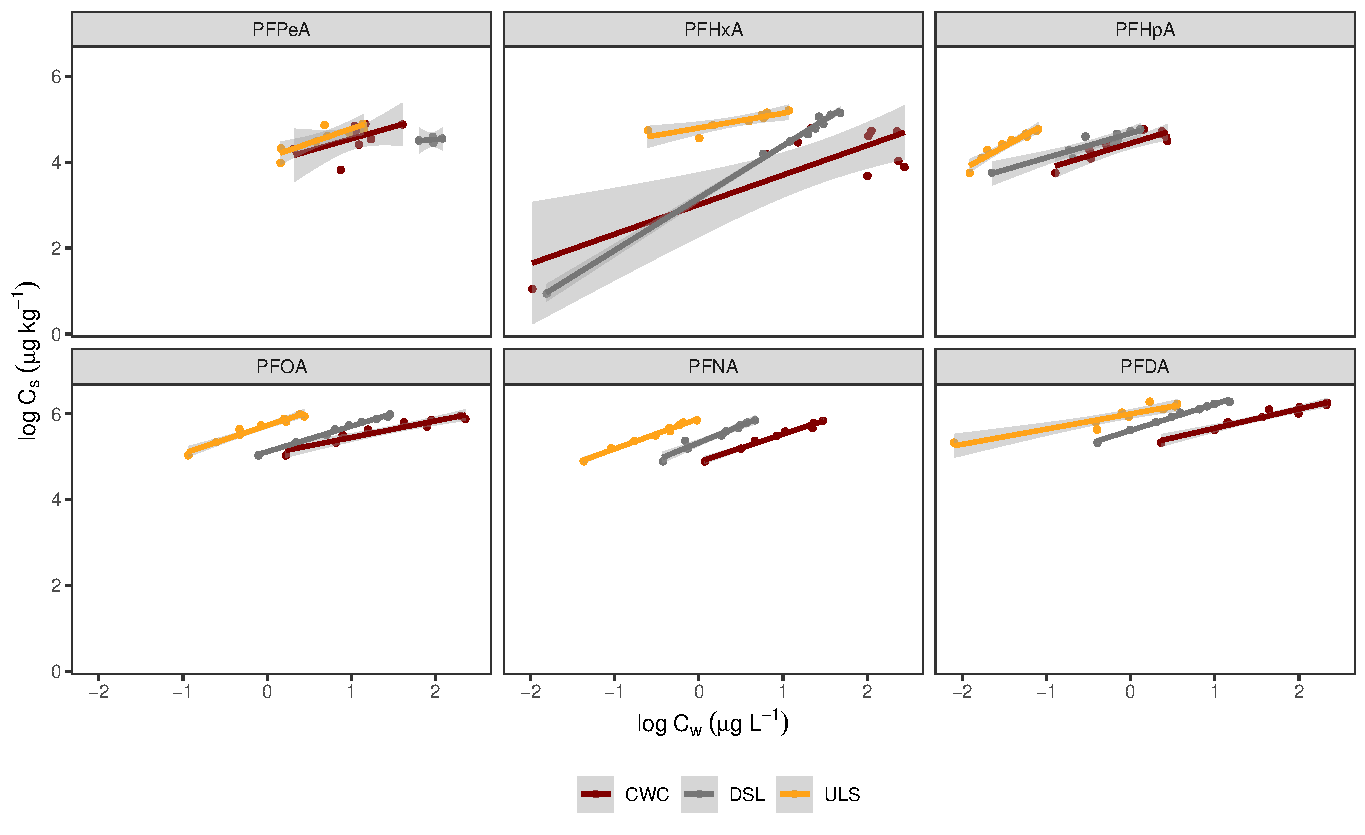
\includegraphics[width=0.8\textwidth]{R/figs/Sorption_isotherms_single_BC.pdf}
    \caption{Freundlich sorption isotherms of TCs in batch tests with three different biochars. Lines are obtained by linear regression.}
    \label{fig:sorption_isotherms}
\end{figure}

\begin{table}
\caption{Freundlich sorption parameters of single TC isotherms in CWC, ULS and DSL (n=9). The error is presented as standard error. All $K_F$ data are in units of $\mathrm{(\mu g/kg)/(\mu g/L)^{n_F}}$.}
\centering
\adjustbox{max width=\textwidth}{%
\begin{threeparttable}
\label{tab:summary_stats_single}
\begin{tabular}{lllllllllllll} \toprule
PFCA & \multicolumn{4}{c}{ULS} & \multicolumn{4}{c}{DSL} & \multicolumn{4}{c}{CWC} \\ \cmidrule(l){2-5} \cmidrule(l){6-9} \cmidrule(l){10-13}
 & $log~K_{F,BC}$ & $n_{F,BC}$ & $r^2$ & $p$ & $log~K_{F,BC}$ & $n_{F,BC}$ & $r^2$ & $p$ & $log~K_{F,BC}$ & $n_{F,BC}$ & $r^2$ & $p$ \\ \midrule
PFPeA & 4.10 ± 0.13 & 0.67 ± 0.16 & 0.74 & ** & 4.25 ± 0.74 & 0.14 ± 0.38 & 0.06 & $>$0.05 & 3.98 ± 0.36 & 0.56 ± 0.33 & 0.30 & $>$0.05 \\
PFHxA & 4.80 ± 0.06 & 0.34 ± 0.09 & 0.72 & ** & 3.30 ± 0.15 & 1.11 ± 0.11 & 0.93 & *** & 4.59 ± 0.50 & -0.14 ± 0.26 & 0.04 & $>$0.05 \\
PFHpA & 5.98 ± 0.17 & 1.08 ± 0.11 & 0.93 & *** & 4.67 ± 0.06 & 0.57 ± 0.09 & 0.86 & *** & 4.44 ± 0.05 & 0.59 ± 0.11 & 0.80 & ** \\
PFOA & 5.73 ± 0.02 & 0.65 ± 0.05 & 0.95 & *** & 5.12 ± 0.02 & 0.60 ± 0.02 & 0.99 & *** & 5.06 ± 0.08 & 0.39 ± 0.05 & 0.90 & *** \\
PFNA & 5.89 ± 0.02 & 0.71 ± 0.03 & 0.99 & *** & 5.33 ± 0.03 & 0.80 ± 0.07 & 0.94 & *** & 4.88 ± 0.04 & 0.65 ± 0.04 & 0.98 & *** \\
PFDA & 6.00 ± 0.04 & 0.35 ± 0.05 & 0.86 & *** & 5.61 ± 0.02 & 0.61 ± 0.02 & 0.99 & *** & 5.22 ± 0.07 & 0.45 ± 0.04 & 0.94 & *** \\ \bottomrule
\end{tabular}
\begin{tablenotes}
\item Significant codes: *** $\sim$ 0.001, ** $\sim$ 0.01  
\end{tablenotes}
\end{threeparttable}}
\end{table}

\subsection{Effect of PFCA properties}
\subsubsection{PFCA chain length}
\cref{fig:sorption_isotherms_all} shows sorption isotherms for the single-compound batch tests for CWC, ULS and DSL. The Freundlich coefficients for ULS increased in the order, PFPeA $<$ PFHxA $<$ PFOA $<$ PFHpA $<$ PFNA $<$ PFDA, ranging from $log~K_F$ = 4.10-6.00 (\cref{tab:summary_stats_single}). All regressions were significant (p$<$0.01). The Freundlich coefficients for DSL increased in the order, PFHxA $<$ PFPeA $<$ PFHpA $<$ PFOA $<$ PFNA $<$ PFDA, ranging from $log~K_F$ = 3.16-5.61. All regressions were significant (p$<$0.001) except for the PFPeA isotherm which only consisted of four points (SP7-10) due to higher analyzed filtrate concentrations than what was spiked for SP1-6 (attributed to analytical uncertainty or imprecision/contamination during laboratory work) (\cref{fig:DSL_isotherm}). The Freundlich coefficients for CWC increased in the order, PFPeA $<$ PFHpA $<$ PFHxA $<$ PFNA $<$ PFOA $<$ PFDA, ranging from $log~K_F$ = 3.01-5.22. All regressions were significant (p$<$0.01) except for PFPeA and PFHxA despite nine points used in the regressions. Changes in $log~K_F$ with chain length can be visualized in \cref{subfig:chainlength}. 

A statistically significant relationship between $log~K_F$ and CF\textsubscript{2} chain length was found for all three biochars (p$<$0.05, \cref{fig:chain_length_n}), which is in accordance with previous studies \citep{Sorengard2019,higgins2006sorption,ahmed2020per}. There was a difference of 1.2-1.9 $log~K_F$ units between the longest and the shortest PFCA chain (PFDA and PFPeA). For every CF\textsubscript{2} moiety, hydrophobic interactions between condensed aromatic structures in the biochar matrix increases, contributing to stronger sorption. Several mechanisms can be used to explain why perfluorinated carboxylic acids increase in hydrophobicity with increasing chain length. 1) Due to high molecular surface of the perfluorinated tail, a high cavity formation energy is needed to dissolve the compounds in water, and therefore they tend to be pushed towards water extremities, such as a biochar surface. Therefore, dissolution becomes increasingly energetically demanding with increasing chain length \citep{sigmund2022sorption}. 2) the perfluorinated chain with CF\textsubscript{2} moieties is capable of the least van der Waals interactions per molecular surface area compared to CH\textsubscript{2} which results in the least interactions between water molecules when in the water cavity. This is why PFASs are both oil- and water repellent. 

\begin{figure*}[tbh]
    \centering
    \begin{subfigure}[t]{0.45\textwidth}
        \centering
        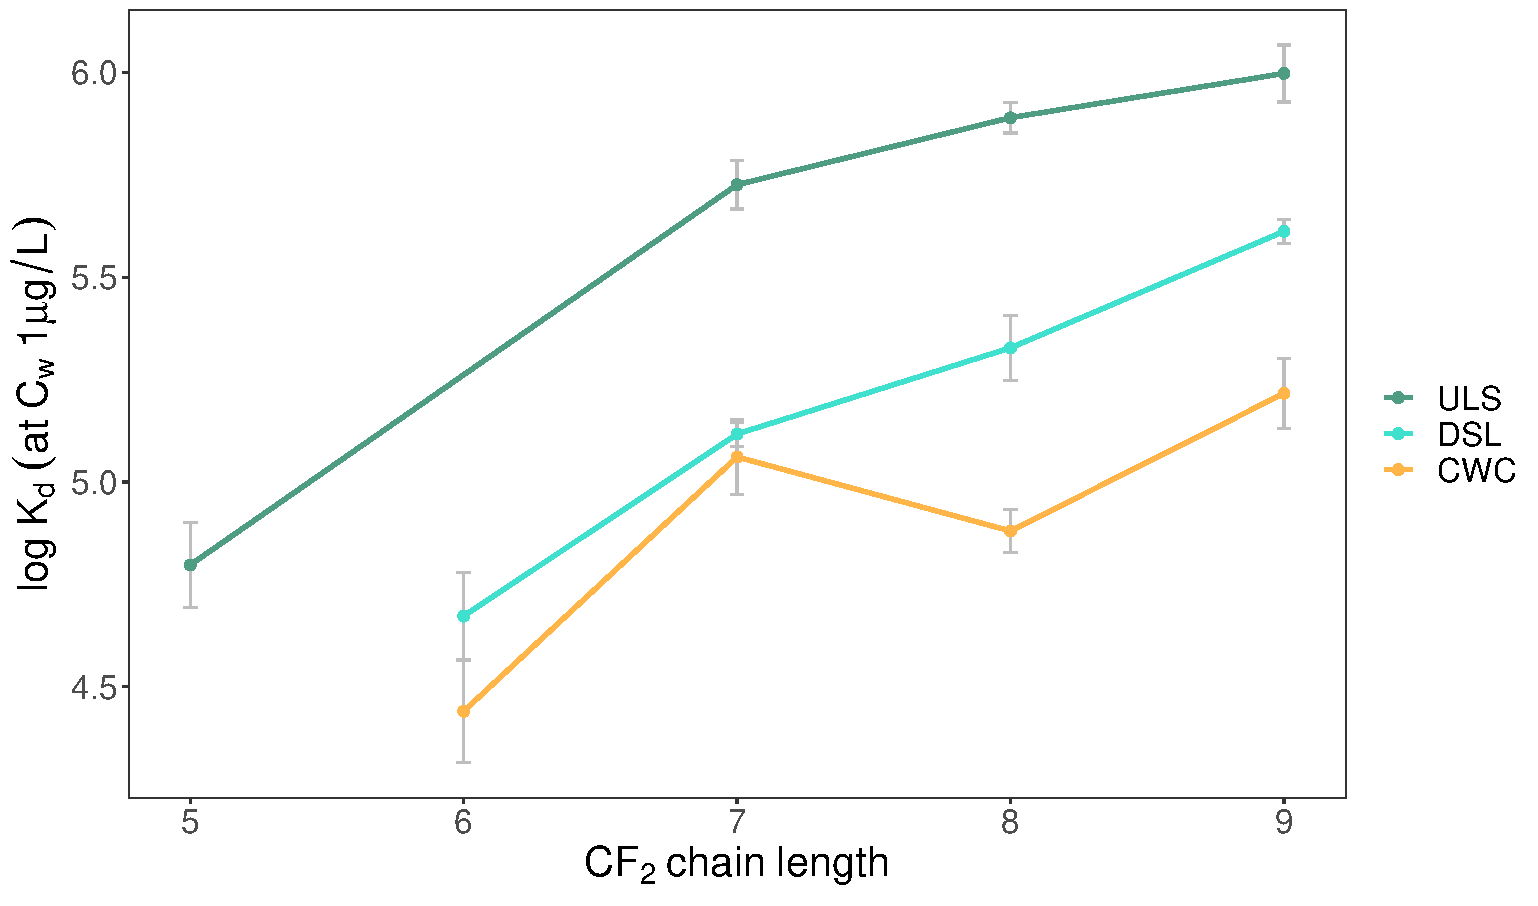
\includegraphics[width=\textwidth]{R/figs/chain_length_Kd1ugL_plot.pdf}
        \caption{}
        \label{subfig:chainlength}
    \end{subfigure}%
    ~ 
    \begin{subfigure}[t]{0.45\textwidth}
        \centering
        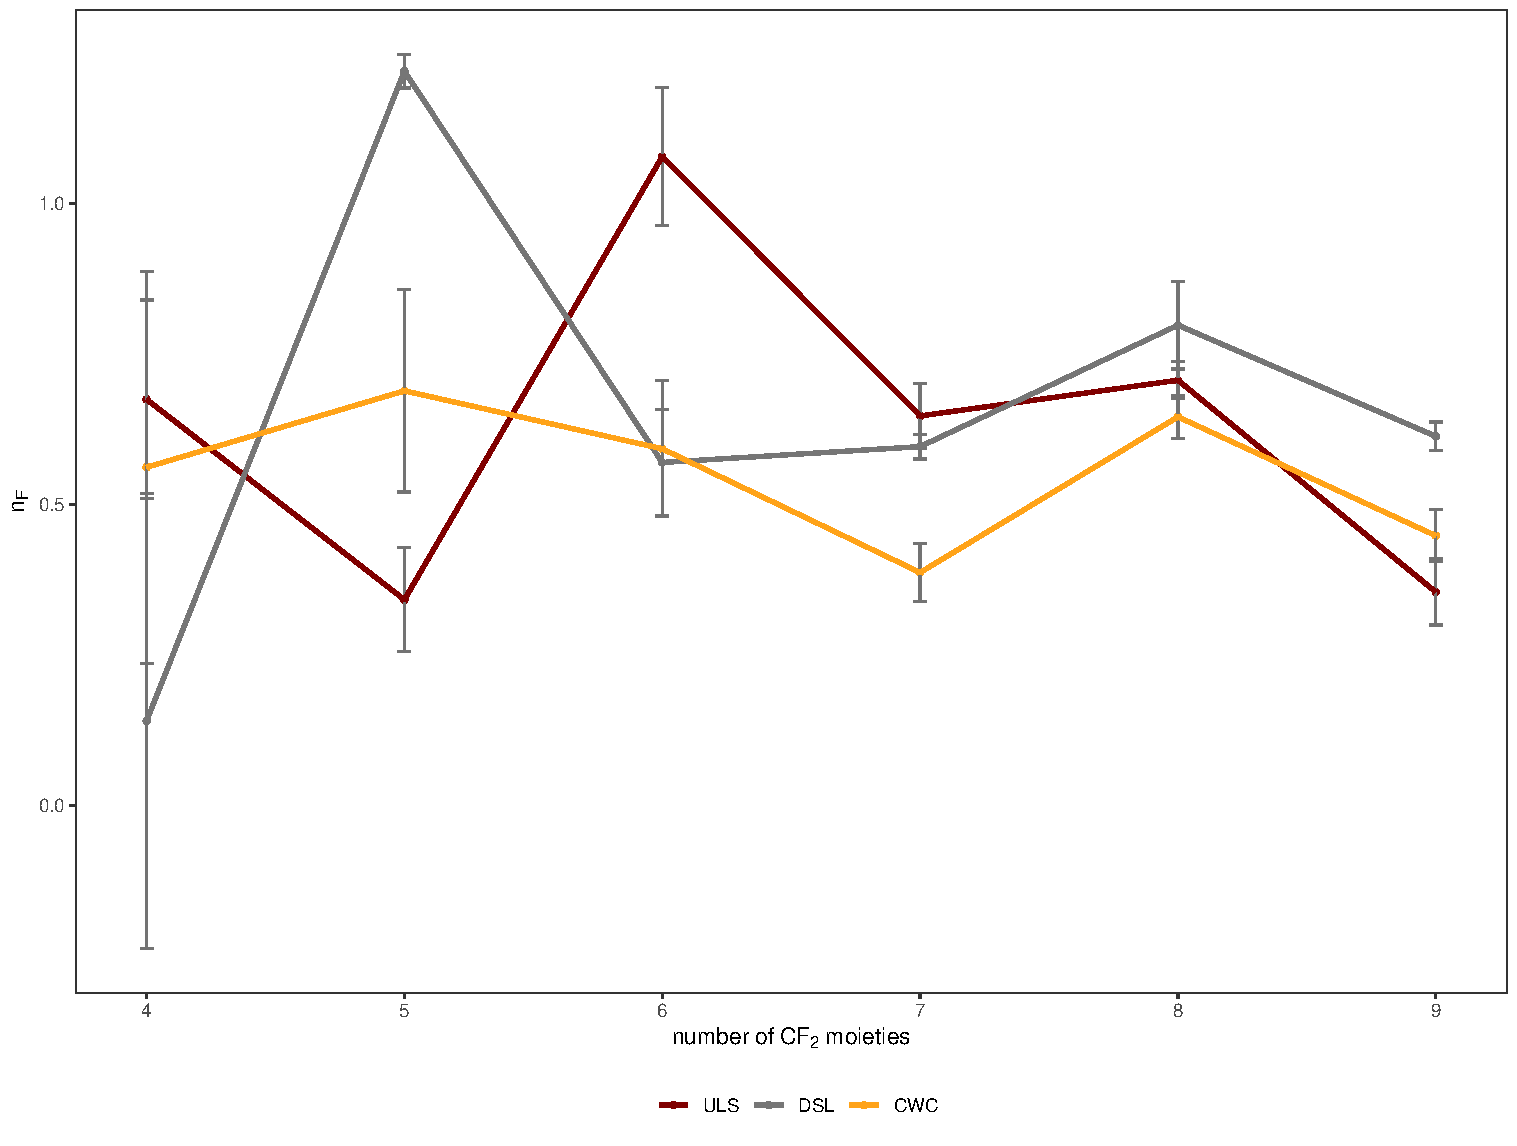
\includegraphics[width=\textwidth]{R/figs/n_KF.pdf}
        \caption{}
        \label{subfig:n}
    \end{subfigure}
    \label{fig:chain_length_n}
    \caption{Relationship between \textbf{(a)} Correlation between $log~K_F$ and chain length. Linear regression coefficients for ULS: $r^2$ = 0.68, $p$ = 0.52, DSL: $r^2$ = 0.98, $p$ = 0.012, CWC: $r^2$ = 0.93, $p$ = 0.007. Error bars are the propagated error of $log~K_F$ and $n_F$. \textbf{(b)} $n_F$ and $CF_2$ chain length. Error bars are the standard error of $log~K_F$ for each chain length and biochar isotherm.}
\end{figure*}

\begin{figure}
    \centering
        \begin{subfigure}[]{\linewidth}
            \centering
            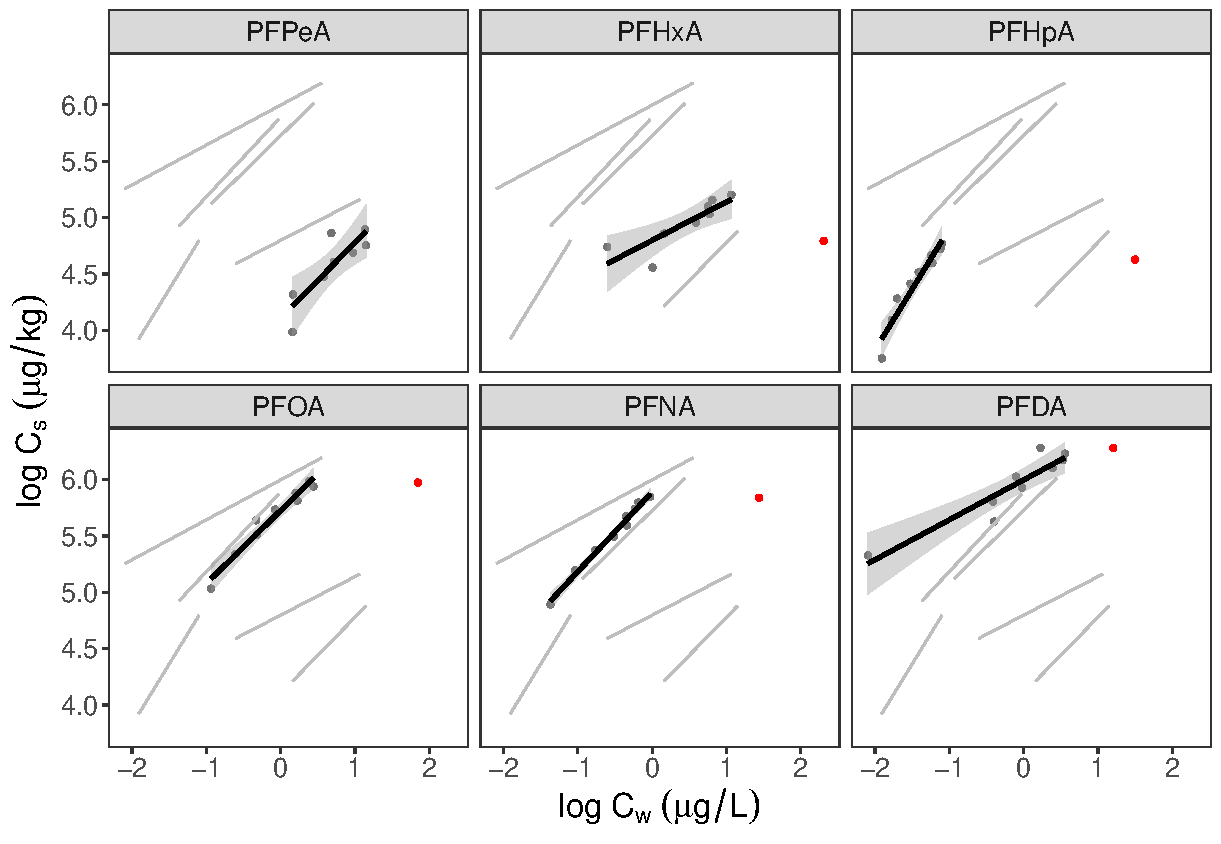
\includegraphics[width=0.6\textwidth]{R/figs/ULS_facet_isotherm.pdf}
            \subcaption{ULS isotherms}
            \label{fig:ULS_isotherm}
        \end{subfigure}
        \begin{subfigure}[]{\linewidth}
            \centering
            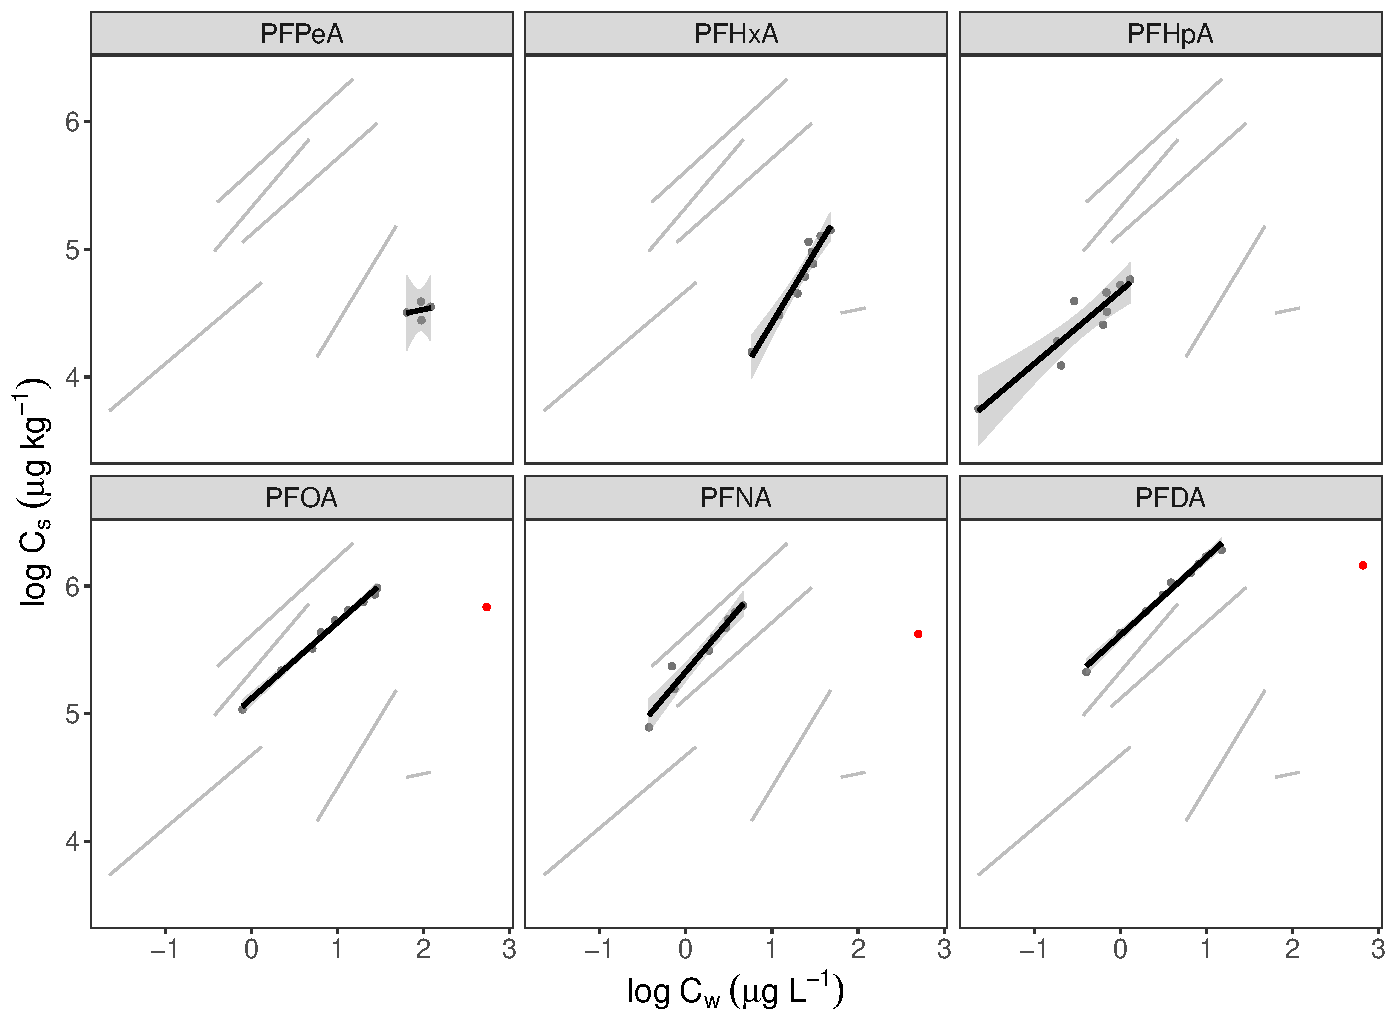
\includegraphics[width=0.6\textwidth]{R/figs/DSL_facet_isotherm.pdf}
            \subcaption{DSL isotherms}
            \label{fig:DSL_isotherm}
        \end{subfigure}   
\end{figure}
\begin{figure}[t]\ContinuedFloat
        \begin{subfigure}[]{\linewidth}
            \centering
            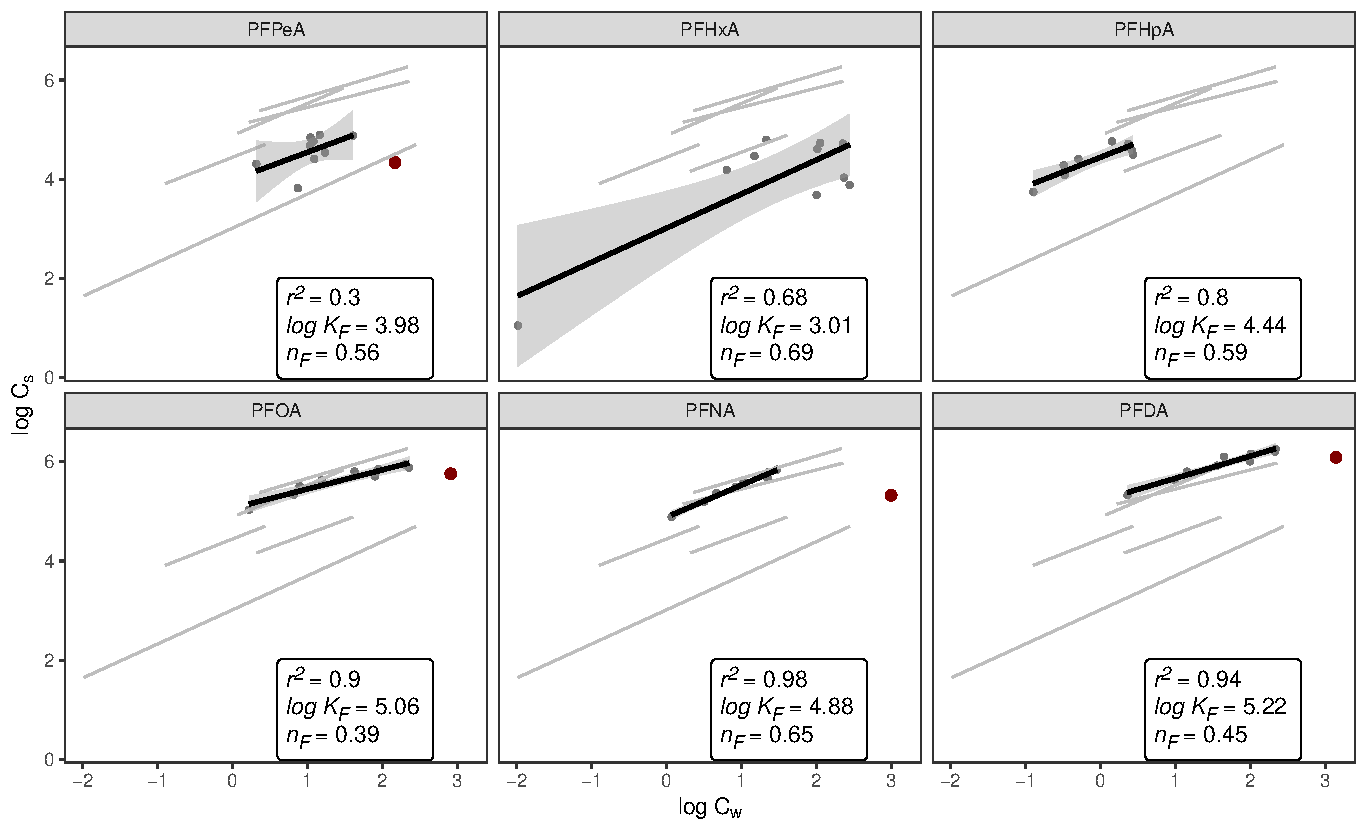
\includegraphics[width=0.6\textwidth]{R/figs/CWC_facet_isotherm.pdf}
            \subcaption{CWC isotherms}
            \label{fig:CWC_isotherm}
        \end{subfigure}
        \caption{Single-compound Freundlich sorption isotherms of PFPeA, PFHxA, PFHpA, PFOA, PFNA and PFDA. Lines are obtained by linear regression. For comparison across chain length, the shaded gray lines are the isotherms from the other compounds.}
        \label{fig:sorption_isotherms_all}
\end{figure}

\subsubsection{PFAS functional group} 
The charged and polar head of PFCAs give these compound classes unique sorptive properties because the polar head can engage simultaneously in electrostatic bonding with surface functional groups or bridging cations within the biochar matrix (ash rich in cations) \citep{zhang2013sorption,sigmund2022sorption}. In this study, the highest sorption were seen for ULS and DSL with the lowest \% C (\cref{tab:SAPV}), which is in contrast with previous literature. However, previous PFAS sorption studies have been conducted on biochar from cleaner, wood-based feedstock \citep{Sormo2021}, activated carbon \citep{zhang2021sorption,Kupryianchyk2016b}, soils and sediments \citep{higgins2006sorption}, and raw sewage sludges \citep{zhang2013sorption}. These studies conclude that the importance of electrostatic interaction to sorption comes secondary to the hydrophobic effect. The main reason for this is that the biochar surface is net negatively charged with a high cation exchange capacity (CEC) \citep{Ahmad2014} and may experience electrostatic repulsion of the negatively charged functional group on the PFAS (Include PZC when available). PFCAs have low $pK_a$s (-1, \citep{goss2008pKa}) due to having strong electron withdrawing fluorine atoms and hence become strong acids. The PFCAs investigated in this study will be negatively charged given the filtrate pH of 7.1-7.4 (\cref{tab:pHcond}). Thus, all TCs experience electrostatic repulsion from the biochar surface which result in the lowest $K_F$-values for the shorter-chain PFCAs (\cref{tab:summary_stats_single}). Electrostatic repulsion is reduced in acid soils where the CEC is reduced and the biochar surfaces become protonated and more neutral. This allows for anion- \textpi-bond interaction with biochar \citep{sigmund2022sorption}. 

\cite{zhang2021sorption} found that sorption increased in the order PFBA $<$ PFBS $<$ PFOA $<$ PFOS for granular activated carbon and softwood-derived biochar. The difference between the PFSA and PFCA groups is that PFSAs have one more perfluorinated carbon than PFCAs, which has its terminal carbon bonded as a carboxylate (COO\textsuperscript{-}). If one compares PFHpS with PFOA, which have the same number of $\mathrm{CF_2}$ moieties, the perfluorinated sulfonic acid still sorbs better. Researchers attribute this to 1) difference in molecular size, where the sulfonate moiety is slightly larger than the carboxylate moiety, which results in greater cavity formation energy of PFSAs, and hence in water saturated conditions, the functional group is pushed towards water extremities \citep{yin2022insights,sigmund2022sorption}. In batch shaking experiments this would be the biochar surfaces or tube walls; 2) Because sulfonic acid is a stronger acid than carboxylic acid which results in stronger ionic interaction to positive charges of mineral phases \citep{arvaniti2015review}. \cite{du2014adsorption}: electr and hydry balance Since sorption increased with chain length onto all three biochars in this study, this suggests that hydrophobic interactions is the dominant sorption mechanism over electrostatic interactions. Therefore, further investigation to explain why the sludge biochars sorb better than CWC will follow. 

%%%%%%%%%%%%%%%%%%%%%%%%%%%%%%%%%%%%%%%%%%%%%%%%%%%%%%%%%%%%%%%%%%%%%%%%%%%%%%%%%%%%%%%%%%%%%%%%%%%%%%%%%%%%%%%%%%%%%%%%%%%%%%%%%%%%%%%%%%%%%%%%%%%%%%%%%%%%%%%%%%%%%%%%%%%%%%%%%%%%%%%%%%%%%%%%%%%%%%%%%%%%%%%%%%%%%%%%%%%%%%%%%%%%%%%%%%%%%%%%%%%%%%%%%%%%%%%%%%%%%%%%%%%%%%%%%%%%%%%%%%%%%%%%%%%%%%%%%%%%%%%%%%%%%%%%%%%%%%%%%%%%%%%%%%%%%%%%%%%%%%%%%%%%%%%%%%%%%%%%%%%%%%%%%%%%%%%%%%%%%%%%%%%%%%%%%%%%%%%%%%%%%%%%%%%%%%%%%%%%%%%%%%%%%%%%%%%%%%%%%%%%%%%%%%%%%%%%%%%%%%%%%%%%%%%%%%%%%%%%%%%%%%%%%%%%%%%%%%%%%%%%%%%%%%%%%%%%%%%%%%%%%%%%%%%%%%%%%%%%%%%%

\section{Sorption attenuation by soil and competing congeners}
\cref{fig:C10} shows the $K_d$ values for the different batch test categories spiked at SC10 for each compound (\cref{tab:spikeConcentrations}, note: $K_d$-values cannot be compared between compounds as different spike concentrations were used). The figure shows that sorption is clearly attenuated by soil and competing congeners by varying degrees. Strongest sorption is seen and expected for the singly spiked batch tests with biochar only. The cocktail spikes in both biochar only and biochar and soil experience similar attenuation, although for ULS, BC soil cocktail is markedly lower than  BC cocktail, which is to be expected because the sandy soil used has poor sorption affinity with a mean $log~K_d$ value of 2.47 (red symbols, \cref{fig:C10}) versus $log~K_d$ of, for example, 6.06 for singly-spiked PFDA to ULS-water. Overall, BC soil cocktail experiences highest sorption attenuation, which is plausible because both soil and competing PFCAs disrupt optimal sorption. 

Single-spikes in soil was only performed for PFOA, whose sorption is weaker than BC single, but stronger than cocktails in both BC and BC-soil. This suggests that sorption attenuation by competing congeners is higher than by the presence of soil. Applied to real-world conditions, this means that soil amended with BC is more effective in removing PFCAs at low concentrations than highly contaminated soil with a mixture of compounds and highly concentrated PFCA-cocktail in water. 

A table of attenuation factors for each batch test category is provided in \cref{apptab:attenuation}.

\subsection{Attenuation by competing congeners}

\subsection{Attenuation by soil}
The soil used in the batch tests was characterized as a fine sand (0.1 to 0.3 mm) with 1.3 \% TOC (pH 5.38 \textpm 0.02, CEC 2.63 \textpm 0.06 meqv 100 g\textsuperscript{-1}). Total element concentrations and exchangeable ion concentrations are in \cref{appSec:elements}, \cref{apptab:soil}. 

Soil extraction showed no native target analytes present. Upon filtration, each batch test category was different in its ease of filtration due to various degree of suspended particles and had different color filtrate, as seen in \cref{subfig:filtrate}. Filter clogging and reduction in filter pore size, had to exchange filters during filtration, which is a potential source of error. 

Aggregation of humic substances upon addition of acetic acid pre-SPE, how this may impact results. 

Precipitation of a brown fluff was observed when filtered batch tests containing soil was adjusted to pH 3 with 1 M acetic acid

Sorptive attenuation of a spiked cocktail of the six TCs were tested for each biochar is shown by the red point in \cref{fig:sorption_isotherms_all}. Due to different spike concentration used for each compound in the cocktail, establishing quantitative trends for how chain length influences competition for sorption size is difficult. However, some conclusions can be drawn by looking at the overall trends. \cref{tab:competition} shows that $log~K_d$ decreases for all compounds in the presence of a mixture. $K_d$ changes the least for PFHxA and PFHpA (2.3 and 0.2 \% respectively) and may be attributed to lower spiked concentrations (330 and 117 \textmu g L\textsuperscript{-1}) for these compounds compared to the rest in \cref{tab:competition}. Competition is most profound for PFOA to CWC followed by PFDA for ULS and CWC (15.8, 10.0 and 10.6 \% respectively), which can be explained by the highest concentrations spiked for these compounds (1 953 and 3 830 \textmu g L\textsuperscript{-1}). It appears that sorption of PFNA is minimally influenced by competition between other compounds despite SC being in the higher range (1 409 \textmu g L\textsuperscript{-1}). $K_d$ for PFPeA is reduced by 8.2\% and is expected based on weaker sorption of short-chain compounds.

Expected: Attenuation factors larger for short-chain than long chains which have greater sorption affinity.

Most previous studies have reported a linear increasing trend between $log~K_d$ and chain length. However not for PFPeA, \citep{zhang2013sorption}, found in \citep{Sorengard2019}. and \citep{guelfo2013} these studies are for sorption to organic matter.  Steric hindrance. Competing sorption to humic matter
fouling/pre-loading by NOM
Pore blocking

\begin{figure}[htb]
\subfloat[\label{subfig:filtrate}]{%
  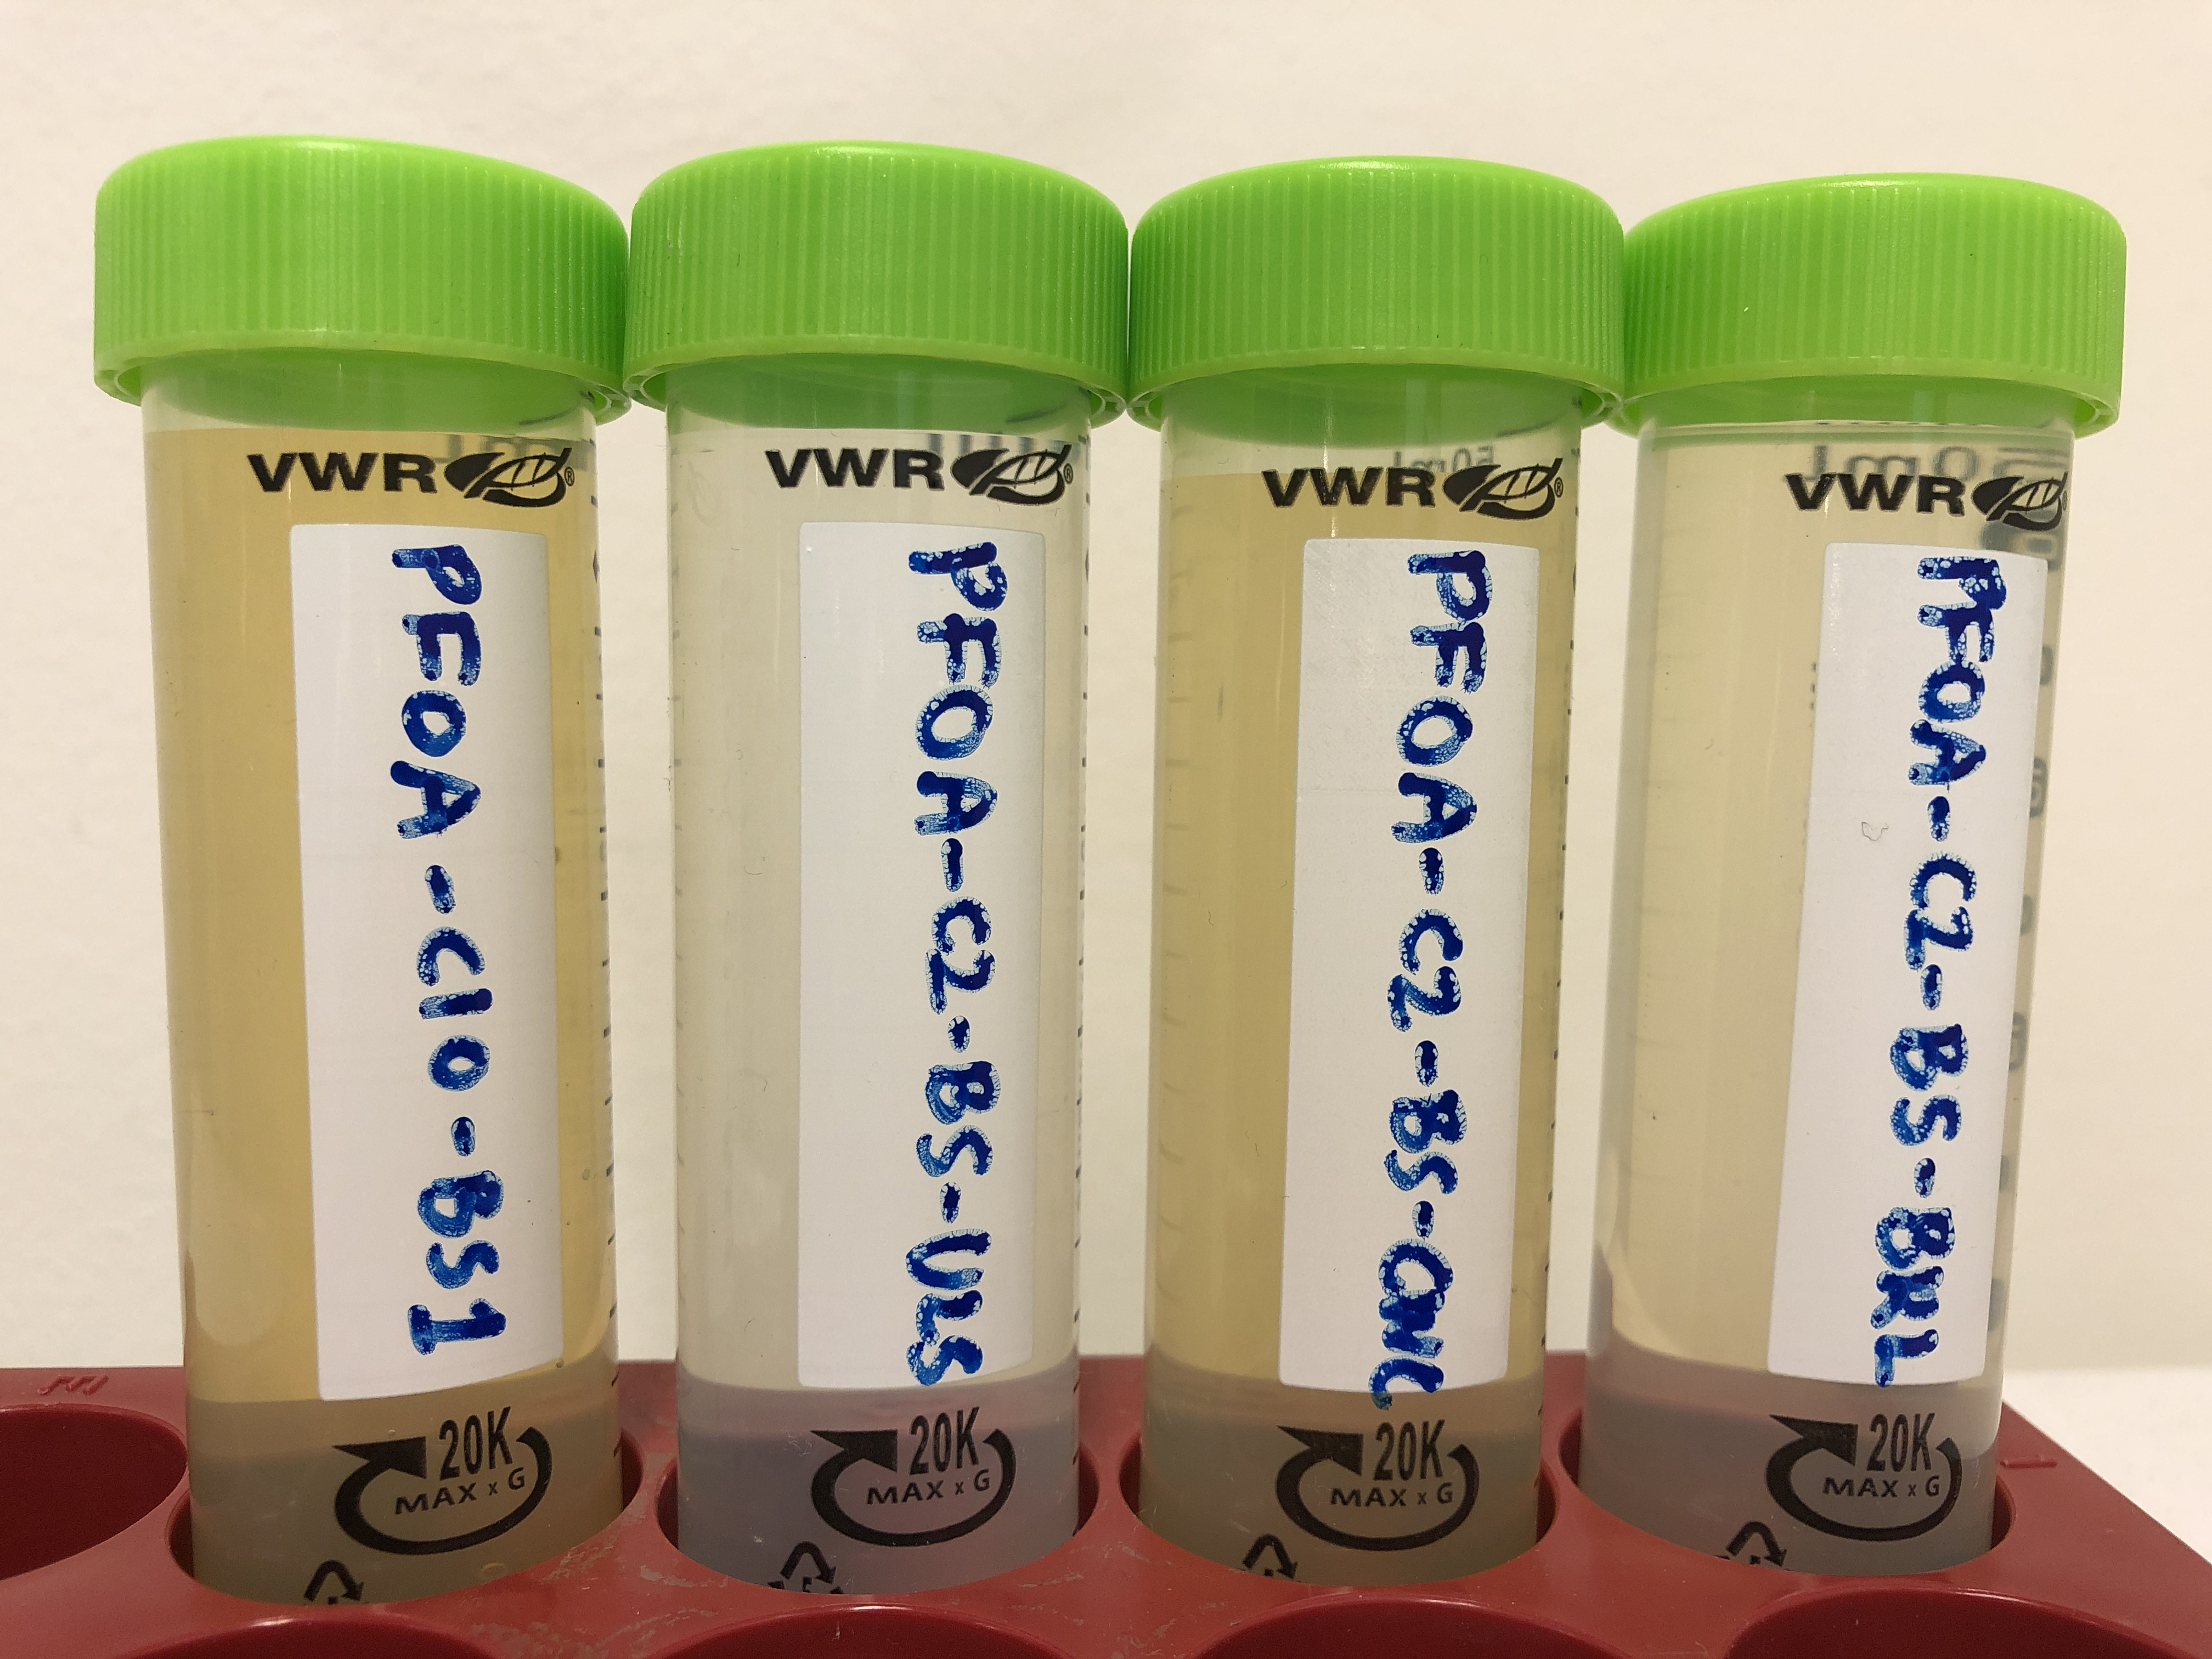
\includegraphics[width=0.45\textwidth]{Bilder/Samples/Filtrate_DOC.JPG}
}
\hfill
\subfloat[\label{subfig:precip}]{%
  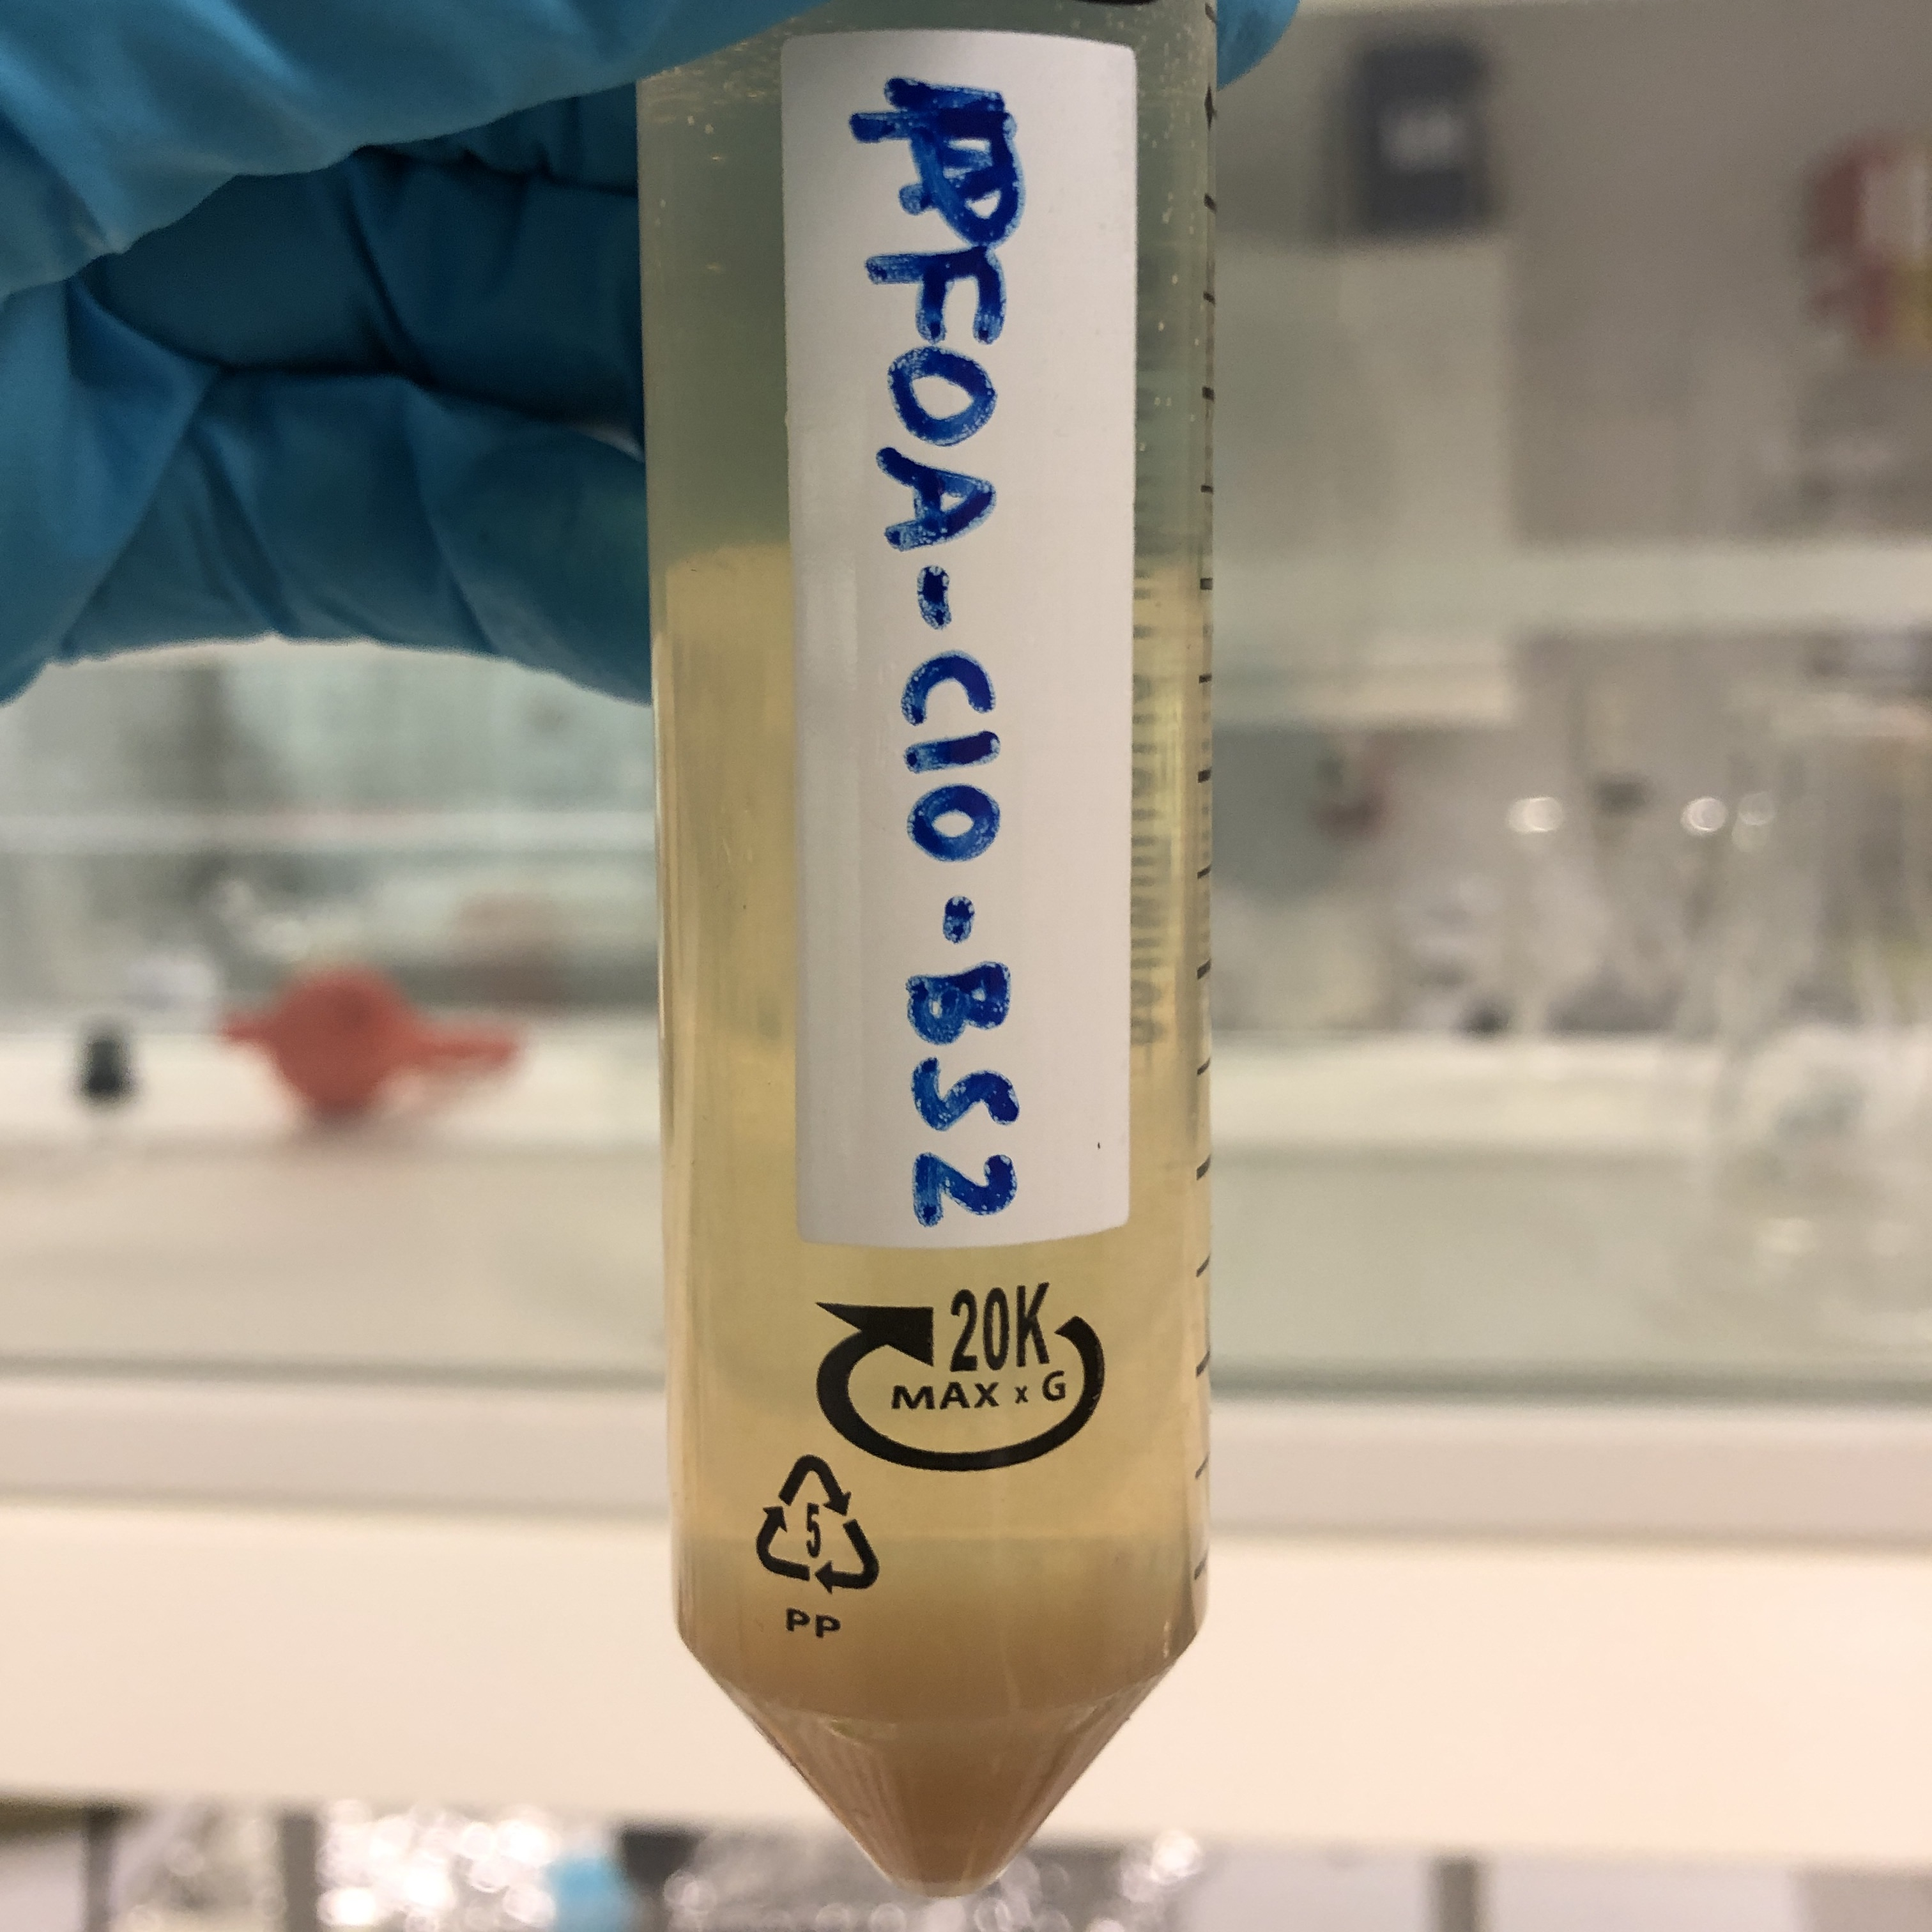
\includegraphics[width=0.45\textwidth]{Bilder/Samples/Precipitation.jpg}
}
\caption{(a) Color of filtrate for each biochar batch test. From left to right: soil only, soil+ULS, soil+CWC, and soil+BRL. (b) Precipitation observed when filtered soil samples were adjusted to pH 3 with 1 M acetic acid.}
\label{fig:DOC_tubes}
\end{figure}

\begin{figure}[htb]
    \centering
    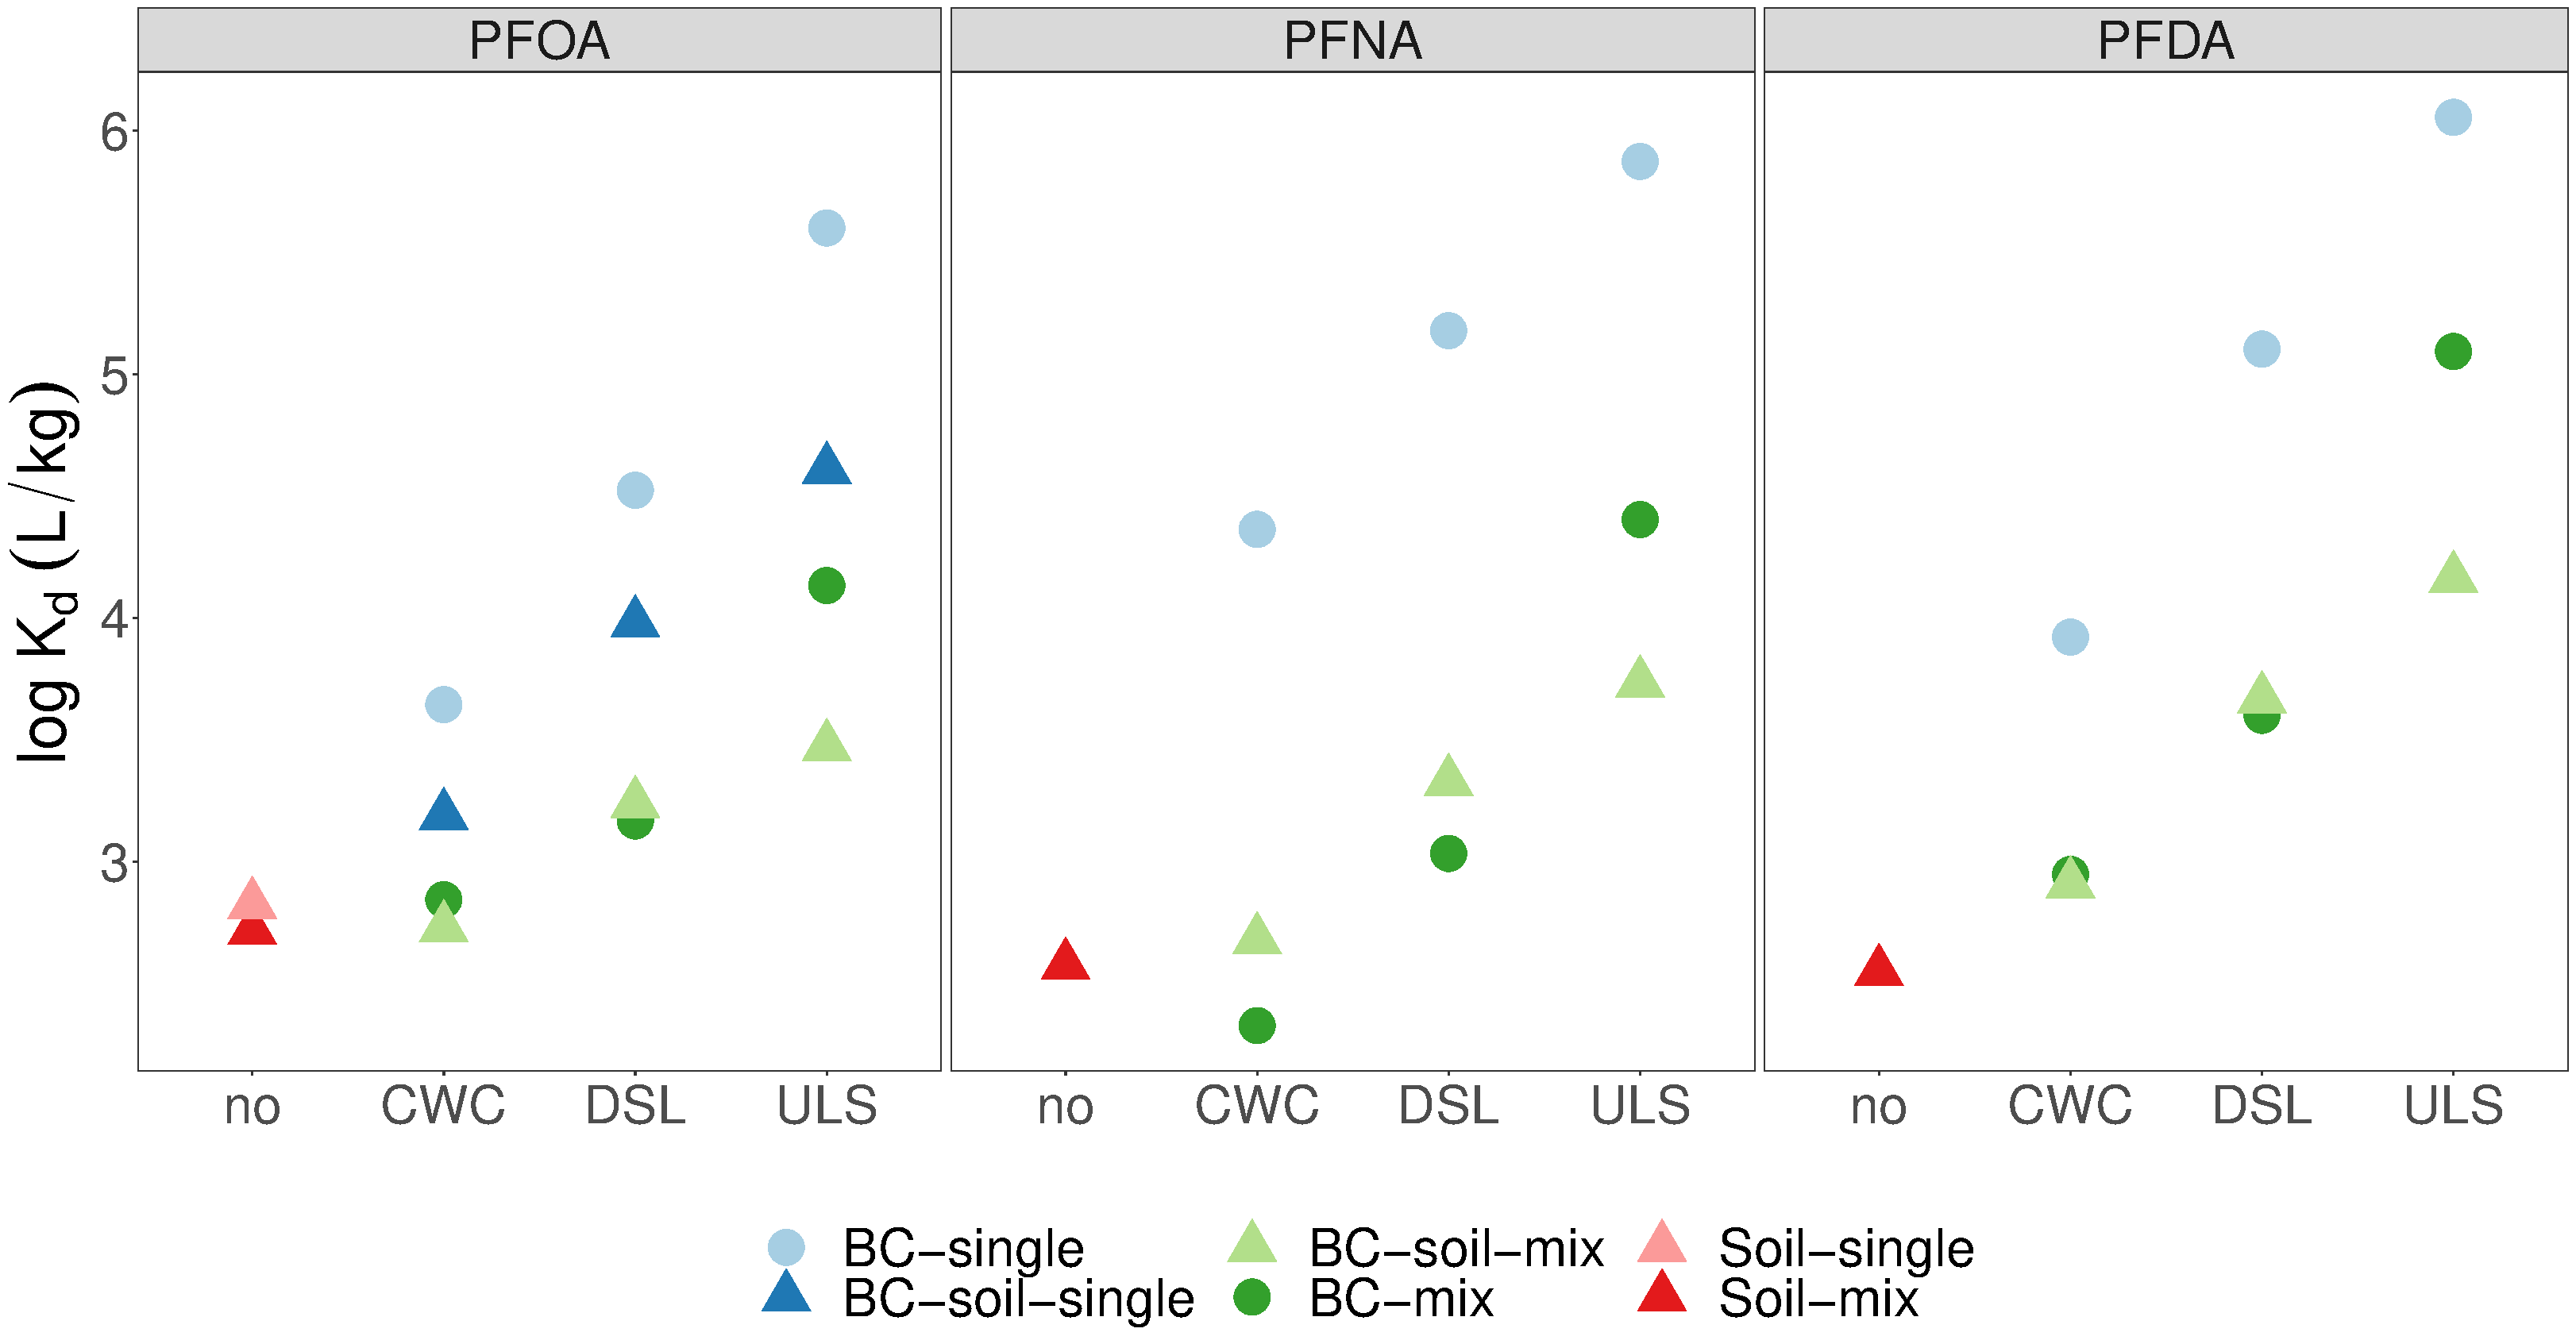
\includegraphics[width=0.8\textwidth]{R/figs/C10.pdf}
    \caption{Sorption attenuation for each TC by soil and/or competing congeners at SC10 (191, 330, 117, 1 953, 1 409, and 3 830 \textmu g L\textsuperscript{-1} for C5-C10, respectively). The error bars represent the standard deviation of $log~K_d$ for the cocktail batch tests performed in triplicate (not included). The single-compound $log~K_d$'s are single points.}
    \label{fig:C10}
\end{figure}

\begin{figure}[htb]
    \centering
    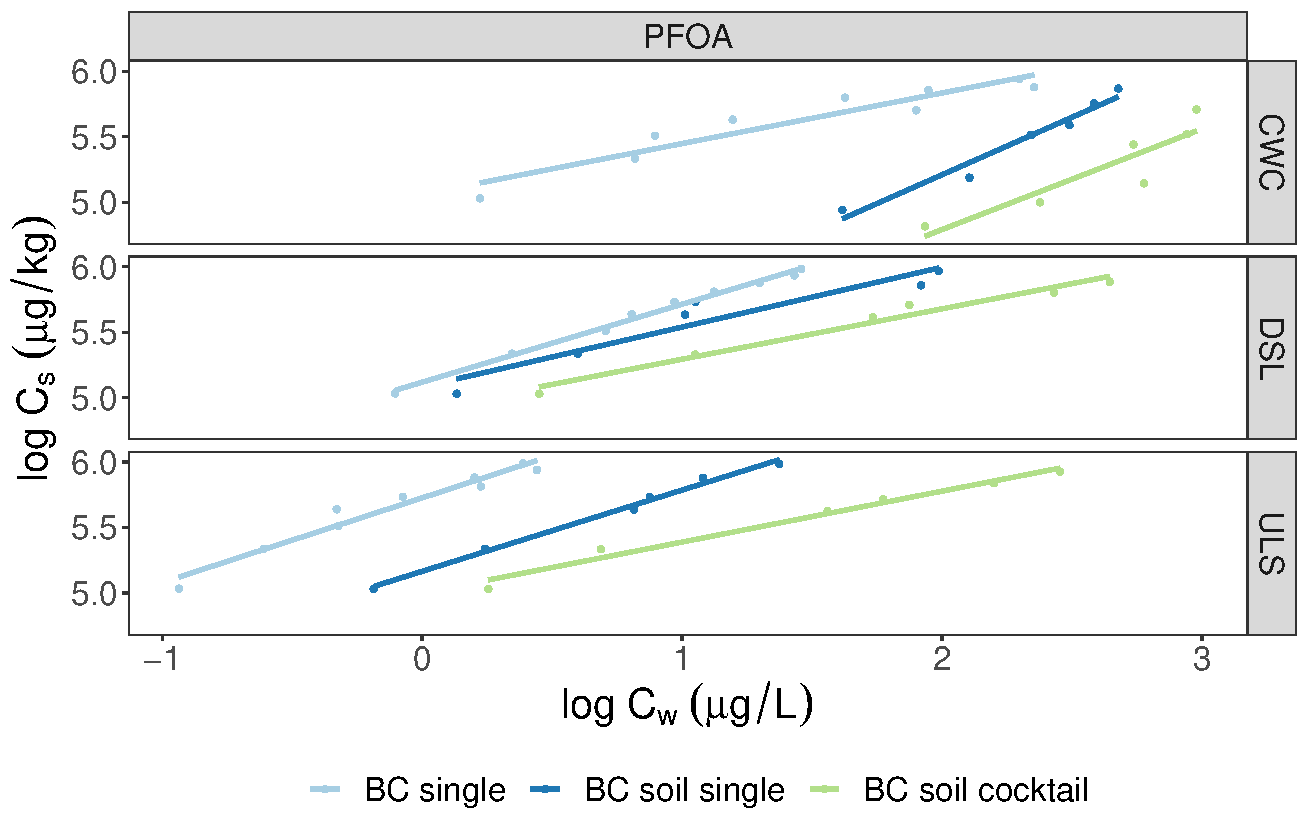
\includegraphics[width=0.8\textwidth]{R/figs/Attenuation_isotherms_PFOA.pdf}
    \caption{Sorption isotherm comparison for PFOA single-compound spike in biochar (BC single), single-compound spike in soil-biochar (BC soil single), and PFOA spiked in a cocktail in soil-biochar showing attenuation by soil and competing congeners.}
    \label{fig:PFOA_attenuation}
\end{figure}

\begin{figure}[htb]
    \centering
    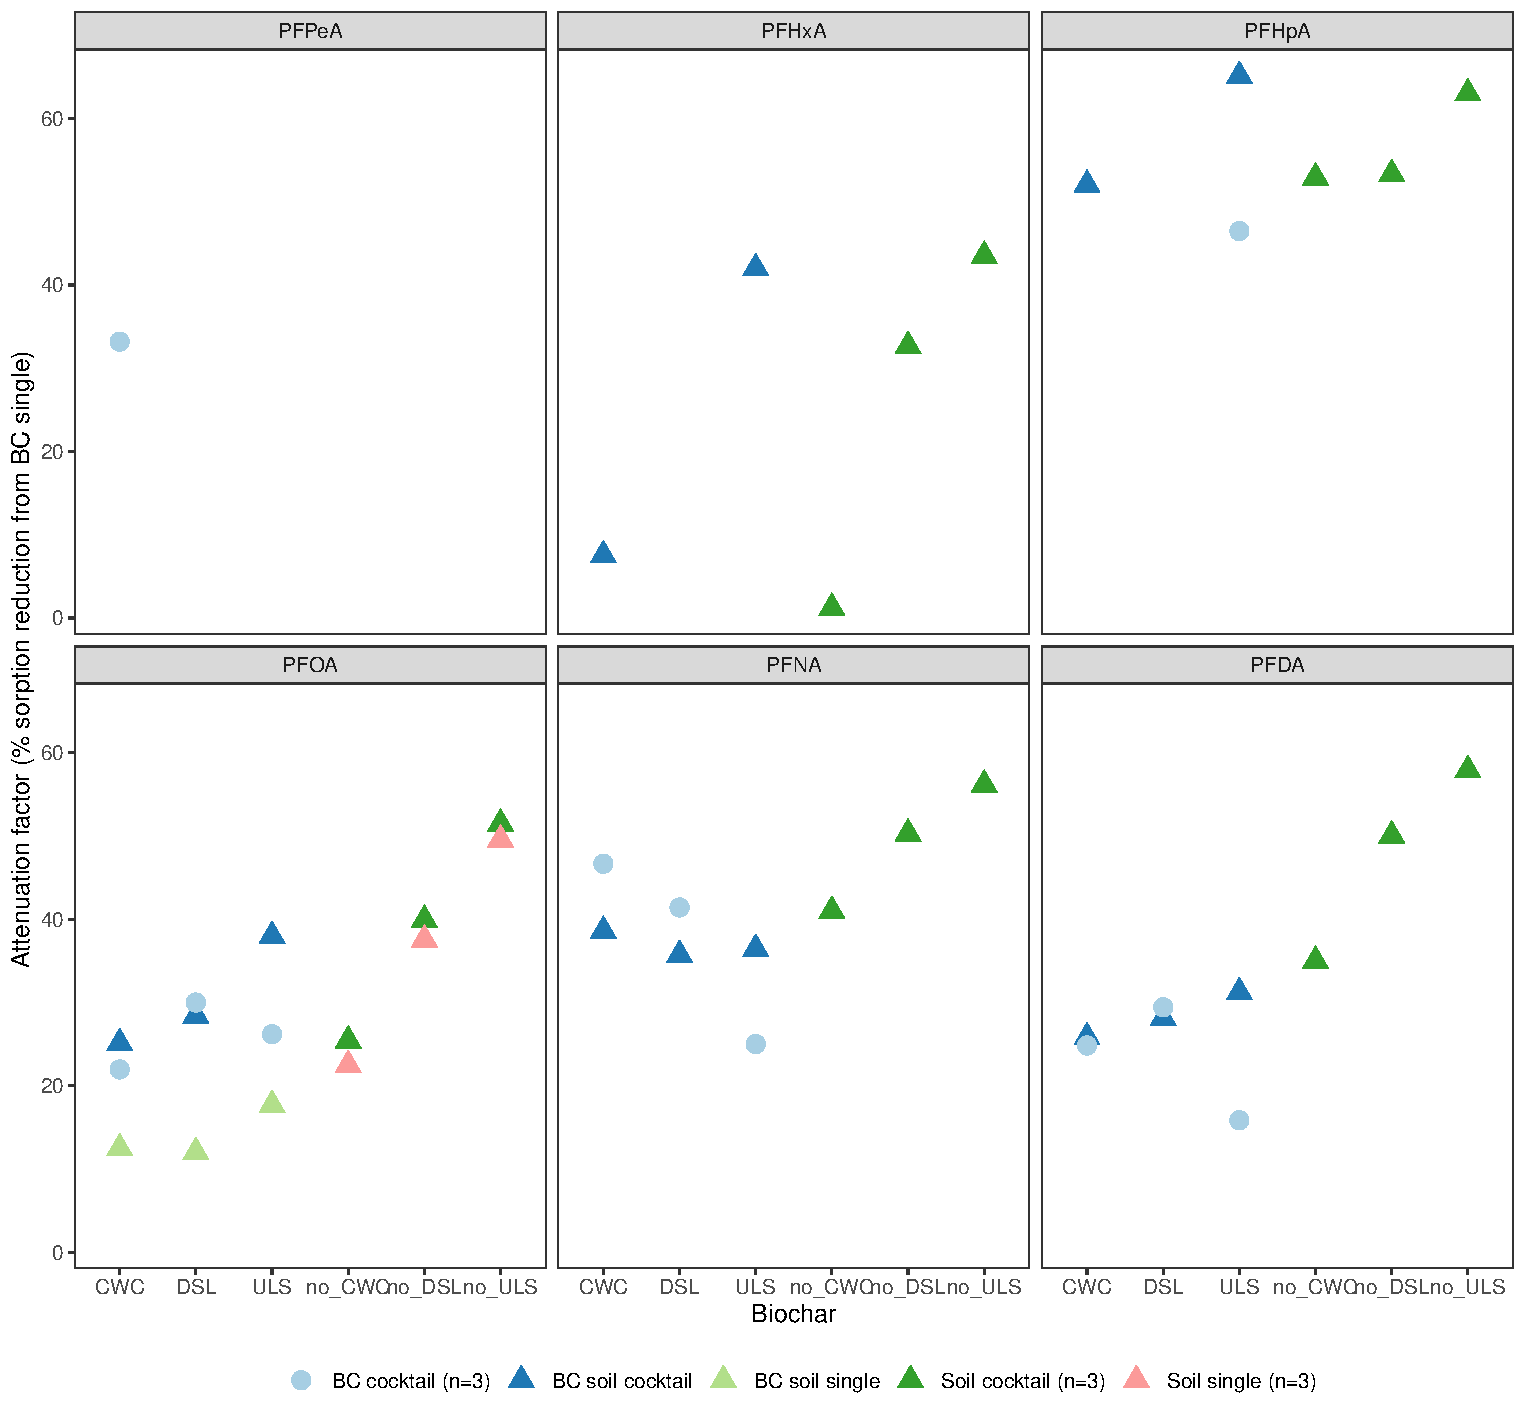
\includegraphics[width=0.8\textwidth]{R/figs/Attenuation_factors_C10.pdf}
    \caption{Attenuation factors at C10 calculated as \% reduction in $K_d$ from BC single. BC cocktails are spiked with 7.8 mg/L total PFCA and BC soil cocktails with 10.8 mg/L , the difference is due to analytical uncertainty and will be discussed assuming the that the spike concentrations are similar. See \cref{tab:spikeConcentrations} for spike concentrations used for each PFCA in the single-spike and cocktail-spike batch tests.}
    \label{fig:attenuation_factors}
\end{figure}


\begin{table}
\centering
\caption{Competition factor at SC10 (\cref{tab:spikeConcentrations}) for each compound and biochar. Competition factor is defined as K\textsubscript{d,single}/K\textsubscript{d,mix})$\times$100\%.}
\begin{threeparttable}
\label{tab:competition}
\begin{tabular}{lrrr}
\toprule
 & \multicolumn{3}{c}{Competition factor \%} \\ \cmidrule(l){2-4}
 & CWC & ULS & DSL \\ \midrule
PFPeA & 8.2 & \textsuperscript{*} & \textsuperscript{*} \\
PFHxA & \textsuperscript{*} & 2.3 & \textsuperscript{*} \\
PFHpA & \textsuperscript{*} & 0.2 & \textsuperscript{*} \\
PFOA & 15.8 & 3.4 & 4.4 \\
PFNA & 0.9 & 3.4 & 0.7 \\
PFDA & 10.6 & 10.9 & 3.1 \\ \bottomrule
\end{tabular}
\begin{tablenotes}
\item \textsuperscript{*} Amount in filtrate exceeded the amount spiked due to analytical uncertainty.
\end{tablenotes}
\end{threeparttable}
\end{table}

\subsection{Sorption non-linearity}
$n_F$ is a dimensionless empirical parameter that represents sorption linearity. All isotherms experience sorption site saturation at increasing concentrations indicated by $n_F<1 $ (\cref{tab:summary_stats_single}, which is consistent with the Freundlich model and other studies where sorption to biochar sees $n$-values typically around 0.3-0.7 \citep{Cornelissen2005}. From other studies, $K_F$ increases and $n_F$ decreases with decreasing O/C, H/C, and N/C ratios \citep{Cornelissen2005}. However, this study $K_F$ decreases with decreasing O/C, H/C, and N/C ratios, and no clear trend is seen for $n_F$ \cref{subfig:n}. Meanwhile, it does seem like the nonlinearity coefficients for CWC are more stable with increasing chain lengths than ULS and DSL. Additionally, comparing $n$ across compound isotherms does not make sense due to different spike concentrations being used for each compound. \citep{yin2022insights} suggests that electrostatic interactions between PFCAs and sediment can contribute to further enhancement of saturation of the adsorption sites and that intermolecular electrostatic repulsion between the individual molecules could also result in nonlinear sorption \citep{higgins2006sorption,yin2022insights}.

\citep{yin2022insights} attributes non-linear sorption to three explanations: 1) complex composition of biochar with negative, positive and neutral charges within same matrix, 2) successive saturation of adsorption sites, 3) electrostatic interactions between the PFASs and sediment, 4) electrostatic repulsion from negatively charged carboxylate groups. 

Sorption non-linearity ($n<1$) occurs due to the complex composition of sediment/biochar with both positive and negative charges contributing to either attraction or repulsion, as well as hydrophobic surfaces, and indicates successive saturation of these adsorption sites \citep{yin2022insights}.  

For the short-chain compounds (PFPeA and PFHxA), Correlations are poor which results in higher standard errors and slopes that are unrealistic (PFHxA-DSL: n=1.11 and PFHpA-ULS: 1.08). Possible explanations for the poor correlations for PFPeA and PFHxA are poor biochar affinity, but the standard error is also large so that the isotherm may actually be linear ($\pm$ 0.11 for both). For PFPeA- and PFHxA-CWC, it appears that CWC sorption sites have been saturated since most points center around the same area, which means that CWC reaches sorption maximum at $~$4 000 $\mu g~kg^{-1}$. However, four points are insufficient to conclude that CWC has the lowest affinity and capacity to sorb short-chain PFCAs. The CWC isotherms had the widest concentration intervals for $C_w$, which can be explained by CWC being the weakest sorbent of the three biochars studied, resulting in higher aqueous concentrations than for the sludge biochars. 

\subsubsection{Isotherm concentration range}
ULS and DSL gave isotherms typically across 0-1.5 orders of magnitude, which indicates that either higher spike concentrations or a lower BC dosage should have been used for the batch tests and that the sludge biochars have a higher sorptive capacity compared with CWC. The batch tests were spiked at 10 concentrations over four orders of magnitude where the lowest concentration was aimed at being close to the instrumental LOQ. Poor signals were achieved for the SC1 points and were removed from the data analysis to improve the certainty of the regression analysis. By doing this the spike concentration interval was reduced to two orders of magnitude \cref{tab:spikeConcentrations}. The concentration range achieved was an average of 1.3 log units for the batch test filtrate, in contrast to the desired concentration range over 4 log units. In retrospect, spike concentrations at each log unit should have been selected instead of spreading the ten concentrations evenly across the concentration range. Gaining valid points across a wider concentration range could affect the $n_F$-value acheived. 

%%%%%%%%%%%%%%%%%%%%%%%%%%%%%%%%%%%%%%%%%%%%%%%%%%%%%%%%%%%%%%%%%%%%%%%%%%%%%%%%%%%%%%%%%%%%%%%%%%%%%%%%%%%%%%%%%%%%%%%%%%%%%%%%%%%%%%%%%%%%%%%%%%%%%%%%%%%%%%%%%%%%%%%%%%%%%%%%%%%%%%%%%%%%%%%%%%%%%%%%%%%%%%%%%%%%%%%%%%%%%%%%%%%%%%%%%%%%%%%%%%%%%%%%%%%%%%%%%%%%%%%%%%%%%%%%%%%%%%%%%%%%%%%%%%%%%%%%%%%%%%%%%%%%%%%%%%%%%%%%%%%%%%%%%%%%%%%%%%%%%%%%%%%%%%%%%%%%%%%%%%%%%%%%%%%%%%%%%%%%%%%%%%%%%%%%%%%%%%%%%%%%%%%%%%%%%%%%%%%%%%%%%%%%%%%%%%%%%%%%%%%%%%%%%%%%%%%%%%%%%%%%%%%%%%%%%%%%%%%%%%%%%%%%%%%%%%%%%%%%%%%%%%%%%%%%%%%%%%%%%%%%%%%%%%%%%%%%%%%%%%%%

\section{Effect of biochar properties on sorption}
This section compares the distribution coefficients derived for ULS, DSL and CWC to biochar composition of main elements (C, H, O, N), trace elements (Ca and Fe), and surface area (SA) and pore volume (PV) in order to gain insights into possible sorption mechanisms. In the comparison between sorbent properties and sorption coefficients for each biochar type, PFOA, PFNA and PFDA have been used because they gave the best sorption isotherms. $log~K_F$ has been normalized to 1 $\mu g~L^{-1}$ which is used as the distribution coefficients in this discussion.

\subsection{Surface area and pore volume}

\begin{table}
\centering
\caption{Surface area (SA), pore volume (PV), elemental content (C, O, H, N) and ratios for the biochars produced for the batch tests.}
\adjustbox{max width=\textwidth}{
\label{tab:SAPV}
\begin{tabular}{llrrrrrrlllllll}
\toprule
Biochar & Pyrolysis & \multicolumn{3}{l}{N\textsubscript{2} sorption} & \multicolumn{3}{l}{CO\textsubscript{2} sorption} & \multicolumn{4}{c}{Elemental content} & \multicolumn{3}{c}{Elemental ratio} \\
sorbent & temperature & \multicolumn{3}{l}{(pores \textgreater 1.5 nm)} & \multicolumn{3}{l}{(pores 0.4-1.5 nm)} & & & & & & & \\ \cmidrule(l){3-5} \cmidrule(l){6-8} \cmidrule(l){9-12} \cmidrule(l){13-15} & (\textdegree C) & BET SA  & BJH PV & log SA/PV & DFT SA & DFT PV & log SA/PV & C & O & H & N & O/C & H/C & N/C \\
& & ($\mathrm{m^2~g^{-1}}$) & (cm\textsuperscript{3} g\textsuperscript{-1}) & ($\mathrm{m^2 cm^{-3}}$) & ($\mathrm{m^2~g^{-1}}$) & (cm\textsuperscript{3} g\textsuperscript{-1}) & ($\mathrm{m^2 cm^{-3}}$) & (\%) & (\%) & (\%) & (\%) & & & \\ \midrule
CWC & 700 & 323 & 0.017 & 3.21 & 683 & 0.186 & 3.54 & 91.4 & 5.50 & 1.01 & 0.69 & 0.06 & 0.01 & 0.008       \\
ULS & 700 & 128 & 0.126 & 2.80 & 165 & 0.047 & 3.57 & 29.6 & 57.1 & 1.24 & 1.13 & 1.9  & 0.04 & 0.04        \\
DSL & 700 & 110 & 0.111 & 2.80 & 87  & 0.027 & 3.51 & 13.5 & 61.4 & 1.05 & 0.82 & 4.6  & 0.08 & 0.06       \\ \bottomrule
\end{tabular}}
\end{table}

\subsubsection{Pore size distribution of small pores}
\cref{tab:SAPV} shows the total surface area (SA, m\textsuperscript{2}/g) and pore volume (PV, cm\textsuperscript{3}/g) for the three biochars used in the sorption experiments in this study. For small pores (0.4-1.5 nm, CO\textsubscript{2} sorptiometry), SA of CWC was $\sim$six times higher than ULS and DSL (165 and 87  m\textsuperscript{2} g\textsuperscript{-1}, respectively), and PV also followed the same order. Previous research agree that large internal surface area and pore volume are desirable for strong sorption of organic contaminants because it increases available sorption sites \citep{ahmed2020per,Hale2016}. The high SA and PV of CWC suggests that this biochar has the highest fraction of available sorption sites compared to ULS and DSL within the micropore range ($\le$ 2 nm). However, as graphed in \cref{fig:PZD_small}a-c, it becomes becomes evident that nearly 80\% of the SA and 60\% of the PV of CWC is located in nanopores $<$ 0.6 nm. These pores become nearly inaccessible to the adsorbate molecules because the perfluorinated chains are quite large and rigid, preventing them from entering pores that are too small, and if managing to enter, they have difficulties adapting its shape to the pore wall to sorb strongly due to steric hindrance. Additionally, molecular size increases with chain length, which makes it even more difficult for long-chain PFASs to diffuse into the smallest pores. 

\cref{tab:molecsize} lists effective cross-sectional diameter ($D_{eff}$) and maximum diameter ($D_{max}$) of each TC (the definitions of $D_{eff}$ and $D_{max}$ are illustrated in \cref{fig:molecularSize}). PFCAs C5-C10 range from 0.45-0.72 nm $D_{eff}$ and 0.96-1.54 nm $D_{max}$. Maximum sorption is acheived when the molecular dimensions of the PFAS congeners match the pore size and shape \citep{Hale2016}. Since the PZD within the CO\textsubscript{2}-range is dominated by pores $<$0.6 nm for CWC, ULS, and DSL, sorption of PFPeA, PFHxA, and PFHpA is only possible if the congeners enter the pores at the exact right angle, whereas PFOA, PFNA, and PFDA will experience size exclusion, and the pores are easily blocked by large molecules. Therefore, sorption of PFAS in the CO\textsubscript{2}-range is insignificant and cannot explain the differences in $log~K_F$ between biochar types, especially since strongest sorption was measured for long-chain PFCAs (PFOA, PFNA, and PFDA).

%consider removing log SA/PV graph, and rather wait with this discussion for the large pores. There are only minor differences in SA/PV ratio between the biochars (cumulative ratios: 3 674, 3 502, and 3 206 m\textsuperscript{2} cm\textsuperscript{-3} for CWC, ULS, and DSL respectively), which means that despite CWC being far more numerous in nanopores than ULS and DSL, the structure of these pores are similar, and the highest proportion of nanopores for all three biochars are $<$0.6 nm.

\begin{figure}[htb]
    \centering
    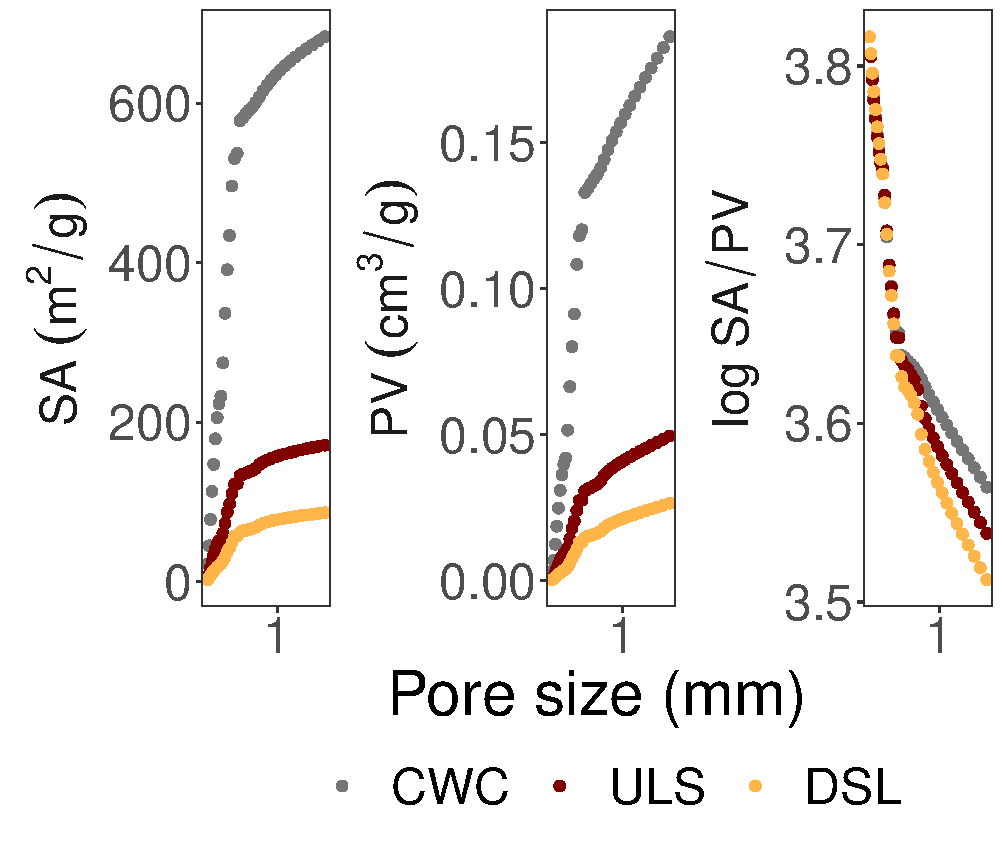
\includegraphics[width=\textwidth]{R/figs/PZD_SAPV_C_small_plot.pdf}
    \caption{Cumulative pore size distribution for pores 0.4-1.5 nm using DFT.}
    \label{fig:PZD_small}
\end{figure}

\begin{table}
\caption{Effective cross-sectional diameter ($D_{eff}$) and maximum diameter ($D_{max}$) of TCs interpolated and extrapolated by linear regression from calculations performed by \cite{inoue2012size} on PFOA and other PFCAs with chain lengths 11-18.}
\centering
\begin{threeparttable}
\label{tab:molecsize}
\begin{tabular}{llll}
\toprule
Compound & CF\textsubscript{2} & $D_{eff}$ & $D_{max}$ \\ 
& chain & (nm) & (nm) \\ \midrule
PFPeA & 5  & 0.45  & 0.96  \\
PFHxA & 6  & 0.50  & 1.08  \\
PFHpA & 7  & 0.56  & 1.19  \\
PFOA\textsuperscript{*} & 8 & 0.61 & 1.36 \\
PFNA & 9 & 0.67 & 1.42  \\
PFDA & 10 & 0.72 & 1.54  \\ \bottomrule                                    
\end{tabular}
\begin{tablenotes}
\item \textsuperscript{*} Value from \cite{inoue2012size}
\end{tablenotes}
\end{threeparttable}
\end{table}

\begin{figure}
    \centering
    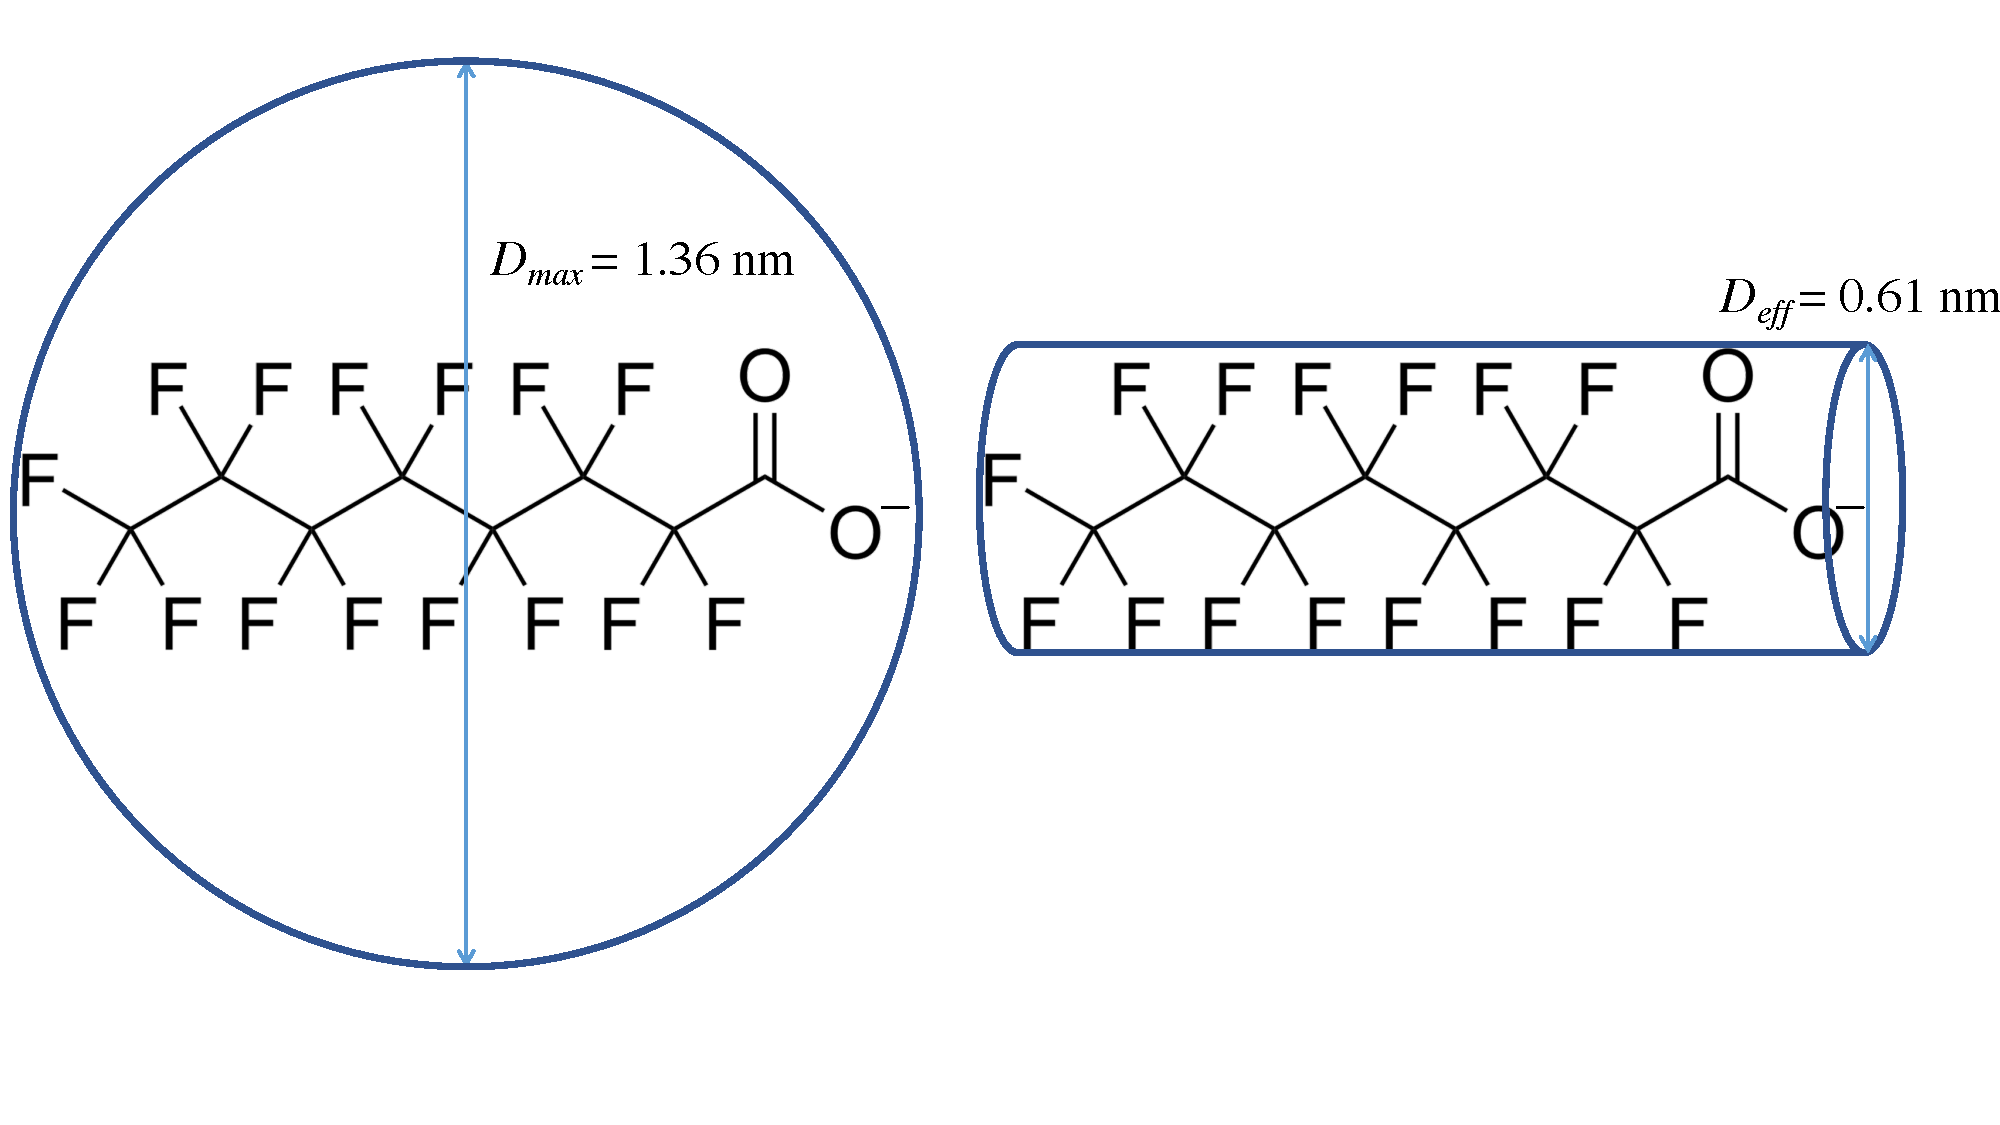
\includegraphics[width=0.8\textwidth, trim={0 2cm 0 0},clip]{Diagrams/Molecular_size.pdf}
    \caption{Definition of effective cross-sectional diameter ($D_{eff}$) and maximum diameter ($D_{max}$) shown for PFOA.}
    \label{fig:molecularSize}
\end{figure}

\subsubsection{Pore size distribution of large pores}
Similar to the trend for small pores, CWC also had the largest cumulative SA for pores $>$1.5 nm (323 m\textsuperscript{2} g\textsuperscript{-1}) versus 110 and 128 m\textsuperscript{2} g\textsuperscript{-1} for DSL and ULS, respectively. \cref{fig:PZD_large}a shows that the highest proportion of SA is allocated to pores between 1.5-5 nm for all three biochar samples. ULS had the highest cumulative PV (0.126 cm\textsuperscript{3} g\textsuperscript{-1}), whereas PV for CWC was one order of magnitude lower (0.017 cm\textsuperscript{3} g\textsuperscript{-1}). Further, the development of PV with pore size in \cref{fig:PZD_large}b shows a clear distinction between CWC and the two sewage sludge biochars. CWC has most of its PV in pores $<$3 nm, whereas ULS and DSL have volumes that increase steadily up to the maximum pore size of 35 nm. This difference becomes important when interpreting a new parameter, the SA/PV ratio, which is graphed in \cref{fig:PZD_large}c. The SA/PV better indicates the spatial arrangement of pores, where a low ratio reflects pores of maximum sorption volume. Here, ULS and DSL have low and equivalent log SA/PV ratios of 2.8 compared to CWC, which has a higher ratio of 3.21 (\cref{tab:SAPV}). Previous studies are consistent in concluding that a large internal surface area and pore volume of adsorbents is one of the most important parameters achieving high sorption capacity of PFAS \citep{du2014adsorption,Sormo2021,Hale2016,ahmed2020per}. Likewise, the results from this study provides clear indications that a low SA/PV ratio can be used to explain higher sorption capacity of ULS and DSL. Since the pores of CWC consists almost exclusively of pores $<$3 nm, whereas ULS and DSL have pores of larger size, this is the most plausible explanation for why CWC is the weakest sorbent among the three samples in this study. The shift observed by comparing SA and PV together demonstrates the importance of considering both pore size \textit{and} surface area when evaluating available sorption sites on biochar.

Since ULS and DSL have nearly equivalent SA/PV ratios, another parameter is needed to explain why ULS is a better sorbent than DSL in this study (\cref{fig:PZD_large}c). Apart from SA and PV, carbon content has shown to be a good predictor of sorption affinity to PFAS from previous literature \citep{Hale2016}. A clear distinction in pore structure emerges by by normalizing the SA/PV ratio for C-content, whereby ULS consists of 29.6 \% C versus 13.5 \% for DSL (\cref{fig:PZD_large}d). ULS has a lower (SA/PV)/C ratio (CALCULATE!!), which means that the pore walls of ULS consists of a higher percentage C making the pore walls more hydrophobic and enhances sorption affinity of PFAS. 

\cref{fig:Kd_SAPV_C} also shows that individually, C and SA/PV does not explain sorption, but together they do.  

In summary, difference in sorption between CWC, DSL, and ULS can be explained by 1) difference in nanopore and micropore structure, where a higher number of large micropores signified by low SA/PV ratio is more ideal for sorption of long-chain PFASs such as PFOA, PFNA, and PFDA, and 2) a higher proportion of carbon in the pore wall matrix further enhances sorption by creating more hydrophobic sorption surfaces. Since the conclusions drawn for the sorption mechanisms contributing to PFCA sorption is based on only three biochar samples, further research within this area should test if a higher sample size comply with the suggestion that pore size size and structure is the most important determinant for sorption of organic contaminants. 

\begin{figure}[htb]
    \centering
    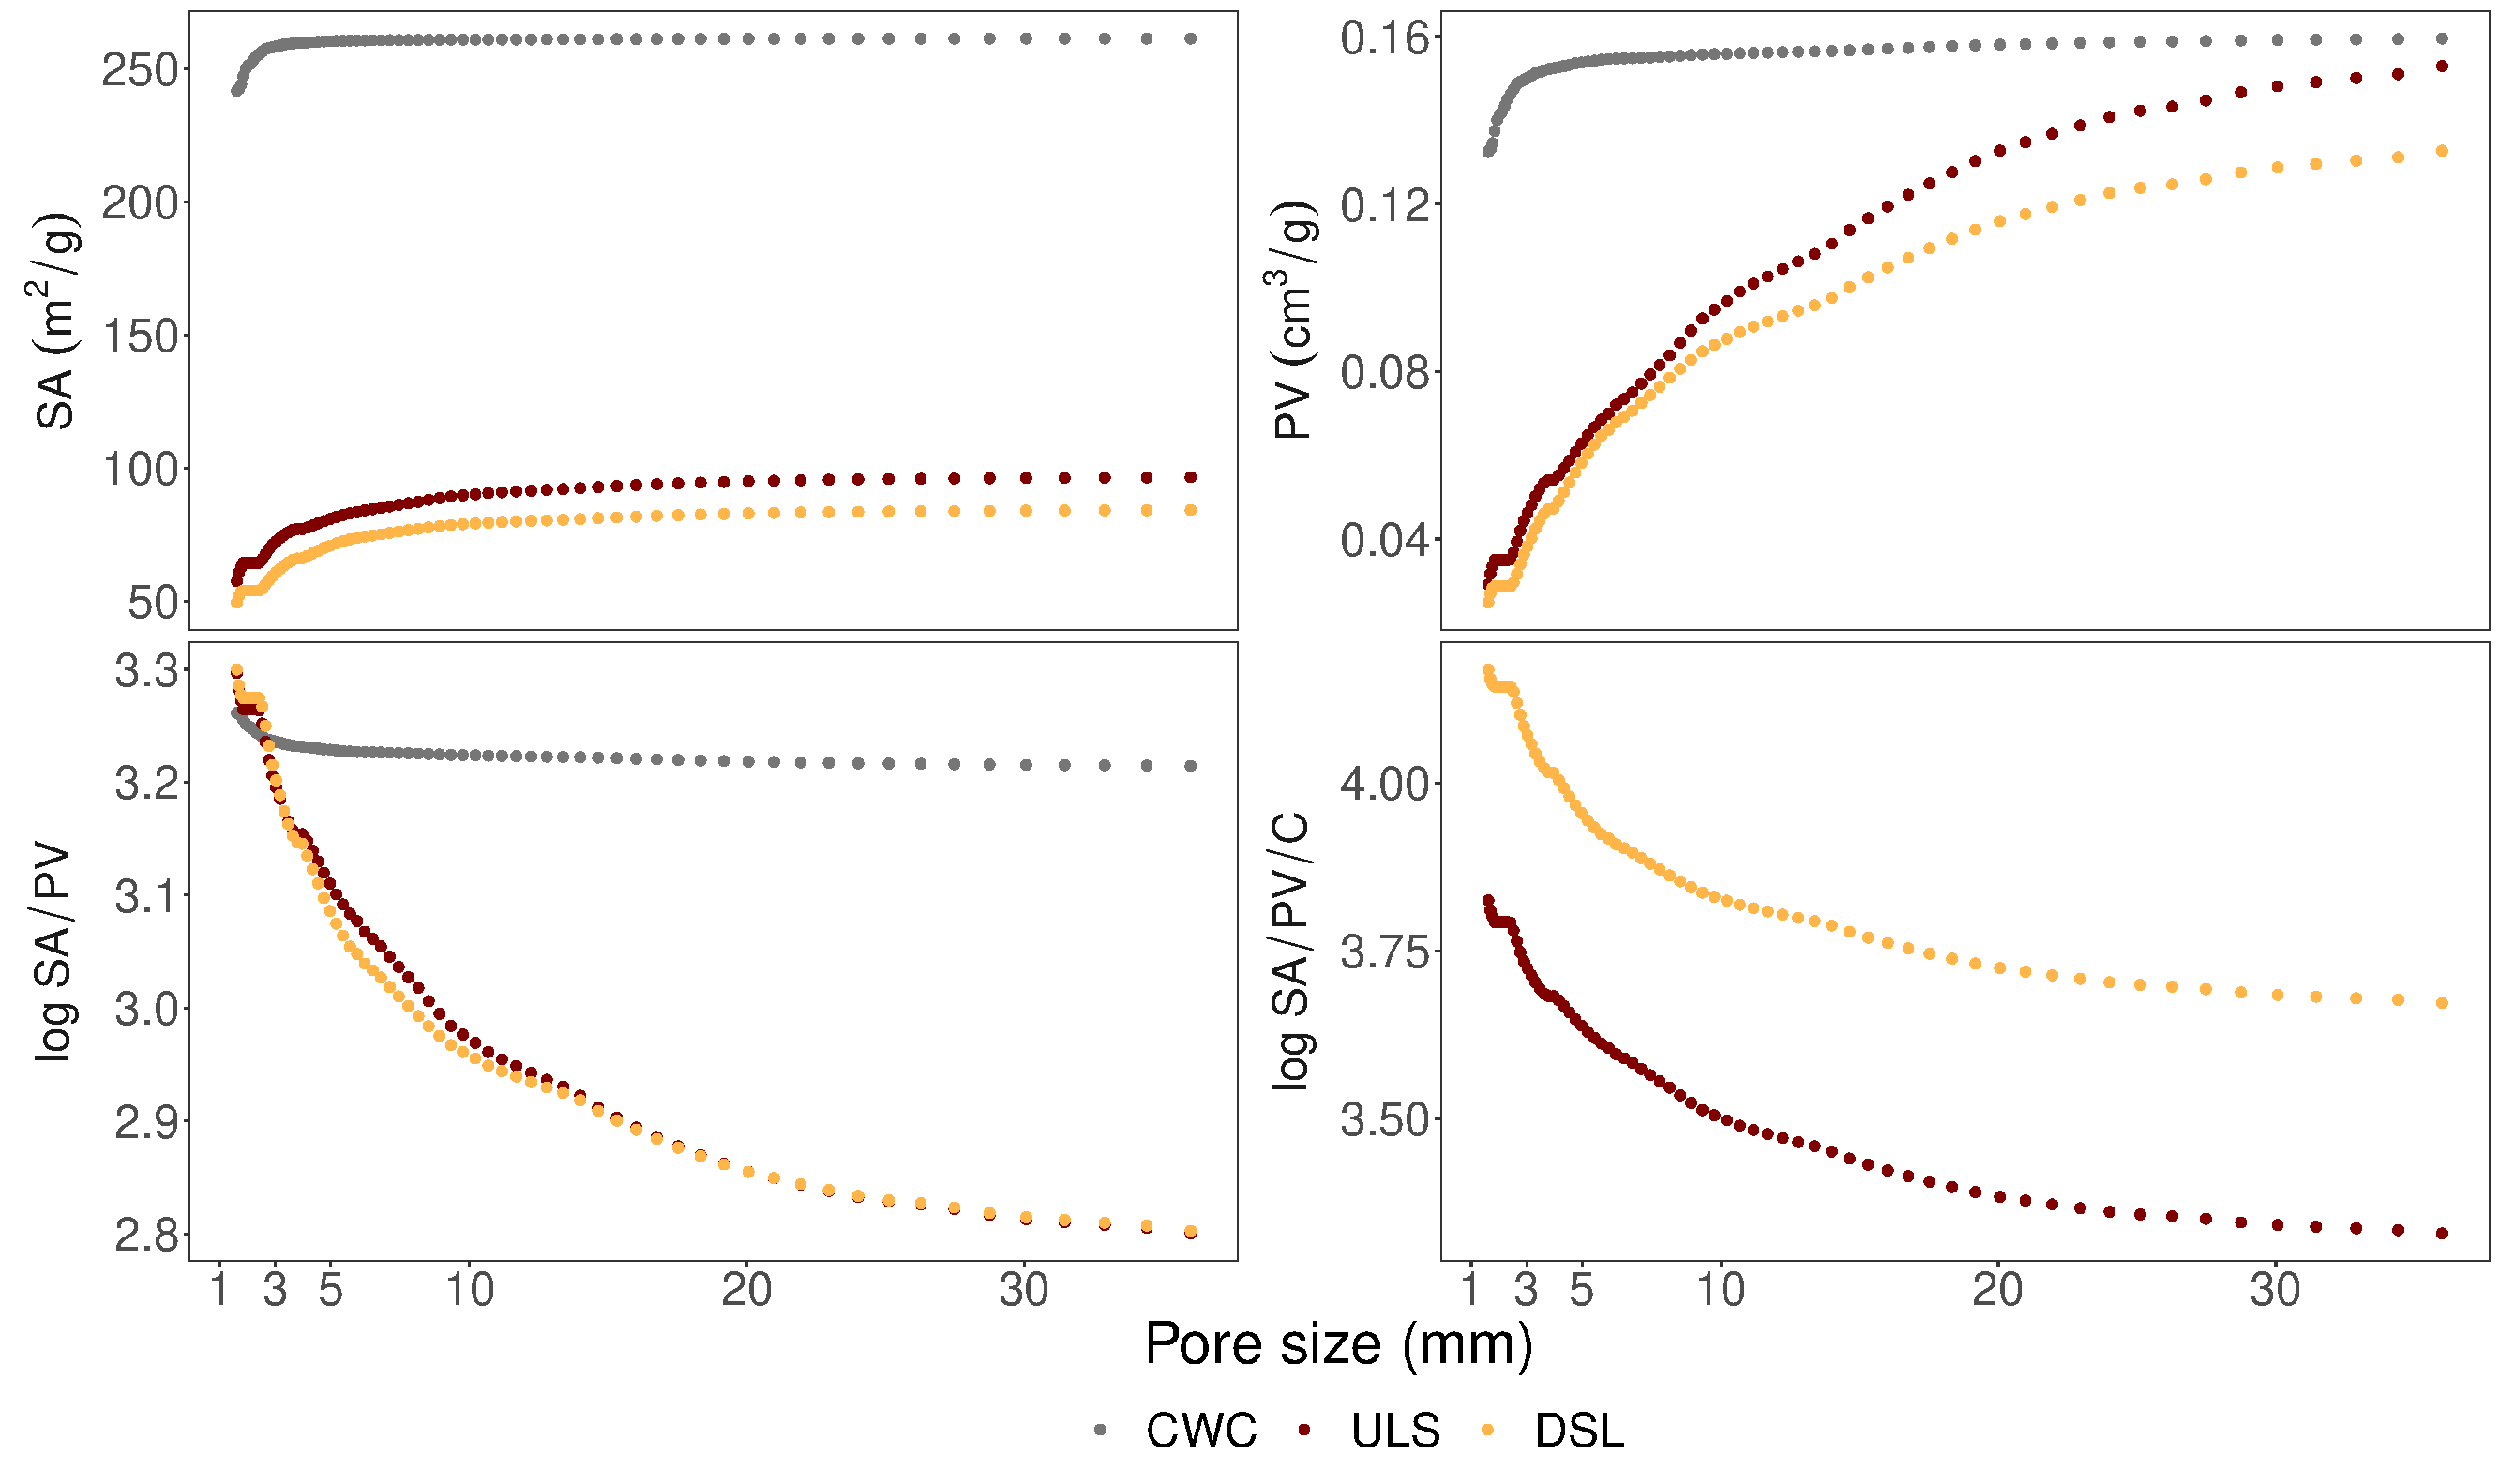
\includegraphics[width=\textwidth]{R/figs/PZD_SAPV_C_large.pdf}
    \caption{Cumulative pore size distribution for pores $>$ 1.5 nm using DFT theory. (a) Surface area, (b) pore volume, (c) SA/PV ratio for pores $>$1.5 nm normalized to carbon content (g C/g BC). (d) A lower SA/PV/C ratio indicates a higher degree of C in the pore wall matrix.}
    \label{fig:PZD_large}
\end{figure}


\subsection{Surface chemistry}
Based on feedstock type for the three biochars studied in this thesis, carbon content of the biochars follows the expected trend, CWC \textless ULS \textless DSL with 91.4\%, 29.6\% and 13.5\%, respectively (\cref{tab:SAPV}). Oxygen content was highest for DSL and ULS (61.4 and 57.1 \% respectively) compared to 5.5 \% for CWC. CWC has a low O/C and H/C ratio (\textless 1) whereas ULS and DSL have ratios \textgreater 1. A low H/C and O/C ratio is associated with high degree of aromaticity and few functional groups. This shows that the CWC matrix is dominated by aromatic carbon whereas ULS and DSL are dominated by oxidized carbon resulting in a more hydrophobic surface of the high-C biochar. A high degree of aromaticity have been reported in previous literature to be important for sorption of hydrophobic organic contaminants such as PAH's \citep{Cornelissen2005}. However, \cite{du2014adsorption} claims that optimum sorption of PFCAs occur at a higher O/C ratio with a biochar matrix consisting of more surface functional groups that are Lewis acids (hydroxyl, carbonyl, and metal-containing groups). The reason for this is that the CF chain is net negative and ion bridging is important because biochar is accompanied with high ash contents containing divalent cations. This interaction is stronger than hydrophobic interaction, which is only a compromise for PFAS which is more hydrophobic than lipophilic. 

The proportion of elements other than C, O, H and N contained in the biochar matrices is significantly lower for the clean wood biochar (1.4 \%) compared to the sludge biochars (10.9 and 23.2 \%), containing a greater mixture of other elements. Total elemental composition of the biochars is given in \cref{appSec:elements}. The results from this study is in contrast to literature \citep{Hale2016,Sormo2021,zhang2021sorption} that report that the sorption strength of organic compounds to biochar increases with decreasing biochar O/C and biochar H/C ratios. Thus, the higher sorption onto ULS and DSL cannot be explained by the sorbent composition of main elements alone.

\cite{du2014adsorption} summarizes that the more basic groups the adsorbents have, the more PFAS they can adsorb, which is somewhat counter intuitive when considering potential repulsion by the anionic PFCA functional group. The reason for this is that these groups are typically weak acids that are prone to be protonated at environmentally relevant pH's. A high pH-point of zero charge (PZC) therefore increases the adsorption capacity because the surface functional groups are more likely to be protonated. A high nitrogen/carbon (N/C) ratio is a predictor of amine groups, which is positively charged, where the N/C ratios for the biochars are listed in \cref{tab:SAPV}. Both ULS and DSL have higher ratios than CWC by one order of magnitude, so this could be a contributing factor to why the sewage sludge biochars are better sorbents for PFCAs. Even though total N does not indicate amine groups, this is an indication. Not much is known about what happens to proteins etc. during pyrolysis and how this affects speciation. But common is that this char type is more nutrient rich, which proves to be beneficial for sorption of PFAS in this study. 

Adsorption capacity has shown to also be related to solution pH, which is expected to increase with decreasing pH \citep{du2014adsorption}. However, in Ca and Mg-rich basic solutions, sorption can be enhanced through divalent cation bridging effect. pH varied little between all biochar-soil-water systems with an average pH of 7.18 \textpm 0.02. Conductivity was 39 \textpm 0.9 \textmu S cm\textsuperscript{-1}. Since the variance is low, pH and conductivity was not considered as factors that influence sorption of PFCAs. The conductivity of soil-water samples differed the most from the rest of the samples with a mean conductivity of 23 \textpm 0.05 \textmu S cm\textsuperscript{-1} versus a mean of 41 \textpm 0.9 \textmu S cm\textsuperscript{-1} for the biochar-water and biochar-soil-water samples. Complete pH and conductivity data is in \cref{appSec:misclab}.

\citep{zhang2013sorption}: sorption of PFAS increases with decreasing pH

\begin{table}
\centering
\caption{Mean pH and conductivity (\textmu S cm\textsuperscript{-1}) measurements for the different batch test systems (n=3). The error bars represent the standard error. BC/S/L is the biochar:soil:liquid ratio.}
\label{tab:pHcond}
\begin{tabular}{lccccc}
\toprule
 & \multicolumn{2}{c}{pH} & \multicolumn{2}{c}{Conductivity} & \\ \cline{2-5}
 & mean & std. dev & mean & std. dev & BC/S/L\\ 
\midrule
ULS & 7.10 & 0.04 & 45.70 & 3.03 & 1/0/500\\
DSL & 7.31 & 0.02 & 40.93 & 1.07 & 1/0/500\\
CWC & 7.36 & 0.07 & 46.47 & 0.70 & 1/0/500\\
ULS+S & 7.18 & 0.02 & 34.93 & 0.40 & 1/50/500\\
DSL+S & 7.14 & 0.00 & 35.73 & 1.50 & 1/50/500\\
CWC+S & 7.09 & 0.05 & 44.90 & 1.54 & 1/50/500\\
S & 7.08 & 0.05 & 23.33 & 0.87 & 0/1/10\\
\bottomrule
\end{tabular}
\end{table}

\begin{figure}[htb]
    \centering
    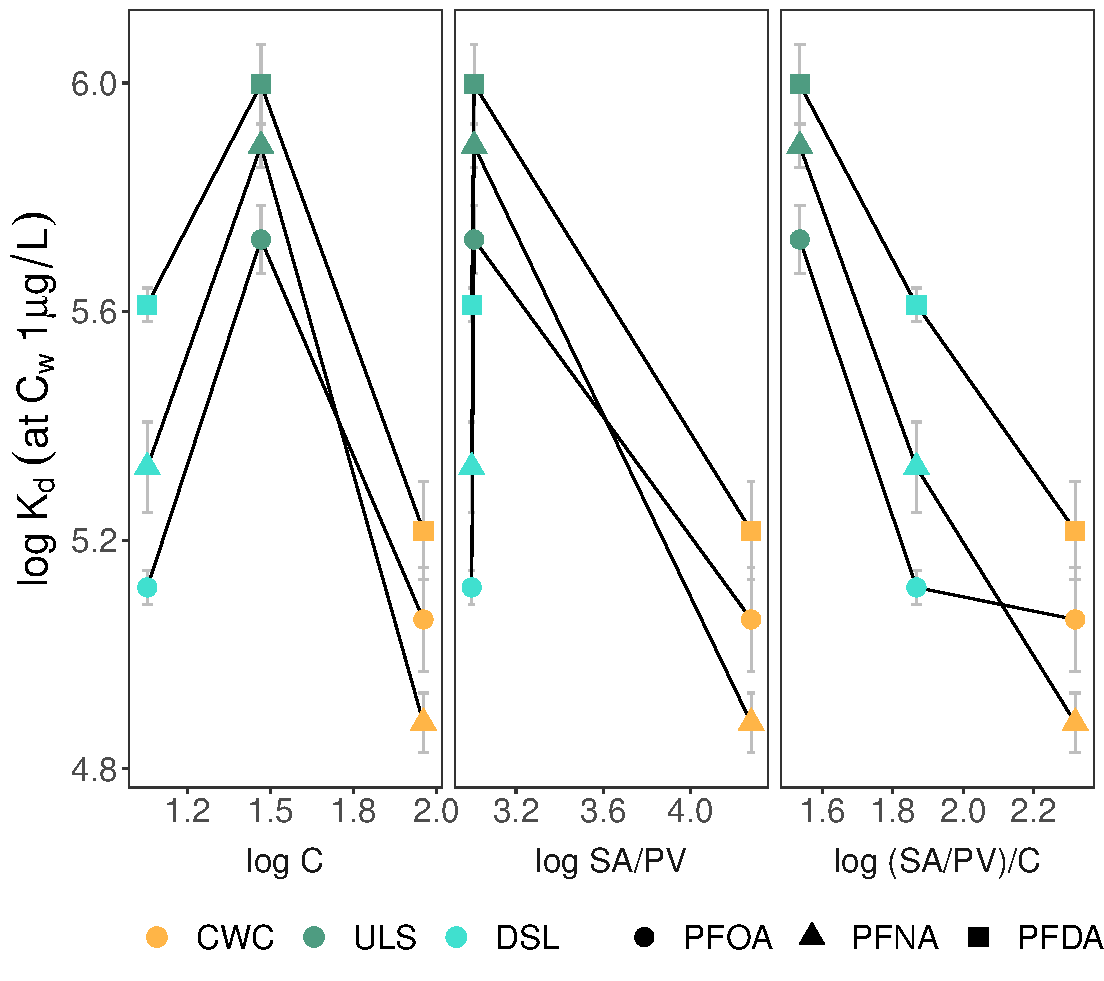
\includegraphics[width=\textwidth]{R/figs/SAPV_C_Kd1ugL_plot.pdf}
    \caption{The correlation of $log~K_d$ vs. (a) log C (b) log SA/PV (c) log (SA/PV)/C using BET for SA and BJH for PV by biomass feedstock. Error bars are the propagated standard error of $log~K_F$ and $n$.}
    \label{fig:Kd_SAPV_C}
\end{figure}


\subsection{Effect of solution chemistry}

\begin{table}
\centering
\caption{Composition of a selection of elements in the biochar samples in mg/kg.}
\label{tab:BC_mainElements}
\begin{tabular}{lllllllll} \toprule
 & Ca & Fe & K & Mg & Na & P & S & Si \\ \midrule
CWC & 8.03 & 0.13 & 4.0 & 0.91 & 0.052 & 0.41 & 0.089 & 0.17 \\
DSL & 26 & 180 & 3.7 & 4.7 & 1.8 & 8.0 & 7.2 & 0.62 \\
ULS & 21 & 23 & 6.8 & 5.3 & 2.4 & 45 & 2.9 & 1.7 \\ \bottomrule
\end{tabular}
\end{table}

\subsection{Effect of inorganic ions}
Elements that may affect sorption properties of the biochars are provided in \cref{tab:BC_mainElements}. Since ionic forms have not been analyzed, an assumption based on the total element composition must be made during the discussion of potential roles of inorganic ions for PFAS sorption. The sludge chars have expectantly the highest mineral content overall due to the heterogeneous composition of sewage sludge. 

Coexisting inorganic cations and anions complicates sorption behavior of PFCAs, where several mechanisms are involved in changing both solution and biochar surface chemistry \citep{du2014adsorption}. The presence of ions can both enhance or suppress sorption through mechanisms such as electrical double-layer compression, surface-charge neutralization, divalent cation bridging, competitive adsorption, and salting-out. The latter mechanism occurs only at high enough salt concentration and is not applicable for the present study. 

ULS and DSL are similar in earth alkali composition that gives rise to divalent ions  and CWC is one and two orders of magnitude lower in Ca and Mg, respectively. The presence of electrolytes creates an electrical double layer (EDL) that changes the adsorption surface. Divalent ions such as Ca\textsuperscript{2+} and Mg\textsuperscript{2+} in the EDL can function as bridges between the negatively charged functional groups of PFAS and surface negative charges. This divalent cation bridging effect has shown to be an important sorption mechanism in sediments, mineral materials, and black carbon, among others \citep{higgins2006sorption}. Apart from playing a bridging role between the BC surface and PFAS functional groups, divalent ions can function as intermolecular PFAS bridges which further enhances PFAS hydrophobicity by this complexation into larger molecules. Both Ca\textsuperscript{2+} and Mg\textsuperscript{2+} have been reported to play a role for chaining of perfluorinated carboxylic acids \citep{wang2011}. The role of divalent cations  

Increase in zeta potential 

Previous research suggests that calcium content is an important parameter contributing to stronger sorption of anionic organic molecules \citep{higgins2006sorption,sigmund2022sorption}. In this study, PFAS sorption to sludge enhanced with increasing calcium concentration in solution, divalent ions contribute to stronger sorption compared to monovalent ions due to ion bridging between negatively charged PFAS and biochar at low pH \citep{zhang2013sorption,arvaniti2014sorption,arvaniti2015review}. 

Do I have data on \% ash for each sorbent?
\begin{figure}[htb]
    \centering
    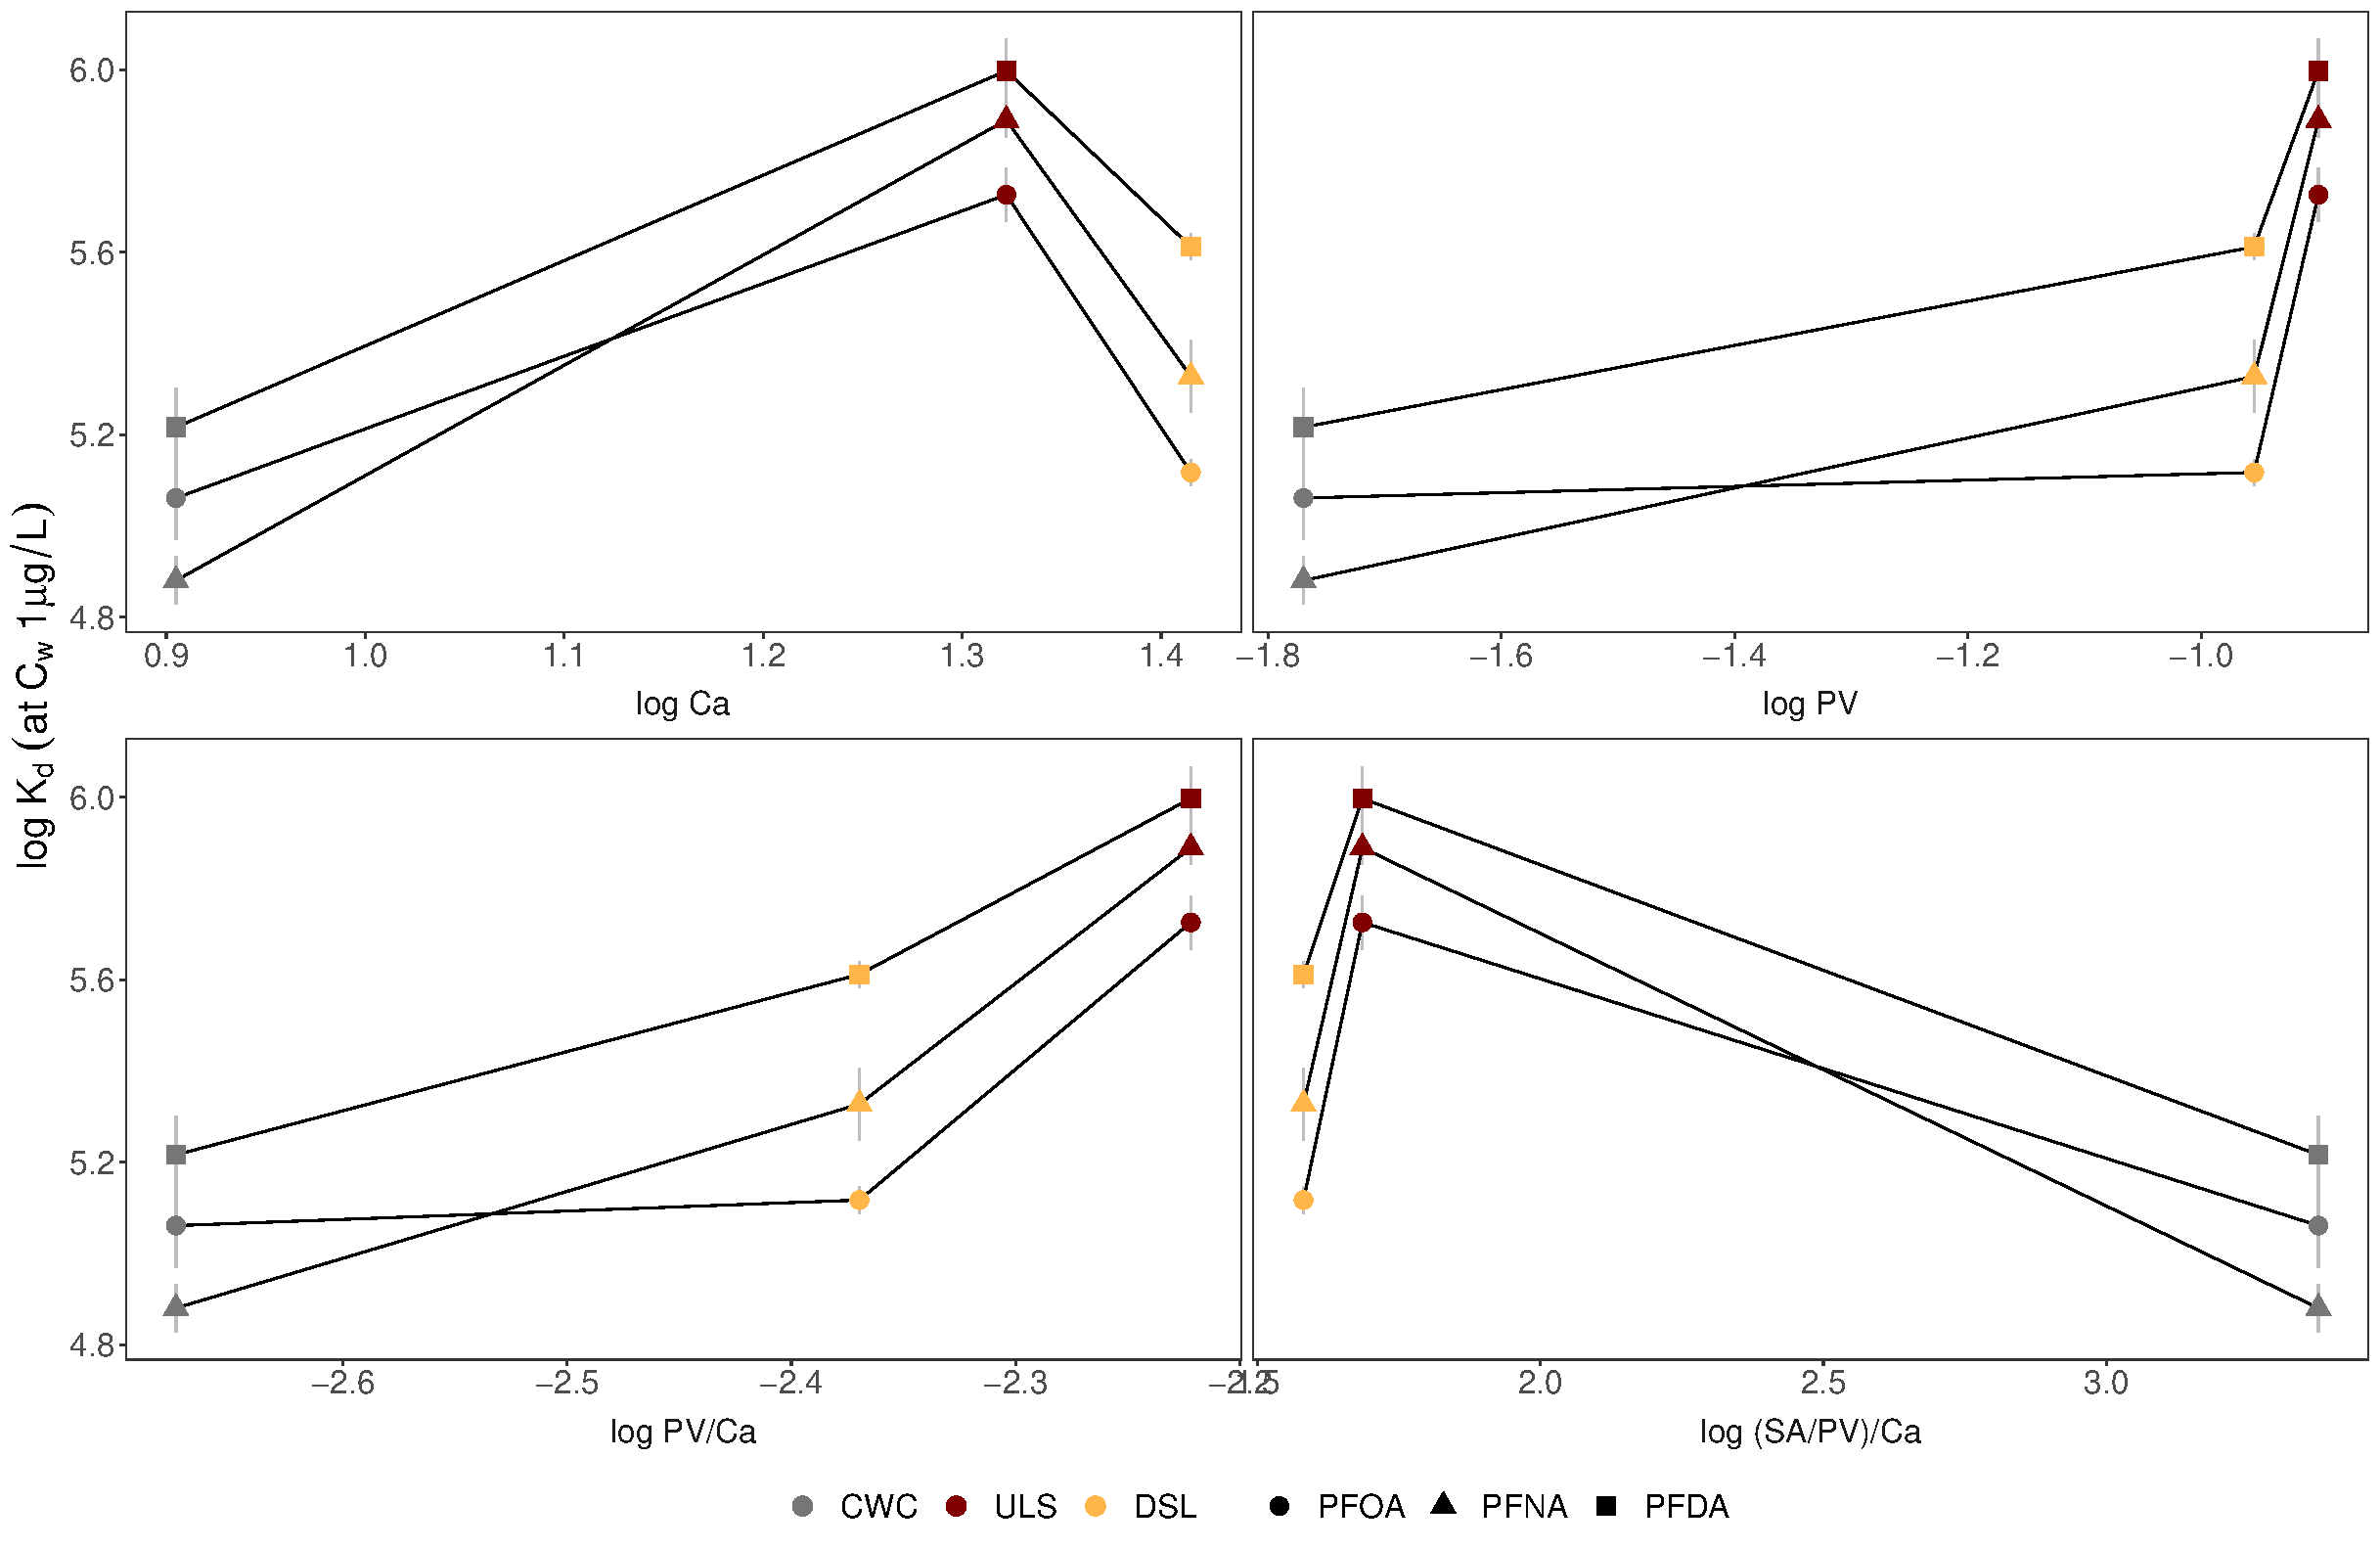
\includegraphics[width=\textwidth]{R/figs/Correlation_SAPV_Ca_plot.pdf}
    \caption{The correlation of $log~K_d$ vs. (a) log Ca (b) log PV (c) log PV/Ca (d) log (SA/PV)/Ca using BET for SA and BJH for PV by biomass feedstock. Error bars are the propagated standard error.}
    \label{fig:Kd_SAPV_Ca}
\end{figure}


Iron speciation, Synchrotron results, Inner-sphere complexes (covalent metal-ligand bonds) with Fe-carboxylate by ligand exchange \citep{gao2012adsorption}(NEED TO GET ACCESS TO ARTICLE, BUT CITED IN \citep{du2014adsorption}):

\begin{equation}
    \mathrm{\equiv Fe-OH_2^+~ + ~ CF_3(CF_2)_nCOO^- \rightarrow   ~ \equiv Fe-OOC(CF_2)_nCF_3 ~+~ H_2O}
\end{equation}




%%%%%%%%%%%%%%%%%%%%%%%%%%%%%%%%%%%%%%%%%%%%%%%%%%%%%%%%%%%%%%%%%%%%%%%%%%%%%%%%%%%%%%%%%%%%%%%%%%%%%%%%%%%%%%%%%%%%%
%%%%%%%%%%%%%%%%%%%%%%%%%%%%%%%%%%%%%%%%%%%%%%%%%%%%%%%%%%%%%%%%%%%%%%%%%%%%%%%%%%%%%%%%%%%%%%%%%%%%%%%%%%%%%%%%%%%%%
%%%%%%%%%%%%%%%%%%%%%%%%%%%%%%%%%%%%%%%%%%%%%%%%%%%%%%%%%%%%%%%%%%%%%%%%%%%%%%%%%%%%%%%%%%%%%%%%%%%%%%%%%%%%%%%%%%%%%

\section{Potential for commercializing sludge chars as sorbents}
Potential challenges with application of sewage sludge-based sorbents: leaching of heavy metals, sorption capacity, pH (although liming raises pH which is not good for sorption, addition of Ca\textsuperscript{2+} creates divalent bridging effect and complexation of PFAS molecules that enhance sorption. 

Removal efficiency, good enough for application?

Leaching of heavy metals results at PT 700 C
    As, Cd, Co, Zn, Pb for all chars Below EBC limits, Cr and Ni between lower and upper limit
    EBC = European Biochar Certificate
    Cu above EBC limits for ULS and DSL
    Enrichment factors heavy metals (?)

\subsubsection{Field conditions representativeness}

Equilibrium conditions vs laboratory batch tests
BC dose

Are the results representative of what goes on in real life? Sorption by shaking for 14 days represent an assumed equilibrium between PFCAs in the water and soil phase. A comparable situation in the field would be washing of the soil with large amounts of water such as during heavy rainfall. This will only be the case during occasional stormwater events and thus the results from this research could benefit from being supplemented with results from leaching tests using biochar mixed with soil. However, the relationship:

\begin{align}
    \frac{k_1}{k_2}
\end{align}

where \(k_1\) is the PFCA sorption (adsorption and absorption) rate and \(k_2\) is the PFCA desorption rate, where \(k_1>>k_2\), which indicates that sorption is many times higher, and in an equilibrium situation, sorption and desorption will be at steady state \citep{Cornelissen2005}. 

\section{Sustainability}
\subsection{Life cycle impact assessment (LCIA)}
LCA (life cycle assessment), sustainability aspects of production of biochar
High operating energy and cost different technologies \citep{Alhashimi2017}
Energy demand pyrolysis 

\section{Quality control of laboratory analysis and uncertainty}
Standard concentration (but at least leads to underestimation of results)
\subsection{Spiking standard concentrations}
SPE and directly, why?

The pipettes used for making the PFCA dilutions were calibrated. The three pipettes were: 1) 2-10 mL, 2) 200-1000 \textmu L, and 3) 5-50 \textmu L. All pipettes were below the permitted coefficient of variation (CV = 0.3, 0.5, and 2 $\%$ respectively (\cref{appSec:misclab}, \crefrange{appTab:pip2-10}{appTab:pip5-50}).

Since the diameter of the centrifuge tube (30 mm) was larger than that of a volumetric flask and biochar was added prior to the dilution process, the final concentration of the sorbent-sorbate mixture may have a heightened inaccuracy. However, the volume of which 0.1 g biochar occupies can be considered insignificant due to the high absorptive capacity of biochar and small mass used. Therefore a set of 10 centrifuge tubes filled to 50 mL containing 0.1 g CWC were weighed to control the uncertainty of the final dilutions. The results from weighing show that the weight of 10 trials were not accurate but precise, which means that all samples were prepared with the same final volume even though this volume deviates from 50 mL (\cref{appTab:PPcentrifuge}). 

Volume 50 mL weighed vs by eye measurement, diameter of test tube and error
preparation of cocktail standard, not consistent, some individual pipetting. 

\subsubsection{Filter blanks no significant difference}

\subsection{PFAS losses during laboratory analysis}
SPE protocol, many steps, many PP test tubes transfers, saturated PFAS-solutions, internal standard (dilutions had to disregard IS because too low concentration)

\citep{Lath2019labsorb}: 
Syringe filters: sorption of PFOA to centrifuge tubes and filter membranes. Sorption onto syringe surface: negligible due to short residence time (\textless 10 s). 74\% recovery from regenerated cellulose syringe filter. No improvement in recovery was seen when conditioning the syringe filters with phosphate solution or methanol. No trend between losses of PFOA on syringe filter and increasing spike concentrations. Centrifugation only is therefore advised if possible to avoid filtration losses. 

Test tubes: Greater recoveries from glass tubes than plastic, PP poorest recovery (55-68 \% recovery)... Contact time of PFAS residing in tubes for longer than 7 days should not be of significance, as \citep{Lath2019labsorb} propose that sorption and saturation of tube walls occur within hours. 74-81 \% recovery for PP when testing dependence on pH and ionic strength. Slight pH dependence, higher recovery at higher pH due to repulsion of negatively charged functional groups (PP has negative surface charge above pH 3.5-4. Bridging effect will be observed at higher pH's between cations like Ca2+, but is still considered negligible compared to the losses due to the physicochemical properties of the materials themselves. In general PP and plastics consists of mainly carbon hydrogen chains and are more hydrophobic than glassware. Sorption to tube walls saturate, so recoveries increase significantly with higher spike concentrations (e.g. for PP, 12-415 ug/L spiked PFOA increased recovery from 53.7-85.5 \%). Therefore, quantification of low concentrations may be subject to highest error, and in most cases will be an underestimation of dissolved concentrations. 

Use of PP test tubes, study
Higher probability of underestimating Cw for low-concentration samples because tube walls saturate – maximum number of sorption sites, there is a sorption maximum (Langmuir)

\subsection{Uncertainty}
\subsubsection{Batch tests}
Vel, du kan jo prøve å legge sammen alle de feilene. Det finnes jo forskjellige typer feilkilder i et stort forsøksoppsett. Det man ofte ser er at det er en eller to feil som er så store at de overskygger de andre. Da er det ikke noen vits å ta med alle de små. Feilen som ofte er størst er reproduserbarhet av metoden. Altså forskjellen mellom for eksempel prøver laget i triplikater. Det du kan gjøre i oppgaven din er jo å kort diskutere feilkildene du har og identifisere de største og viktigste.

\subsubsection{Analytical}
Calibration curves and matrix effect, 3-point curve
LC-MS/MS

\subsubsection{Peak integrations}
Manual review of peak integrations
decisions to remove C1 at low signal
where observed similar peak integrations across concentrations, suspected saturation of detector, dilution of these samples
\newpage

%Conclusions
\chapter{Conclusion}\label{chap:Conclusion}

Sorption increases from CWC < DSL < ULS, and with increasing perfluorinated chain-length. The Freundlich sorption coefficients (log KF) found in this study are equivalent to, or higher than, log KF  values for activated carbon reported in previous literature
Stronger sorption of PFCAs to sewage sludge biochars is likely due to a higher fraction of mesopores (2-50 nm, Fig. 5c)
A higher carbon-fraction in the pore wall matrix (lower log SA/PV/C ratio) of ULS is hypothesized to explain why PFCAs sorb stronger to ULS than to DSL 

The strong sorption of PFCAs found to sewage sludge biochars is promising for their incorporation in a circular economy, for example their use as fertilizers, sorbents in wastewater treatment plants, or as amendments to PFAS-contaminated soil
Future work should aim at further investigating the ratios between surface area, pore volume, carbon, and minerals (mainly Ca and Fe) in determining the sorption affinity of PFAS and other organic contaminants to sewage sludge biochars







\newpage

%Further work
\chapter{Recommendations for further work}\label{chap:furtherwork}

This thesis has developed a mechanistic understanding of the sorption of six PFCAs to three biochars by spiking water with known concentrations of individual PFCAs and cocktails. Future work should look more into relating this work to field-scale applications, real-life relevance. Include your idea with finding an attenuation factor for soils of increasing \%TOC to adjust the dose biochar needed to reduce PFAS pore water concentration to EQS levels. 

Multivariate regression with many chars to determine biochar properties that best contribute to sorption.

%\newpage

%Quality controls notes:

Sample matrix refers to everything present in the sample except for the target analytes. 

Reagent blank contains no sample matrix and no analytes, only labeled IS to check contamination during the extraction protocol. The reagent blank is brought through the entire extraction protocol and analyzed in the same manner as the test samples. Contamination from test tubes, reagents or other introductions of contamination will show up on the instrument results from this quality control sample. If contaminated we know that it comes from the protocol and needs to be subtracted from the rest of the samples.  % midlertidig for å se hvordan det blir. Flyttet til litterature
%\input{Konklusjon}
%input{Referanser}
% Symbolliste
%\include{Chapters/Symbolliste}
%\include{Chapters/Refferanser}
%\newpage

\bibliography{Kilder/Biochar-PFAS,Kilder/Rapporter,Kilder/History,Kilder/Jord-PFAS,Kilder/PFAS}
\addcontentsline{toc}{chapter}{Bibliography}

%\end{comment}
%%%%%%%%%%%%%%%%%%%%%%%%%%%%%%%%%%%%%%%%%%%%%%%%%%%%%%%%%%%%%%%%%%%%%%%%%%%%%%%%%%%%%%%%%%%%%%%%%%%%%%%%%%%%%%%%%%%%%%%%%%%%%%%%%%%%%%%%%%%%%%%%%%%%%%%%%%%%%%%%%%%%%%%%%%%%%%%%%%%%%%%%%%%%%%%%%%%%%%
\clearpage % for ikke ha romertall på siste side av references

%Glossary
\pagenumbering{roman}%romertall
\setcounter{page}{18}%starter sidetall på rett side, denne må oppdateres ved endelig dokument



%\addcontentsline{toc}{chapter}{Glossary}
%\input{Lister/Glossary}

% Formatering av appendix liste
%\clearpage %Brukt i artikkel
%\titleformat{\chapter}[block]{\Huge\bfseries}{Appendix \thechapter}{1em}{}
\setcounter{secnumdepth}{0}

%%  APPENDIX aka vedlegg
% Fjerner appendix figurer & tabeller fra lister https://tex.stackexchange.com/questions/213523/remove-appendix-tables-and-figures-from-list-of-figure-tables
\let\svaddcontentsline\addcontentsline
\renewcommand\addcontentsline[3]{%
  \ifthenelse{\equal{#1}{lof}}{}%
  {\ifthenelse{\equal{#1}{lot}}{}{\svaddcontentsline{#1}{#2}{#3}}}}
\appendix

% Formatering for resten av appendix
\setcounter{equation}{0}        % starter formler på 0
\setcounter{secnumdepth}{2}     % A.1, A.2 etc

\titleformat{\section}          % Kun på sections
{\normalfont\bfseries\centering} % Bold sentrert
{\thesection}                   % nummererer (A.1, A.2 etc.)
{0.5em}                         % Avstand mellom label    (nummerering) og tekst i section-tittel
{}  %https://www.overleaf.com/learn/latex/sections_and_chapters

\setlength{\headsep}{0.3cm} % avstand topptekstlinje til tekst for å få plass til mer av pdf: scale 0,85, evt justere for andre PDF størrelser

\addtocontents{toc}{\protect\setcounter{tocdepth}{0}}

% \ref{appSec:"vedleggslabel"}       gir: A,B,C...
% \ref{app:"PDFlabel"}               gir: A1, A2, B1, B2 etc.
% Merk at her brukes ikke \cref som i resten av dokumentet 

% label for hver pdf plasseres i pagecommanden etter "\section{}"
% Eks.: ..., pagecommand={\subsection{Min subsection}\label{app:OedoILs01LOG}},...

\chapter*{Appendices} % Overskrift (start på vedlegg) suppresser kapitteltall
    \phantomsection % For hyperref til funke når suppressed kapitteltall
    \addcontentsline{toc}{part}{Appendices}%
    \markboth{Appendices}{Appendices}% https://latex.org/forum/viewtopic.php?t=1309
List of appendices % Oppdater siste tall (XYZ) til siste vedleggsnummer for hvert vedlegg
\begin{itemize}
    \item \cref{appSec:ETIA}.number--number: \nameref{appSec:ETIA}
    \item \cref{appSec:IsothermSetup}. number--number: \nameref{appSec:IsothermSetup}
    \item \cref{appSec:LCMS}. number--number: \nameref{appSec:LCMS}
    \item \cref{appSec:misclab}. number--number: \nameref{appSec:misclab}
    \item \cref{appSec:elements}. number--number: \nameref{appSec:elements}
    \item \cref{appSec:pollution}. number--number: \nameref{appSec:pollution}
\end{itemize}

% Ta inn vedlegg i ønsket rekkefølge og oppdater evt listen ovenfor
\chapter{Images from ETIA unit}\label{appSec:ETIA} 

In the following section are images from the ETIA pyrolysis system at Lindum waste handling company (Drammen, Norway) presented. 


\begin{figure}
    \centering
    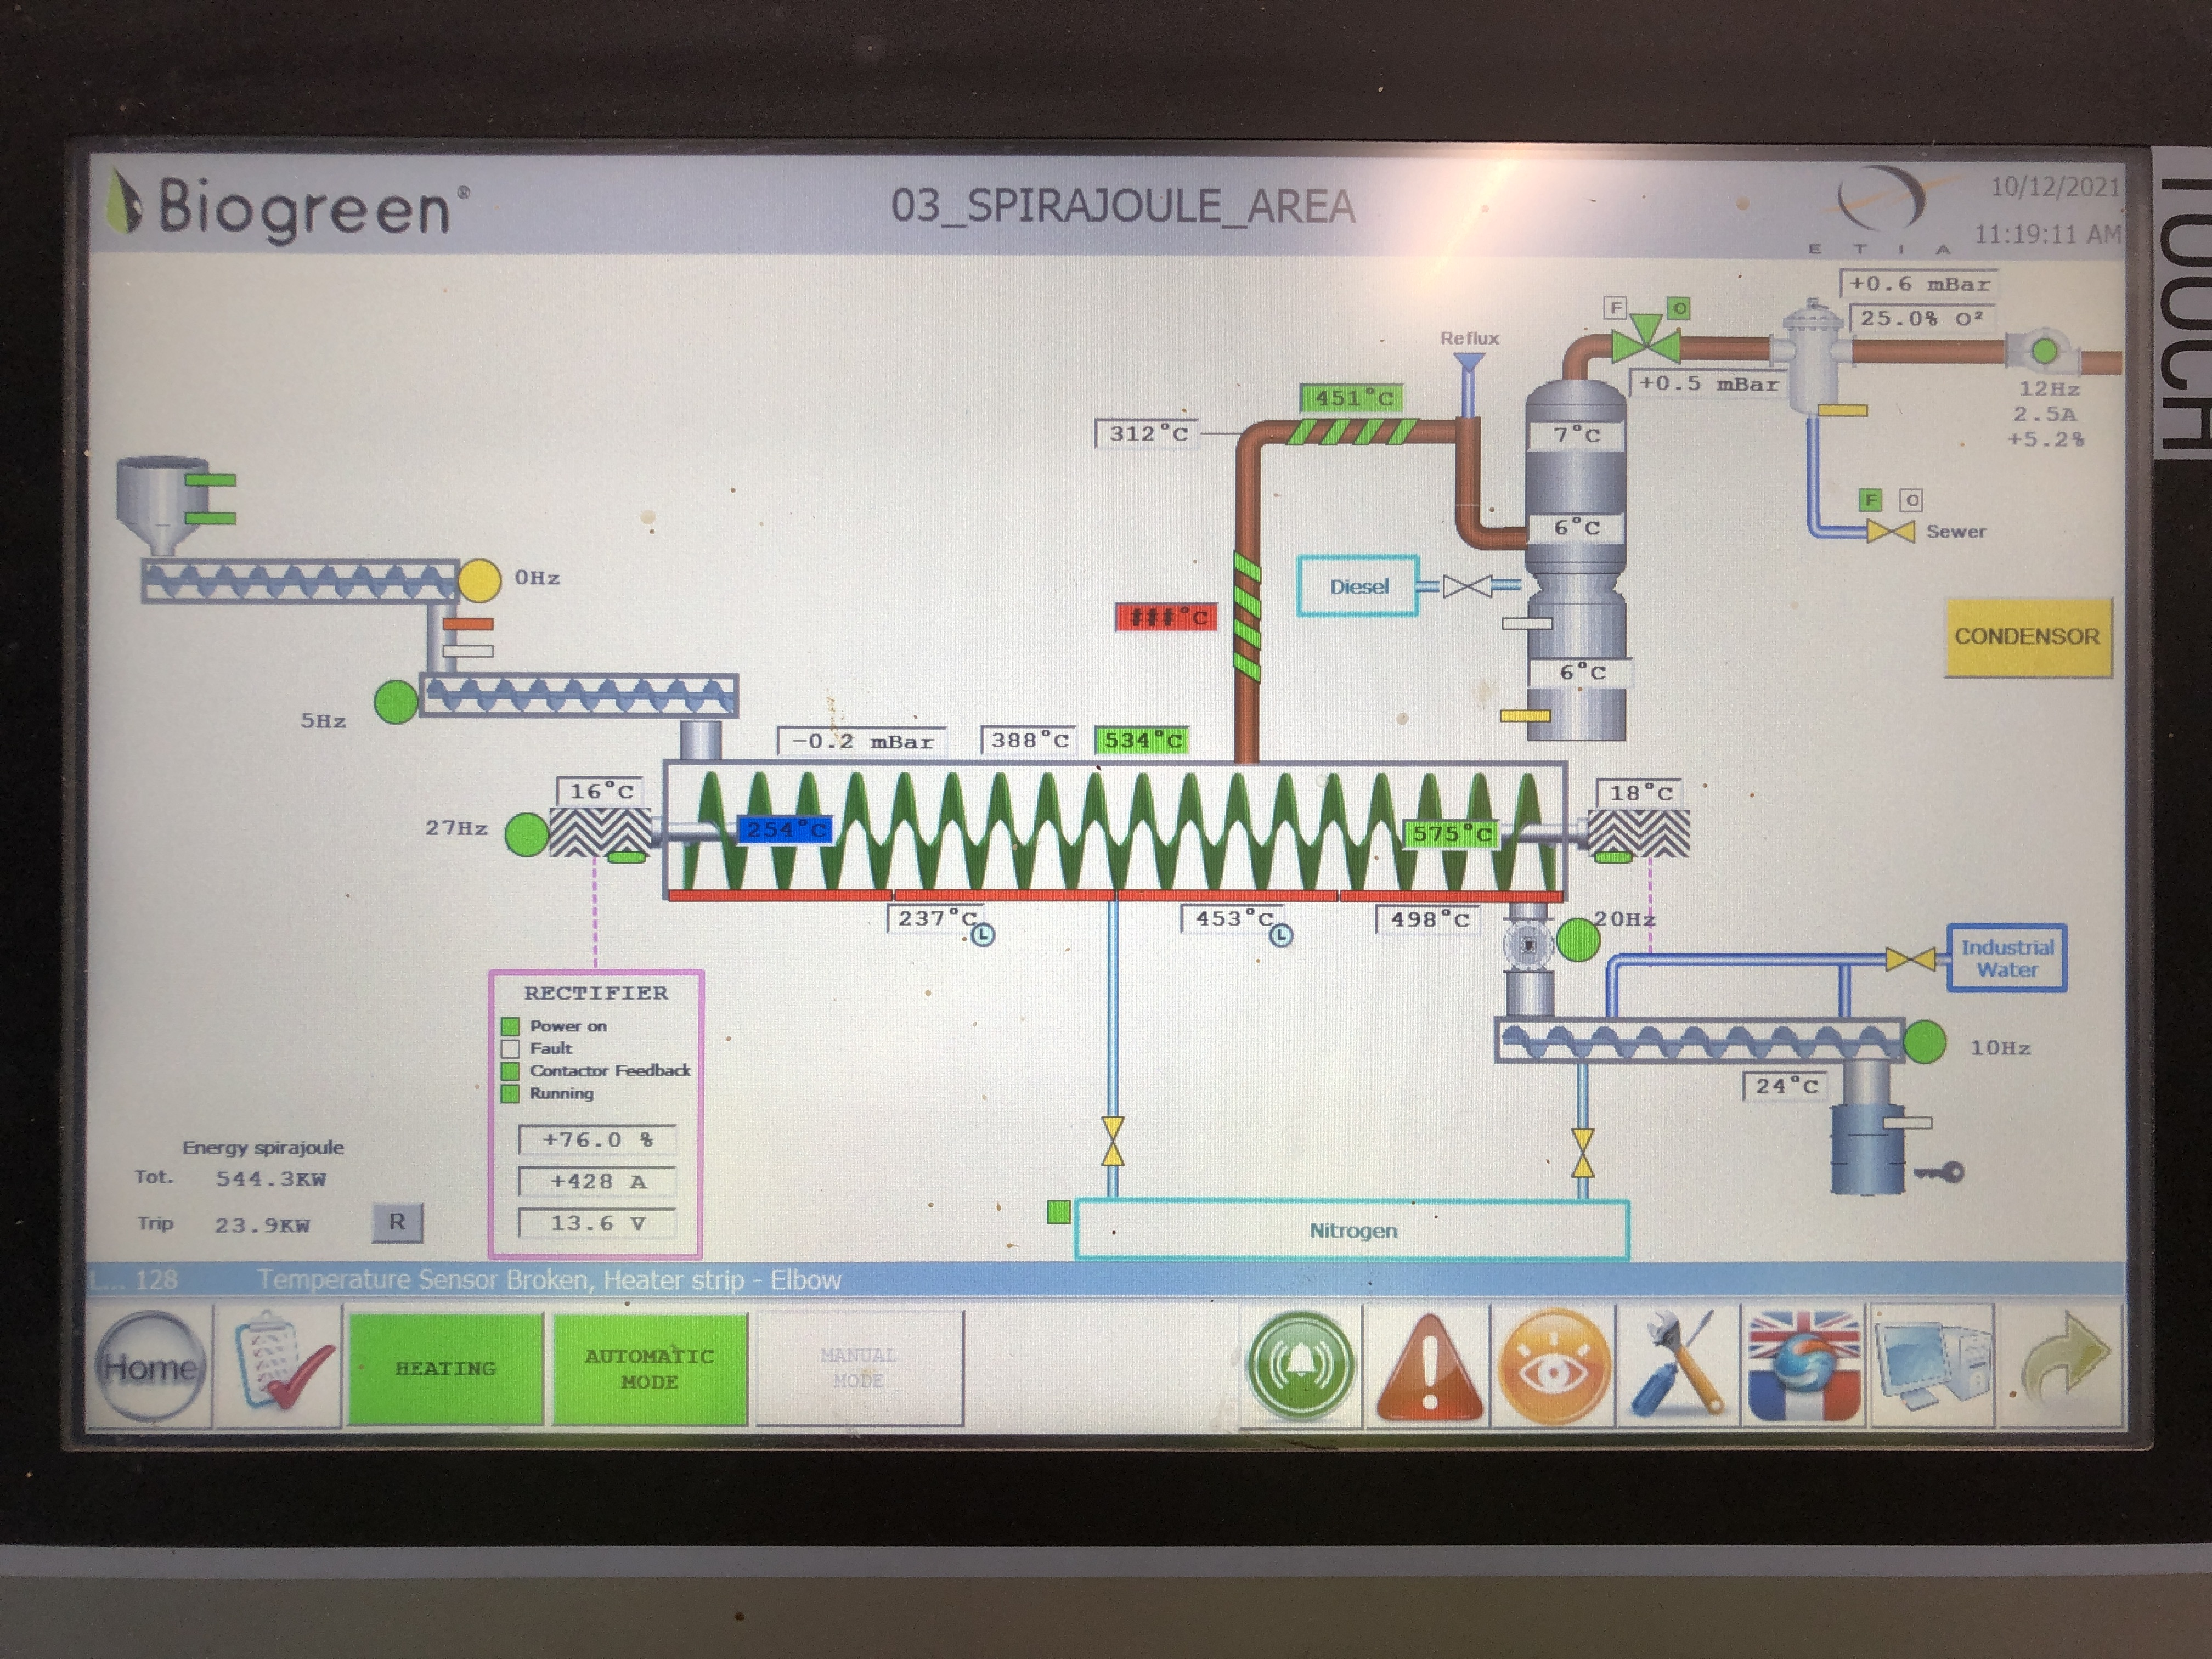
\includegraphics[width=0.7\linewidth,scale=0.7]{Bilder/Pyrolysis/Screen.png}
    \caption{Screen that displays monitoring of temperatures along the pyrolysis system developed by Biogreen\textsuperscript{\textregistered}.}
    \label{appFig:screen}
\end{figure}
\chapter{Sorption isotherm setup}\label{appSec:IsothermSetup}
In the following section, raw data for PFCA standard concentration calculations, mass of biochar weighed for each batch test, and pipetting volume are presented.

\begin{table}[h]
\centering
\caption{Concentration of first PFCA standard solution in 10 mL volumetric flasks accounted for purity of the PFCAs produced by Merck.}
\label{appTab:purityMass}
\begin{tabular}{lllll}
\toprule
Compound & Mass PFCA (g) & Purity (\%) & Mass PFCA (g) & {[}PFCA{]} (g/L) \\ 
& weighed & & accounted for purity & in   10 mL MeOH \\ \midrule
PFPeA & 0.0666 & 97 & 0.0646 & 6.46 \\
PFHxA & 0.0244 & 97 & 0.0237 & 2.37 \\
PFHpA & 0.0560 & 99 & 0.0554 & 5.54 \\
PFOA & 0.0116 & 95 & 0.0110 & 1.10 \\
PFNA & 0.0153 & 97 & 0.0148 & 1.48 \\
PFDA & 0.0114 & 98 & 0.0112 & 1.12 \\ \bottomrule
\end{tabular}
\end{table}

\begin{table}
\centering
\caption{Expected concentration of PFCA standards based on weight of native PFCA and dilution calculations versus analytical concentration by LC-MS/MS.}
\label{appTab:expConc}
\adjustbox{max width=\textwidth}{%
\begin{tabular}{lrrrrr} \toprule
 & \multicolumn{1}{l}{Me-OH standard (g L\textsuperscript{-1})} & \multicolumn{1}{l}{C11 (\textmu g L\textsuperscript{-1})} & \multicolumn{1}{l}{C12 (\textmu g L\textsuperscript{-1})} & \multicolumn{1}{l}{C13 (\textmu g L\textsuperscript{-1})} & \multicolumn{1}{l}{Analytical conc. (\textmu g L\textsuperscript{-1}}\\ \midrule
PFPeA & 6.46 & 5 168 & 103 & 15.5 & \\
PFHxA & 2.37 & 14 201 & 284 & 20.7 & \\
PFHpA & 5.60 & 3 360 & 27 & 10.2 & \\
PFOA & 1.16 & 13 920 & 557 & 13.4 & \\
PFNA & 1.53 & 18 360 & 367 & 10.0 & \\
PFDA & 1.14 & 17 100 & 684 & 10.3 & \\ \bottomrule
\end{tabular}}
\end{table}

\begin{table}
\centering
\caption{Mass biochar from Clean Wood Chips (CWC) weighed for each sample (n=60) (0.1000 $\pm$ 0.0004 g, \textmu = 0.1006 g, CV = 0.4 $\%$) C1-10 refers to the ten spike-concentrations for each PFCA batch test.}
\label{appTab:CWCmass}
\adjustbox{max width=\textwidth}{%
\begin{tabular}{lllllllllll}
\toprule
 & \multicolumn{10}{c}{Mass (g)} \\ \cline{2-11}
Compound & C1 & C2 & C3 & C4 & C5 & C6 & C7 & C8 & C9 & C10 \\ \midrule
PFPeA & 0.1008 & 0.1007 & 0.1007 & 0.1009 & 0.1014 & 0.1013 & 0.1011 & 0.1004 & 0.1009 & 0.1004 \\
PFHxA & 0.1014 & 0.1007 & 0.1014 & 0.1006 & 0.1002 & 0.1004 & 0.1014 & 0.1007 & 0.1004 & 0.1000 \\
PFHpA & 0.1005 & 0.1010 & 0.1005 & 0.1004 & 0.1009 & 0.1005 & 0.1002 & 0.1006 & 0.1007 & 0.1006 \\
PFOA & 0.1007 & 0.1008 & 0.1005 & 0.1009 & 0.1009 & 0.1002 & 0.1005 & 0.1006 & 0.1006 & 0.1009 \\
PFNA & 0.1002 & 0.1005 & 0.1004 & 0.1008 & 0.1008 & 0.1003 & 0.1002 & 0.1006 & 0.1006 & 0.1002 \\
PFDA & 0.1003 & 0.1001 & 0.1001 & 0.1001 & 0.1001 & 0.1003 & 0.1000 & 0.1005 & 0.1007 & 0.1007 \\ \bottomrule
\end{tabular}}
\end{table}


\begin{table}
\centering
\caption{Mass biochar from Ullensaker Sludge (ULS) weighed for each sample (n=60) (0.1000 $\pm$ 0.0003 g, \textmu = 0.1004 g, CV = 0.3 $\%$) C1-10 refers to the ten spike-concentrations for each PFCA batch test.}
\label{appTab:ULSmass}
\adjustbox{max width=\textwidth}{%
\begin{tabular}{lllllllllll}
\toprule
 & \multicolumn{10}{c}{Mass (g)} \\ \cline{2-11}
Compound & C1 & C2 & C3 & C4 & C5 & C6 & C7 & C8 & C9 & C10 \\ \midrule
PFPeA & 0.1007 & 0.1003 & 0.1004 & 0.1009 & 0.1009 & 0.1004 & 0.1009 & 0.1003 & 0.1000 & 0.1002 \\
PFHxA & 0.1009 & 0.1009 & 0.1003 & 0.1010 & 0.1002 & 0.1001 & 0.1006 & 0.1001 & 0.1000 & 0.1005 \\
PFHpA & 0.1001 & 0.1005 & 0.1004 & 0.1000 & 0.1004 & 0.1003 & 0.1005 & 0.1009 & 0.1005 & 0.1004 \\
PFOA & 0.1007 & 0.1000 & 0.1001 & 0.1009 & 0.1000 & 0.1001 & 0.1005 & 0.1001 & 0.1000 & 0.1002 \\
PFNA & 0.1001 & 0.1000 & 0.1000 & 0.1006 & 0.1000 & 0.1006 & 0.1005 & 0.1007 & 0.1007 & 0.1006 \\
PFDA & 0.1005 & 0.1005 & 0.1001 & 0.1008 & 0.1005 & 0.1001 & 0.1004 & 0.1002 & 0.1000 & 0.1003 \\ \bottomrule
\end{tabular}}
\end{table}

\begin{table}
\centering
\caption{Mass biochar from Biorest Lindum (BRL) weighed for each sample (n=60) (0.1000 $\pm$ 0.0003 g, \textmu = 0.1005 g, CV = 0.3 $\%$) C1-10 refers to the ten spike-concentrations for each PFCA batch test.}
\label{appTab:BRLmass}
\adjustbox{max width=\textwidth}{%
\begin{tabular}{lllllllllll}
\toprule
 & \multicolumn{10}{c}{Mass (g)} \\ \cline{2-11}
Compound & C1 & C2 & C3 & C4 & C5 & C6 & C7 & C8 & C9 & C10 \\ \midrule
PFPeA & 0.1003 & 0.1006 & 0.1000 & 0.1005 & 0.1007 & 0.1009 & 0.1005 & 0.1006 & 0.1007 & 0.1007 \\
PFHxA & 0.1003 & 0.1008 & 0.1004 & 0.0999 & 0.1004 & 0.1001 & 0.1002 & 0.1002 & 0.1007 & 0.1004 \\
PFHpA & 0.1005 & 0.1009 & 0.1010 & 0.1000 & 0.1006 & 0.1007 & 0.1007 & 0.1003 & 0.1005 & 0.1004 \\
PFOA & 0.1006 & 0.1008 & 0.1009 & 0.1002 & 0.1004 & 0.1002 & 0.1006 & 0.1001 & 0.1001 & 0.1000 \\
PFNA & 0.1010 & 0.1009 & 0.1010 & 0.1003 & 0.1002 & 0.0999 & 0.1005 & 0.1010 & 0.1005 & 0.1008 \\
PFDA & 0.1001 & 0.1007 & 0.1003 & 0.1010 & 0.1006 & 0.1008 & 0.1008 & 0.1001 & 0.1010 & 0.1004 \\ \bottomrule
\end{tabular}}
\end{table}

\begin{table}
\centering
\caption{Volume pipetted from working standards using different combinations of micro- (5-50 {\textmu}l and 200-1000 {\textmu}l) and milli pipettes (2-10 mL).}
\label{appTab:pipetting}
\adjustbox{max width=\textwidth}{%
\begin{tabular}{lrrrrrrrrrr} \toprule
\multicolumn{1}{c}{\textbf{}} & \multicolumn{10}{c}{Pipetting   volume (mL) from C11 (white) and C12 (grey)} \\ \cline{2-11} 
Compound & V1 & V2 & V3 & V4 & V5 & V6 & V7 & V8 & V9 & V10 \\ \midrule
PFPeA & \cellcolor[HTML]{C0C0C0}0.0145 & 0.314 & 0.653 & 0.967 & 1.305 & 1.620 & 1.935 & 2.274 & 2.900 & 2.902 \\
PFHxA & \cellcolor[HTML]{C0C0C0}0.0105 & 0.238 & 0.467 & 0.705 & 0.933 & 1.180 & 1.408 & 1.637 & 1.866 & 2.113 \\
PFHpA & \cellcolor[HTML]{C0C0C0}0.0240 & \cellcolor[HTML]{C0C0C0}23.250 & 0.410 & 0.632 & 0.855 & 1.079 & 1.302 & 1.525 & 1.749 & 1.935 \\
PFOA & \cellcolor[HTML]{C0C0C0}0.0110 & 0.475 & 0.960 & 1.437 & 1.922 & 2.398 & 2.874 & 3.360 & 3.843 & 4.310 \\
PFNA & \cellcolor[HTML]{C0C0C0}0.0220 & 0.483 & 0.967 & 1.457 & 1.935 & 2.425 & 2.915 & 3.390 & 3.880 & 4.357 \\
PFDA & \cellcolor[HTML]{C0C0C0}0.0365 & 1.623 & 3.245 & 4.868 & 6.490 & 8.115 & 9.737 & 11.360 & 12.982 & 14.620 \\ \bottomrule
\end{tabular}}
\end{table}

\begin{table}
\centering
\caption{Mass for each PFCA batch test prepared in 50 mL PP Falcon tubes, assuming a density of water of 1 g/mL (50.0000 $\pm$ 0.02 mL, \textmu = 50.0075 mL, CV=0.04$\%$).}
\label{appTab:milliQ}
\adjustbox{max width=\textwidth}{%
\begin{tabular}{lllllllllll} \toprule
 & \multicolumn{10}{c}{Mass (g) water weighed} \\ \cline{2-11}
Compound & V1 & V2 & V3 & V4 & V5 & V6 & V7 & V8 & V9 & V10 \\ \midrule
PFPeA & 50.0129 & 50.0108 & 50.0016 & 50.0020 & 49.9934 & 50.0001 & 50.0072 & 49.9916 & 49.9902 & 49.9943 \\
PFHxA & 50.0059 & 50.0262 & 49.9934 & 50.0107 & 50.0093 & 49.9938 & 49.9971 & 50.0015 & 50.0062 & 50.0001 \\
PFHpA & 50.0123 & 50.0084 & 50.0005 & 50.1474 & 49.9976 & 50.0055 & 49.9948 & 50.0037 & 50.0165 & 49.9950 \\
PFOA & 50.0095 & 50.0092 & 50.0128 & 49.9976 & 50.0055 & 50.0053 & 50.0036 & 50.0143 & 50.0090 & 49.9940 \\
PFNA & 50.0149 & 50.0030 & 49.9966 & 50.0463 & 50.0070 & 49.9856 & 50.0024 & 50.0062 & 50.0161 & 50.0445 \\
PFDA & 50.0120 & 50.0021 & 50.0035 & 50.0068 & 49.9963 & 50.0120 & 49.9984 & 49.9892 & 50.0101 & 50.0081 \\ \bottomrule
\end{tabular}}
\end{table}

Soil composition
\chapter{LC-MS/MS}\label{appSec:LCMS}

\begin{table}
\centering
\caption{Gradient between the two mobile phases used during UPLC-MS/MS. Water phase (A): Milli-Q water with 2 mM ammonium acetate, organic phase (B): pure MeOH. Run time = 6 min.}
\label{apptab:gradient}
\begin{tabular}{ccccc} \toprule
\multicolumn{1}{l}{\textbf{Time (min)}} & \multicolumn{1}{l}{\textbf{Flow}} & \multicolumn{1}{l}{\textbf{\% A}} & \multicolumn{1}{l}{\textbf{\% B}} & \multicolumn{1}{l}{\textbf{Step}} \\ \midrule
0 & 0.25 & 80 & 20 & Init \\
0.1 & 0.25 & 80 & 20 & 6 \\
0.2 & 0.25 & 50 & 50 & 6 \\
0.8 & 0.25 & 30 & 70 & 6 \\
1.5 & 0.25 & 20 & 80 & 6 \\
2.8 & 0.25 & 15 & 85 & 5 \\
4.5 & 0.25 & 0 & 100 & 6 \\
5.5 & 0.25 & 0 & 100 & 6 \\
5.6 & 0.25 & 80 & 20 & 6 \\
6 & 0.25 & 80 & 20 & 6 \\ \bottomrule
\end{tabular}
\end{table}

\begin{table}
\centering
\caption{Tune parameters for UPLC-Xevo TQS instrument.}
\label{apptab:tune}
\begin{tabular}{ll} \toprule
\multicolumn{1}{c}{\textbf{ESI (-)}} &  \\ \midrule
Capillary (kV) & 2 \\
Cone (V) & 25 \\
Source Offset (V) & 40 \\
Desolvation temperature   (\textdegree C) & 450 \\
Desolvation Gas flow   (L/h) & 650 \\
Cone (L/h) & 150 \\
Nebuliszer (Bar) & 6 \\
Source Temperature (\textdegree C) & 150 \\ \bottomrule
\end{tabular}
\end{table}

\begin{figure}
    \centering
    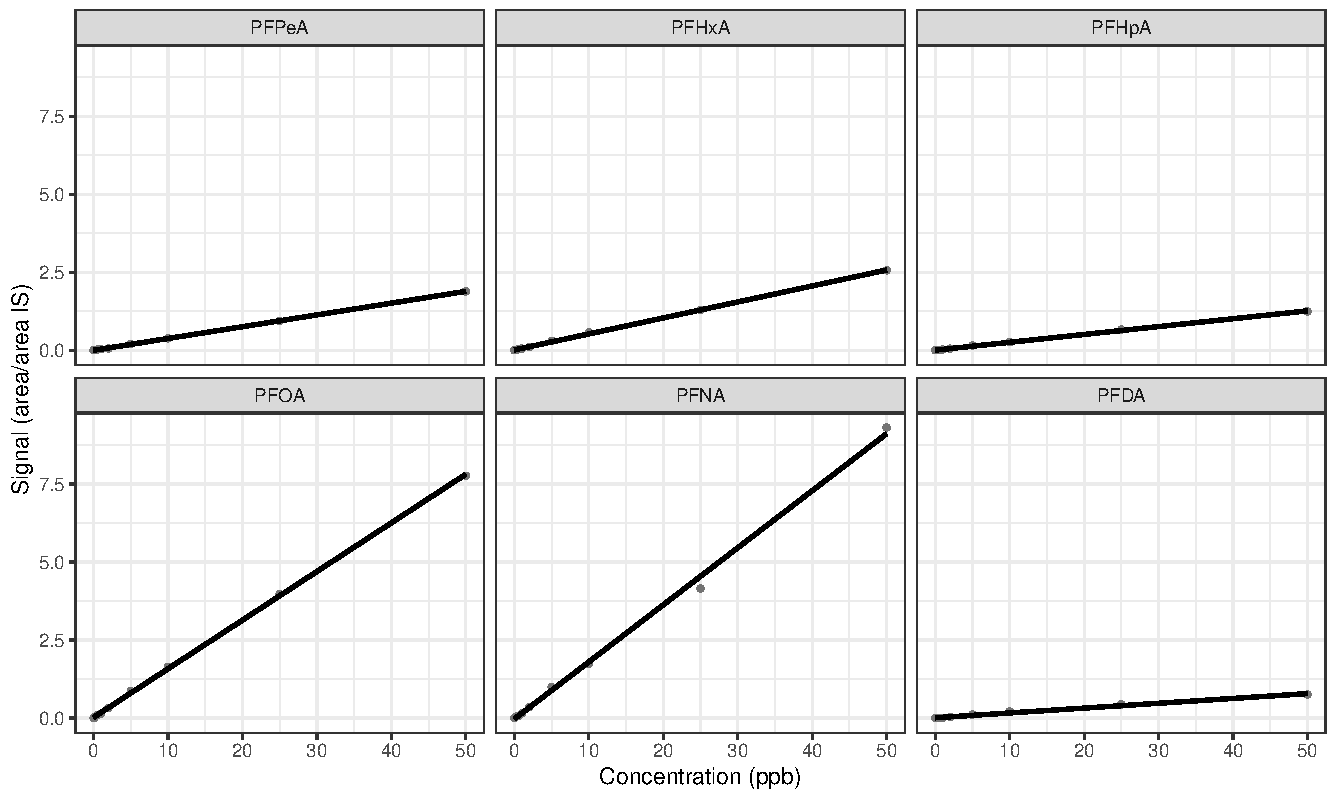
\includegraphics[width=\textwidth]{R/figs/CC_all.pdf}
    \caption{Calibration curve solvent blank}
    \label{appfig:CC}
\end{figure}

Matrix effect

\begin{figure}
    \centering
    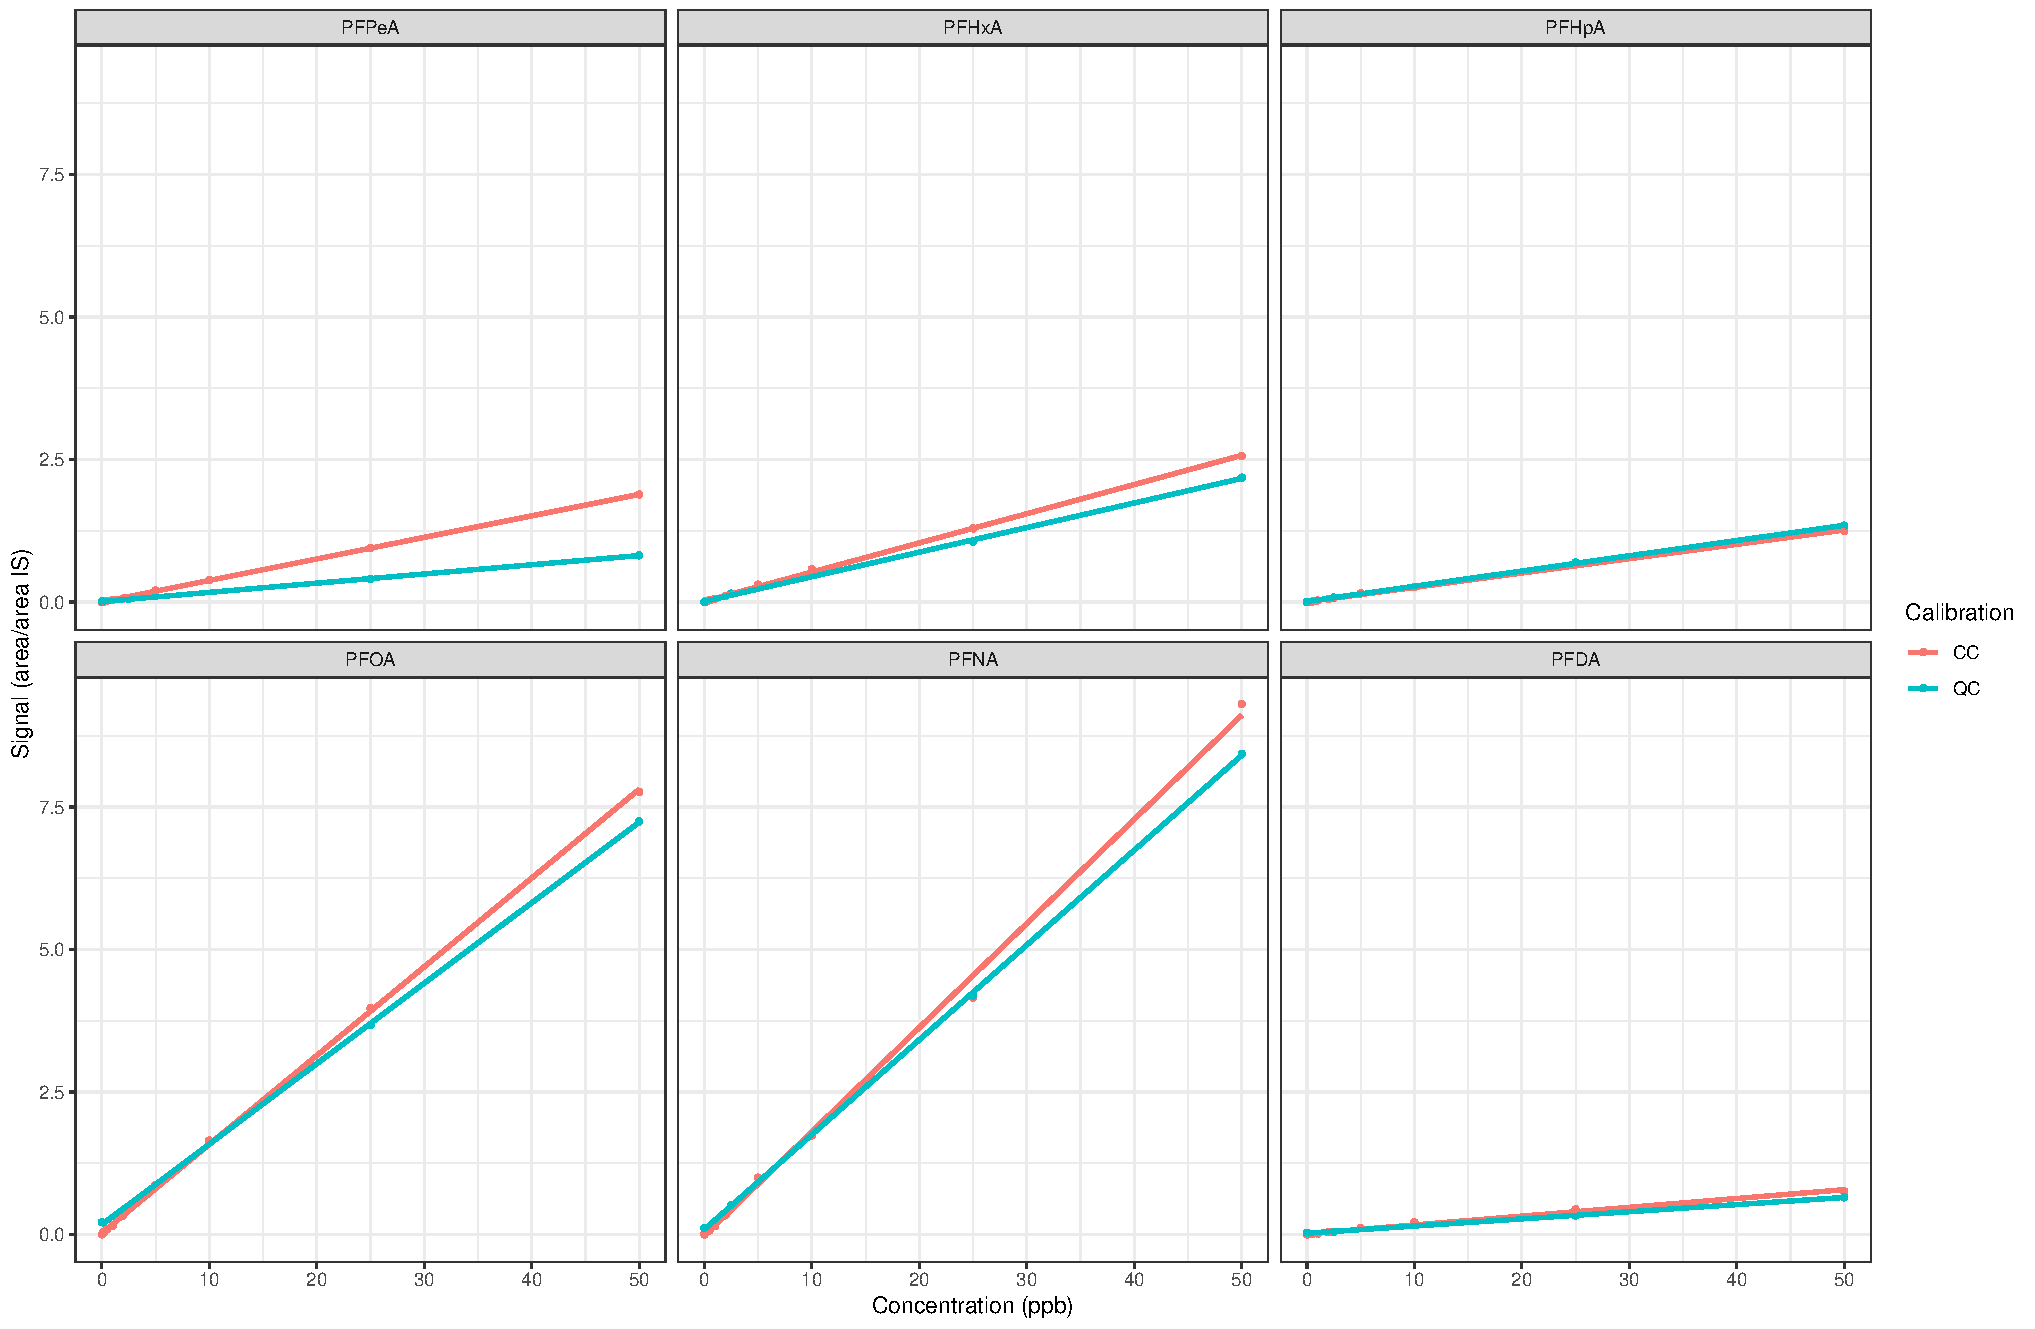
\includegraphics[width=\textwidth]{R/figs/CCQC_matrixeffect.pdf}
    \caption{Matrix effect (ME) for the PFCAs where CC = calibration curve in solvent blank, QC = matrix matched calibration curve. QC in line with CC indicates no ME, QC \textgreater CC = ion enhancement, CC \textless QC = ion suppression.}
    \label{appfig:ME}
\end{figure}
\chapter{Miscellaneous laboratory tests}\label{appSec:misclab}

In the following section, miscellaneous laboratory performed to strengthen the experimental certainty of the batch sorption isotherm tests are presented. 

\subsection{pH and conductivity}

\begin{figure} 
\centering
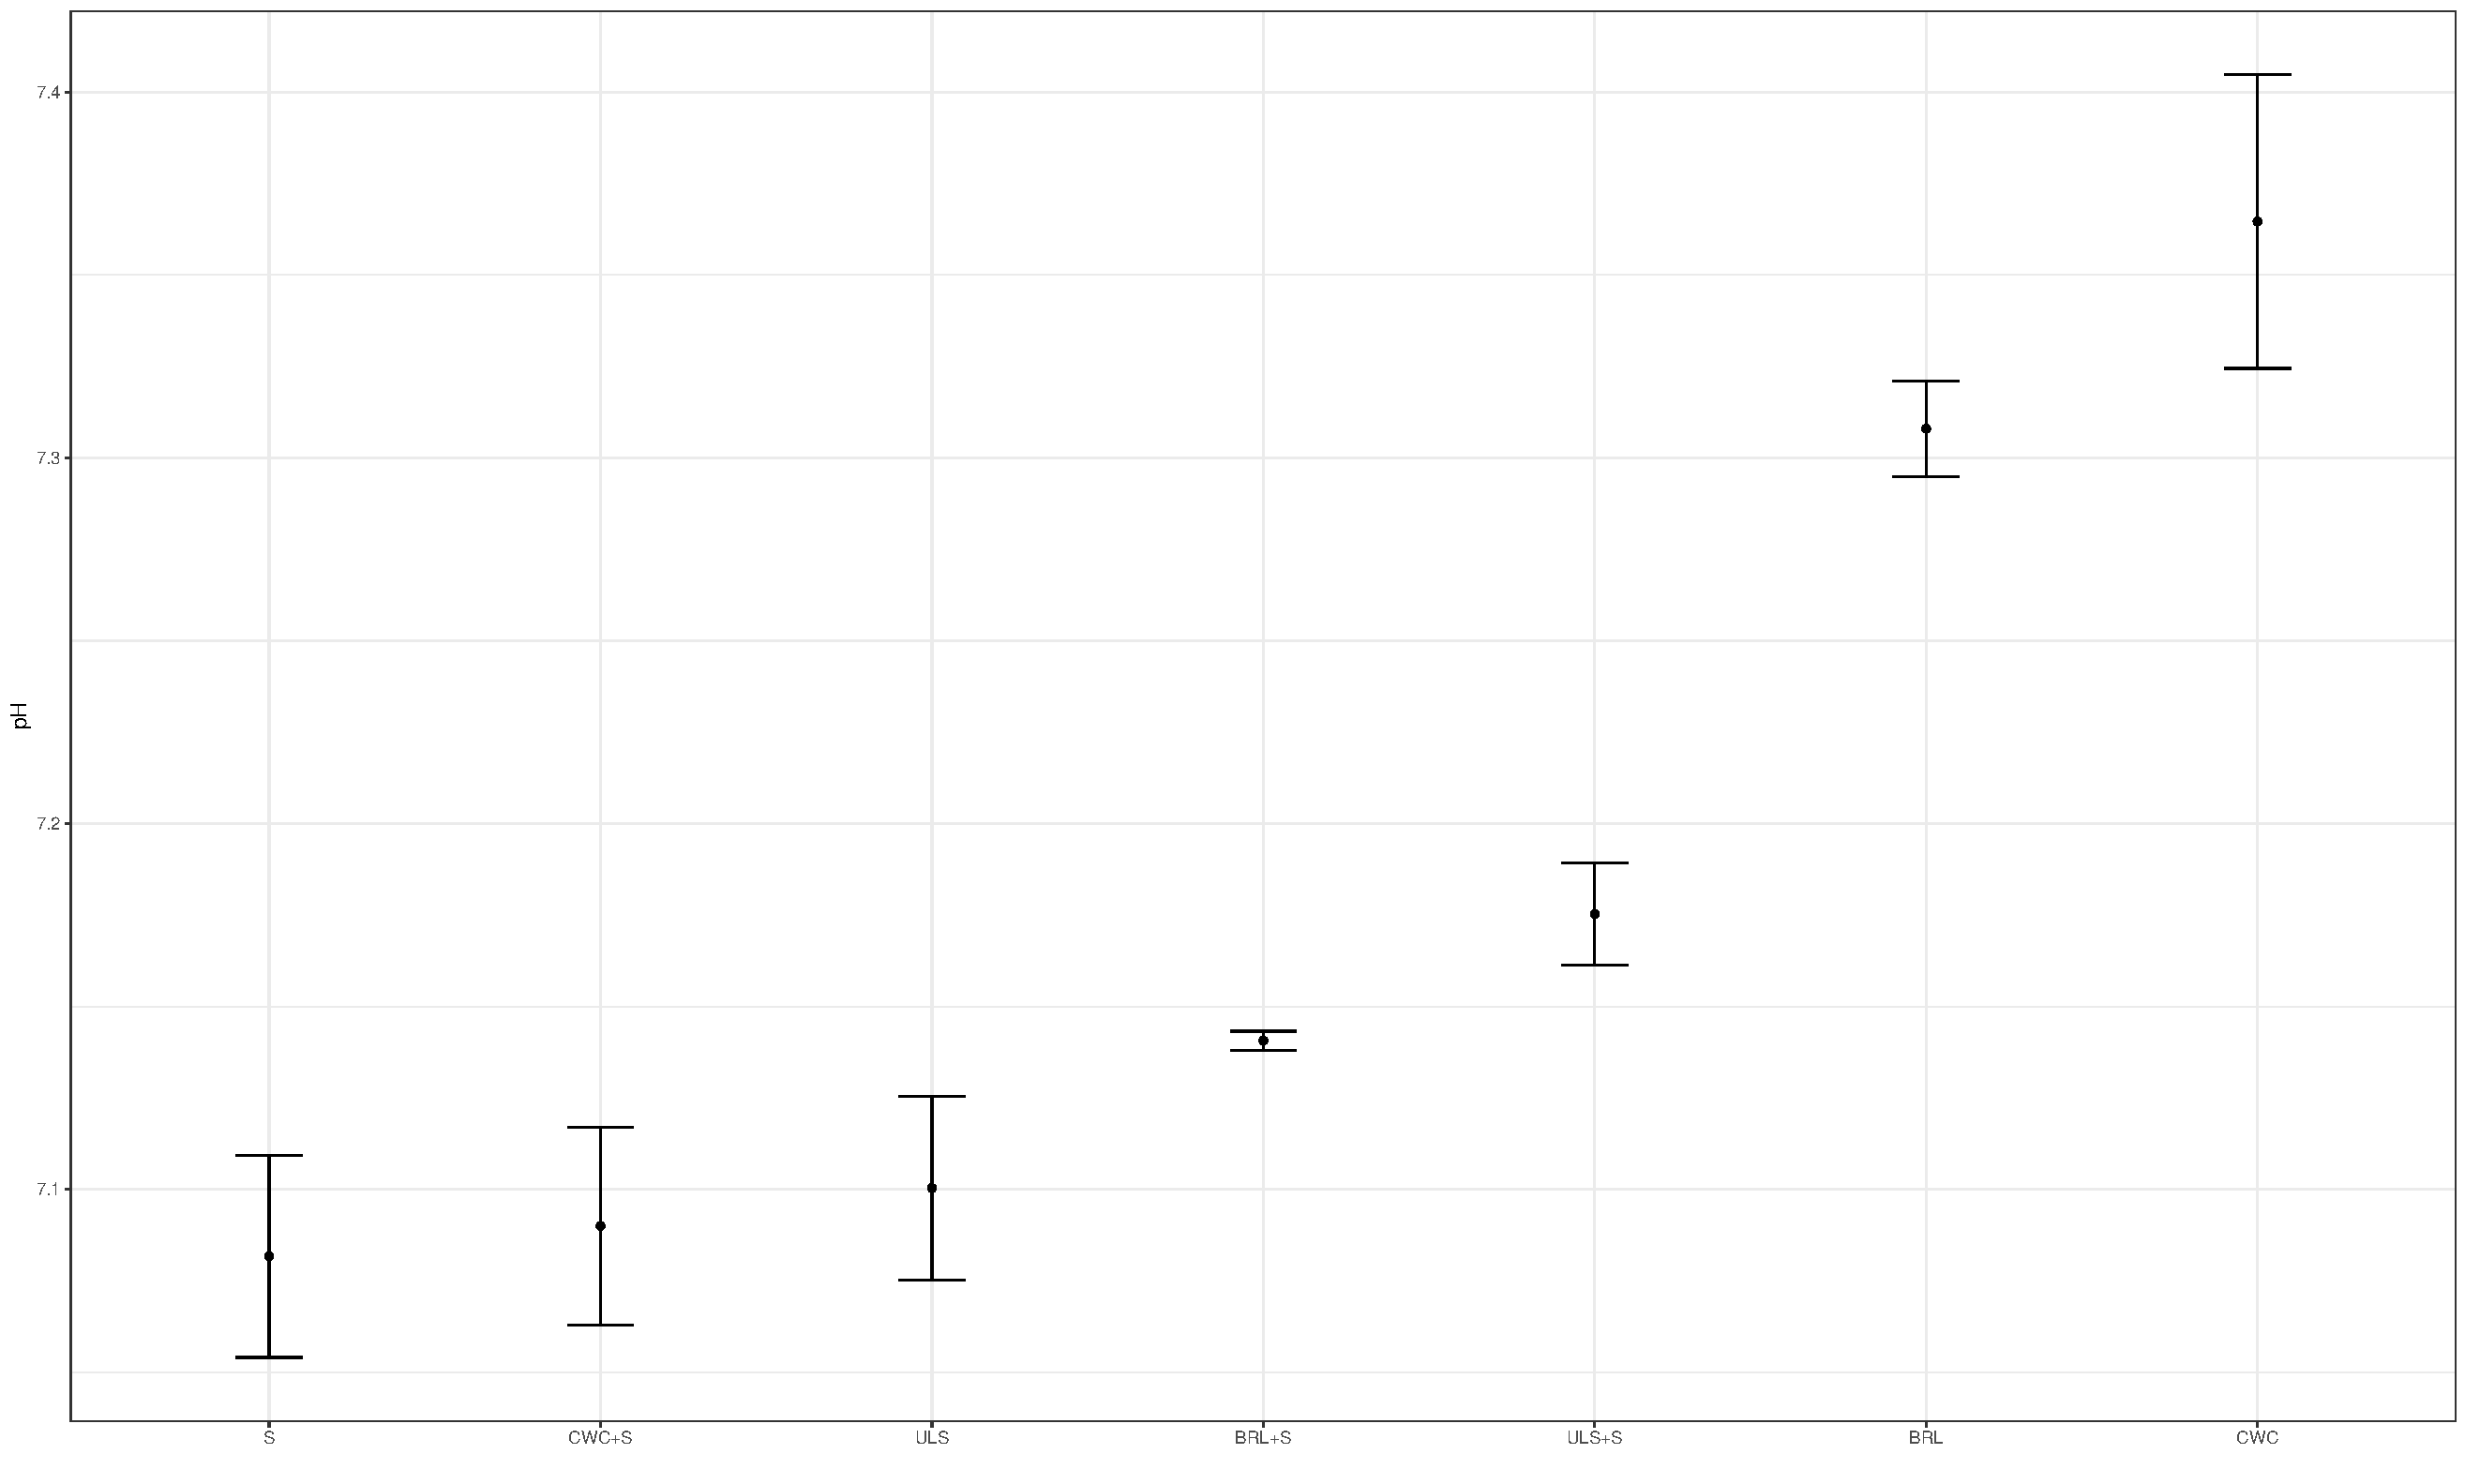
\includegraphics[width=\textwidth]{R/figs/pH.pdf}
\caption{Plot of pH measurements for 50 mL milli-Q water batch tests with 0.1 g biochars (CWC, ULS, BRL) and 5 g soil (S) (n=3).}
\label{appfig:pH}
\end{figure}

\begin{figure} 
\centering
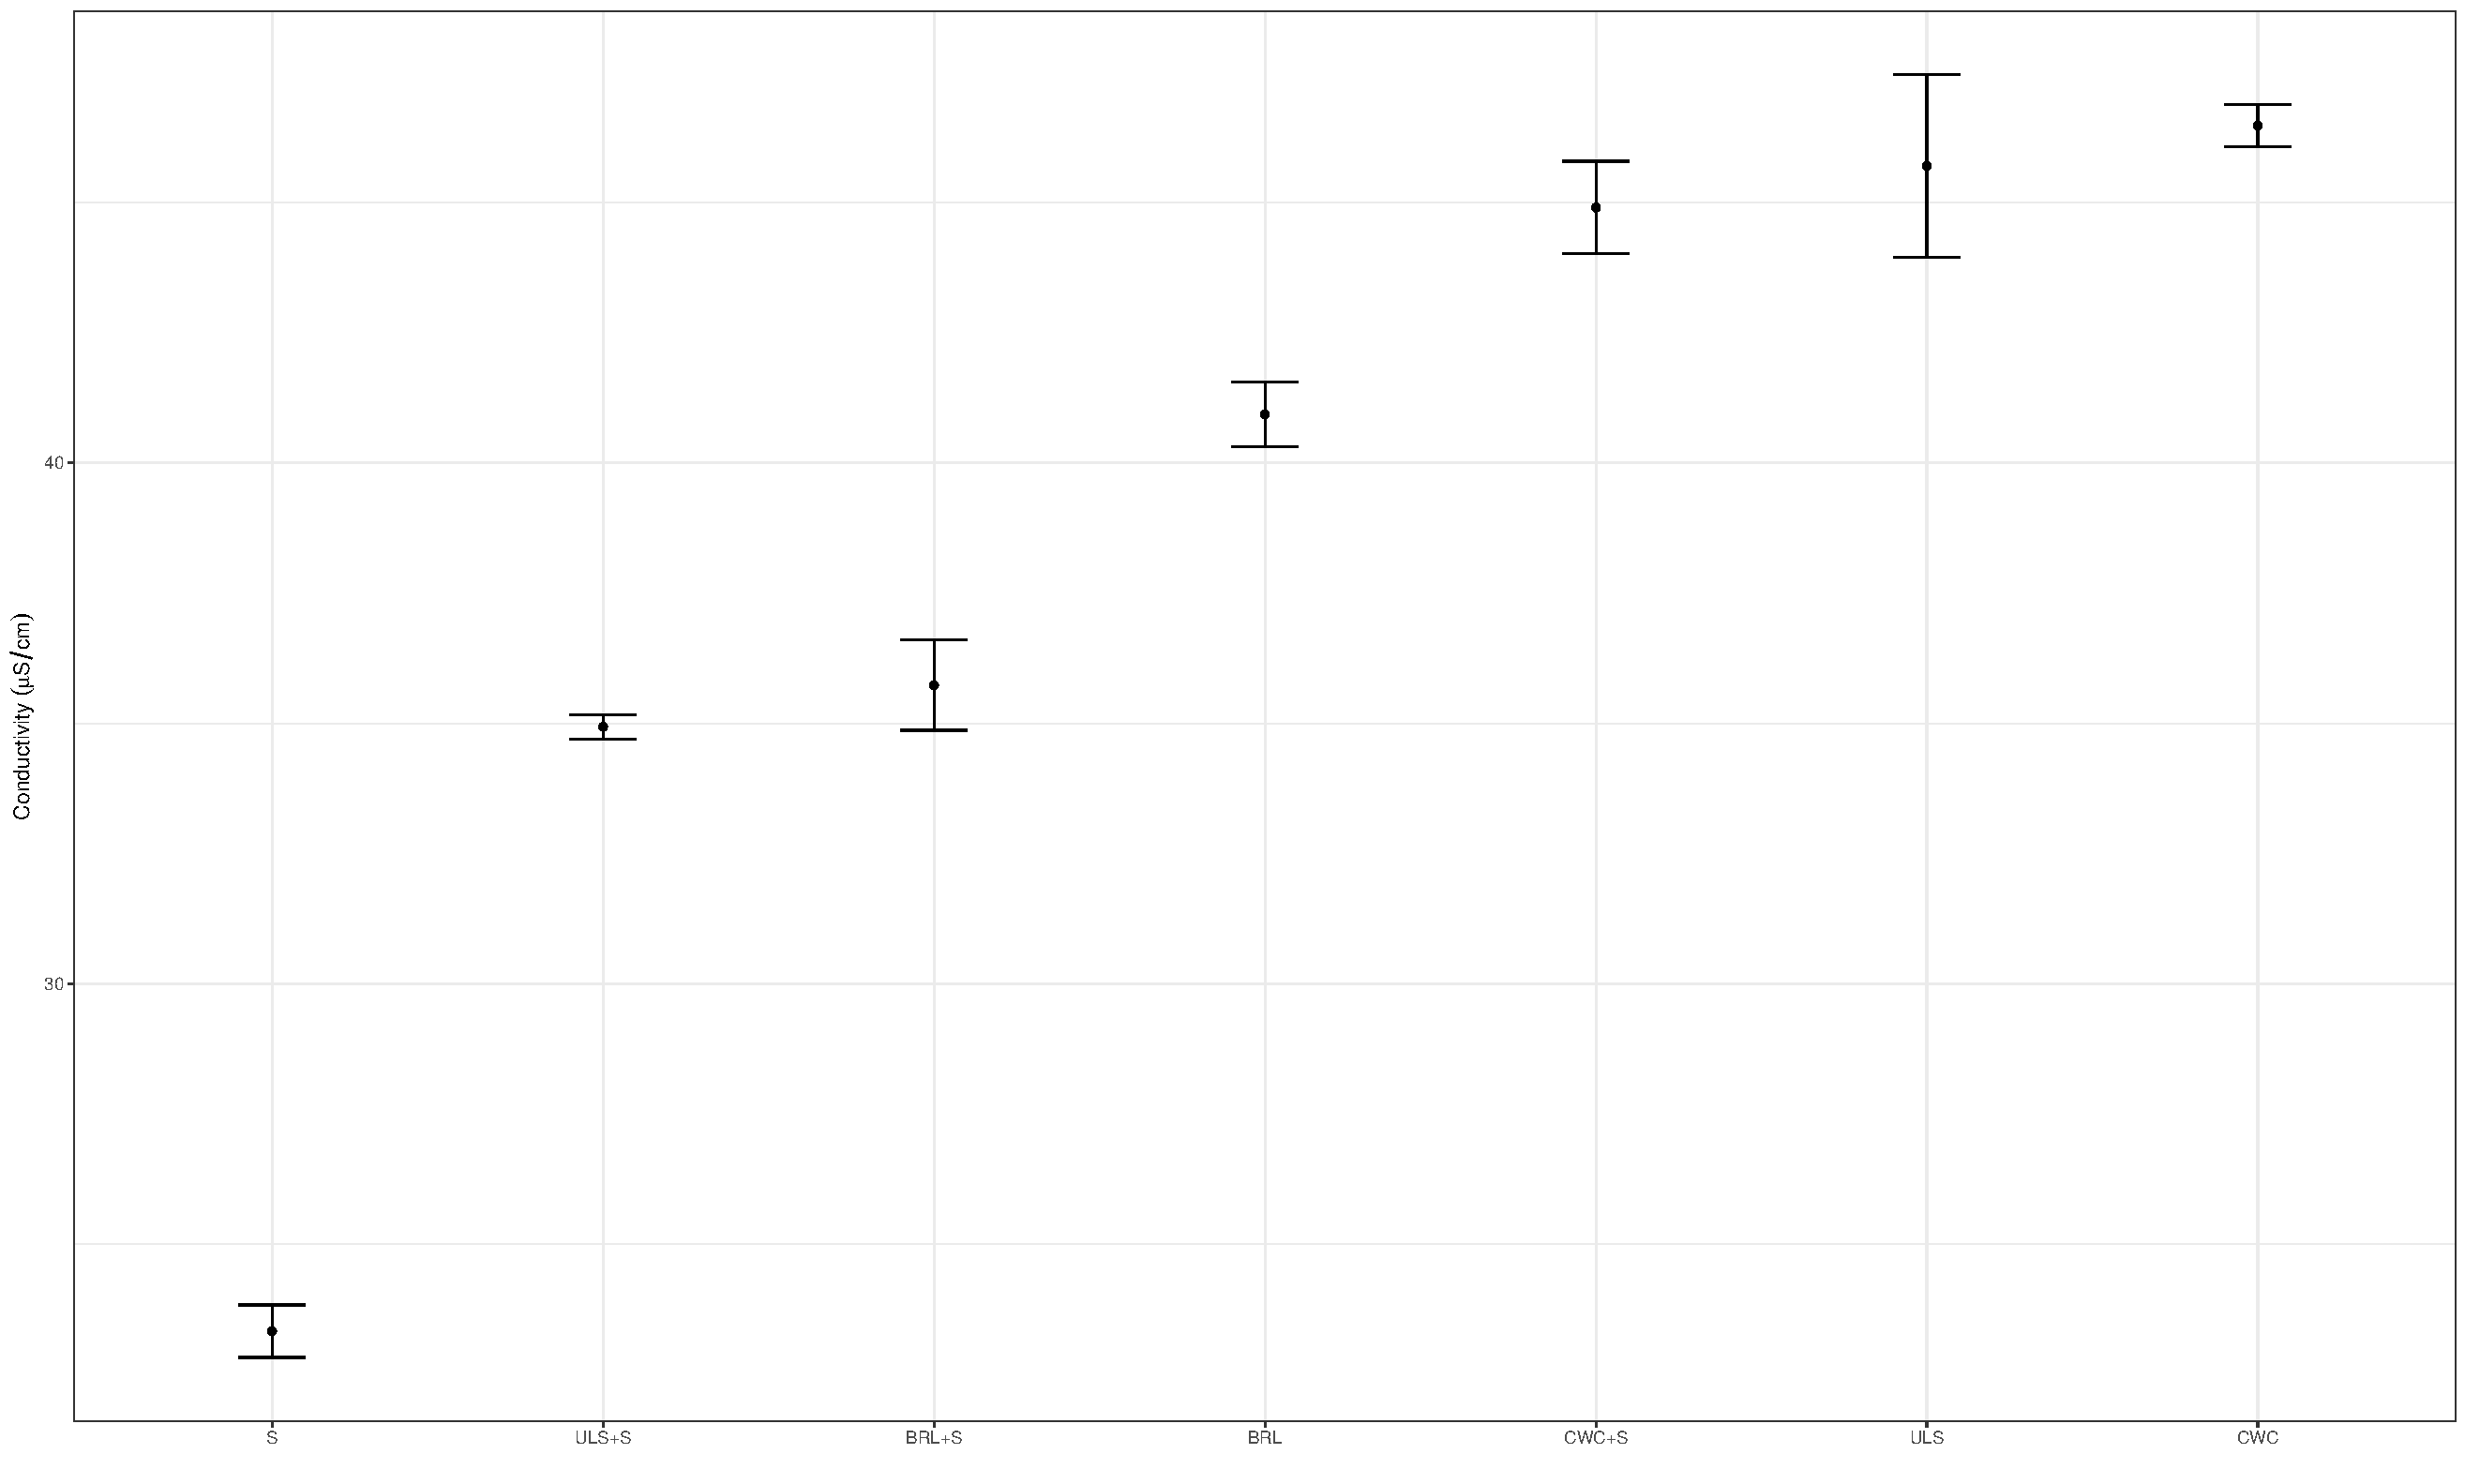
\includegraphics[width=\textwidth]{R/figs/conductivity.pdf}
\caption{Plot of conductivity measurements for 50 mL milli-Q water batch tests with 0.1 g biochars (CWC, ULS, BRL) and 5 g soil (S) (n=3).}
\label{appfig:cond}
\end{figure}

\begin{table}[h]
\centering
\caption{Pipette calibration for 2-10 mL pipette. PASS is given if CV $\leq$ 1.0 \% and the average volume dispensed is within 1.8400 - 2.1600 mL. }
\label{appTab:pip2-10}
\adjustbox{max width=\textwidth}{%
\begin{tabular}{lrrrrrrr} \toprule
 & \multicolumn{1}{l}{} &  &  &  & \multicolumn{3}{r}{Operator: Thermo Fishcer Scientific} \\
 & \multicolumn{1}{l}{} &  &  &  & \multicolumn{3}{r}{Serial number: EJ08813} \\
 & \multicolumn{1}{l}{} &  &  &  & \multicolumn{3}{r}{Date: 04.10.2021} \\ \midrule
\multicolumn{1}{c}{\textbf{\begin{tabular}[c]{@{}c@{}}Test volume\\ (mL)\end{tabular}}} & \multicolumn{1}{c}{\textbf{}} & \multicolumn{1}{c}{\textbf{\begin{tabular}[c]{@{}c@{}}Weight of\\ dispensed\\ volume (g)\end{tabular}}} & \multicolumn{1}{c}{\textbf{\begin{tabular}[c]{@{}c@{}}Corrected\\ volume (g)\end{tabular}}} & \multicolumn{1}{c}{\textbf{\begin{tabular}[c]{@{}c@{}}Average\\ volume (mL)\end{tabular}}} & \multicolumn{1}{c}{\textbf{SDEV}} & \multicolumn{1}{c}{\textbf{CV}} & \multicolumn{1}{c}{\textbf{PASS/FAIL}} \\ \midrule
\multicolumn{1}{c}{\textbf{2}} & \multicolumn{1}{c}{\textbf{}} &  &  & 2.0868 & 0.006 & 0.3 \% &  \\
\multicolumn{1}{c}{\textbf{}} & 1 & 2.0804 & 2.0842 &  &  &  &  \\
 & 2 & 2.0923 & 2.0961 &  &  &  &  \\
 & 3 & 2.0902 & 2.0940 &  &  &  &  \\
 & 4 & 2.0861 & 2.0899 &  &  &  &  \\
 & 5 & 2.0817 & 2.0855 &  &  &  &  \\
 & 6 & 2.0852 & 2.0890 &  &  &  &  \\
 & 7 & 2.0807 & 2.0845 &  &  &  &  \\
 & 8 & 2.0829 & 2.0867 &  &  &  &  \\
 & 9 & 2.0778 & 2.0815 &  &  &  & \textbf{} \\
 & 10 & 2.0727 & 2.0764 &  &  &  &  \\
 & \multicolumn{1}{l}{} &  &  & \textbf{} & \textbf{} &  & \cellcolor[HTML]{C0C0C0}\textbf{PASS} \\ \bottomrule
\end{tabular}}
\end{table}



\begin{table}
\centering
\caption{Pipette calibration for 200-1000 μL pipette. PASS is given if CV $\leq$ 1.0 \% and the average volume dispensed is within 992 - 1008 μL. }
\label{appTab:pip200-1000}
\adjustbox{max width=\textwidth}{%
\begin{tabular}{lrrrrrrr} \toprule
 & \multicolumn{1}{l}{} & \multicolumn{1}{l}{} & \multicolumn{1}{l}{} & \multicolumn{1}{l}{} & \multicolumn{3}{r}{Operator: Thermo Fischer Scientific} \\
 & \multicolumn{1}{l}{} & \multicolumn{1}{l}{} & \multicolumn{1}{l}{} & \multicolumn{1}{l}{} & \multicolumn{3}{r}{Serial Number: EH23798 4500} \\
 & \multicolumn{1}{l}{} & \multicolumn{1}{l}{} & \multicolumn{1}{l}{} & \multicolumn{1}{l}{} & \multicolumn{3}{r}{Date: 04.10.2021} \\ \midrule
\multicolumn{1}{c}{\textbf{\begin{tabular}[c]{@{}c@{}}Test volume \\ (μL)\end{tabular}}} & \textbf{} & \multicolumn{1}{c}{\textbf{\begin{tabular}[c]{@{}c@{}}Weight of\\ dispensed\\ volume (g)\end{tabular}}} & \multicolumn{1}{c}{\textbf{\begin{tabular}[c]{@{}c@{}}Corrected\\ volume (μL)\end{tabular}}} & \multicolumn{1}{c}{\textbf{\begin{tabular}[c]{@{}c@{}}Average\\ volume (μL)\end{tabular}}} & \multicolumn{1}{c}{\textbf{SDEV}} & \multicolumn{1}{c}{\textbf{CV}} & \multicolumn{1}{c}{\textbf{PASS/FAIL}} \\ \midrule
\multicolumn{1}{c}{\textbf{1000}} & \textbf{} & \multicolumn{1}{l}{} & \multicolumn{1}{l}{} & 994.2 & 5 & 0.5 \% & \multicolumn{1}{l}{} \\
\multicolumn{1}{c}{} & 1 & 997.0 & 998.8 &  &  &  &  \\
 & 2 & 999.4 & 1001.2 &  &  &  &  \\
 & 3 & 990.4 & 992.2 &  &  &  &  \\
 & 4 & 992.3 & 994.1 &  &  &  &  \\
 & 5 & 990.5 & 992.3 &  &  &  &  \\
 & 6 & 990.9 & 992.7 &  &  &  &  \\
 & 7 & 983.8 & 985.6 &  &  &  &  \\
 & 8 & 990.9 & 992.7 &  &  &  &  \\
 & 9 & 990.5 & 992.3 &  &  &  &  \\
 & 10 & 998.4 & 1000.2 &  &  &  &  \\
 & \multicolumn{1}{l}{} & \multicolumn{1}{l}{} & \multicolumn{1}{l}{} & \multicolumn{1}{l}{\textbf{}} & \multicolumn{1}{l}{\textbf{}} & \multicolumn{1}{l}{} & \multicolumn{1}{l}{\cellcolor[HTML]{C0C0C0}\textbf{PASS}} \\ \bottomrule
\end{tabular}}
\end{table}


\begin{table}
\centering
\caption{Pipette calibration for 5 - 50 μL pipette. PASS is given if CV $\leq$ 2.5 \% and the average volume dispensed is within 19.8 - 20.2 μL. }
\label{appTab:pip5-50}
\adjustbox{max width=\textwidth}{%
\begin{tabular}{lrrrrrrr} \toprule
 & \multicolumn{1}{l}{} & \multicolumn{1}{l}{} & \multicolumn{1}{l}{} & \multicolumn{1}{l}{} & \multicolumn{3}{r}{Operator: Thermo Fischer Scientific} \\
 & \multicolumn{1}{l}{} & \multicolumn{1}{l}{} & \multicolumn{1}{l}{} & \multicolumn{1}{l}{} & \multicolumn{3}{r}{Serial Number: EH94947 4500} \\
 & \multicolumn{1}{l}{} & \multicolumn{1}{l}{} & \multicolumn{1}{l}{} & \multicolumn{1}{l}{} & \multicolumn{3}{r}{Date: 04.10.2021} \\ \midrule
\multicolumn{1}{c}{\textbf{\begin{tabular}[c]{@{}c@{}}Test volume\\ (μL)\end{tabular}}} & \multicolumn{1}{c}{\textbf{}} & \multicolumn{1}{c}{\textbf{\begin{tabular}[c]{@{}c@{}}Weight of\\ dispensed\\ volume (g)\end{tabular}}} & \multicolumn{1}{c}{\textbf{\begin{tabular}[c]{@{}c@{}}Corrected\\ volume (mL)\end{tabular}}} & \multicolumn{1}{c}{\textbf{\begin{tabular}[c]{@{}c@{}}Average\\ volume (mL)\end{tabular}}} & \multicolumn{1}{c}{\textbf{SDEV}} & \multicolumn{1}{c}{\textbf{CV}} & \multicolumn{1}{c}{\textbf{PASS/FAIL}} \\ \midrule
\multicolumn{1}{c}{\textbf{20}} & &  &  & 19.8 & 0.4 & 2 $\%$ & \multicolumn{1}{l}{} \\
 & 1 & 19.8 & 19.8 &  &  &  &  \\
 & 2 & 19.5 & 19.5 &  &  &  &  \\
 & 3 & 19.8 & 19.8 &  &  &  &  \\
 & 4 & 20.8 & 20.8 &  &  &  &  \\
 & 5 & 19.9 & 19.9 &  &  &  &  \\
 & 6 & 19.6 & 19.6 &  &  &  &  \\
 & 7 & 19.7 & 19.7 &  &  &  &  \\
 & 8 & 19.5 & 19.5 &  &  &  &  \\
 & 9 & 19.2 & 19.2 &  &  &  &  \\
 & 10 & 19.9 & 19.9 &  &  &  & \cellcolor[HTML]{FFFFFF}\textbf{} \\
 & \multicolumn{1}{l}{} & \multicolumn{1}{l}{} & \multicolumn{1}{l}{} &  &  &  & \multicolumn{1}{l}{\cellcolor[HTML]{C0C0C0}\textbf{PASS}} \\ \bottomrule
\end{tabular}}
\end{table}

\begin{table}
\centering
\caption{Volume calibration for 50 mL Falcon high-clarity polypropylene (PP) conical centrifuge tube. PASS is given if CV $\leq$ and the average volume filled is within 49.0 - 51.0 mL.}
\label{appTab:PPcentrifuge}
\adjustbox{max width=\textwidth}{%
\begin{tabular}{crrrrrrrr} \toprule
 &  &  &  &  & \multicolumn{4}{r}{Date: 26.10.2021} \\ \midrule
\multicolumn{1}{c}{\textbf{\begin{tabular}[c]{@{}c@{}}Test\\volume (mL)\end{tabular}}} & \multicolumn{1}{c}{\textbf{}} & \multicolumn{1}{c}{\textbf{\begin{tabular}[c]{@{}c@{}}Initial \\ weight  (g)\end{tabular}}} & \multicolumn{1}{c}{\textbf{\begin{tabular}[c]{@{}c@{}}Final\\weight (g)\end{tabular}}} & \multicolumn{1}{c}{\textbf{\begin{tabular}[c]{@{}c@{}}Net \\weight (g)\end{tabular}}} & \multicolumn{1}{c}{\textbf{\begin{tabular}[c]{@{}c@{}}Average \\ volume (mL)\end{tabular}}} & \multicolumn{1}{c}{\textbf{SDEV}} & \multicolumn{1}{c}{\textbf{CV}} & \multicolumn{1}{c}{\textbf{PASS/FAIL}} \\ \midrule
\textbf{50} &  &  &  &  & 48.4756 & 0.2 & 0.4 \% &  \\
 & 1 & 13.0354 & 61.3521 & 48.3167 &  &  &  &  \\
 & 2 & 13.0572 & 61.3498 & 48.2926 &  &  &  &  \\
 & 3 & 13.0154 & 61.1161 & 48.1007 &  &  &  &  \\
 & 4 & 13.0857 & 61.8386 & 48.7529 &  &  &  &  \\
 & 5 & 13.0658 & 61.6241 & 48.5583 &  &  &  &  \\
 & 6 & 12.9908 & 61.6972 & 48.7064 &  &  &  &  \\
 & 7 & 13.0073 & 61.4474 & 48.4401 &  &  &  &  \\
 & 8 & 13.0699 & 61.7248 & 48.6549 &  &  &  &  \\
 & 9 & 12.7855 & 61.3788 & 48.5933 &  &  &  &  \\
 & 10 & 12.9962 & 61.3365 & 48.3403 &  &  &  &  \\
 &  &  &  &  &  &  &  & \multicolumn{1}{l}{\cellcolor[HTML]{C0C0C0}\textbf{FAIL}} \\ \bottomrule
\end{tabular}}
\end{table}

\begin{table}
\centering
\caption{Mass CWC left in syringe after filtering of biochar-PFCA solution. Total mass CWC is 0.1000 $\pm$ 0.004 g.}
\label{appTab:CWCloss}
\begin{tabular}{rrrrr} \toprule
 & Mass (g) & \multicolumn{1}{c}{$\bar{x}$} & \multicolumn{1}{c}{SDEV} & \multicolumn{1}{c}{CV}  \\ \midrule
 & & 0.0488 & 0.003 & 8 $\%$ \\
1 & 0.0429 \\
2 & 0.0413 \\
3 & 0.0484 \\
4 & 0.0428 \\
5 & 0.0485 \\ \bottomrule
\end{tabular}
\end{table}

Here can include soil precipitation test?


\chapter{Element analysis soil and biochar}\label{appSec:elements}

\begin{table}
\centering
\caption{Total element composition of the biochars used in this thesis.}
\adjustbox{max width=\textwidth}{
\label{apptab:totelem}
\begin{threeparttable}
\begin{tabular}{lccccccc} 
\toprule
\textbf{}                   & \textbf{} & \multicolumn{2}{c}{\textbf{CWC}} & \multicolumn{2}{c}{\textbf{ULS}} & \multicolumn{2}{c}{\textbf{DSL}} \\ \cline{3-8} 
                                       &           & Mean              & Std.dev          & Mean             & Std.dev           & Mean            & Std.dev            \\ \hline \addlinespace
\textbf{Main elements} &&&&&&& \\ \hline \addlinespace
C                                       & \%        & 91.4              & 2.5              & 29.63            & 0.47              & 13.5            & 0.2                \\
N                                       & \%        & 0.69              & 0.02             & 1.131            & 0.039             & 0.82            & 0.02               \\
H                                       & \%        & 1.01              & 0.14             & 1.243            & 0.045             & 1.05            & 0.16               \\
O\textsuperscript{*}                            & \%        &     5.5              &                  &       57.1           &                   &        61.4         &                    \\
Ca                        & g/kg      & 8.0               & 0.2              & 21               &                   & 26.0            & 0.0                \\
Fe                        & g/kg      & 0.13              & 0.04             & 23               &                   & 180             & 0                  \\
K                         & g/kg      & 4.03              & 0.06             & 6.8              &                   & 3.7             & 0.1                \\
Mg                        & g/kg      & 0.91              & 0.02             & 5.3              &                   & 4.70            & 0.17               \\
Na                         & g/kg      & 0.05              & 0.00             & 2.4              &                   & 1.83            & 0.06               \\
P                          & g/kg      & 0.41              & 0.01             & 45               &                   & 8.0             & 0.5                \\
S                         & g/kg      & 0.09              & 0.00             & 2.9              &                   & 7.23            & 0.68               \\
Si                         & g/kg      & 0.17              & 0.02             & 1.7              &                   & 0.62            & 0.08               \\ \addlinespace \hline \addlinespace
\textbf{Trace elements} &&&&&&&    \\ \hline \addlinespace
As                         & mg/kg     & 0.01              & 0.00             & 3.0              &                   & 3.13            & 0.21               \\
Ba                        & mg/kg     & 216.67            & 5.77             & 310              &                   & 177             & 6                  \\
Cd                        & mg/kg     & 0.00044           & -                & 0.0081           &                   & 0.03            & 0.00               \\
Co                        & mg/kg     & 0.30              & 0.03             & 7.1              &                   & 9.97            & 0.06               \\
Cr                        & mg/kg     & 1.69              & 1.22             & 56               &                   & 53.3            & 1.5                \\
Cu                        & mg/kg     & 5.17              & 0.60             & 220              &                   & 277             & 6                  \\
Mo                       & mg/kg     & 0.06              & 0.02             & 7.1              &                   & 19.0            & 0.0                \\
Ni                        & mg/kg     & 1.77              & 0.64             & 41               &                   & 34.7            & 0.6                \\
Pb                       & mg/kg     & 0.08              & 0.02             & 13               &                   & 25.3            & 4.0                \\
Sr                        & mg/kg     & 36                & 2                & 87               &                   & 120             & 0                  \\
V                         & mg/kg     & 0.10              & 0.02             & 34               &                   & 54.0            & 1.0                \\
Zn                        & mg/kg     & 3.2               & 0.6              & 480              &                   & 0.80            & 0.01      \\ \bottomrule   
\end{tabular}
\begin{tablenotes}
\item \textsuperscript{*} Calculated as remaining fraction after subtraction of all other elements listed.
\end{tablenotes}
\end{threeparttable}}
\end{table}

\begin{table}
\centering
\caption{Total concentration, exchangeable ions and summary parameters for the soil used in the batch leaching tests. Total concentrations are in mg/kg d.w.}
\label{apptab:soil}
\begin{tabular}{lccc}
\toprule
\multicolumn{1}{l}{\textbf{Main parameters}}          &                               & \textbf{Mean}                          & \textbf{Std. Dev}                      \\ \hline \addlinespace
pH (H\textsubscript{2}O)                      &                               & 5.38                          & 0.02                          \\
pH (0.01 M CaCl\textsubscript{2})             &                               & 4.36                          & 0.01                          \\
C-org                         & \%                            & 1.32                          & 0.03                          \\
N-tot                         & \%                            & 0.11                          & 0.003                         \\ \hline
\textbf{Exchangeable ions}    & \multicolumn{1}{l}{\textbf{}} & \multicolumn{1}{l}{\textbf{}} & \multicolumn{1}{l}{\textbf{}} \\ \hline \addlinespace
Al\textsuperscript{3+}                          & meqv/100g                     & 0.87                          & 0.01                          \\
H\textsuperscript{+}                            & meqv/100g                     & 0.09                          & 0.03                          \\
Mg\textsuperscript{2+}                          & meqv/100g                     & 0.07                          & 0.001                         \\
Ca\textsuperscript{2+}                          & meqv/100g                     & 1.54                          & 0.03                          \\
Na\textsuperscript{+}                           & meqv/100g                     & 0.01                          & 0.0004                        \\
K\textsuperscript{+}                            & meqv/100g                     & 0.05                          & 0.0002                        \\
CEC                           & meqv/100g                     & 2.63                          & 0.06                          \\ \hline
\textbf{Total concentrations} & \multicolumn{1}{l}{\textbf{}} & \multicolumn{1}{l}{\textbf{}} & \multicolumn{1}{l}{\textbf{}} \\ \hline \addlinespace
Ba                            & mg/kg                         & 11.03                         & 0.3                           \\
Be                            & mg/kg                         & 0.27                          & 0.004                         \\
Cd                            & mg/kg                         & 0.20                          & 0.06                          \\
Co                            & mg/kg                         & 2.07                          & 0.09                          \\
Cr                            & mg/kg                         & 6.13                          & 0.4                           \\
Cu                            & mg/kg                         & 9.10                          & 1.1                           \\
Fe                            & mg/kg                         & 6740.00                       & 445.4                         \\
Hg                            & mg/kg                      & \textless{}1                  &                               \\
Mn                            & mg/kg                      & 123.67                        & 6.8                           \\
Ni                            & mg/kg                      & 3.09                          & 0.2                           \\
P                             & mg/kg                      & 525.33                        & 29.3                          \\
Pb                            & mg/kg                      & 8.45                          & 0.5       \\ \bottomrule          
\end{tabular}
\end{table}
\chapter{Pollution control ETIA}\label{appSec:pollution}

In this chapter, additional work on gas emission environmental pollutant characterization is presented. The work was conducted during pyrolysis of digested sludge Lindum (DSL) and measured

Gas measurements have been performed of the gases that are emitted through the chimney. Measurements were performed by the author together with Erlend S\o rmo as an additional learning activity for this master thesis. Measurements included Hg using what instrument, PM10 and syn-gases using FTIR.

The ETIA measurement campaign started September 16, 2021 and aimed to measure emission of environmental pollutants from pyrolysis of the various feedstock types produced at Lindum AS. Included in the campaign are Hg, PM$_{10}$, qualitative analysis of syn-gas using FTIR, quantitative analysis of syn-gas using Low Volume / Medium Volume Sampler LVS / MVS for organic and inorganic pollutants. 


\begin{figure}
    \centering
    \begin{subfigure}[t]{\textwidth}
         \centering
         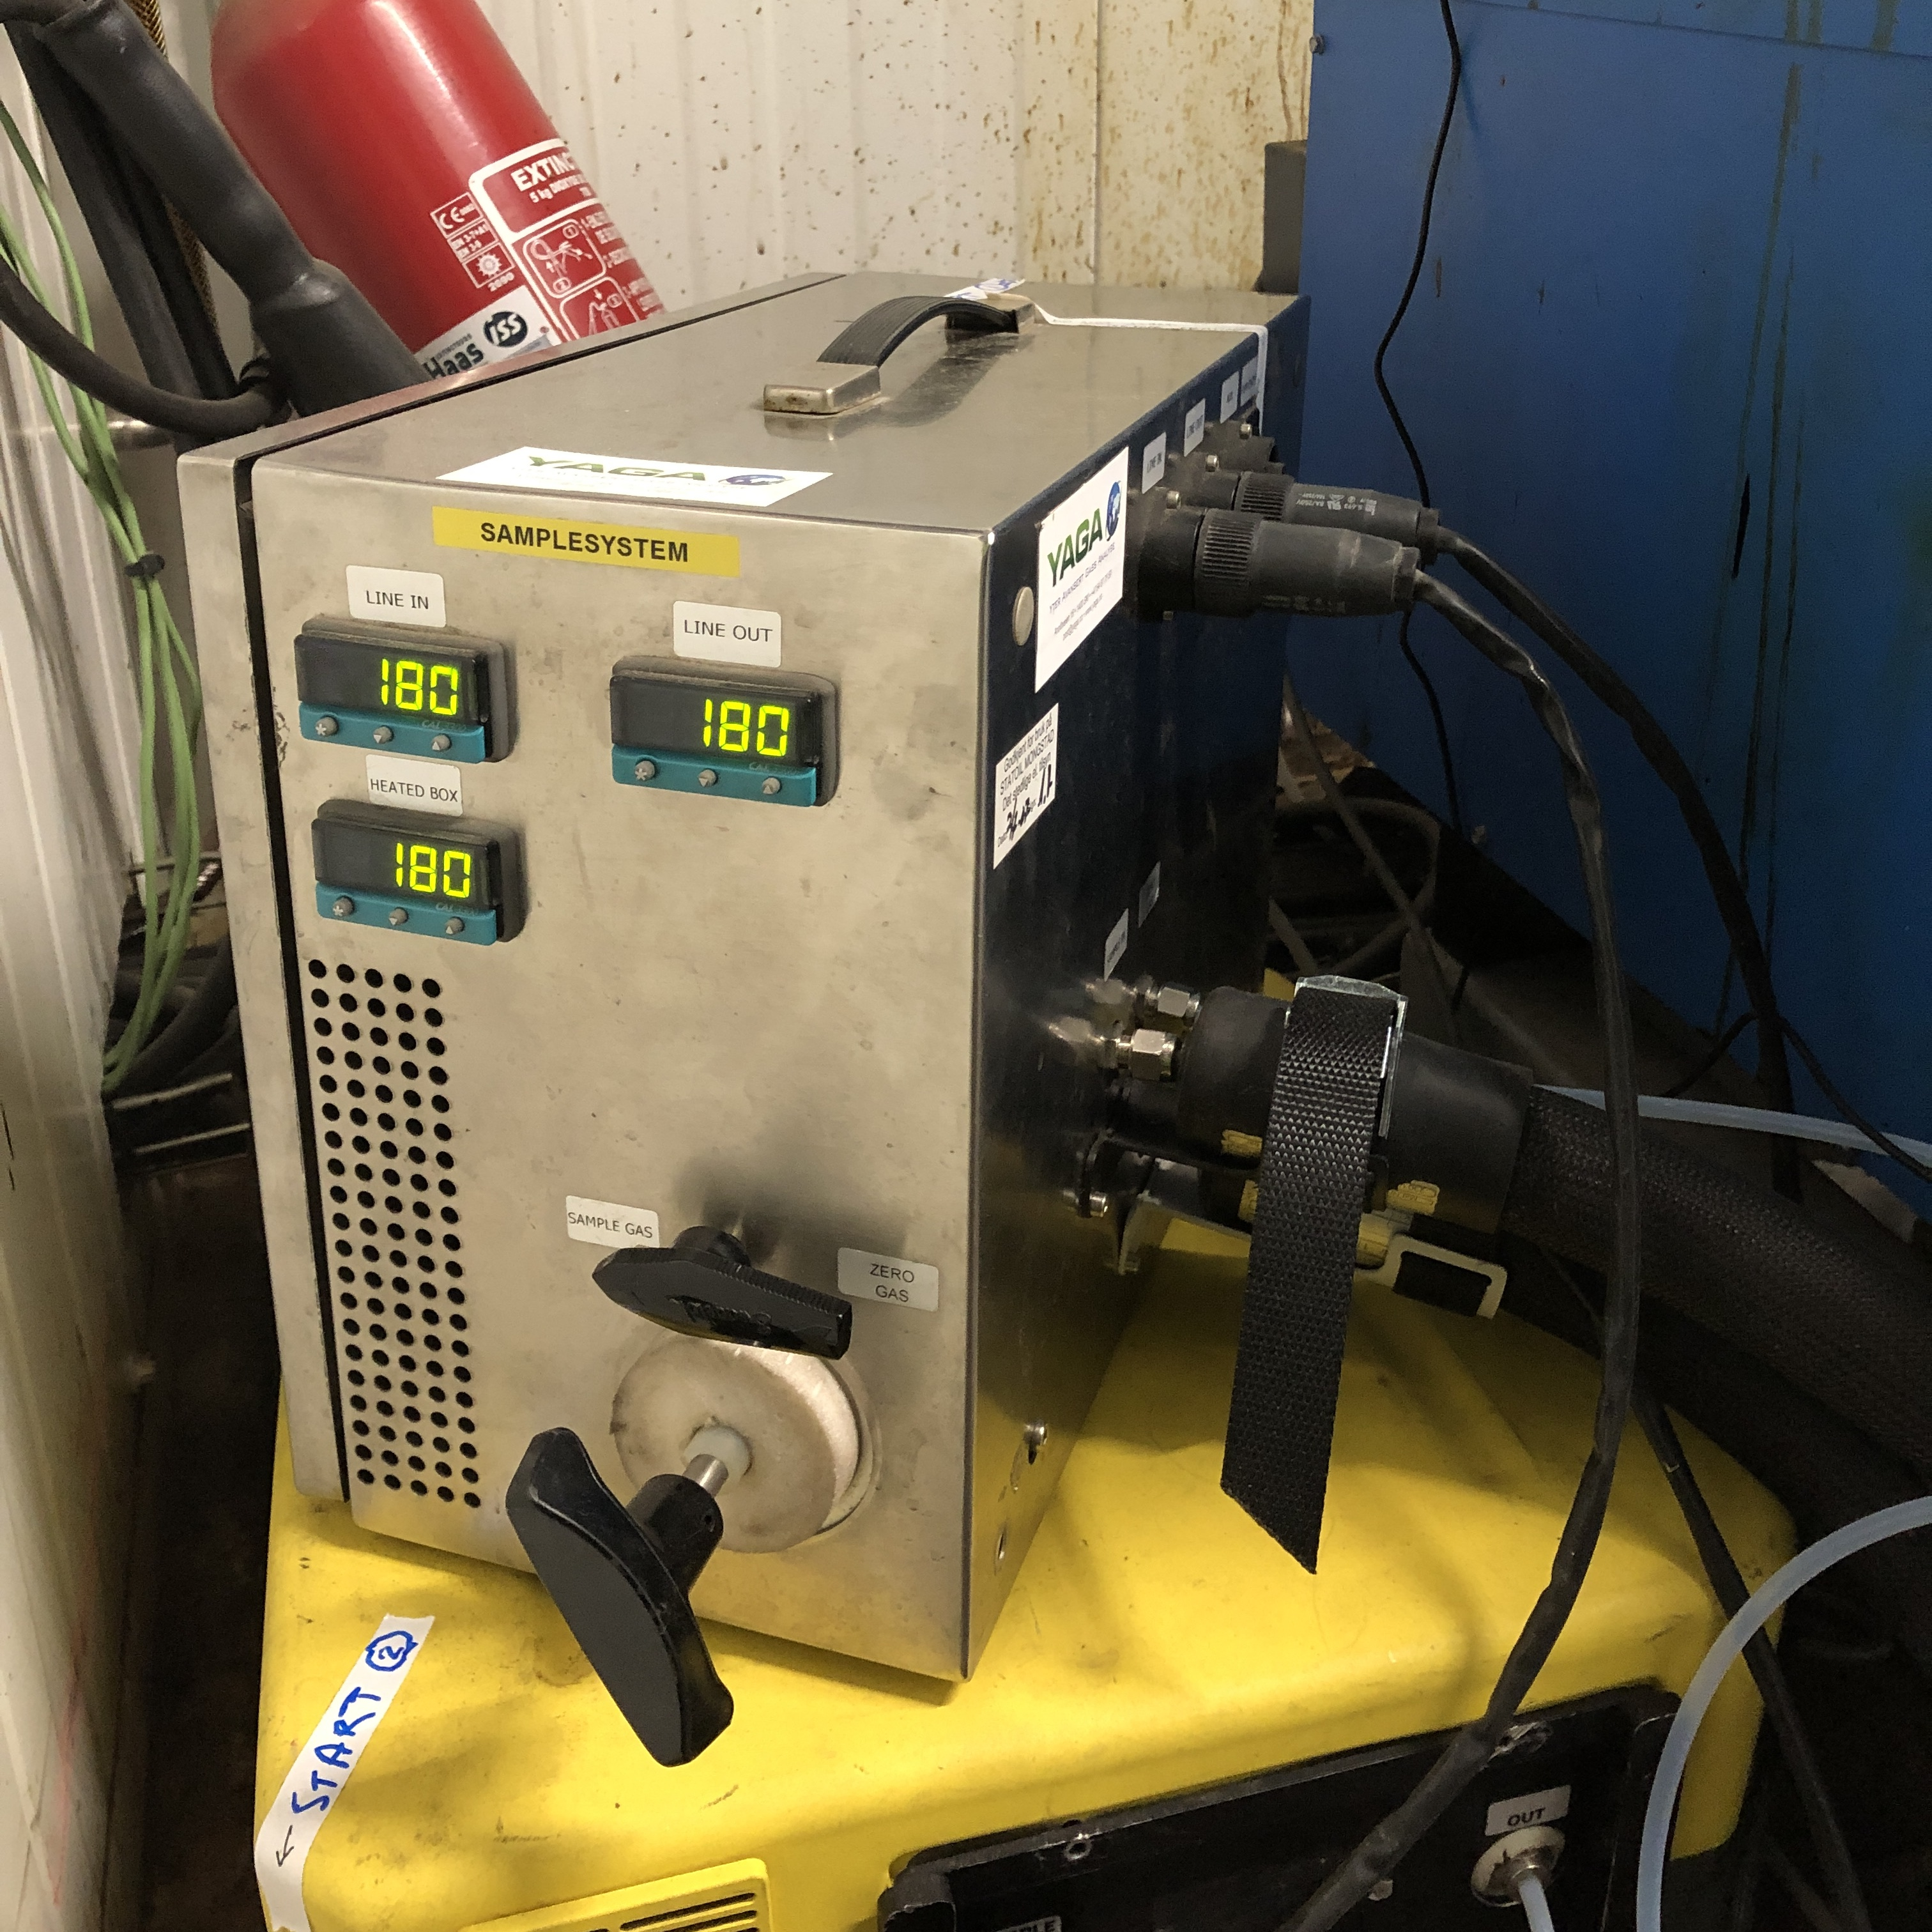
\includegraphics[width=0.6\textwidth]{Bilder/Pyrolysis/FTIR.jpg}
         \caption{}
         \label{appFig:FTIRbox}
     \end{subfigure}
     \hfill
     \begin{subfigure}[t]{\textwidth}
         \centering
         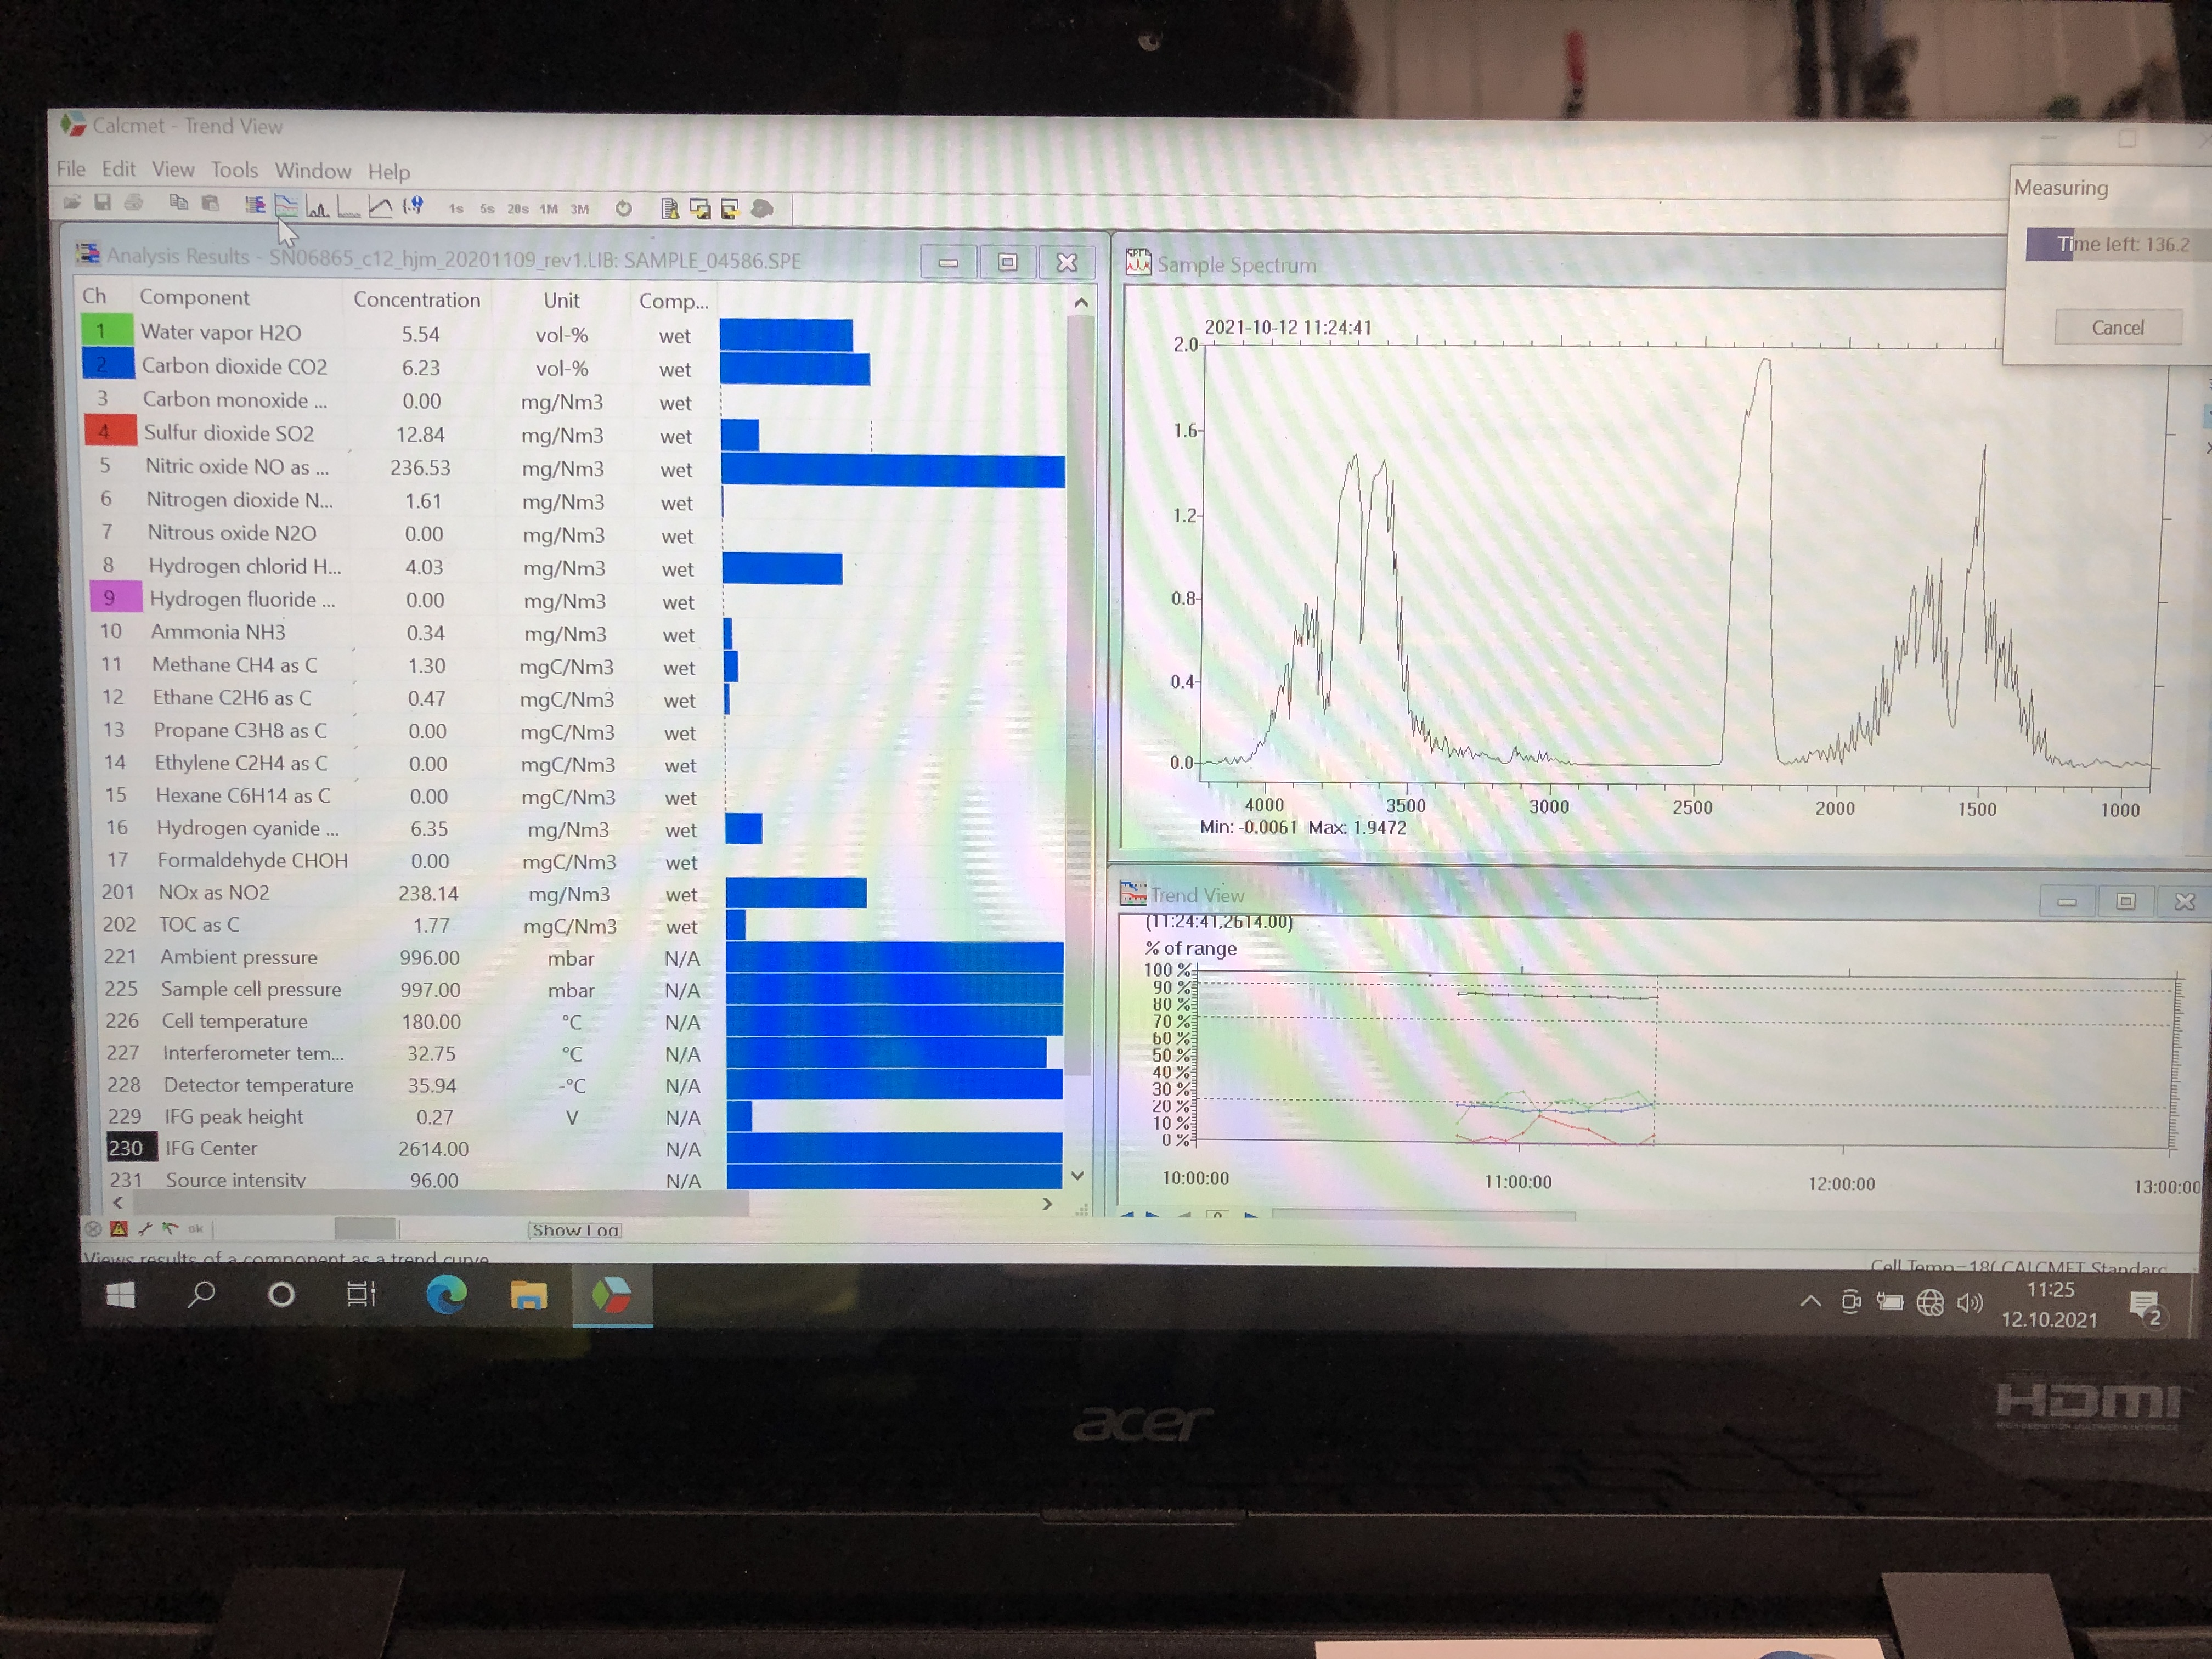
\includegraphics[width=0.6\textwidth]{Bilder/Pyrolysis/FTIRresults.png}
         \caption{}
         \label{appFig:FTIRresults}
     \end{subfigure}
     \hfill
     \caption{(a) FTIR. The tube leading to the FTIR is heated to 180 \textdegree C to prevent condensation of syn-gas. (b) FTIR output results. The results are a screenshot of the FTIR spectra from pyrolysis of Biorest Lindum (BRL).}
    \label{appFig:FTIR}
\end{figure}


\begin{figure}
    \centering
    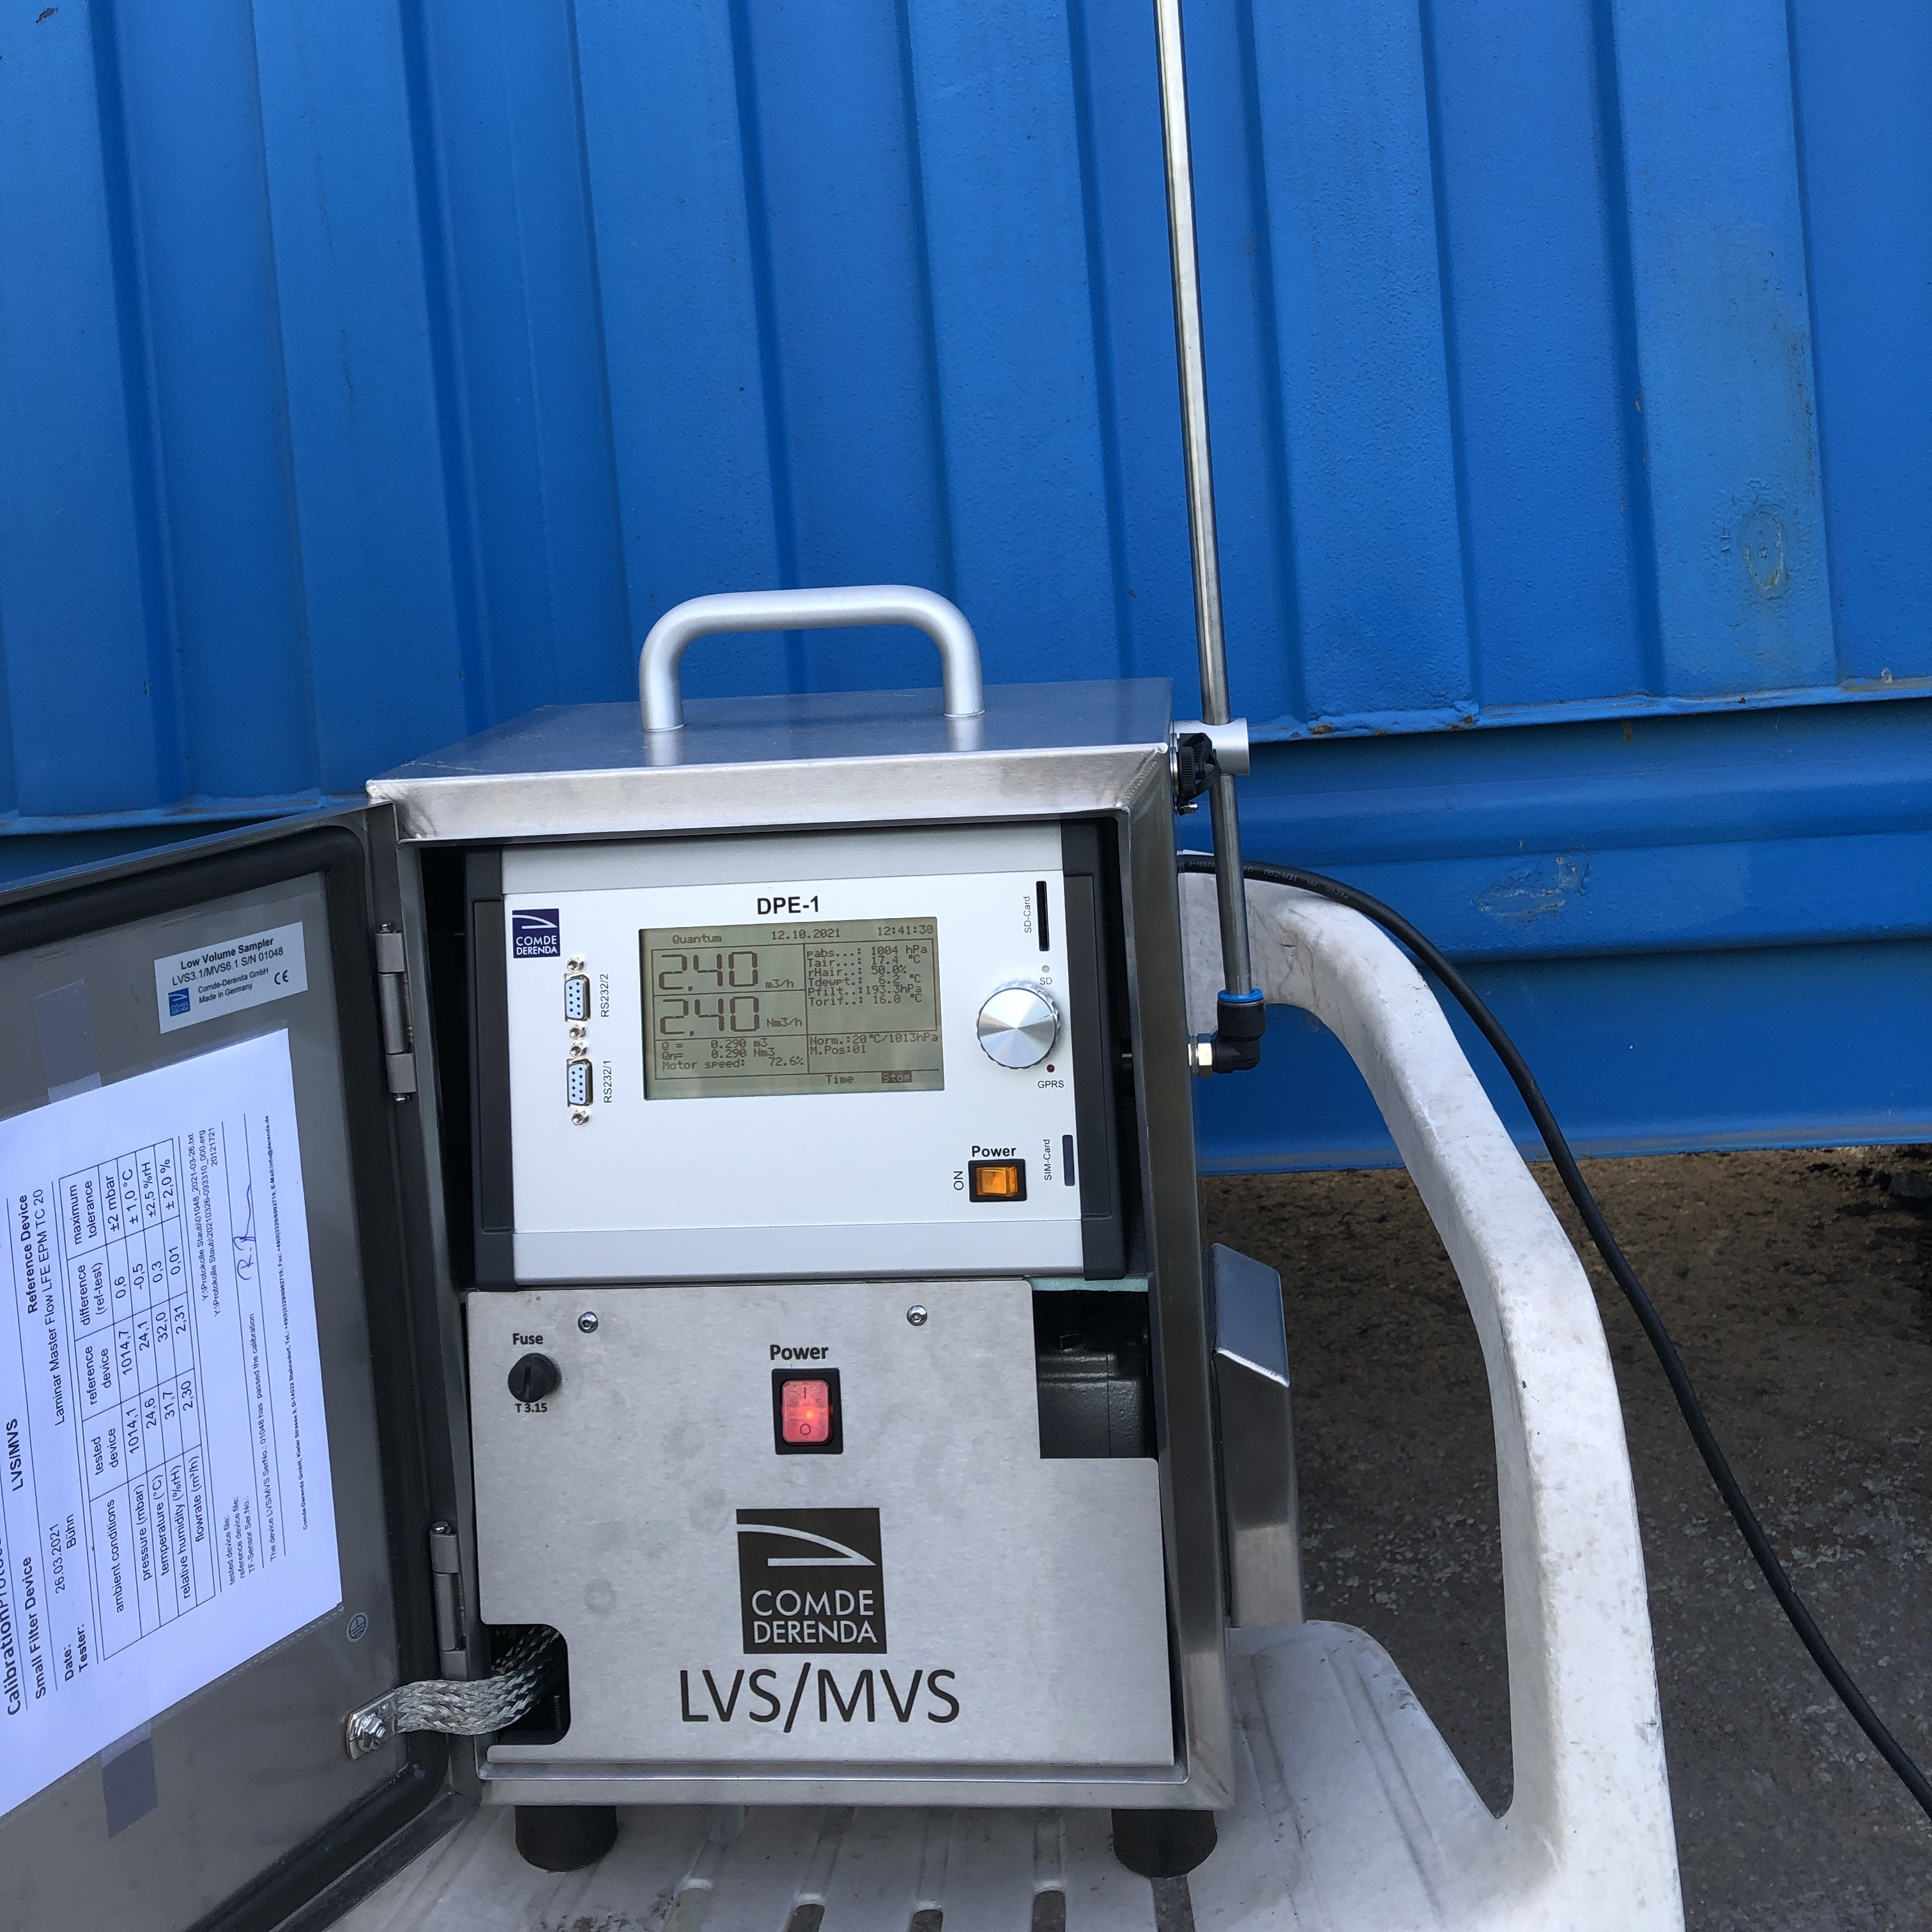
\includegraphics[width=0.85\textwidth]{Bilder/Pyrolysis/ParticlePump.jpg}
    \caption{LVS/MVS vacuum pump draws in air emitted from the ETIA chimney, and the sampler fractionates the airborne fine particles in a sampling inlet. The air containing the desired fine particulate fraction then passes through the filter, where the particles are collected and made available for subsequent gravimetric assessment or analysis. The volumetric flow rate is measured with an orifice plate and electronically adjusted with an accuracy of $\leq$ 2 $\%$. (Copied from comde-derenda.com, bust be rephrased)}
    \label{appFig:ParticlePump}
\end{figure}


\end{document}